%%%%%%%%------------------------------------------------------------------------
% This program is free software: you can redistribute it and/or modify
% it under the terms of the GNU General Public License as published by
% the Free Software Foundation, either version 3 of the License, or
% (at your option) any later version.
% 
% This program is distributed in the hope that it will be useful,
% but WITHOUT ANY WARRANTY; without even the implied warranty of
% MERCHANTABILITY or FITNESS FOR A PARTICULAR PURPOSE.  See the
% GNU General Public License for more details.
% 
% You should have received a copy of the GNU General Public License
% along with this program.  If not, see <http://www.gnu.org/licenses/>.

%%%%%%%%------------------------------------------------------------------------
%%%% 导言区 
%% 文档类型为article
\documentclass[a4paper, 10pt]{book}
%1m = 39.4 inch
%大18开 (18.5cm * 23cm)
%\usepackage[left=3.25cm, right=3.25cm, top=2.3cm,bottom=1.4cm]{geometry}
\usepackage{geometry}
\geometry{left=3.75cm,right=3.25cm,top=3cm,bottom=2.5cm}

%% en_preamble包含基本的宏包配置
%%%%%%%%------------------------------------------------------------------------
%%%% 日常所用宏包

%%设置行间距
\usepackage{setspace}

%% 控制项目列表
\usepackage{enumerate}

%% 多栏显示
\usepackage{multicol}

%% hyperref宏包,生成可定位点击的超链接,并且会生成pdf书签
\usepackage[%
    pdfstartview=FitH,%
    CJKbookmarks=true,%
    bookmarks=true,%
    bookmarksnumbered=true,%
    bookmarksopen=true,%
    colorlinks=true,%
    citecolor=blue,%
    linkcolor=blue,%
    anchorcolor=green,%
    urlcolor=blue%
]{hyperref}

%% 控制标题
\usepackage{titlesec}

%% 控制表格样式
\usepackage{booktabs}

%% 控制目录
\usepackage{titletoc}

%% 控制字体大小
\usepackage{type1cm}

%% 首行缩进,用\noindent取消某段缩进
\usepackage{indentfirst}

%% 支持彩色文本、底色、文本框等
\usepackage{color,xcolor}

%% AMS LaTeX宏包
\usepackage{amsmath}
\usepackage{amssymb}

%% 一些特殊符号
% \usepackage{bbding}

%% 支持引用
% \usepackage{cite}

%% LaTeX一些特殊符号宏包
% \usepackage{latexsym}

%% 数学公式中的黑斜体
% \usepackage{bm}

%% 调整公式字体大小:\mathsmaller, \mathlarger
% \usepackage{relsize}

%% 生成索引
% \makeindex

%%%% 基本插图方法
%% 图形宏包
\usepackage{graphicx}
\usepackage{float}
%% 如果插入的图片没有指定扩展名,那么依次搜索下面的扩展名所对应的文件
\DeclareGraphicsExtensions{.pdf,.eps,.png,.jpg}
%% 让 latex 从 .bb 中读取 Bounding Box 信息
%\DeclareGraphicsRule{.jpg}{eps}{.bb}{}
%\DeclareGraphicsRule{.png}{eps}{.bb}{}
%\DeclareGraphicsRule{.pdf}{eps}{.bb}{}

%% 多个图形并排,参加lnotes.pdf
%\usepackage{subfig}
\usepackage{subfigure}


\usepackage{caption}
\captionsetup{font={sf, scriptsize}, labelfont={bf}, skip=15pt}
\DeclareCaptionLabelSeparator{colon}{~~}

\usepackage[perpage,stable]{footmisc}

\usepackage{longtable}
% \begin{figure}[htbp]               %% 控制插图位置
%   \setlength{\abovecaptionskip}{0pt}
%   \setlength{\belowcaptionskip}{10pt}
                                     %% 控制图形和上下文的距离
%   \centering                       %% 使图形居中显示
%   \includegraphics[width=0.8\textwidth]{CTeXLive2008.jpg}
                                     %% 控制图形显示宽度为0.8\textwidth
%   \caption{CTeXLive2008安装过程} \label{fig:CTeXLive2008}
                                     %% 图形题目和交叉引用标签
% \end{figure}
%%%% 基本插图方法结束

%%%% pgf/tikz绘图宏包设置
\usepackage{pgf,tikz}
\usetikzlibrary{shapes,automata,snakes,backgrounds,arrows}
\usetikzlibrary{mindmap, trees,  calendar}
\usetikzlibrary{positioning}
\usepackage{pgf-umlsd}
%% 可以直接在latex文档中使用graphviz/dot语言,
%% 也可以用dot2tex工具将dot文件转换成tex文件再include进来
%% \usepackage[shell,pgf,outputdir={docgraphs/}]{dot2texi}
%%%% pgf/tikz设置结束


%%%% fancyhdr设置页眉页脚
%% 页眉页脚宏包
\usepackage{fancyhdr}

%% 页眉页脚风格
\pagestyle{fancy}

%%这两行代码是修改\leftmark和\rightmark的经典模式
\renewcommand{\chaptermark}[1]{\markboth{{\hei {第\thechapter{}章}}\hspace 1  #1}{}}
\renewcommand{\sectionmark}[1]{\markright{\thesection{} #1}}

%% 清空当前页眉页脚的默认设置
\fancyhf{}

%\fancyhead[L]{\scriptsize \fangsong \ascii{ZTE}中兴}
%\fancyhead[R]{\scriptsize \fangsong 内部公开}

%\fancyhead[CE]{\scriptsize \fangsong \leftmark}
%\fancyhead[CO]{\scriptsize \fangsong \rightmark}

%\fancyfoot[RO, LE]{\scriptsize \thepage}
%\fancyfoot[C]{\scriptsize \fangsong 本文中的所有信息均为中兴通讯股份有限公司内部信息,不得向外传播}

\renewcommand{\headrulewidth}{0.4pt}
\renewcommand{\footrulewidth}{0.4pt}

%第{\couriernew\thechapter{}}章
%%下面开始修改页眉和页脚
\fancyhead[RE]{\fangsong \leftmark}
\fancyhead[LO]{\fangsong \rightmark}
\fancyhead[RO, LE]{\small \thepage}
\fancypagestyle{plain}{%
  \fancyhead{} % get rid of headers
  \renewcommand{\headrulewidth}{0pt} % and the line.
}

%%定义空白页面
\makeatletter
\def\cleardoublepage{\clearpage\if@twoside \ifodd\c@page\else
  \hbox{}
  \vspace*{\fill}
  \begin{center}
   {\sffamily\large}
   \end{center}
   \vspace{\fill}
   \thispagestyle{empty}
   \newpage
   \if@twocolumn\hbox{}\newpage\fi\fi\fi}
\makeatother

\makeatletter
\def\cleardedicatepage{\clearpage
  \hbox{}
  \vspace*{\fill}
  \begin{center}
   {\sffamily\Large 献给我的女儿刘楚溪}
   \end{center}
   \vspace{\fill}
   \thispagestyle{empty}
   \newpage
   \if@twocolumn\hbox{}\newpage\fi}
\makeatother

%% 有时会出现\headheight too small的warning
\setlength{\headheight}{15pt}
%%%% fancyhdr设置结束

%%设置行间距离
\usepackage{framed}  
%%%% listings宏包设置结束

%%%% 附录设置
\usepackage[title,titletoc,header]{appendix}
%%%% 附录设置结束

%%%% 日常宏包设置结束
%%%%%%%%------------------------------------------------------------------------

%%%%%%%%------------------------------------------------------------------------
%%%% 英文字体设置结束
%% 这里可以加入自己的英文字体设置
%%%%%%%%------------------------------------------------------------------------

%%%%%%%%------------------------------------------------------------------------
%%%% 设置常用字体字号,与MS Word相对应

%% 一号, 1.4倍行距
\newcommand{\yihao}{\fontsize{26pt}{36pt}\selectfont}
%% 二号, 1.25倍行距
\newcommand{\erhao}{\fontsize{22pt}{28pt}\selectfont}
%% 小二, 单倍行距
\newcommand{\xiaoer}{\fontsize{18pt}{18pt}\selectfont}
%% 三号, 1.5倍行距
\newcommand{\sanhao}{\fontsize{16pt}{24pt}\selectfont}
%% 小三, 1.5倍行距
\newcommand{\xiaosan}{\fontsize{15pt}{22pt}\selectfont}
%% 四号, 1.5倍行距
\newcommand{\sihao}{\fontsize{14pt}{21pt}\selectfont}
%% 半四, 1.5倍行距
\newcommand{\bansi}{\fontsize{13pt}{19.5pt}\selectfont}
%% 小四, 1.5倍行距
\newcommand{\xiaosi}{\fontsize{12pt}{18pt}\selectfont}
%% 大五, 单倍行距
\newcommand{\dawu}{\fontsize{11pt}{11pt}\selectfont}
%% 五号, 单倍行距
\newcommand{\wuhao}{\fontsize{10.5pt}{10.5pt}\selectfont}
%%%%%%%%------------------------------------------------------------------------

%%%%%%%%------------------------------------------------------------------------
%%%% 一些个性设置

%% 设定页码方式,包括arabic、roman等方式
%% \pagenumbering{arabic}

%% 有时LaTeX无从断行,产生overfull的错误,这条命令降低LaTeX断行标准
%% \sloppy

%% 设定目录显示深度\tableofcontents
%% \setcounter{tocdepth}{2}
%% 设定\listoftables显示深度
%% \setcounter{lotdepth}{2}
%% 设定\listoffigures显示深度
%% \setcounter{lofdepth}{2}

%% 中文破折号,据说来自清华模板
\newcommand{\pozhehao}{\kern0.3ex\rule[0.8ex]{2em}{0.1ex}\kern0.3ex}

%% 设定itemize环境item的符号
\renewcommand{\labelitemi}{$\bullet$}

%\makeatletter
%\@addtoreset{lstlisting}{section} 
%\makeatother

\newenvironment{enum}
{
  \begin{spacing}{1.2}
  \begin{enumerate}[1.]
    \setlength{\itemsep}{0pt} 
    \setlength{\itemindent}{2em}
    %\setlength{\listparindent}{2em}
}{%
  \end{enumerate}
  \end{spacing}
}

\newcommand{\suggest}[1]{
\tikzstyle{mybox} = [draw=black, very thick,
rectangle, rounded corners, inner sep=9pt, inner ysep=20pt]
\tikzstyle{fancytitle} =[fill=white, text=black, ellipse]
\noindent
\begin{tikzpicture}
\node [mybox] (box){%
\begin{minipage}{\textwidth}
\fangsong
#1
\end{minipage}
};
\node[fancytitle, right=10pt] at (box.north west) {\emph{建议}};
% \node[fancytitle, rounded corners] at (box.east) {$\clubsuit$};
\end{tikzpicture}
}

\newcommand{\notice}[1]{
\tikzstyle{mybox} = [draw=black, very thick,
rectangle, rounded corners, inner sep=9pt, inner ysep=20pt]
\tikzstyle{fancytitle} =[fill=white, text=black]
\noindent
\begin{tikzpicture}
\node [mybox] (box){%
\begin{minipage}{\textwidth}
\fangsong
#1
\end{minipage}
};
\node[fancytitle, right=10pt] at (box.north west) {\emph{注意}};
%\node[fancytitle, rounded corners] at (box.east) {$\clubsuit$};
\end{tikzpicture}
}

\newcommand{\tip}[1]{
\tikzstyle{mybox} = [draw=black, very thick,
rectangle, rounded corners, inner sep=9pt, inner ysep=20pt]
\tikzstyle{fancytitle} =[fill=white, text=black]
\noindent
\begin{tikzpicture}
\node [mybox] (box){%
\begin{minipage}{\textwidth}
\fangsong
#1
\end{minipage}
};
\node[fancytitle, right=10pt] at (box.north west) {\emph{提示}};
%\node[fancytitle, rounded corners] at (box.east) {$\clubsuit$};
\end{tikzpicture}
}

\newcommand\refch[1]{\ascii{第\ref{ch:#1}章(\nameref{ch:#1})}}
\newcommand\refsec[1]{\ascii{\ref{sec:#1}节(\nameref{sec:#1})}}

\newcommand\eitem[1]{\item {\itshape {#1}}}
\newcommand\cpp{\ascii{C\nobreak+\nobreak+}}
\newcommand\clang{\ascii{C}}
\newcommand\tf{\ascii{TensorFlow}}

\newcommand\quo[1]{“#1”}

\newcommand\percent[1]{\ascii{#1\%}}

\newcommand{\trans}{\emph{事务}}
\newcommand{\act}{\emph{操作}}
\newcommand{\seqact}{\emph{顺序操作}}
\newcommand{\conact}{\emph{并发操作}}
\newcommand{\atomact}{\emph{基本操作}}
\newcommand{\syncact}{\emph{同步操作}}
\newcommand{\asynact}{\emph{异步操作}}
\newcommand{\action}[1]{\emph{\ascii{\itshape\_\_#1}}}
\newcommand{\sigwait}{\action{sig\_wait}}
\newcommand{\sigsync}{\action{sig\_sync}}
\newcommand{\sigreply}{\action{sig\_reply}}
\newcommand{\timerprot}{\action{timer\_prot}}
\newcommand{\unknownevet}{\ascii{UNKNOWN\_EVENT}}
\newcommand{\transdsl}{\ascii{Transaction DSL}}
\newcommand{\oper}[1]{\ascii{Action#1}}
\newcommand{\protproc}{\ascii{prot\_procedure}}

%\newcommand{\code}[1]{\ascii{\small{\texttt{#1}}}}
\newcommand{\code}[1]{\ascii{\footnotesize{\texttt{#1}}}}

%\newcommand{\Email}{\begingroup \def\UrlLeft{<}\def\UrlRight{>} \urlstyle{tt}\Url}
%\def\mailto|#1|{\href{mailto:#1}{Email|#1|}}
\newcommand{\contrib}[2]{#1\quad{\small\quad\textit{#2}}\\[1ex]}
%% 设定正文字体大小
% \renewcommand{\normalsize}{\sihao}

%%%% 个性设置结束
%%%%%%%%------------------------------------------------------------------------


%%%%%%%%------------------------------------------------------------------------
%%%% bibtex设置

%% 设定参考文献显示风格

%%%% bibtex设置结束
%%%%%%%%------------------------------------------------------------------------


%% 如果不写中文的话就不需要引用xecjk_preamble里面的配置
%%%%%%%%------------------------------------------------------------------------
%%%% xeCJK相关宏包

\usepackage{xltxtra,fontspec,xunicode}

%% \CJKsetecglue{\hskip 0.15em plus 0.05em minus 0.05em}
%% slanfont: 允许斜体
%% boldfont: 允许粗体
%% CJKnormalspaces: 仅忽略汉字之间的空白,但保留中英文之间的空白。 
%% CJKchecksingle: 避免单个汉字单独占一行。
\usepackage[slantfont, boldfont]{xeCJK} 

%% 针对中文进行断行
\XeTeXlinebreaklocale "zh"             

%% 给予TeX断行一定自由度
\XeTeXlinebreakskip = 0pt plus 1pt minus 0.1pt

%%%% xeCJK设置结束                                       
%%%%%%%%------------------------------------------------------------------------

%%%%%%%%------------------------------------------------------------------------
%%%% xeCJK字体设置

%% 设置中文标点样式,支持quanjiao、banjiao、kaiming等多种方式
\punctstyle{quanjiao}                                        
                                                     
%% 设置缺省中文字体
\setCJKmainfont[BoldFont={Adobe Heiti Std}, ItalicFont={Adobe Kaiti Std}]{Adobe Song Std}   %  FZBaoSongZ04
%% 设置中文无衬线字体
\setCJKsansfont[BoldFont={Adobe Heiti Std}, ItalicFont={Adobe Kaiti Std}]{Adobe Kaiti Std}  
%% 设置等宽字体
\setCJKmonofont{Adobe Heiti Std}                            
%\setCJKmonofont{Monaco}                            

%% 英文衬线字体
\setmainfont{Lucida Bright}                                  
%% 英文等宽字体
%\setmonofont{Courier}
\setmonofont{Monaco}                             
%\setmonofont{Consolas}                              
%% 英文无衬线字体
\setsansfont{Optima}                                   

%% 定义新字体
\setCJKfamilyfont{song}{Adobe Song Std}                     
\setCJKfamilyfont{kai}{Adobe Kaiti Std}
\setCJKfamilyfont{hei}{Adobe Heiti Std}
\setCJKfamilyfont{fangsong}{Adobe Song Std}
\setCJKfamilyfont{lisu}{LiShu}
\setCJKfamilyfont{youyuan}{Adobe Kaiti Std}

%%自定义英文字体
\newfontfamily\couriernew{Lucida Grande}
\newfontfamily\optima{Optima}
\newfontfamily\lucida{Lucida Bright}

\newcommand{\ascii}[1]{{\sffamily #1}}
\newcommand{\speak}[1]{{\itshape #1}}
\renewcommand{\emph}[1]{{\hei #1}}

%% 自定义宋体
\newcommand{\song}{\CJKfamily{song}}                       
%% 自定义楷体
\newcommand{\kai}{\CJKfamily{kai}}                         
%% 自定义黑体
\newcommand{\hei}{\CJKfamily{hei}}                         
%% 自定义仿宋体
\newcommand{\fangsong}{\CJKfamily{fangsong}}               
%% 自定义隶书
\newcommand{\lisu}{\CJKfamily{lisu}}                       
%% 自定义幼圆
\newcommand{\youyuan}{\CJKfamily{youyuan}}                 

%%%% xeCJK字体设置结束
%%%%%%%%------------------------------------------------------------------------

%%%%%%%%------------------------------------------------------------------------
%%%% 一些关于中文文档的重定义

%% 数学公式定理的重定义

\newtheorem{example}{例}[section]                                   
\newtheorem{algorithm}{算法}
%% 按section编号
\newtheorem{theorem}{定理}[section]                         
\newtheorem{definition}{定义}
\newtheorem{axiom}{公理}
\newtheorem{property}{性质}
\newtheorem{proposition}{命题}
\newtheorem{lemma}{引理}
\newtheorem{corollary}{推论}
\newtheorem{condition}{条件}
\newtheorem{conclusion}{结论}
\newtheorem{assumption}{假设}

\newtheorem{principle}{原则}[section]
\newtheorem{regulation}{规则}[section]
\newtheorem{advise}{建议}[section]
\newtheorem{concept}{概念}[section]

%% 章节等名称重定义
\renewcommand{\contentsname}{目录}     
%\renewcommand{\abstractname}{摘要}
\renewcommand{\indexname}{索引}
\renewcommand{\listfigurename}{插图目录}
\renewcommand{\listtablename}{表格目录}
\renewcommand{\figurename}{图}
\renewcommand{\tablename}{表}
\renewcommand{\appendixname}{附录}
\renewcommand{\appendixpagename}{附录}
\renewcommand{\appendixtocname}{附录}
%\renewcommand\refname{参考文献} 

%%设置内容环境
\newenvironment{content}{%
  \setlength{\parskip}{0.5\baselineskip}
  \begin{spacing}{1.5}
}{%
  \end{spacing}
  \setlength{\parskip}{-0.5\baselineskip}
  \vskip -0.5\baselineskip
}

% 插入小段故事的语法:
% \begin{story}
%   \begin{center}
%     \inlinetitle{分水岭}
%   \end{center}
% \end{story}
\newenvironment{story}
{
  \setlength{\parskip}{0.5\baselineskip}
  \hbox to \textwidth{\hfil\rule{\linewidth}{0.5mm}\hfil}
  \begin{spacing}{1.5}
}{%
  \end{spacing}
  \hbox to \textwidth{\hfil\rule{\linewidth}{0.5mm}\hfil}
  \setlength{\parskip}{-0.5\baselineskip}
  \vskip -0.5\baselineskip
}

%% 设置chapter、section与subsection的格式
%\titleformat{\chapter}[display]{\flushright\yihao}{\thechapter{}}{1em}{\textbf}
\titleformat{\section}[block]{\flushleft\sanhao}{\optima{\thesection}}{1em}{\textbf}
\titleformat{\subsection}{\sihao}{\optima{\thesubsection}}{0.5em}{\textbf}
\titleformat{\subsubsection}{\xiaosi}{\thesubsubsection}{0.5em}{\textbf}

%\titlespacing{\chapter}{0pt}{0pt}{-\baselineskip}
\titlespacing{\section}{0pt}{0pt}{0\baselineskip}
\titlespacing{\subsection}{0pt}{0.5\baselineskip}{0\baselineskip}

%% 设置章格式
\usepackage{quotchap}

\renewcommand\chapterheadstartvskip{
   \vspace*{-5\baselineskip}
}

\renewcommand\chapterheadendvskip{
   \vspace*{0.5\baselineskip}
}

\usepackage{helvet}
\renewcommand\sectfont{\rmfamily\bfseries}

\newcommand\refig[1]{{\itshape \figurename\ascii{\ref{fig:#1}(第\pageref{fig:#1}页)}}}
\newcommand\reftbl[1]{{\itshape \tablename\ascii{\ref{tbl:#1}(第\pageref{tbl:#1}页)}}}

\renewcommand{\footnoterule}{\vspace*{3pt}%
  \hrule width 0.382\textwidth height 0.4pt \vspace*{2.6pt}}

% Remark
\newenvironment{remark}{\par\vskip10pt\footnotesize\itshape % Vertical white space above the remark and smaller font size
\begin{list}{}{
\leftmargin=35pt % Indentation on the left
\rightmargin=25pt}\item\ignorespaces % Indentation on the right
\makebox[-2.5pt]{\begin{tikzpicture}[overlay]
\node[draw=red!60,line width=1pt,circle,fill=red!25,font=\sffamily\bfseries,inner sep=2pt,outer sep=0pt] at (-15pt,0pt){\textcolor{red}{R}};\end{tikzpicture}}
\advance\baselineskip -1pt}{\end{list}\vskip5pt}

%%%% 中文重定义结束
%%%%%%%%------------------------------------------------------------------------


%%%% 设置listings宏包用来粘贴源代码
%% 方便粘贴源代码,部分代码高亮功能
\usepackage{listings}
\usepackage{color}

\DeclareCaptionFont{red}{\color{red}}

%% 所要粘贴代码的编程语言
\lstloadlanguages{{[LaTeX]TeX}, {[ISO]C++}, {Java}, {Ruby}, {Python}, {Scala}}

%% 设置listings宏包的一些全局样式
%% 参考http://hi.baidu.com/shawpinlee/blog/item/9ec431cbae28e41cbe09e6e4.html
\lstset{
numberbychapter=true,
breakatwhitespace=true,
showstringspaces=false,              %% 设定是否显示代码之间的空格符号
basicstyle=\footnotesize\ttfamily,           %% 设定字体大小\tiny, \scriptsize, \footnotesize, \small, \Large等等
keywordstyle=\bfseries,
commentstyle=\color{red!50!green!50!blue!50},                           
escapechar=`,                        %% 中文逃逸字符,用于中英混排
xleftmargin=1.5em,xrightmargin=0em, aboveskip=1em,
breaklines,                          %% 这条命令可以让LaTeX自动将长的代码行换行排版
extendedchars=false,                 %% 这一条命令可以解决代码跨页时,章节标题,页眉等汉字不显示的问题
frameround=fttt,
captionpos=top,
belowcaptionskip=1em
}

\lstdefinestyle{numbers}{
   numbers=left,
   numberstyle=\tiny,
   stepnumber=1,
   numbersep=1em
}

\lstdefinestyle{C++}{
   language=C++,
   texcl=true,
   prebreak=\textbackslash,
   breakindent=1em,
   keywordstyle=\bfseries, %% 关键字高亮
   morekeywords={alignas, alignof, char16_t, char32_t, constexpr, decltype, noexcept, nullptr, static_assert, thread_local, override, OVERRIDE, INTERFACE, ABSTRACT, DEFINE_ROLE, ROLE, HAS_ROLE, USE_ROLE}
   style=numbers,
   %frame=leftline,                     %% 给代码加框
   %framerule=2pt,
   %rulesep=5pt
}

\lstnewenvironment{c++}[1][]
  {\setstretch{1}
  \lstset{style=C++, #1}}
  {}

%\captionsetup[lstlisting]{textfont=red}
%{labelfont=bf, singlelinecheck=off, labelsep=space, textfont=red}

\lstdefinestyle{Java}{
   language=Java,
   texcl=true,
   prebreak=\textbackslash,
   breakindent=1em,
   keywordstyle=\bfseries, %% 关键字高亮
   morekeywords={}
   style=numbers,
   %frame=leftline,                     %% 给代码加框
   %framerule=2pt,
   %rulesep=5pt
}

\lstnewenvironment{java}[1][]
  {\setstretch{1}
  \lstset{style=Java, #1}}
  {}

\lstdefinestyle{Ruby}{
   language=Java,
   texcl=true,
   prebreak=\textbackslash,
   breakindent=1em,
   keywordstyle=\bfseries, %% 关键字高亮
   morekeywords={}
   style=numbers,
   %frame=leftline,                     %% 给代码加框
   %framerule=2pt,
   %rulesep=5pt
}

\lstnewenvironment{ruby}[1][]
  {\setstretch{1}
  \lstset{style=Ruby, #1}}
  {}

\lstdefinestyle{Python}{
   language=Python,
   texcl=true,
   prebreak=\textbackslash,
   breakindent=1em,
   keywordstyle=\bfseries, %% 关键字高亮
   morekeywords={}
   style=numbers,
   %frame=leftline,                     %% 给代码加框
   %framerule=2pt,
   %rulesep=5pt
}

\lstnewenvironment{python}[1][]
  {\setstretch{1}
  \lstset{style=Python, #1}}
  {}

\lstdefinestyle{Scala}{
   language=Scala,
   texcl=true,
   prebreak=\textbackslash,
   breakindent=1em,
   keywordstyle=\bfseries, %% 关键字高亮
   morekeywords={}
   style=numbers,
   %frame=leftline,                     %% 给代码加框
   %framerule=2pt,
   %rulesep=5pt
}

\lstnewenvironment{scala}[1][]
  {\setstretch{1}
  \lstset{style=Scala, #1}}
  {}  

\renewcommand{\lstlistingname}{示例代码}
\renewcommand\thefigure{\thechapter-\arabic{figure}}

\newcommand\refcode[1]{{\itshape \lstlistingname\ascii{\ref{code:#1}(第\pageref{code:#1}页)}}}


% \usepackage[
%   placement=center,
%   angle=45,
%   scale=4,
%   color=black!40,
%   %hshift=60,
%   %vshift=-5
% ]{background}

% \backgroundsetup{contents={TensorFlow Internals}}
%\backgroundsetup{contents={\includegraphics[width=0.2\textwidth]{figures/cock.jpg}}}

\newcommand{\myclearpage}{\clearpage{\pagestyle{empty}\cleardoublepage}}
\newcommand{\mydedicate}{\clearpage{\pagestyle{empty}\cleardedicatepage}}

%%%% 导言区结束
%%%%%%%%------------------------------------------------------------------------

%%%%%%%%------------------------------------------------------------------------
%%%% 正文部分

\begin{document}

\frontmatter
\pagestyle{empty}

%%自定义封面
\def\titlename{TensorFlow内核剖析}
\def\subtitle{TensorFlow Internals}
\def\authors{刘光聪\ 著}
% \def\orgnization{\ascii{ZTE \textcopyright 2014}}

% 
\newlength{\centeroffset}
\setlength{\centeroffset}{-0.5\oddsidemargin}
\addtolength{\centeroffset}{0.5\evensidemargin}
\thispagestyle{empty}

% \begin{tikzpicture}
%   \path[mindmap,concept color=black,text=white]
%     node[concept] {\ascii{Programming}}
%     [clockwise from=0]
%     child[concept color=green!50!black] {
%       node[concept] {\ascii{XP}}
%       [clockwise from=90]
%       child { node[concept] {\ascii{Simple Design}} }
%       child { node[concept] {\ascii{TDD}} }
%       child { node[concept] {\ascii{Refactoring}} }
%       child { node[concept] {\ascii{Pair Programming}} }
%     }
%     child[concept color=blue] {
%       node[concept] {\ascii{Oriented-Object}}
%       [clockwise from=-30]
%       child { node[concept] {\ascii{C++}} }
%       child { node[concept] {\ascii{Java}} }
%     }
%     child[concept color=red]
%     { node[concept] {\ascii{Evolutionary Design}} }
%     child[concept color=orange]
%     { node[concept] {\ascii{Clean Code}} };
%  \end{tikzpicture}

%title and subtitle
\vspace*{\stretch{1}}
\noindent\hspace*{\centeroffset}\makebox[0pt][l]{\begin{minipage}{\textwidth}
\flushright
{\Huge \hei \bfseries \titlename}
\noindent\rule[-1ex]{\textwidth}{5pt}\\[2.5ex]
\hfill\emph{\subtitle}
\end{minipage}}

%author
\vspace{\stretch{2}}
\noindent\hspace*{\centeroffset}\makebox[0pt][l]{\begin{minipage}{\textwidth}
\center
{\bfseries \authors} \\[1.5ex]
{\bfseries \orgnization}
\end{minipage}}

\vspace{\stretch{1}}

\pagebreak

% \myclearpage

% \mydedicate

% \input{contents/foreword}
% \myclearpage

% \chapter{前言} 
\label{ch:preface}

\section*{本书定位}

\begin{content}

这是一本剖析\ascii{TensorFlow}内核工作原理的书籍,并非讲述如何使用\ascii{TensorFlow}构建机器学习模型,也不会讲述应用\ascii{TensorFlow}的最佳实践。本书将通过剖析\ascii{TensorFlow}源代码的方式,揭示\ascii{TensorFlow}的系统架构、领域模型、工作原理、及其实现模式等相关内容,以便揭示内在的知识。

\end{content}


\section*{面向的读者}

\begin{content}

本书假设读者已经了解机器学习相关基本概念与理论,了解机器学习相关的基本方法论;同时,假设读者熟悉\ascii{Python, C++}等程序设计语言。

本书适合于渴望深入了解\ascii{TensorFlow}内核设计,期望改善\ascii{TensorFlow}系统设计和性能优化,及其探究\ascii{TensorFlow}关键技术的设计和实现的系统架构师、\ascii{AI}算法工程师、和\ascii{AI}软件工程师。

\end{content}

\section*{阅读方式}

\begin{content}

初次阅读本书,推荐循序渐进的阅读方式;对于高级用户,可以选择感兴趣的章节阅读。首次使用\ascii{TensorFlow}时,推荐从源代码完整地构建一次\ascii{TensorFlow},以便了解系统的构建方式,及其理顺所依赖的基本组件库。

另外,推荐使用\ascii{TensorFlow}亲自实践一些具体应用,以便加深对\ascii{TensorFlow}系统行为的认识和理解,熟悉常见\ascii{API}的使用方法和工作原理。强烈推荐阅读本书的同时,阅读\ascii{TensorFlow}关键代码;关于阅读代码的最佳实践,请查阅本书附录\ascii{A}的内容。

\end{content}

\section*{版本说明}

\begin{content}

本书写作时,\ascii{TensorFlow}稳定发布版本为\ascii{1.2}。不排除本书讲解的部分\ascii{API}将来被废弃,也不保证某些系统实现在未来版本发生变化,甚至被删除。

同时,为了更直接的阐述问题的本质,书中部分代码做了局部的重构;删除了部分异常处理分支,或日志打印,甚至是某些可选参数列表。但是,这样的局部重构,不会影响读者理解系统的主要行为特征,更有利于读者掌握系统的工作原理。

同时,为了简化计算图的表达,本书中的计算图并非来自\ascii{TensorBoard},而是采用简化了的,等价的图结构。同样地,简化了的图结构,也不会降低读者对真实图结构的认识和理解。

\end{content}

\section*{英语术语}

\begin{content}

因为我所撰写的文章,是供相关专业人士阅读,而非科普读物,因此在书中保留专业领域中朗朗上口的英语术语,故意不做翻译。例如,书中直接使用\ascii{OP}的术语,而不是将其翻译为「操作」。

但是,这会造成大面积的中英混杂的表达方式。幸运的是,绝对部分所使用的英语术语都是名词,极少出现动词或者形容词。但是,无论如何都不会丢失原本的主体语义和逻辑。

万事都有例外,对于无歧义的,表达简短,且语义明确的术语,会使用中文术语表示。特殊地,对于中文术语表达存在歧义时,会同时标注中文术语和英语术语。例如,检查点(\ascii{Checkpoint}),协调器(\ascii{Coordinator})。

一般地,无歧义的中文术语表定义在\reftbl{glossary}。

\begin{table}[!htb]
\resizebox{0.95\textwidth}{!} {
\begin{tabular*}{1.2\textwidth}{@{}ll@{}}
\toprule
\ascii{英文} & \ascii{中文} \\
\midrule
\ascii{Variable} & \ascii{变量,参数} \\
\ascii{Session} & \ascii{会话} \\ 
\ascii{Device} & \ascii{设备} \\ 
\bottomrule
\end{tabular*}
}
\caption{规范约定}
\label{tbl:glossary}
\end{table}

\end{content}

\section*{在线帮助}

\begin{content}

为了更好地与读者交流,在我的\ascii{Github}上建立了勘误表,及其相关补充说明。由于个人经验与能力有限,在有限的时间内难免犯错。如果读者在阅读过程中,如果发现相关错误,请帮忙提交\ascii{Pull Request},避免他人掉入相同的陷阱之中,让知识分享变得更加通畅,更加轻松,我将不甚感激。

同时,欢迎关注我的简书。我将持续更新相关的文章,与更多的朋友一起学习和进步。

\begin{enum}
  \eitem{\ascii{Github: \script{\url{https://github.com/horance-liu/tensorflow-internals-errors}}}}
  \eitem{\ascii{简书:\script{\url{http://www.jianshu.com/u/49d1f3b7049e}}}}
\end{enum}

\end{content}

\section*{致谢}

\begin{content}

感谢我的太太刘梅红,在工作之余完成对本书的审校,并提出了诸多修改的一件。

\end{content}

% \myclearpage

% \tableofcontents
% \myclearpage

\def\thelstlisting{\thechapter-\arabic{lstlisting}}
%% 中文习惯是设定首行缩进为2em。
%% 注意此设置一定要在document环境之中,这可能与\setlength作用范围相关
\setlength{\parindent}{2em}

%%%%%%%%%%%%%%%%%%%%%%
%%开始正文,页面计数从正文开始
\mainmatter
\setcounter{page}{1}
\pagestyle{fancy}

% \part{基础知识}
% \begin{savequote}[45mm]
\ascii{Any fool can write code that a computer can understand. Good programmers write code that humans can understand.}
\qauthor{\ascii{- Martin Flower}}
\end{savequote}

\chapter{介绍} 
\label{ch:introduction}

\begin{content}

\ascii{TensorFlow}是一个支持大规模和异构环境的机器学习系统。它使用数据流图\ascii{(Dataflow Graph)}表示计算过程和共享状态,使用节点表示抽象计算,使用边表示数据流。

数据流图的节点被映射在集群中的多个机器,在一个机器内被映射在多个计算设备\ascii{(Device)}上,包括\ascii{CPU, GPU, TPU}。\ascii{TensorFlow}灵活的架构支持多种计算平台,包括台式机,服务器,移动终端等。

\tf{}最初由\ascii{Google Brain}的研究员和工程师们开发出来,用于开展机器学习和深度神经网络方面的研究,但\tf{}优异的通用性使其也可广泛用于其他领域的数值计算。

\end{content}

\section{前世今生}

\begin{content}

\tf{}是\ascii{DistBelief}的后继者,它站在巨人的肩膀上,革命性地重新设计架构设计,使得\tf{}在机器学习领域一鸣惊人,在社区中产生了重大的影响。

为了更好地理解\tf{}系统架构的优越性,得先从\ascii{DistBelief}谈起。

\end{content}

\subsection{前世:DistBelief}

\begin{content}

\ascii{DistBelief}是一个用于训练大规模神经网络的的分布式系统,是\ascii{Google}第一代分布式机器学习框架。自\ascii{2011}年以来,在\ascii{Google}内部大量使用\ascii{DistBelief}训练大规模的神经网络。

\end{content}

\subsubsection{编程模型}

\begin{content}

\ascii{DistBelief}的编程模型是基于层\ascii{(Layer)}的\ascii{DAG(Directed Acyclic Graph)}图。层可以看做是一种组合多个运算操作符的复合运算符,它完成特定的计算任务。

例如,全连接层完成$f({W^T}x + b)$的复合计算,包括输入与权重的矩阵乘法,随后再与偏置相加,最后在线性加权值的基础上实施非线性变换。

\end{content}

\subsubsection{架构}

\begin{content}

\ascii{DistBelief}使用参数服务器\ascii{(Parameter Server)}的系统架构,训练作业包括两个分离的进程:无状态的\ascii{Worker}进程,用于模型训练的计算;有状态的\ascii{PS(Parameter Server)}进程,用于维护模型参数。

如\refig{parameter-server}所示,在分布式训练过程中,各个模型备份\ascii{(Model Relica)}异步地从\ascii{PS}上拉取\ascii{(Fetch)}训练参数$w$,当完成一步迭代运算后,推送\ascii{(Push)}参数的梯度$ \nabla w $到\ascii{PS}上去,并完成参数更新。

\begin{figure}[!htbp]
\centering
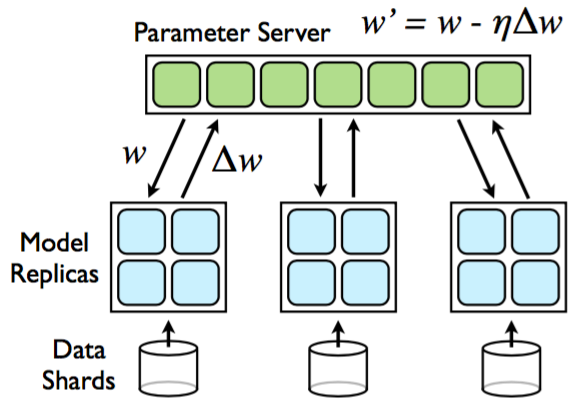
\includegraphics[width=0.6\textwidth]{figures/parameter-server.png}
\caption{DistBelief: Parameter Server架构}
 \label{fig:parameter-server}
\end{figure}

\end{content}

\subsubsection{缺陷与不足}

\begin{content}


但是,对于高级用户,\ascii{DistBelief}的编程模型,及其\ascii{Parameter Server}的系统架构,缺乏如下几个方面的扩展性。

\begin{enum}
  \eitem{优化算法:添加新的优化算法,必须修改\ascii{Parameter Server}的实现;\code{get(), put()}的抽象方法,对某些优化算法并不高效;}
  \eitem{训练算法:支持非前馈的神经网络具有很大的挑战性,例如包含循环的\ascii{RNN},交替训练的对抗网络,及其损失函数由分离的代理完成增强学习模型;} 
  \eitem{加速设备:\ascii{DistBelief}设计之初仅支持多核\ascii{CPU},并不支持\ascii{GPU};遗留的系统架构对支持新的计算设备缺乏弹性空间。}
\end{enum}

\end{content}

\subsection{今生:TensorFlow}

\begin{content}

正因为\ascii{DistBelief}遗留的架构和设计,不再满足潜在的深度学习与日俱增的需求,\ascii{Google}毅然决定在\ascii{DistBelief}基础上做全新的架构设计,从而诞生了\ascii{TensorFlow}。

\end{content}

\subsubsection{编程模型}

\begin{content}

\ascii{TensorFlow}使用数据流图\ascii{(Dataflow Graph)}表示计算过程和共享状态,使用节点表示抽象计算,使用边表示数据流。如\refig{tf-dataflow}所示,展示了\ascii{mnist}手写识别应用的数据流图。

在该模型中,前向子图使用了\ascii{2}层全连接网络,分别为\ascii{ReLU}层和\ascii{Softmax}层;随后,由\ascii{Gradients}构建了与前向子图对应的反向子图,用于训练参数的梯度计算;最后,使用`SGD`的优化算法,构造参数更新子图,完成参数的更新。

\begin{figure}[!htbp]
\centering
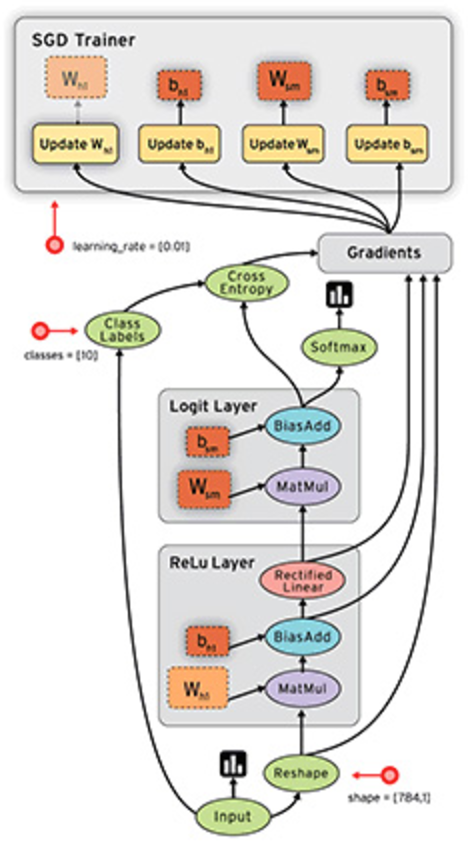
\includegraphics[width=0.4\textwidth]{figures/tf-dataflow.png}
\caption{TensorFlow数据流图}
 \label{fig:tf-dataflow}
\end{figure}

\end{content}

\subsubsection{设计原则}

\begin{content}

\begin{enum}
  \eitem{延迟计算:图的构造与执行分离,并推迟计算图的执行过程;}
  \eitem{原子\ascii{OP}:\ascii{OP}是最小的抽象计算单元,支持构造复杂的网络模型;} 
  \eitem{抽象设备:支持\ascii{CPU, GPU, TPU}多种异构计算设备类型;}
  \eitem{抽象任务:基于\ascii{Task}的\ascii{PS}任务,对新的优化算法和网络模型具有良好的可扩展性。}  
\end{enum}

\end{content}

\subsubsection{优势}

\begin{content}

相对于其他机器学习框架,\ascii{TensorFlow}具有如下方面的优势。

\begin{enum}
  \eitem{跨平台:支持多\ascii{CPU/GPU/TPU}运算;支持台式机/服务器/移动设备;支持\ascii{Windows,Linux,MacOS};}
  \eitem{分布式:支持本地和分布式的模型训练和推理;}
  \eitem{多语言:支持\ascii{Python, C++, Java, Go}等多种程序设计语言的\ascii{API};}  
  \eitem{通用性:支持各种复杂的网络模型的设计和实现;}
  \eitem{可扩展:支持\ascii{OP}扩展,\ascii{Kernel}扩展,\ascii{Device}扩展;}
  \eitem{可视化:使用\ascii{TensorBoard}可视化整个训练过程,包括计算图。}
\end{enum}

\end{content}

\section{社区发展}

\begin{content}

\tf{}是目前最为流行的机器学习框架。自开源以来,\tf{}社区相当活跃。来自众多的非\ascii{Google}员工拥有数万次代码提交,并且每周拥有近百个\ascii{Issue}被提交;在\ascii{Stack Overflow}上也拥有上万个关于\tf{}的问题被回答;在各类技术大会上,\tf{}也是一颗闪亮的明星,得到众多开发者的青睐。

\end{content}

\subsection{开源}

\begin{content}

\ascii{2015.11},\ascii{Google Research}发布文章:\href{https://research.googleblog.com/2015/11/tensorflow-googles-latest-machine\_9.html}{TensorFlow: Google's latest machine learning system, open sourced for everyone},正式宣布新一代机器学习系统\ascii{TensorFlow}开源。

随后,\ascii{TensorFlow}在\ascii{Github}上代码仓库短时间内获得了大量的\ascii{Star}和\ascii{Fork}。如\refig{tf-commits}所示,\ascii{TensorFlow}的社区活跃度已远远超过其他竞争对手,逐渐成为目前最为炙手可热的机器学习和深度学习框架,已然成为事实上的工业标准。

\begin{figure}[!htbp]
\centering
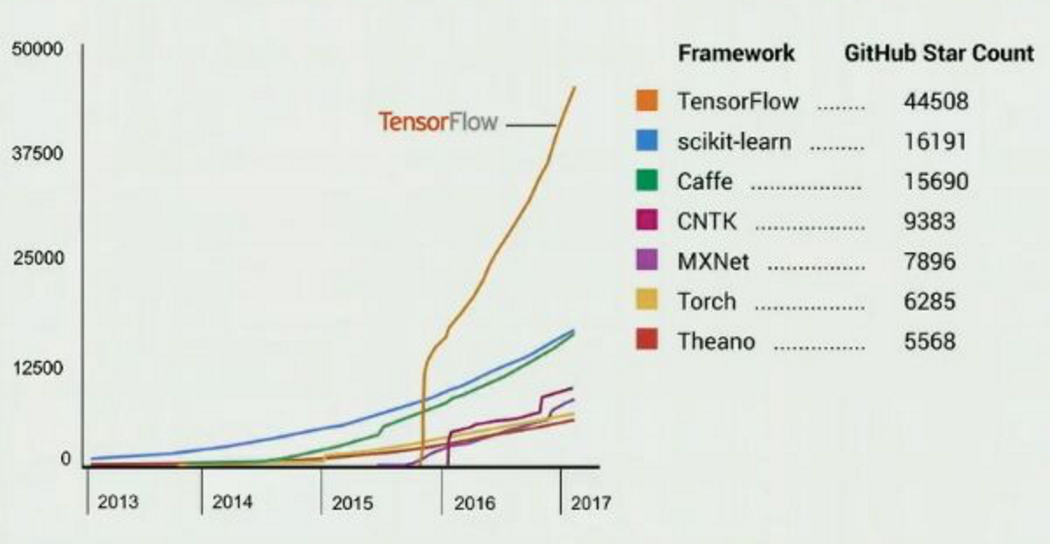
\includegraphics[width=1.0\textwidth]{figures/tf-commits.png}
\caption{TensorFlow社区活跃度}
 \label{fig:tf-commits}
\end{figure}

毫无疑问,\ascii{TensorFlow}的开源对学术界和工业界产生了巨大的影响,其极大地降低了深度学习在各个行业中应用的难度。众多的学者,工程师,企业,组织纷纷地投入到了\ascii{TensorFlow}社区,并一起完善和改进\ascii{TensorFlow},推动其不断地向前演进和发展。

\end{content}

\subsection{里程碑}

\begin{content}

\tf{}自\ascii{2015.11}开源依赖,平均一个多月发布一个版本。如\refig{tf-versions}所示,展示了\tf{}几个重要特性的发布时间。

\begin{figure}[!htbp]
\centering
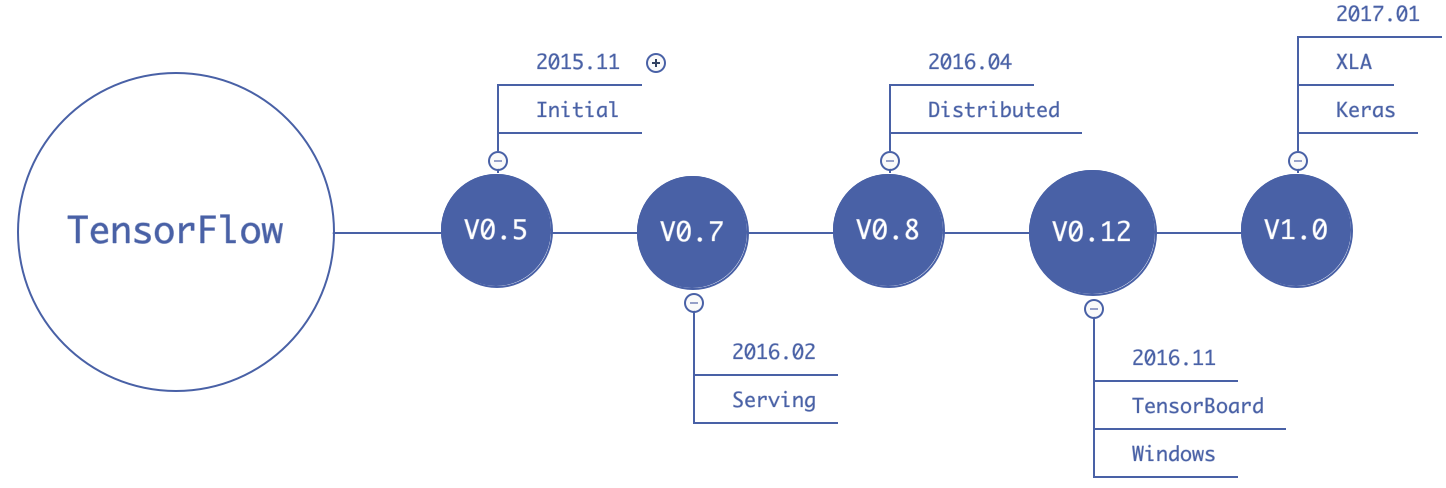
\includegraphics[width=1.0\textwidth]{figures/tf-versions.png}
\caption{TensorFlow重要里程碑}
 \label{fig:tf-versions}
\end{figure}

\end{content}

\subsection{工业应用}

\begin{content}

\ascii{TensorFlow}自开源发展一年多以来,在生产环境中被大量应用使用。在医疗方面,使用\ascii{TensorFlow}构建机器学习模型,帮助医生预测皮肤癌;在音乐、绘画领域,使用\ascii{TensorFlow}构建深度学习模型,帮助人类更好地理解艺术;在移动端,多款移动设备搭载\ascii{TensorFlow}训练的机器学习模型,用于翻译等工作。

如\refig{tf-google-apps}所示,\ascii{TensorFlow}在\ascii{Google}内部项目应用的增长也十分迅速,多个产品都有相关应用,包括:\ascii{Search, Gmail, Translate,  Maps}等等。

\begin{figure}[!htbp]
\centering
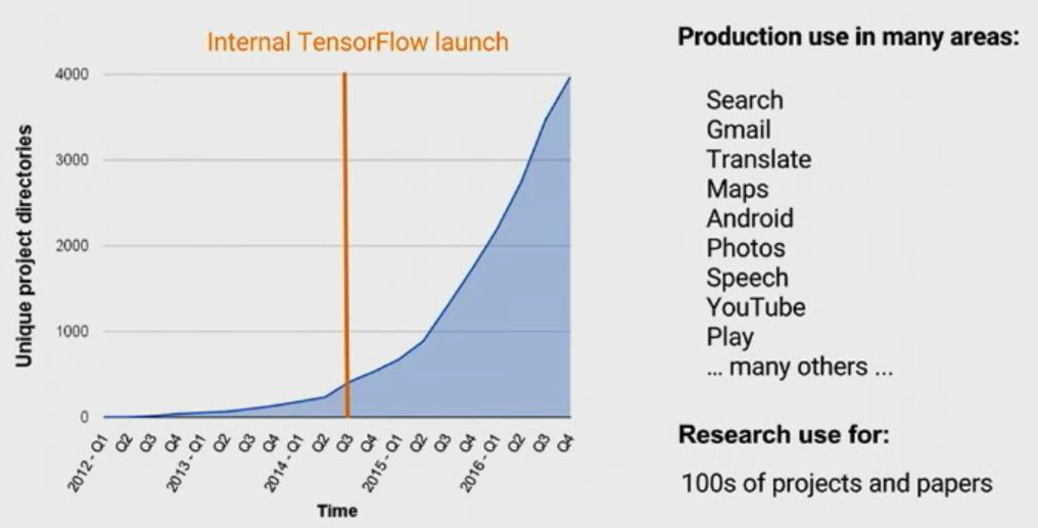
\includegraphics[width=1.0\textwidth]{figures/tf-google-apps.png}
\caption{TensorFlow在Google内部使用情况}
 \label{fig:tf-google-apps}
\end{figure}


\end{content}
% \begin{savequote}[45mm]
\ascii{Any fool can write code that a computer can understand. Good programmers write code that humans can understand.}
\qauthor{\ascii{- Martin Flower}}
\end{savequote}

\chapter{编程环境} 
\label{ch:prog-env}

\begin{content}

为了实现\tf{}的快速入门,本章将介绍\tf{}的编程环境,包括代码结构,工程构建,以便对\tf{}的系统架构建立基本的感性认识。

\end{content}

\section{代码结构}

\begin{content}

\subsection{克隆源码}

首先,从\ascii{Github}上克隆\tf{}的源代码。


\begin{leftbar}
\begin{python}
$ git clone git@github.com:tensorflow/tensorflow.git
\end{python}
\end{leftbar}

然后,切换到最新的稳定分支上。例如,\code{r1.3}分支。

\begin{leftbar}
\begin{python}
$ cd tensorflow
$ git checkout r1.3
\end{python}
\end{leftbar}

\subsection{源码结构}

运行如下命令,打印出\tf{}源码的组织结构。

\begin{leftbar}
\begin{python}[]
$ tree -d -L 1 ./tensorflow
\end{python}
\end{leftbar}

其中,本书将重点关注\code{core, python}组件,部分涉及\code{c, cc, stream\_executor}组件。

\begin{leftbar}
\begin{c++}[caption={TensorFlow源码结构}]
./tensorflow
├── c
├── cc
├── compiler
├── contrib
├── core
├── docs_src
├── examples
├── g3doc
├── go
├── java
├── python
├── stream_executor
├── tools
└── user_ops
\end{c++}
\end{leftbar}

截止当前最新发布的\ascii{1.3}版本,\tf{}代码库拥有大约\ascii{100}万代码。其中,包括\ascii{53}万行\ascii{C/C++}代码,\ascii{37}万行\ascii{Python}代码,而且在不断膨胀之中。因此,可以推测\ascii{Python}提供的编程接口是最完善的;相比之下,其他编程语言尚处于起步阶段。

\begin{leftbar}
\begin{python}[caption={TensorFlow代码统计}]
-------------------------------------------------------
Language             files    blank    comment    code
-------------------------------------------------------
C++                   2238    77610     68275    443099
Python                1881    92018    151807    369399
C/C++ Header          1175    27392     46215     86691
Markdown               218     8859         2     30925
CMake                   50     2183       986     16398
Go                      28     1779     13290     15003
Java                    72     1789      3111      7779
Bourne Shell           103     1487      3105      6074
Protocol Buffers        87     1313      3339      3452
Objective C++            9      227       181      1201
C                        8      157       130       941
make                     4      105       136       612
XML                     25      135       265       315
Groovy                   3       46        74       246
Maven                    5       21         4       245
DOS Batch                9       30         0       143
Dockerfile               7       41        69       133
Perl                     2       29        38       130
Bourne Again Shell       3       24        63       111
JSON                     3        0         0        23
Objective C              1       10        13        21
YAML                     1        3        24        15
-------------------------------------------------------
SUM:                  5932   215258    291127    982956
-------------------------------------------------------
\end{python}
\end{leftbar}

\subsection{Core}

内核的源码结构如下所示,主要包括平台,实用函数库,基础框架,\ascii{Protobuf}定义,本地运行时,分布式运行时,图操作,\ascii{OP}定义,以及\ascii{Kernel}实现等组成,这是本书重点剖析的组件之一,将重点挖掘基础框架中隐藏的领域模型,追踪整个运行时环境的生命周期和图操作的详细过程,并揭示常见\ascii{OP}的\ascii{Kernel}实现原理和运行机制。

\begin{leftbar}
\begin{c++}[caption={Core源码结构}]
./tensorflow/core
├── common_runtime
├── debug
├── distributed_runtime
├── example
├── framework
├── graph
├── grappler
├── kernels
├── lib
├── ops
├── platform
├── profiler
├── protobuf
├── public
├── user_ops
└── util
\end{c++}
\end{leftbar}

其中,\code{core}主要由\code{C++}实现,大约拥有\ascii{26}万行代码。

\begin{leftbar}
\begin{python}[caption={Core代码统计}]
-------------------------------------------------------
Language             files    blank   comment      code
-------------------------------------------------------
C++                   1368    44791     38968    259289
C/C++ Header           653    15040     24474     50506
Protocol Buffers        57      736      2371      1806
Markdown                11      327         0      1285
JSON                     2        0         0        18
-------------------------------------------------------
SUM:                  2091    60894     65813    312904
-------------------------------------------------------
\end{python}
\end{leftbar}

\subsection{Python}

\ascii{Python}定义和实现了\tf{}的编程模型,并对外开放\ascii{API}供程序员使用,其源码结构如下所示,这也是本书重点剖析的对象。

\begin{leftbar}
\begin{c++}[caption={Python源码结构}]
./tensorflow/python
├── client
├── debug
├── estimator
├── feature_column
├── framework
├── grappler
├── kernel_tests
├── layers
├── lib
├── ops
├── platform
├── profiler
├── saved_model
├── summary
├── tools
├── training
├── user_ops
└── util
\end{c++}
\end{leftbar}

其中,该组件由\code{Python}实现,大约有\ascii{18}万行代码。

\begin{leftbar}
\begin{python}[caption={Python代码统计}]
-------------------------------------------------------
Language            files     blank   comment      code
-------------------------------------------------------
Python                714     45769     69407    179565
C++                    20       496       506      3658
C/C++ Header           15       207       387       363
Markdown                4        48         0       200
Protocol Buffers        3        16        10        71
Bourne Shell            1        13        28        68
-------------------------------------------------------
SUM:                  757     46549     70338    183925
-------------------------------------------------------
\end{python}
\end{leftbar}

\subsection{Contrib}

\code{contrib}是第三方贡献的编程库,它也是\tf{}标准化之前的实验性编程接口,犹如\ascii{Boost}社区与\ascii{C++}标准之间的关系。当\code{contrib}的接口成熟后,便会被\tf{}标准化,并从\code{contrib}中搬迁至\code{core, python}中,并正式对外发布\ascii{API}。

\begin{leftbar}
\begin{python}[caption={Contrib源码结构}]
./tensorflow/contrib
├── android
├── batching
├── bayesflow
├── benchmark_tools
├── boosted_trees
├── cloud
├── cluster_resolver
├── cmake
├── compiler
├── copy_graph
├── crf
├── cudnn_rnn
├── data
├── decision_trees
├── deprecated
├── distributions
├── eager
├── factorization
├── ffmpeg
├── framework
├── fused_conv
├── gdr
├── graph_editor
├── grid_rnn
├── hooks
├── hvx
├── image
├── imperative
├── input_pipeline
├── integrate
├── keras
├── kernel_methods
├── labeled_tensor
├── layers
├── learn
├── legacy_seq2seq
├── linalg
├── linear_optimizer
├── lookup
├── losses
├── makefile
├── memory_stats
├── meta_graph_transform
├── metrics
├── mpi
├── nccl
├── ndlstm
├── nearest_neighbor
├── nn
├── opt
├── pi_examples
├── predictor
├── quantization
├── reduce_slice_ops
├── remote_fused_graph
├── resampler
├── rnn
├── saved_model
├── seq2seq
├── session_bundle
├── signal
├── slim
├── solvers
├── sparsemax
├── specs
├── staging
├── stat_summarizer
├── stateless
├── tensor_forest
├── tensorboard
├── testing
├── text
├── tfprof
├── timeseries
├── tpu
├── training
├── util
├── verbs
└── xla_tf_graph
\end{python}
\end{leftbar}

由于\tf{}社区相当活跃,\code{contrib}的变更相当频繁,截止\ascii{1.3}版本,大约有\ascii{23}万行代码,主要由\ascii{Python}设计和实现的编程接口,部分运行时由\ascii{C++}实现。

\begin{leftbar}
\begin{python}[caption={Contrib代码统计}]
-------------------------------------------------------
Language            files     blank   comment      code
-------------------------------------------------------
Python               1007     41436     75096    170355
C++                   201      5500      5313     32944
CMake                  48      2172       955     16358
C/C++ Header           99      1875      2867      6583
Markdown               46      1108         0      3485
Bourne Shell           18       232       386      1272
C                       7       151       118       931
Protocol Buffers       20       224       454       680
make                    4       105       136       612
Java                    2        77       209       335
Groovy                  1        10        20        75
Bourne Again Shell      1         6        15        59
Dockerfile              1         2         1        14
XML                     2         3         0         9
-------------------------------------------------------
SUM:                 1457     52901     85570    233712
-------------------------------------------------------
\end{python}
\end{leftbar}

\subsection{StreamExecutor}

\ascii{StreamExecutor}是\ascii{Google}另一个开源组件库,它提供了主机端(\ascii{host-side})的编程模型和运行时环境,实现了对\ascii{CUDA}和\ascii{OpenCL}的统一封装。使得主机端的代码中,可以将功能相同、数据并行的内核函数无缝地部署在\code{CUDA}或\code{OpenCL}的计算设备上执行。

目前,\ascii{StreamExecutor}被大量应用于\ascii{Google}内部的\ascii{GPGPU}应用程序的运行时。其中,\tf{}运行时也包含了一个\ascii{StreamExecutor}的快照版本,用于封装\ascii{CUDA}和\code{OpenCL}的运行时,本书将简单介绍\ascii{CUDA}的编程模型和线程模型,并详细介绍\ascii{StreamExecutor}的系统架构与工作原理,揭示\ascii{Kernel}一般的实现模式和习惯用法。

\begin{leftbar}
\begin{c++}[caption={StreamExecutor源码结构}]
./tensorflow/stream_executor
├── cuda
├── host
├── lib
└── platform
\end{c++}
\end{leftbar}

其中,\ascii{StreamExecutor}使用\code{C++}实现,大约有\ascii{2.5}万行代码。

\begin{leftbar}
\begin{python}[caption={StreamExecutor代码统计}]
-------------------------------------------------------
Language            files     blank   comment      code
-------------------------------------------------------
C++                    43      2440      1196     16577
C/C++ Header           81      2322      5080      8625
-------------------------------------------------------
SUM:                  124      4762      6276     25202
-------------------------------------------------------
\end{python}
\end{leftbar}

\subsection{Compiler}

众所周知,灵活性是\tf{}最重要的设计目标和核心优势,因此\tf{}的系统架构具有良好的可扩展性。\tf{}可用于定义任意图结构,并使用异构的计算设备有效地执行。但是,熊掌与鱼翅不可兼得,当低级\code{OP}组合为计算子图时,并期望在\code{GPU}上有效执行时,运行时将启动更多的\code{Kernel}的运算。

因此,\tf{}分解和组合\code{OP}的方法,在运行时并不能保证以最有效的方式运行。此时,\ascii{XLA}技术孕育而生,它使用\ascii{JIT}编译技术来分析运行时的计算图,它将多个\code{OP}融合在一起,并生成更高效的本地机器代码,提升计算图的执行效率。

\begin{leftbar}
\begin{python}[caption={Compiler源码结构}]
./tensorflow/compiler
├── aot
├── jit
├── plugin
├── tests
├── tf2xla
└── xla
\end{python}
\end{leftbar}

\ascii{XLA}技术目前处于初级的研发阶段,是\tf{}社区较为活跃研究方向,截止目前代码规模大约为\ascii{12.5}万行,主要使用\ascii{C++}实现。

\begin{leftbar}
\begin{python}[caption={Compiler代码统计}]
-------------------------------------------------------
Language            files     blank   comment      code
-------------------------------------------------------
C++                   455     19010     18334    102537
C/C++ Header          250      5939     10323     15510
Python                 37      1255      1416      6446
Protocol Buffers        5       312       501       781
Markdown                2         0         0         3
-------------------------------------------------------
SUM:                  749     26516     30574    125277
-------------------------------------------------------
\end{python}
\end{leftbar}

\end{content}

\section{工程构建}

\begin{content}

在开始之前,尝试\tf{}源码的构建过程,了解\tf{}的基本构建方式、工具,及其依赖的组件库、及其第三方工具包,对于理解\tf{}工作原理具有很大的帮助。但是,因篇幅受限,本章仅以\ascii{Mac OS}为例,讲述\tf{}的源码编译、安装、及其验证过程。其他操作系统,请查阅\tf{}的官方文档。

\subsection{环境准备}

\ascii{TensorFlow}的前端是一个支持多语言的编程接口。因此,编译\ascii{TensorFlow}源代码之前,需要事先安装相关的编译器、解释器、及其运行时环境。例如,使用\ascii{Python}作为编程接口,需要事先安装\ascii{Python}解释器。

其次,在构建系统之前,也需要事先安装\ascii{GCC}或\ascii{Clang}等\ascii{C++}编译器,用于编译后端系统实现。另外,\ascii{TensorFlow}使用\ascii{Bazel}的构建工具,是一个更高抽象的\ascii{Make}工具。不幸的是,\ascii{Bazel}依赖于\ascii{JDK},因此在安装\ascii{Bazel}之前,还得需要事先安装\ascii{JDK}。

\subsubsection{安装JDK}

推荐从\ascii{Oracle}官网上下载\ascii{1.8}及以上版本的\ascii{JDK},然后配置相关环境变量。

\begin{leftbar}
\begin{python}
$ sudo mkdir -p /usr/lib/jvm
$ sudo tar zxvf jdk-8u51-linux-x64.tar.gz -C /usr/lib/jvm
$ sudo ln -s /usr/java/jdk1.8.0_51 /usr/java/default
\end{python}
\end{leftbar}

创建\ascii{Java}相关的环境变量,并将其添加到\code{~/.bashrc}的配置文件中。

\begin{leftbar}
\begin{python}
$ echo 'export JAVA_HOME=/usr/java/default' >> ~/.bashrc
$ echo 'export PATH="$JAVA_HOME/bin:$PATH"' >> ~/.bashrc
\end{python}
\end{leftbar}

\subsubsection{安装Bazel}

在\ascii{Mac OS}上,可以使用\ascii{brew}安装\ascii{Bazel}。

\begin{leftbar}
\begin{python}
$ brew install bazel
\end{python}
\end{leftbar}

如果系统未安装\ascii{brew},可以执行如下命令先安装\ascii{brew}。当然,安装\ascii{brew}需要事先安装\ascii{Ruby}解释器,在此不再冗述。

\begin{leftbar}
\begin{python}
$ /usr/bin/ruby -e "$(curl -fsSL https://raw.githubusercontent.com/Homebrew/install/master/install)"
\end{python}
\end{leftbar}

\subsubsection{安装Swig}

\ascii{TensorFlow}使用\ascii{Swig}构建多语言的编程环境,自动生成相关的包装器。因此,在构建之前需要事先安装\ascii{Swig}的工具包。

\begin{leftbar}
\begin{python}
$ brew install swig
\end{python}
\end{leftbar}

\subsubsection{安装Python依赖包}

使用\ascii{pip}安装\ascii{TensorFlow}所依赖的\ascii{Python}包。

\begin{leftbar}
\begin{python}
$ sudo pip install six numpy wheel autograd
\end{python}
\end{leftbar}

如果系统未安装\ascii{pip},则可以使用\ascii{brew}先安装\ascii{pip}。

\begin{leftbar}
\begin{python}
$ brew install pip
\end{python}
\end{leftbar}

\subsubsection{安装CUDA工具包}

当系统安装了\ascii{CUDA}计算兼容性大于或等于\ascii{3.0}的\ascii{GPU}卡时,则需要安装\ascii{CUDA工具包, cuDNN},实现\tf{}运行时的\ascii{GPU}加速。推荐从\ascii{NVIDIA}官网上下载\ascii{CUDA Toolkit 8}及以上版本,并安装到系统中,配置相关环境变量。

\begin{leftbar}
\begin{python}
$ echo 'export CUDA_HOME=/usr/local/cuda' >> ~/.bashrc
$ echo 'export LD_LIBRARY_PATH=$CUDA_HOME/lib:$LD_LIBRARY_PATH' >> ~/.bashrc
\end{python}
\end{leftbar}

然后,再下载\ascii{cuDNN 5.1}及以上版本,并将其解压至\code{CUDA\_HOME}相关系统目录中。

\begin{leftbar}
\begin{python}
$ sudo tar -xvf cudnn-8.0-macos-x64-v5.1.tgz -C /usr/local
\end{python}
\end{leftbar}

\subsection{配置}

至此,编译环境一切就绪,执行\code{./configure}配置\ascii{TensorFlow}的编译环境了。特殊地,当系统支持\ascii{GPU},则需要配置相关的\ascii{CUDA/cuDNN}编译环境。

\begin{leftbar}
\begin{python}
$ ./configure
\end{python}
\end{leftbar}

\subsection{构建}

当配置成功后,使用\ascii{Bazel}启动\ascii{TensorFlow}的编译。

\begin{leftbar}
\begin{python}
$ bazel build --config=opt //tensorflow/tools/pip_package:build_pip_package
\end{python}
\end{leftbar}

特殊地,当支持\ascii{GPU}计算时,添加\code{--config=cuda}编译选项。

\begin{leftbar}
\begin{python}
$ bazel build -c opt --config=cuda //tensorflow/tools/pip_package:build_pip_package
\end{python}
\end{leftbar}

编译成功后,便可以构建\ascii{TensorFlow}的\ascii{Wheel}包。

\begin{leftbar}
\begin{python}
$ bazel-bin/tensorflow/tools/pip_package/build_pip_package /tmp/tensorflow_pkg
\end{python}
\end{leftbar}

\subsection{安装}

当\ascii{Whell}包构建成功后,使用\ascii{pip}安装\ascii{TensorFlow}到系统中。

\begin{leftbar}
\begin{python}
$ sudo pip install /tmp/tensorflow_pkg/tensorflow-1.2.0-py2-none-any.whl
\end{python}
\end{leftbar}

\subsection{验证}

启动\ascii{Python}解释器,验证\ascii{TensorFlow}安装是否成功。

\begin{leftbar}
\begin{python}
$ python
>>> import tensorflow as tf
>>> hello = tf.constant('Hello, TensorFlow!')
>>> sess = tf.Session()
>>> print(sess.run(hello))
Hello, TensorFlow!
\end{python}
\end{leftbar}

\subsection{配置IDE}

在阅读代码之前,选择一个适宜的\ascii{IDE}可以改善代码阅读的质量和速度。作者推荐使用\ascii{Eclipse CDT}阅读\ascii{C++}代码,使用\ascii{PyCharm}阅读\ascii{Python}代码。当阅读\code{Python}时,导入\tf{}源代码到\ascii{PyCharm}即可,在此不再冗述。但是,当阅读\ascii{C++}代码时,需要配置\ascii{TensorFlow, CUDA, Eigen3}头文件的搜索目录,并添加相关预定义的宏,以便\code{CDT}正确解析代码中的符号。

\subsubsection{创建Eclipse工程}

创建一个\ascii{Eclipse C++}工程,如\refig{setup-eclipse}所示。确定唯一的项目名称,手动地指定\ascii{TensorFlow}源代码的根目录,并选择\ascii{Makefile}的空工程。然后,按照\ascii{Properties > C/C++ General > Paths and Symbols > Includes}配置头文件的搜索目录。

\begin{table}[!htbl]
\resizebox{0.95\textwidth}{!} {
\begin{tabular*}{1.2\textwidth}{@{}ll@{}}
\toprule
\ascii{配置项} & \ascii{目录} \\
\midrule
\ascii{TensorFlow} & \code{/usr/local/lib/python2.7/site-packages/tensorflow/include} \\
\ascii{CUDA} & \code{/usr/local/cuda/include} \\ 
\bottomrule
\end{tabular*}
}
\caption{头文件搜索目录}
\label{tbl:tf-includes}
\end{table}

\begin{figure}[!htbl]
\centering
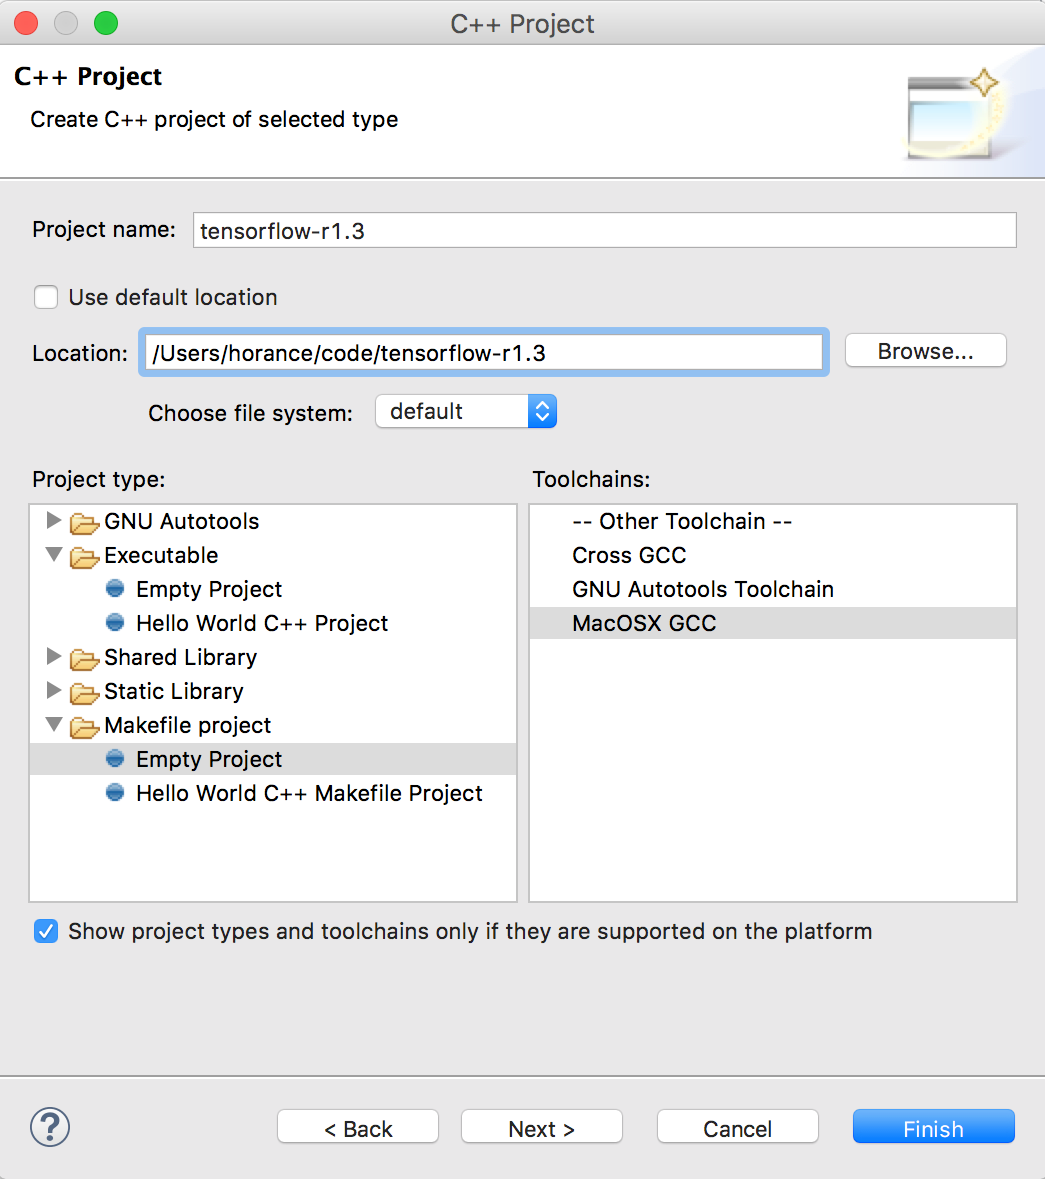
\includegraphics[width=0.75\textwidth]{figures/setup-eclipse.png}
\caption{创建Eclipse C++工程}}
 \label{fig:setup-eclipse}
\end{figure}

\subsubsection{配置Eigen}

不幸的是,\ascii{Eigen}对外公开的头文件缺少\code{.h}的后缀名,\code{CDT}无法解析相关的符号。请参阅\code{\href{http://eigen.tuxfamily.org/index.php?title=IDEs}{http://eigen.tuxfamily.org/index.php?title=IDEs}}相关说明,按照\ascii{Preferences > C/C++ > Coding Style > Organize Includes > Header Substitution}导入\code{eigen-header-substitution.xml}文件,如\refig{eclipse-eigen3}所示。

\begin{figure}[!htbl]
\centering
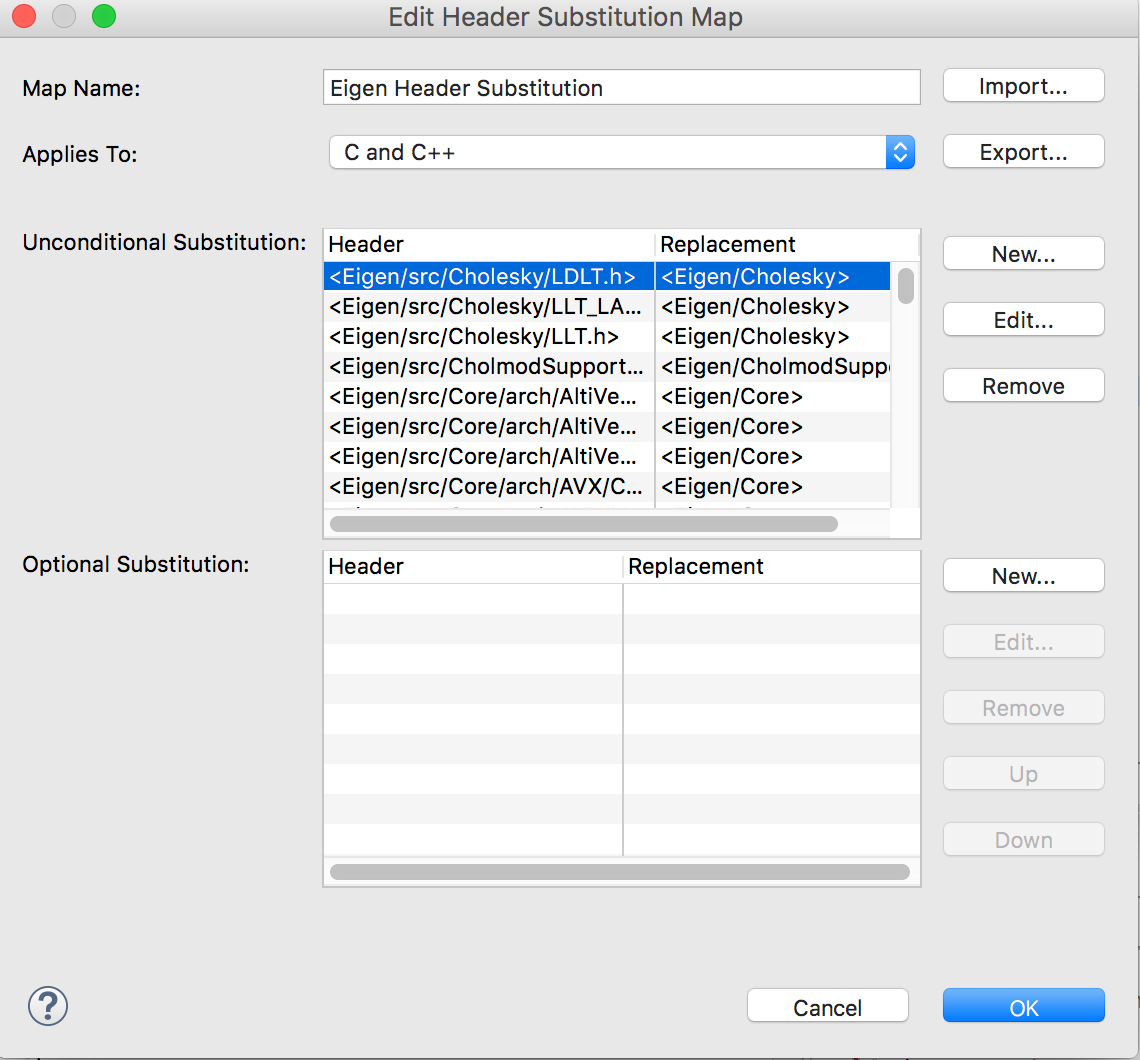
\includegraphics[width=0.75\textwidth]{figures/eclipse-eigen3.png}
\caption{替换\ascii{Eigen}的头文件}
 \label{fig:eclipse-eigen3}
\end{figure}

\end{content}

\section{技术栈}

\begin{content}

如\refig{tf-stack}所示,按照系统的层次结构展示了\tf{}的技术栈,构成了\tf{}生态系统的核心。

\begin{figure}[H]
\centering
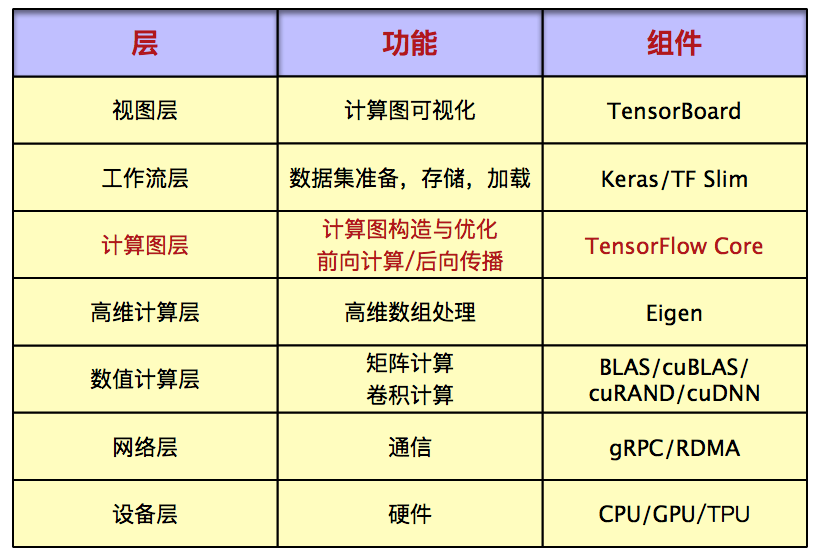
\includegraphics[width=0.7\textwidth]{figures/tf-stack.png}
\caption{TensorFlow技术栈}}
 \label{fig:tf-stack}
\end{figure}

\end{content}

% \begin{savequote}[45mm]
\ascii{Any fool can write code that a computer can understand. Good programmers write code that humans can understand.}
\qauthor{\ascii{- Martin Flower}}
\end{savequote}

\chapter{破冰之旅} 
\label{ch:ice-breaker}

\begin{content}

在开始探究\tf{}内核之前,亲自动手实践模型的训练,熟悉模型训练的基本方法和调优技术,对于理解后续章节的内容将大有裨益。\footnote{ 本章内容摘自\ascii{Martin G\"{o}rner}在\ascii{Codelabs}上发表的文章:\href{https://codelabs.developers.google.com/codelabs/cloud-tensorflow-mnist}{Tensorflow and deep learning, without a PhD},经由\ascii{Martin G\"{o}rner}同意,授权该文章在本书中发表。}

通过本文学习和实践,将了解到如何构建并训练出能够识别手写数字的神经网络。首先,尝试使用单层感知器模型,然后尝试使用多层感知器模型,最后尝试使用卷积神经网络。并在训练过程中,介绍了算法调优的一些常用技术,包括选择更好的激活函数,学习速率衰减,实施\ascii{Dropout}技术等;最终,将模型的准确率提升至\ascii{99%}以上。

在介绍每一种网络模型之前,将简单给出该模型的算法理论知识,帮助大家更好地理解程序的内容。但是,本书不是专业介绍算法的书籍,如需了解更多相关算法内容,请查阅相关文献或论文。

\end{content}

\section{问题提出}

\begin{content}

本章使用\ascii{MNIST}数据集完成手写数字的网络模型训练,它包含了\ascii{60000}个训练样本数据;其中,包括\ascii{10000}个测试样本数据。

如\refig{mnist-x}所示,对于任意一个样本数据$x$,使用$28 \times 28$像素的数字矩阵表示。为了简化,将$28 \times 28$的矩阵实施扁平化处理,得到长度为\ascii{784}的一维向量。

\begin{figure}[H]
\centering
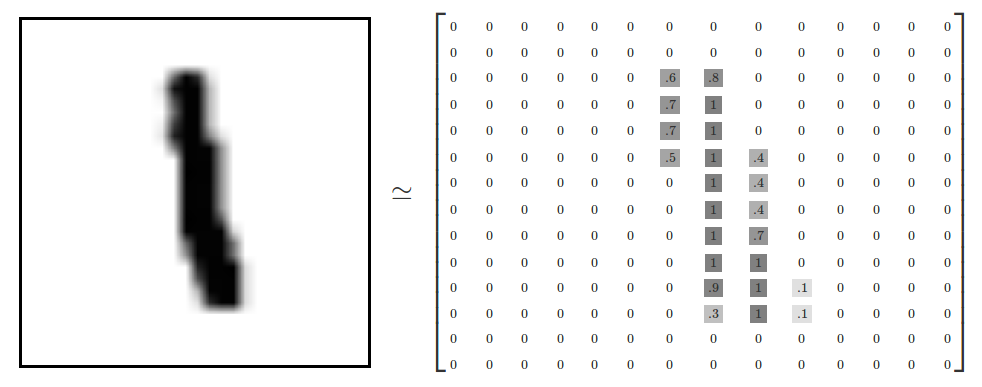
\includegraphics[width=0.9\textwidth]{figures/mnist-x.png}
\caption{MNIST样本数据表示}
 \label{fig:mnist-x}
\end{figure}

因此,在\ascii{MNIST}训练数据集中,\code{mnist.train.images}是一个\code{[60000, 784]}的二维矩阵。其中,矩阵中每一个元素,表示图片中某个像素的强度值,其值介于\ascii{0}和\ascii{1}之间。如\refig{mnist-train-xs}所示。

\begin{figure}[H]
\centering
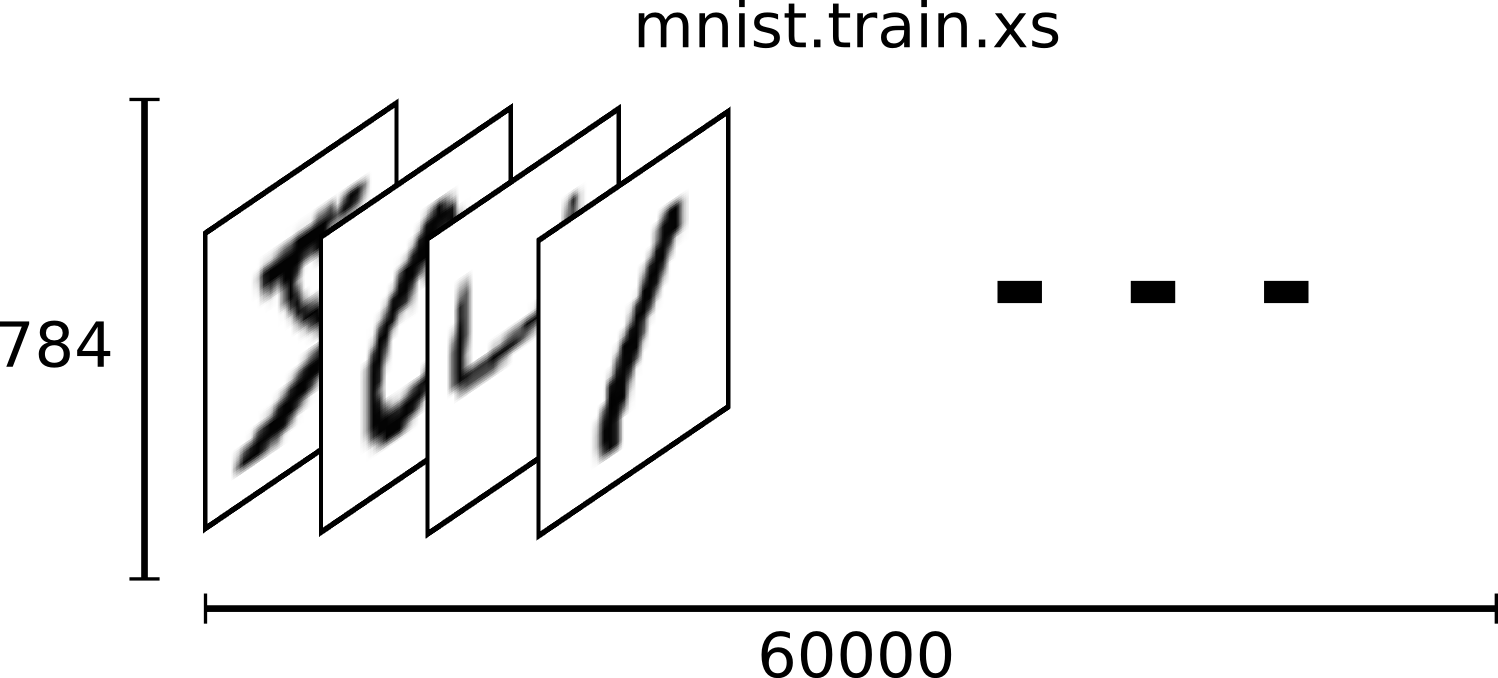
\includegraphics[width=0.9\textwidth]{figures/mnist-train-xs.png}
\caption{MNIST训练数据集:输入数据集}
 \label{fig:mnist-train-xs}
\end{figure}

相对应地,\ascii{MNIST}数据集的标签是介于\ascii{0}到\ascii{9}的数字,\code{mnist.train.labels}是一个\code{[60000, 10]}的二维矩阵,其中每一行是一个\ascii{\quo{one-hot}}向量。如\refig{mnist-train-ys}所示。

\begin{figure}[H]
\centering
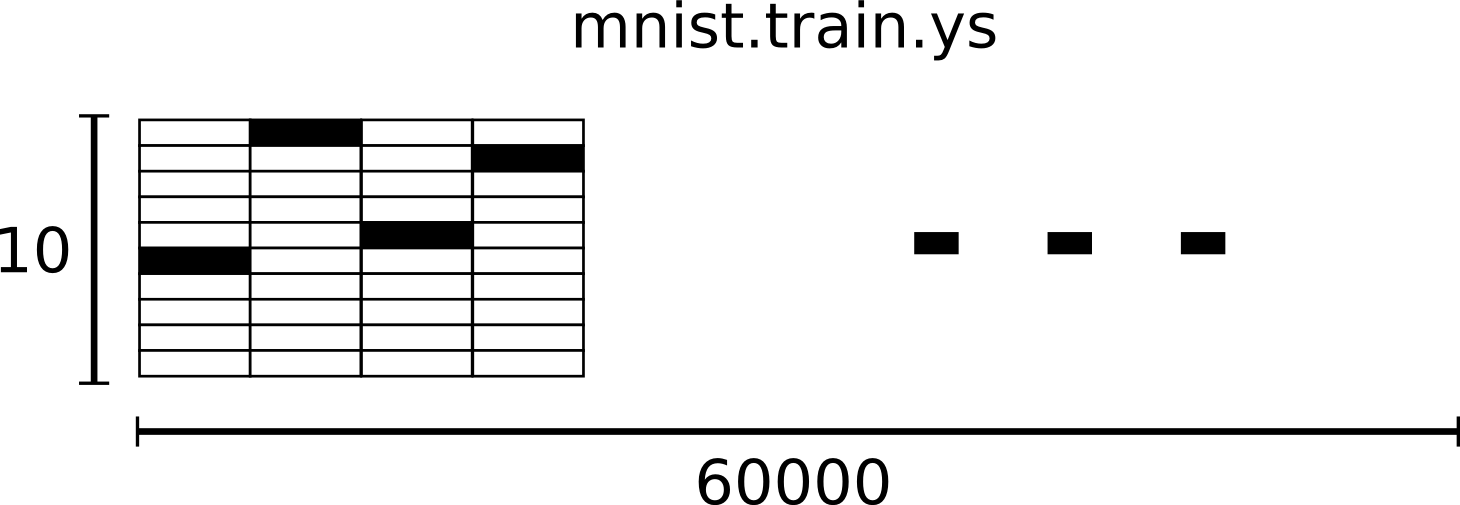
\includegraphics[width=0.9\textwidth]{figures/mnist-train-ys.png}
\caption{MNIST训练数据集:标签数据集}
 \label{fig:mnist-train-ys}
\end{figure}

\end{content}

\section{图示说明}

\begin{content}

为了更好地可视化整个训练过程,使用\ascii{matplotlib}工具包绘制了\ascii{5}种类型的画板。如\refig{mnist-training-digits}所示,表示\code{batch\_size = 100}时,一个\ascii{mini-batch}的训练样本数据集。其中,白色背景表示数字被正确识别;而红色背景表示数字被误分类,手写数字的左侧标识了正确的标签值,而右侧标识了错误的预测值。

\ascii{MNIST}拥有\ascii{50000}个训练样本,如果\code{batch\_size}为\ascii{100},则需要迭代\ascii{500}次才能完整地遍历一次训练样本数据集,常称为一个\ascii{epoch}周期。

\begin{figure}[H]
\centering
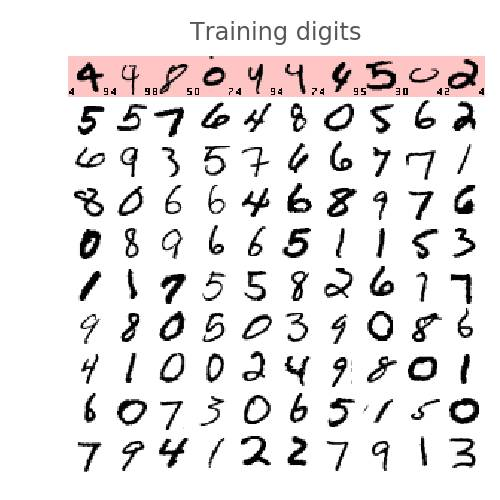
\includegraphics[width=0.6\textwidth]{figures/mnist-training-digits.jpeg}
\caption{一次mini-batch的训练样本数据集,其中\code{batch\_size=100}}
 \label{fig:mnist-training-digits}
\end{figure}

如\refig{mnist-test-digits}所示,\ascii{MNIST}使用了规模为\ascii{10000}的测试样本数据集测试模型的当前精度。其中,左侧表示目前模型的大致精度;同样地,白色背景表示数字被正确识别;而红色背景表示数字被误分类,手写数字的左侧标识了正确的标签值,而右侧标识了错误的预测值。

\begin{figure}[H]
\centering
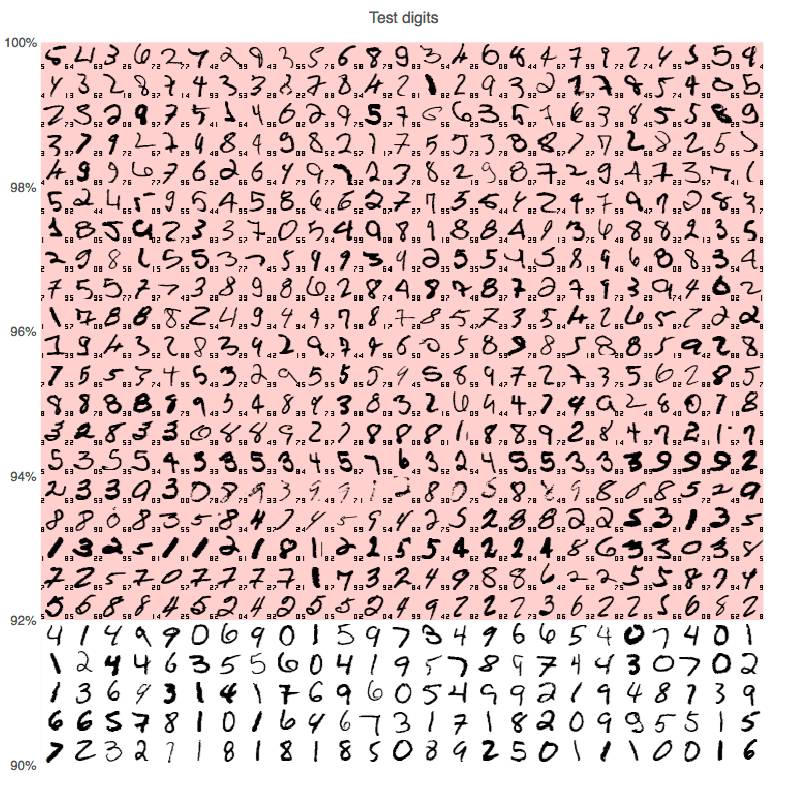
\includegraphics[width=0.6\textwidth]{figures/mnist-test-digits.jpeg}
\caption{当前的模型精度:基于测试样本数据集}
 \label{fig:mnist-test-digits}
\end{figure}

如\refig{mnist-cross-entropy-loss-fig}所示,使用交叉熵函数量化预测值与标签值之前的误差。其中,\ascii{x}轴表示迭代的次数,\ascii{y}轴表示损失值。另外,基于训练样本数据集,损失值的曲线抖动较大;而基于测试样本数据集,损失值的曲线抖动较小。

\begin{figure}[H]
\centering
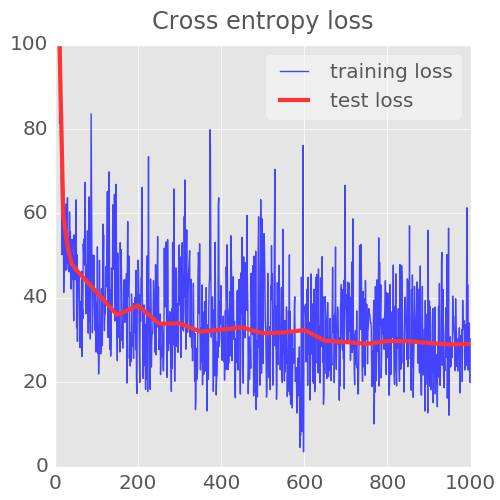
\includegraphics[width=0.6\textwidth]{figures/mnist-cross-entropy-loss-fig.jpeg}
\caption{训练和测试的交叉熵损失}
 \label{fig:mnist-cross-entropy-loss-fig}
\end{figure}

如\refig{mnist-accuracy-fig}所示,可以实时计算得到模型在当前训练数据集和测试集上的精度。其中,\ascii{x}轴表示迭代的次数,\ascii{y}轴表示精度值。另外,基于训练样本数据集,精度曲线抖动较大;而基于测试样本数据集,精度曲线抖动较小。

\begin{figure}[H]
\centering
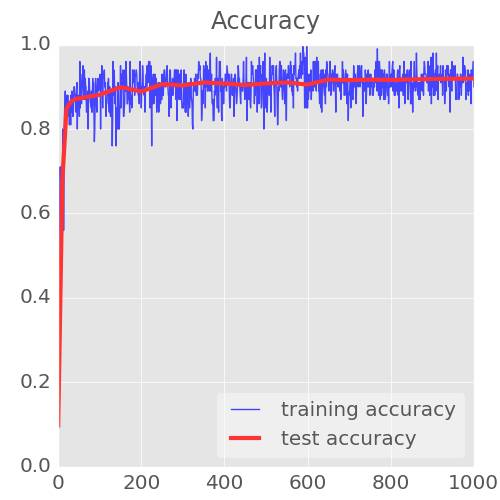
\includegraphics[width=0.6\textwidth]{figures/mnist-accuracy-fig.jpeg}
\caption{训练和测试的精度}
 \label{fig:mnist-accuracy-fig}
\end{figure}

如\refig{mnist-weight-fig}所示,对于模型的每一个训练参数(包括偏置),可以统计得到其对应的数值分布图。当模型不能收敛时,参数的数值分布图能够给出有帮助的提示信息。

\begin{figure}[H]
\centering
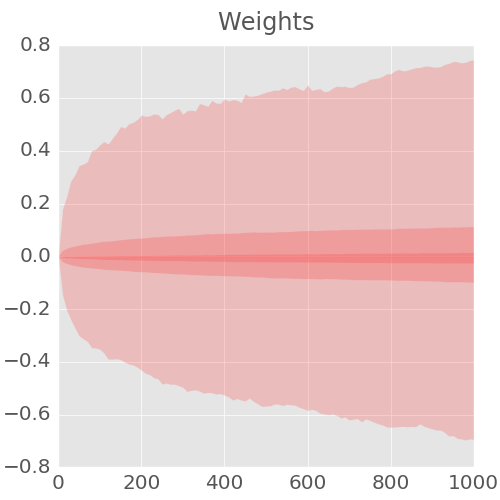
\includegraphics[width=0.6\textwidth]{figures/mnist-weight-fig.png}
\caption{权重分布图}
 \label{fig:mnist-weight-fig}
\end{figure}

\end{content}

\section{单层感知器}

\begin{content}

首先,尝试构建\ascii{10}个神经元的单层感知器。如\refig{mnist-slp}所示,对于诸如手写数字识别的多分类问题,理论上常使用\ascii{softmax}的激活函数。

\begin{figure}[H]
\centering
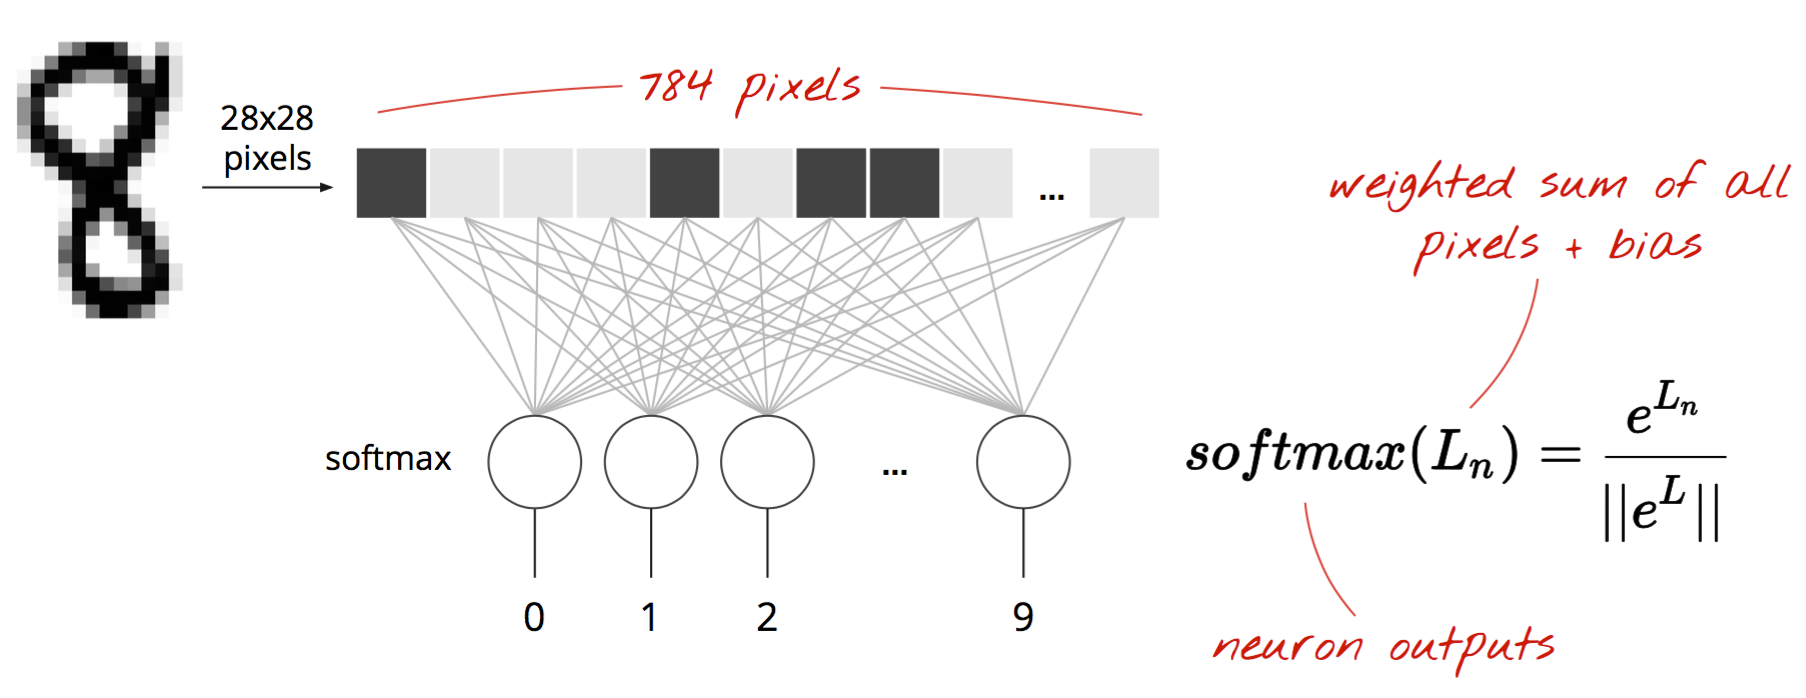
\includegraphics[width=0.8\textwidth]{figures/mnist-slp.png}
\caption{单层感知器}
 \label{fig:mnist-slp}
\end{figure}

\subsection{理论基础}

理论上,\ascii{softmax}回归是\ascii{logistic}回归的广义扩展。其中,\ascii{logistic}回归是为了解决二分类问题,即$y \in \{ 0,1\}$;而\ascii{softmax}回归是为了解决$ k $分类问题,即$y \in \{ 1,2,...,k\}$。

\subsubsection{符号定义}

为了形式化地描述\ascii{softmax}回归问题,此处定义了一些常用符号。

 \begin{itemize}
   \item \ascii{训练样本集}: $ S = \{ ({x^{(i)}},{y^{(i)}});i = 1,2,...,m\} $
   \item \ascii{第$i$个训练样本}: $ ({x^{(i)}},{y^{(i)}}) $
   \item \ascii{样本输入}: $ x = ({x_1},{x_2},...,{x_n})^{T}  \in {\mathbb{R}^n} $
   \item \ascii{样本标签(one-hot)}: $ y = ({y_1},{y_2},...,{y_k})^{T} \in {\mathbb{R}^k} $
   \item \ascii{权重}: $ W \in {\mathbb{R}^{n \times k}} $   
   \item \ascii{偏置}: $ b \in {\mathbb{R}^k} $   
   \item \ascii{softmax函数}: $ 
softmax {(z_i)} = \tfrac{{{e^{{z_i}}}}}{{\sum\limits_{j = 1}^k {{e^{{z_j}}}} }}  \quad i = 1,2,...,k
$
 \end{itemize}

\subsubsection{softmax函数}

如\refig{softmax}所示,模型先求取线性加权和$z$,然后求取$e^z$,最后再实施归一化操作。

\begin{figure}[H]
\centering
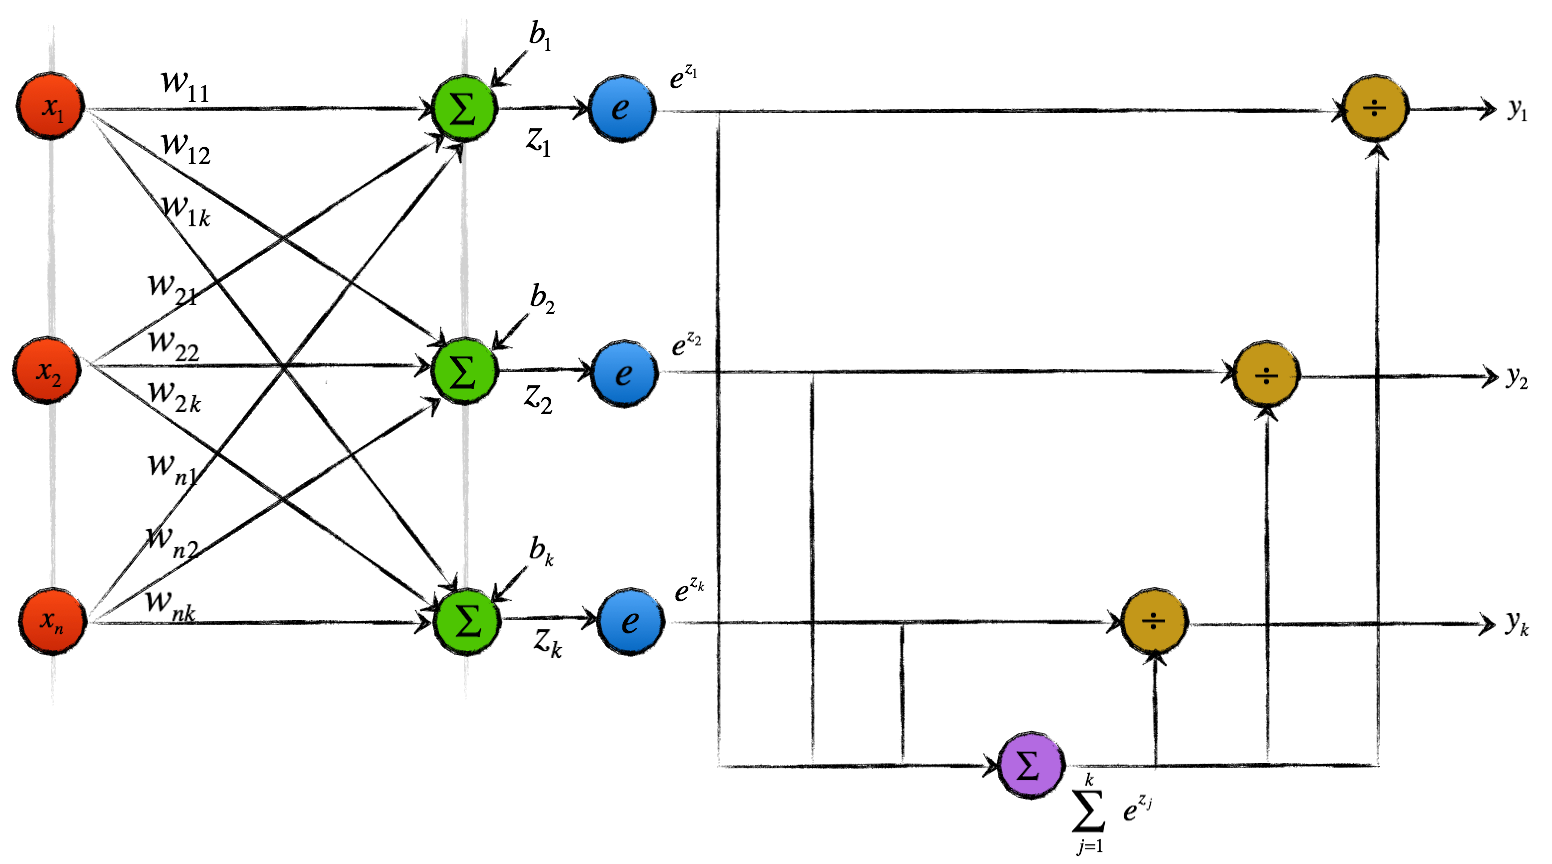
\includegraphics[width=0.8\textwidth]{figures/softmax.png}
\caption{softmax函数}
 \label{fig:softmax}
\end{figure}

\subsubsection{权重与偏置}

权重$W$为一个$n \times k$的二维矩阵。

\[
W = \left( {{W_1},{W_2},...,{W_k}} \right) = \left( {\begin{array}{*{20}{c}}
  {{w_{11}}}& \ldots &{{w_{1k}}} \\ 
   \vdots & \ddots & \vdots  \\ 
  {{w_{n1}}}& \cdots &{{w_{nk}}} 
\end{array}} \right) \in {\mathbb{R}^{n \times k}}
\]

其中,$W_j$是一个长度为$n$的向量。

\[
{W_j} = {\left( {{w_{1j}},{w_{2j}},...,{w_{nj}}} \right)^T} \in {\mathbb{R}^n}, j = 1,2,...,k \\
\]

而偏置$b$是一个长度为$k$的\ascii{\quo{one-hot}}向量。

\[
b = {({b_1},{b_2},...,{b_k})^T} \in {\mathbb{R}^k}
\]

\subsubsection{模型定义}

多分类问题的单层感知器模型,使用\ascii{softmax}激活函数,可以如此定义。

\[\begin{aligned}
  y =  & {h_{W,b}}(x) = softmax (z) = softmax ({W^T}x + b) \\ 
   =  & {\left( {{y_1},{y_2},...,{y_k}} \right)^T} \\ 
   =  & \frac{1}{{\sum\limits_{j = 1}^k {{e^{{z_j}}}} }}{\left( {{e^{{z_1}}},{e^{{z_2}}},...,{e^{{z_k}}}} \right)^T} \\ 
   =  & \frac{1}{{\sum\limits_{j = 1}^k {{e^{W_j^Tx + {b_j}}}} }}{\left( {{e^{W_1^Tx + {b_1}}},{e^{W_2^Tx + {b_2}}},...,{e^{W_k^Tx + {b_k}}}} \right)^T} \ 
\end{aligned} \]

其中,对于任意给定的样本$ (x, y) \in S $,$ z_i $表示$W_i^Tx+b_i$的线性加权和,而$y_i(i=1,2,...,k)$表示将其划归为类$i$的概率。

\[\begin{gathered}
  P\left( {y = i|x;W,b} \right) = \frac{{{e^{W_i^Tx + b_i}}}}{{\sum\limits_{j = 1}^k {{e^{W_j^Tx + b_j}}} }} \hfill \\
  i = 1,2,...,k \hfill \\ 
\end{gathered} \]


\subsubsection{交叉熵函数}

基于样本数据集$ S = \{ ({x^{(i)}},{y^{(i)}});i = 1,2,...,m\} $,交叉熵损失函数可以如此定义。

\[\begin{aligned}
  J(W,b) =  &  - \frac{1}{m}\sum\limits_{i = 1}^m {{y^{(i)}}\log \left( {{{\widehat y}^{(i)}}} \right)}  \\ 
   =  &  - \frac{1}{m}\sum\limits_{i = 1}^m {\sum\limits_{j = 1}^k {y_j^{(i)}\log \left( {\widehat y_j^{(i)}} \right)} }  \\
\end{aligned} \]

\ascii{softmax}多分类问题,就是求取最优解$(W^*,b^*)$,使得

\[W^*,b^* = \mathop {\arg \min }\limits_{W,b} J(W,b)\]

\subsubsection{计算梯度}

对于任意一个样本$ (x,y) \in S $,可以推导出$ J(W,b) $相对于$ W $与$ b $的梯度公式。

\[\begin{aligned}
  {\nabla _W}J\left( {W,b;x,y} \right) =  & \left( {\widehat y - y} \right)x \\ 
  {\nabla _b}J\left( {W,b;{x^{(i)}},{y^{(i)}}} \right) =  & \left( {\widehat y - y} \right) \\ 
\end{aligned} \]


\subsubsection{参数更新}

对于训练样本数据$ S $,根据$W, b$的梯度公式,完成本次迭代的参数更新。

\[\begin{aligned}
  W \leftarrow  & W - \alpha \frac{{\sum\limits_{i = 1}^m {{\nabla _W}J\left( {W,b;{x^{(i)}},{y^{(i)}}} \right)} }}{m} \\ 
  b \leftarrow  & b - \alpha \frac{{\sum\limits_{i = 1}^m {{\nabla _b}J\left( {W,b;{x^{(i)}},{y^{(i)}}} \right)} }}{m} \\ 
\end{aligned} \]

\subsection{定义模型}

接下来,使用\tf{}完成该模型的搭建和训练。需要注意的是,理论上的公式与\tf{}具体实现存在微妙的差异。理论上,公式中的$x$常表示一个样本,但\tf{}中的\code{x}常表示一个\ascii{mini-batch}的样本数据集。因此,使用\tf{}设计网络模型时,需要特别关注各个张量大小的变化是否符合预期。

\subsubsection{输入和标签}

首先,使用\code{tf.placeholder}分别定义训练样本的输入和标签。

\begin{leftbar}
\begin{python}
x = tf.placeholder(tf.float32, [None, 28, 28, 1])
t = tf.placeholder(tf.float32, [None, 10])
\end{python}
\end{leftbar}

\code{tf.placeholder}定义了一个占位的\ascii{OP}。\code{None}表示未确定的样本数目,此处表示\code{batch\_size}的大小;当\code{Session.run}时,将通过\code{feed\_dict}的字典提供一个\ascii{mini-batch}的样本数据集,从而自动推导出\code{tf.placeholder}的大小。

另外,每张图片使用$ 28 \times 28 \times 1 $的三维数据表示(灰度为\ascii{1})。为了简化问题,此处将输入的样本数据扁平化,将其变换为长度为\ascii{784}的一维向量。其中,\ascii{-1}表示\ascii{mini-batch}的样本数目,由运行时自动推演其大小。

\begin{leftbar}
\begin{python}
x = tf.reshape(x, [-1, 784])
\end{python}
\end{leftbar}

\subsubsection{定义变量}

然后,使用\code{tf.Variable}定义模型参数。定义训练参数时,必须指定参数的初始化值;训练变量将根据初始化值,自动推演数据的类型,及其大小。

\begin{leftbar}
\begin{python}
w = tf.Variable(tf.zeros([784, 10]))
b = tf.Variable(tf.zeros([10]))
\end{python}
\end{leftbar}

此外,变量在使用之前,必须完成初始化。此处,\code{init\_op}将初始化所有全局的训练参数。

\begin{leftbar}
\begin{python}
init_op = tf.global_variables_initializer()
\end{python}
\end{leftbar}

\subsubsection{模型定义}

接下来,便可以很容易地得到多分类问题的单层感知器模型。

\begin{leftbar}
\begin{python}
y = tf.nn.softmax(tf.matmul(x, w) + b)
\end{python}
\end{leftbar}

如\refig{mnist-linear-sum}所示,首先计算\code{x}与\code{w}的矩阵乘法,让后将\code{b}广播(\ascii{broadcast})到矩阵的每一行相加,最终得到训练参数的线性加权和。

\begin{figure}[H]
\centering
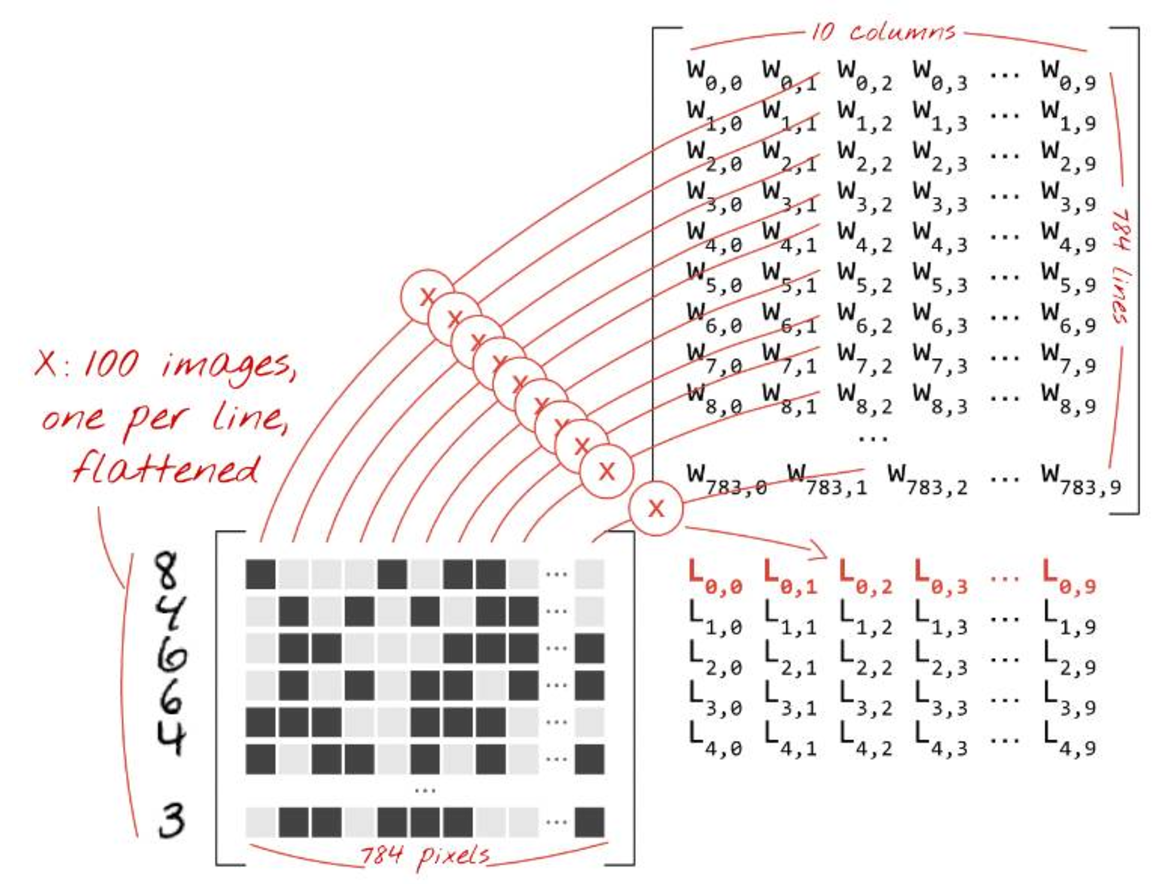
\includegraphics[width=0.8\textwidth]{figures/mnist-linear-sum.png}
\caption{线性加权和}
 \label{fig:mnist-linear-sum}
\end{figure}

如\refig{mnist-softmax}所示,\ascii{softmax}将逐行实施运算,最终,\code{y}的大小为\code{[100, 10]}。

\begin{figure}[H]
\centering
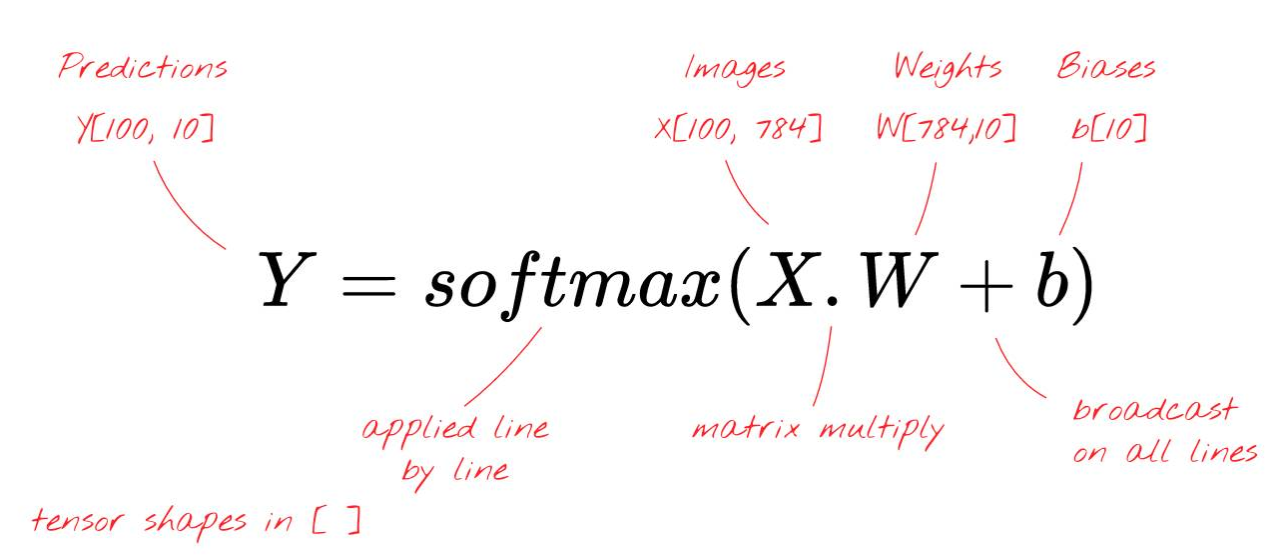
\includegraphics[width=0.8\textwidth]{figures/mnist-softmax.png}
\caption{激活函数:softmax}
 \label{fig:mnist-softmax}
\end{figure}

\subsubsection{损失函数}

对于多分类问题,可以使用交叉熵的损失函数。

\begin{leftbar}
\begin{python}
cross_entropy = -tf.reduce_sum(t * tf.log(y))
\end{python}
\end{leftbar}

如\refig{mnist-cross-entropy}所示,\code{t}和\code{y}的大小都为\code{[100, 10]};特殊地,\code{t}的每一行都是一个\quo{\ascii{one-hot}}向量。

对\code{y}实施\code{tf.log}操作,也将得到一个大小为\code{[100, 10]}的矩阵。然后,\code{t}与\code{tf.log(y)}逐位相乘(并非矩阵相乘),也将得到大小为\code{[100, 10]}的矩阵。最终,\code{tf.reduce\_sum}将矩阵中所有元素相加,得到一个标量(\ascii{scalar})值。

\begin{figure}[H]
\centering
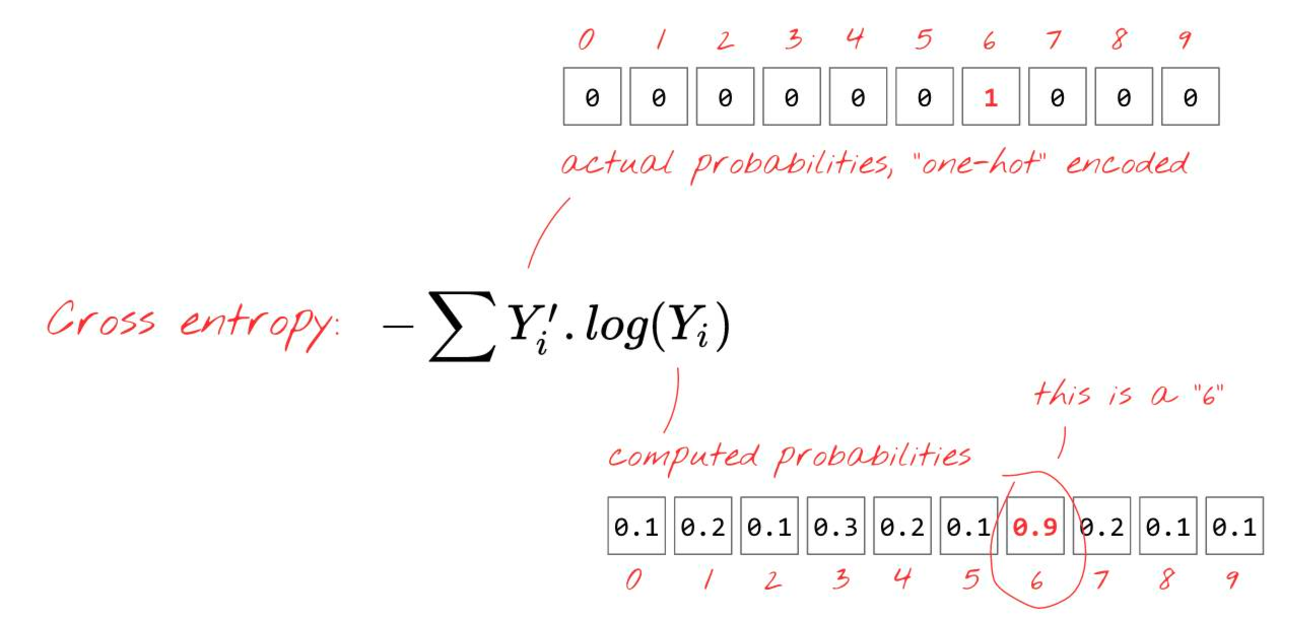
\includegraphics[width=0.8\textwidth]{figures/mnist-cross-entropy.png}
\caption{交叉熵损失函数}
 \label{fig:mnist-cross-entropy}
\end{figure}

\subsubsection{精度}

\code{tf.argmax(y,1)}将按第\ascii{1}个维度计算最大值的索引。既按照${{\text{y}}_{{\text{100}} \times {\text{10}}}}$的每一行,计算得到在每一行中最大值的的索引值。因此,\code{tf.argmax(y,1)}将得到大小为\code{[100, 1]}的矩阵,或大小为\ascii{100}的向量。同样地,\code{tf.argmax(t,1)}也是一个大小为\ascii{100}的向量。

然后,使用\code{tf.equal}将它们逐元素(\ascii{element-wise})进行相等性比较,得到大小为\ascii{100}的布尔向量。为了计算精度,先将布尔向量转别为数值向量,最终求取该数值向量的均值。

\begin{leftbar}
\begin{python}
is_correct = tf.equal(tf.argmax(y,1), tf.argmax(t,1))
accuracy = tf.reduce_mean(tf.cast(is_correct, tf.float32))
\end{python}
\end{leftbar}

\subsection{优化算法}

接下来,使用梯度下降算法实现交叉熵损失函数的最小化。其中,\code{learning\_rate}表示学习速率,描述参数更新的快慢和步伐大小,是一个典型的超参。

\begin{leftbar}
\begin{python}
optimizer = tf.train.GradientDescentOptimizer(learning_rate=0.003)
train_step = optimizer.minimize(cross_entropy)
\end{python}
\end{leftbar}

如\refig{mnist-gd}所示,可以将损失函数比作一座山,登山者试图寻找最佳的行动方案达到山谷。登山者站在某个山坡上环顾四周,决定沿梯度的反方向向下走一小步,直到达到局部最优。

当实施梯度下降更新算法时,初始点不同,获得的最小值也不同,因此梯度下降求得的只是局部最小值。另外,越接近最小值时,下降速度越慢。下降的步伐大小也非常重要,如果太小,则找到函数最小值的速度就很慢;如果太大,则可能会越过极值点。

\begin{figure}[H]
\centering
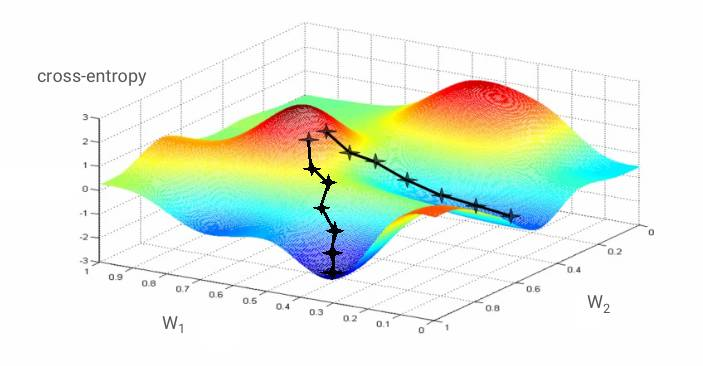
\includegraphics[width=0.8\textwidth]{figures/mnist-gd.jpeg}
\caption{梯度下降算法}
 \label{fig:mnist-gd}
\end{figure}

\subsection{训练模型}

在此之前,\tf{}仅构造计算图,并没有启动计算图的执行。接下来,客户端创建一个会话,建立与本地或远端计算设备集的通道,启动计算图的执行过程。

首先,完成训练参数的初始化。通过运行模型参数的初始化子图,并发地执行各个训练参数的初始化器,将初始值就地修改到相应的训练参数内。

\begin{leftbar}
\begin{python}
with tf.Session() as sess:
  sess.run(init_op)
\end{python}
\end{leftbar}

然后,开始迭代地执行\code{train\_step},完成模型的一次迭代训练。其中,每\ascii{100}次迭代,计算当前模型在训练数据集及测试数据集的精度和损失。

\begin{leftbar}
\begin{python}
with tf.Session() as sess:
  for step in range(1000):
    batch_xs, batch_ys = mnist.train.next_batch(100)        
    sess.run(train_step, feed_dict={x: batch_xs, t: batch_ys})
    
    if step % 100 == 0:
      acc, loss = sess.run([accuracy, cross_entropy], 
        feed_dict={x: batch_xs, t: batch_ys})
      acc, loss = sess.run([accuracy, cross_entropy], 
        feed_dict={x: mnist.test.images, t: mnist.test.labels}) 
\end{python}
\end{leftbar}

据统计,经过\ascii{1000}次迭代,可得到大约\percent{92}的精度。

\begin{figure}[H]
\centering
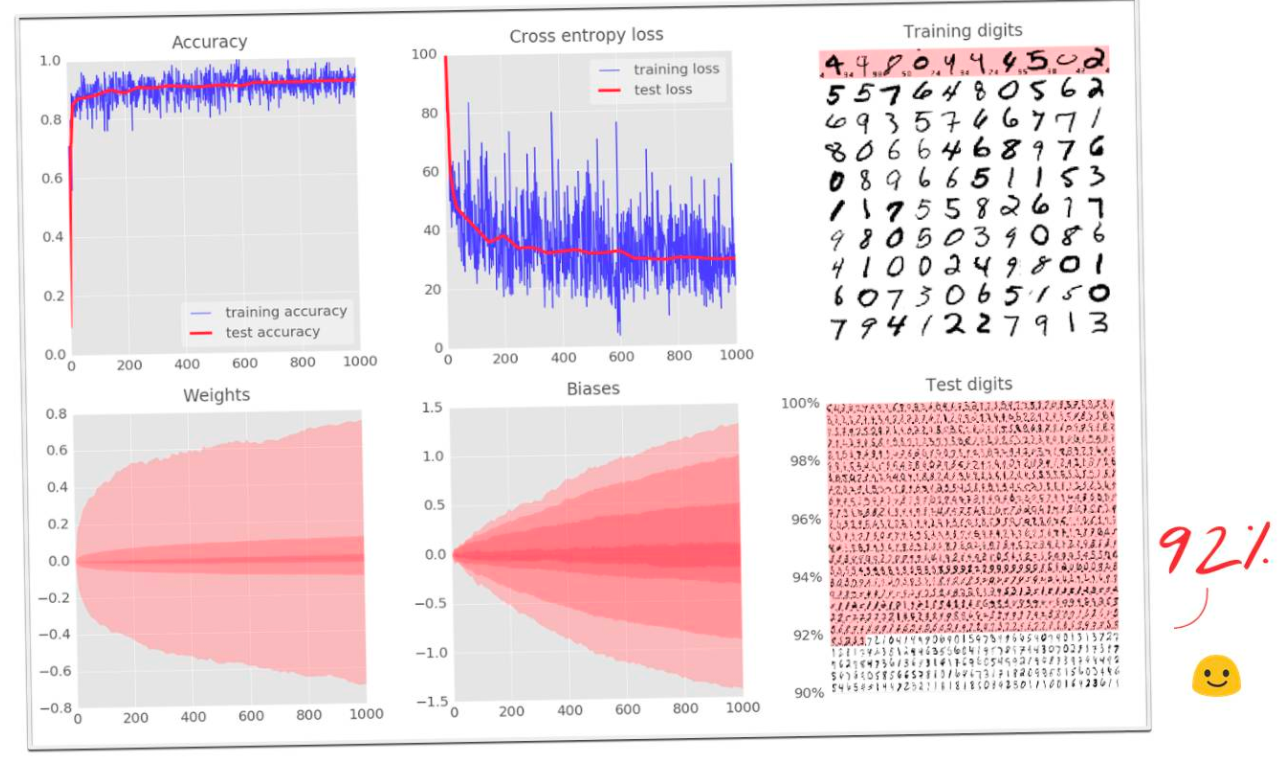
\includegraphics[width=0.8\textwidth]{figures/mnist-slp-accuracy.png}
\caption{可视化:单层感知器,运行1000次step}
 \label{fig:mnist-slp-accuracy}
\end{figure}

\end{content}

\section{多层感知器}

\begin{content}

为了进一步提高精度,接下来尝试搭建\ascii{5}层的多层感知器模型。

\begin{figure}[H]
\centering
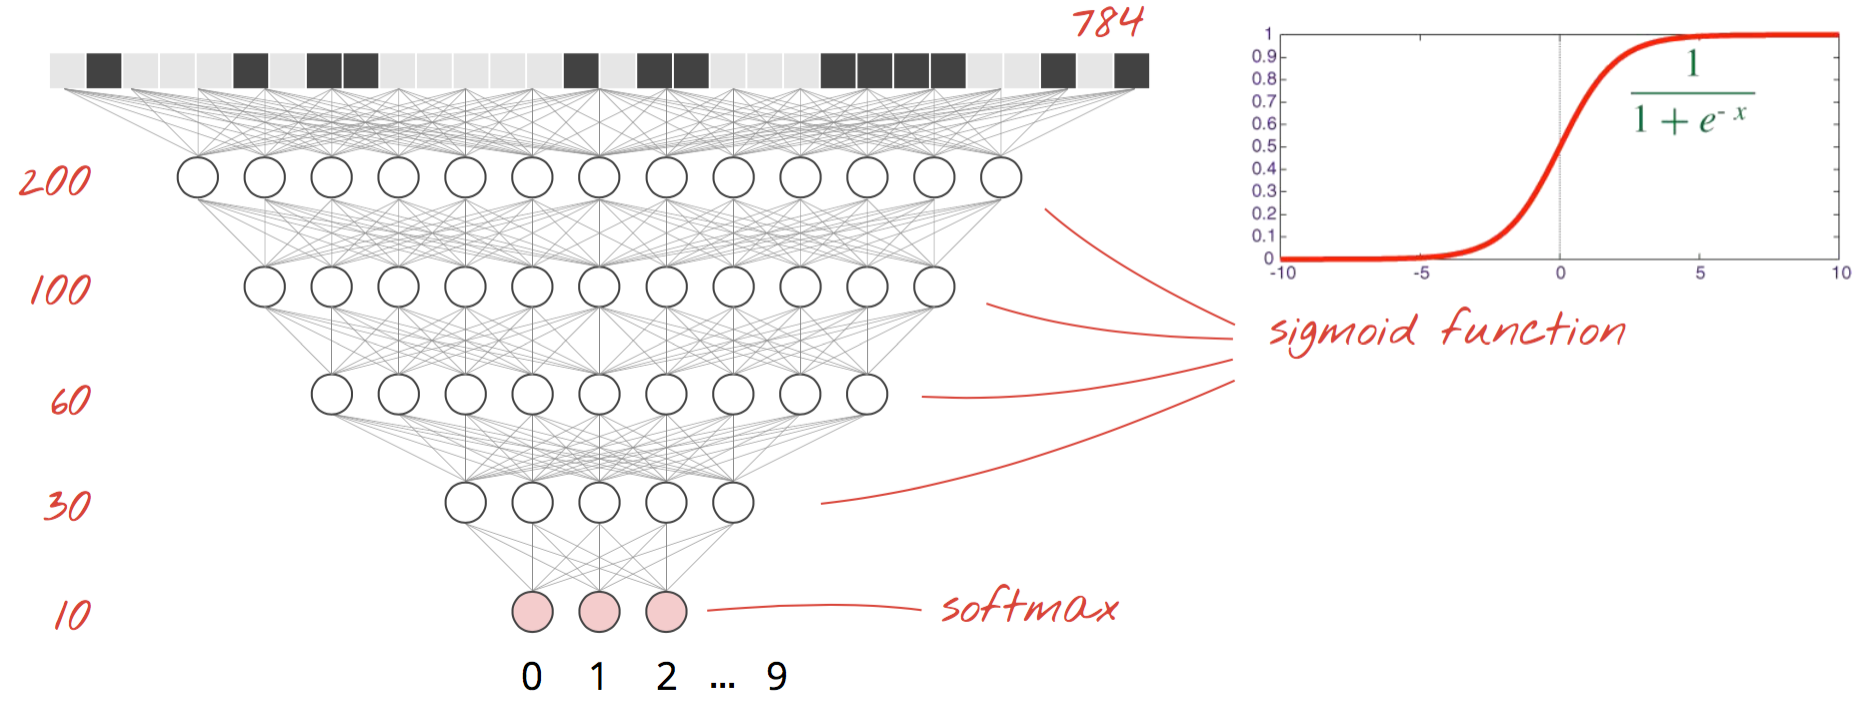
\includegraphics[width=0.8\textwidth]{figures/mnist-5-layer.png}
\caption{5层感知器}
 \label{fig:mnist-5-layer}
\end{figure}

\subsection{理论基础}

\subsubsection{符号定义}

为了形式化地描述多层感知器模型,此处定义了一些常用符号。

\begin{itemize}
   \item \alert{$ {n_{\ell}} $}: 网络层数,其中第$0$层为输入层,第$n_{\ell}$层为输出层
   \item \alert{$ {s_{\ell}} $}: 第$\ell$层的节点数,$ \ell = 0, 1, ..., n_{\ell} $
   \item \alert{$ w_{ji}^{(\ell)} $}: 第$(\ell-1)$层节点$i$与第$\ell$层节点$j$之间的权重,$ \ell = 1, ..., n_{\ell} $
   \item \alert{$ b_i^{(\ell)} $}: 第$\ell$层节点$i$的偏置项,$ \ell = 1, ..., n_{\ell} $
   \item \alert{$ a_i^{(\ell)} $}: 第$\ell$层节点$i$的输出,$ \ell = 1, ..., n_{\ell}, x = a^{(0)}, y = a^{(n_{\ell})} $
   \item \alert{$ z_i^{(\ell)} $}: 第$\ell$层节点$i$的权重和,$ \ell = 1, ..., n_{\ell} $
   \item \alert{$ \delta _i^{(\ell)} $}: 第$\ell$层节点$i$的误差项,$ \ell = 1, ..., n_{\ell} $
   \item \alert{$ S = \{ ({x^{(t)}},{y^{(t)}});t = 1,2,...,m\} $}: 样本空间
 \end{itemize}

\subsubsection{前向传播}

$z^{(\ell )}$表示$\ell$层的线性加权和,它由第$\ell - 1$层的输出$a^{(\ell  - 1)}$与第$\ell$层的权重矩阵$w^{(\ell )}$相乘,再加上第$\ell$层的偏置向量所得。

推而广之,第$\ell$层的输出,由激活函数$f({z^{(\ell )}})$所得。其中,$a^{(0)}} = x, y = {a^{({n_\ell })}}$。

\[\begin{gathered}
  {z^{(\ell )}} = {w^{(\ell )}}{a^{(\ell  - 1)}} + {b^{(\ell )}} \hfill \\
  {a^{(\ell )}} = f({z^{(\ell )}}) \hfill \\
  {a^{(0)}} = x \hfill \\
  y = {a^{({n_\ell })}} \hfill \\ 
\end{gathered} \]

\subsubsection{后向传播}

然后,反向计算各层的误差。其中,第$\ell$层的误差,由$\ell + 1$层的误差计算所得。特殊地,在输出层,预测值$a^{({n_\ell })}$与$y$之间的误差,可以直接计算得到。

\[{\delta ^{(\ell)}} = \left\{ \begin{gathered}
  {({w^{(\ell + 1)}})^T}{\delta ^{(\ell + 1)}} \circ f\,'({z^{(\ell)}});{\text{  }}\ell \ne {n_\ell} \hfill \\
  ({a^{(\ell)}} - y) \circ f\,'({z^{(\ell)}}); {\text{  }}\ell = {n_\ell} \hfill \\ 
\end{gathered}  \right.\]

损失函数$J(w,b)$相对于各层的权重矩阵与偏置向量的梯度便可以计算得到。

\[\begin{gathered}
  {\nabla _{{w^{(\ell )}}}}J(w,b;x,y) = {\delta ^{(\ell )}}{\left( {{a^{(\ell  - 1)}}} \right)^T} \hfill \\
  {\nabla _{{b^{(\ell )}}}}J(w,b;x,y) = {\delta ^{(\ell )}} \hfill \\
  \ell  = 1,2,...,{n_\ell } \hfill \\ 
\end{gathered} \]

一般地,在实际系统实现中,下游层传递梯度给上层,上层直接完成梯度的计算。

\subsubsection{参数更新}

对于给定样本数据集$ S = \{ ({x^{(t)}},{y^{(t)}});t = 1,2,...,m\} $,根据梯度反传公式,可以计算得到参数更新的变化量。

\[\begin{aligned}
  \Delta {w^{(\ell )}} \leftarrow \Delta {w^{(\ell )}} + {\nabla _{{w^{(\ell )}}}}J\left( {w,b;{x^{(t)}},{y^{(t)}}} \right) \\ 
  \Delta {b^{(\ell )}} \leftarrow \Delta {b^{(\ell )}} + {\nabla _{{b^{(\ell )}}}}J\left( {w,b;{x^{(t)}},{y^{(t)}}} \right) \\ 
  t = 1,2,...,m;\ell  = 1,2,...,{n_\ell } \\ 
\end{aligned} \]

最后,执行梯度下降算法,完成训练参数一个迭代的更新。

\[\begin{aligned}
  {w^{(\ell )}} \leftarrow  & {w^{(\ell )}} - \alpha \left( {\frac{{\Delta {w^{(\ell )}}}}{m}} \right) \\ 
  {b^{(\ell )}} \leftarrow  & {b^{(\ell )}} - \alpha \frac{{\Delta {b^{(\ell )}}}}{m} \\ 
  \ell  = & 1,2,...,{n_\ell }  \\
\end{aligned} \]

\subsection{定义模型}

相对于上一节中尝试的单层感知器,此处定义每一个隐式层的权重时,并没有使用常量定义变量的初始值,而使用满足某种数据分布特征的随机值。

\begin{leftbar}
\begin{python}
K = 200
L = 100
M = 60
N = 30

w1 = tf.Variable(tf.truncated_normal([28*28, K] ,stddev=0.1)) 
b1 = tf.Variable(tf.zeros([K]))

w2 = tf.Variable(tf.truncated_normal([K, L], stddev=0.1))
b2 = tf.Variable(tf.zeros([L]))

w3 = tf.Variable(tf.truncated_normal([L, M], stddev=0.1)) 
b3 = tf.Variable(tf.zeros([M]))

w4 = tf.Variable(tf.truncated_normal([M, N], stddev=0.1)) 
b4 = tf.Variable(tf.zeros([N]))

w5 = tf.Variable(tf.truncated_normal([N, 10], stddev=0.1)) 
b5 = tf.Variable(tf.zeros([10]))
\end{python}
\end{leftbar}

在定义每一个隐式层时,采用\ascii{sigmoid}的激活函数。而在最后的输出层,采用\ascii{softmax}的激活函数。

\begin{leftbar}
\begin{python}
y1 = tf.nn.sigmoid(tf.matmul(x,  w1) + b1)
y2 = tf.nn.sigmoid(tf.matmul(y1, w2) + b2)
y3 = tf.nn.sigmoid(tf.matmul(y2, w3) + b3)
y4 = tf.nn.sigmoid(tf.matmul(y3, w4) + b4)
y  = tf.nn.softmax(tf.matmul(y4, w5) + b5)
\end{python}
\end{leftbar}

经过迭代的模型训练,可以得到大约\percent{97}左右的精度。但是,网络随着层次的增加,模型变得越来越难以收敛。接下来,尝试一些常见的调优技术,改善网络的性能。

\subsection{优化技术}

\subsubsection{激活函数:ReLU}

在深度模型中,不适合使用\ascii{sigmoid}激活函数。它将把所有的值都挤到了\ascii{0}到\ascii{1}之间;随着网络层次的增加,引发梯度消失的问题。

\begin{figure}[H]
\centering
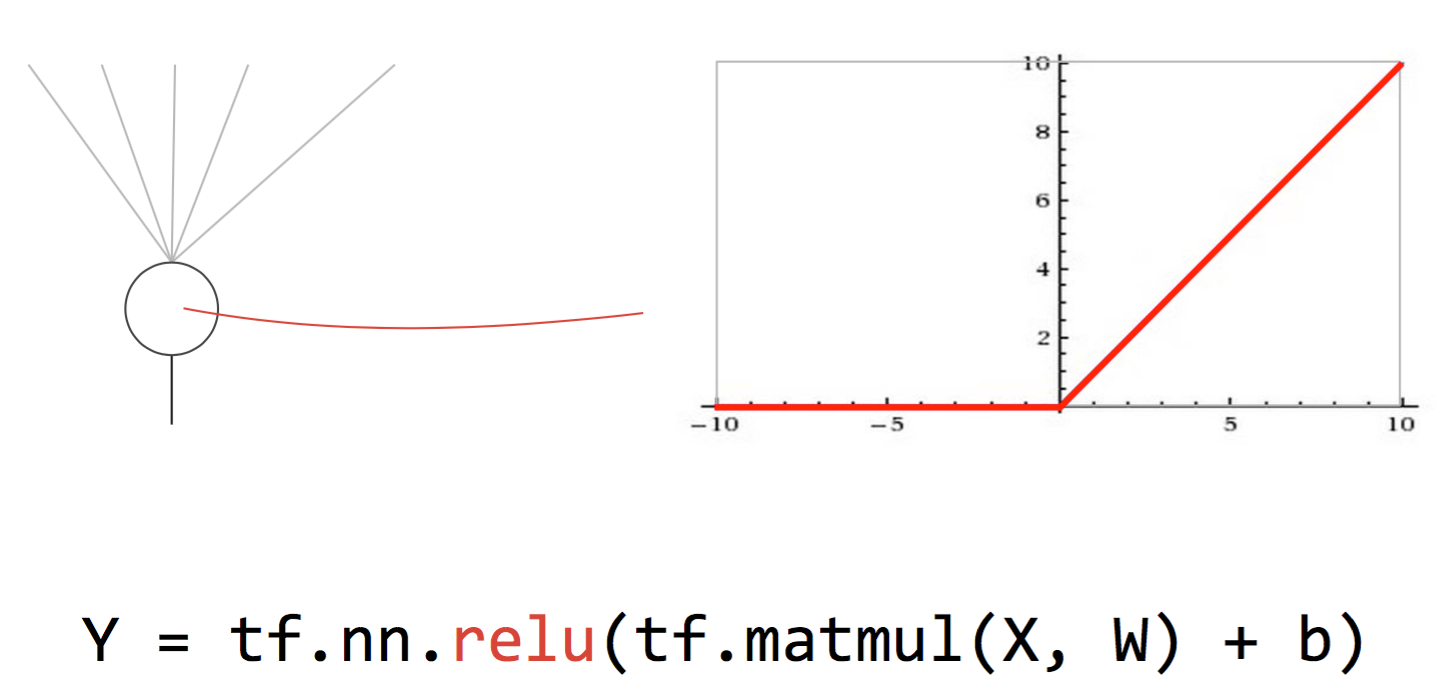
\includegraphics[width=0.8\textwidth]{figures/mnist-relu.png}
\caption{ReLU激活函数}
 \label{fig:mnist-relu}
\end{figure}

可以使用\ascii{ReLU(Rectified Linear Unit)}替代\ascii{sigmoid},不仅避免了\ascii{sigmoid}导致的一些问题,而且能够加快初始的收敛速度。

\begin{leftbar}
\begin{python}
y1 = tf.nn.relu(tf.matmul(x,  w1) + b1)
y2 = tf.nn.relu(tf.matmul(y1, w2) + b2)
y3 = tf.nn.relu(tf.matmul(y2, w3) + b3)
y4 = tf.nn.relu(tf.matmul(y3, w4) + b4)
y  = tf.nn.softmax(tf.matmul(y4, w5) + b5)
\end{python}
\end{leftbar}

另外,如果使用\ascii{ReLU}激活函数,偏置向量常常初始化为小的正值,使得神经元在一开始就会工作在\ascii{ReLU}的非零区域内。

\begin{leftbar}
\begin{python}
K = 200
L = 100
M = 60
N = 30

w1 = tf.Variable(tf.truncated_normal([28*28, K] ,stddev=0.1)) 
b1 = tf.Variable(tf.ones([L])/10)

w2 = tf.Variable(tf.truncated_normal([K, L], stddev=0.1))
b2 = tf.Variable(tf.ones([L])/10)

w3 = tf.Variable(tf.truncated_normal([L, M], stddev=0.1)) 
b3 = tf.Variable(tf.ones([L])/10)

w4 = tf.Variable(tf.truncated_normal([M, N], stddev=0.1)) 
b4 = tf.Variable(tf.ones([L])/10)

w5 = tf.Variable(tf.truncated_normal([N, 10], stddev=0.1)) 
b5 = tf.Variable(tf.ones([L])/10)
\end{python}
\end{leftbar}

如\refig{mnist-sigmoid-to-relu}所示,前\ascii{300}次迭代,使用\ascii{ReLU}相对于使用\ascii{sigmoid},其初始收敛速度提升显著。

\begin{figure}[H]
\centering
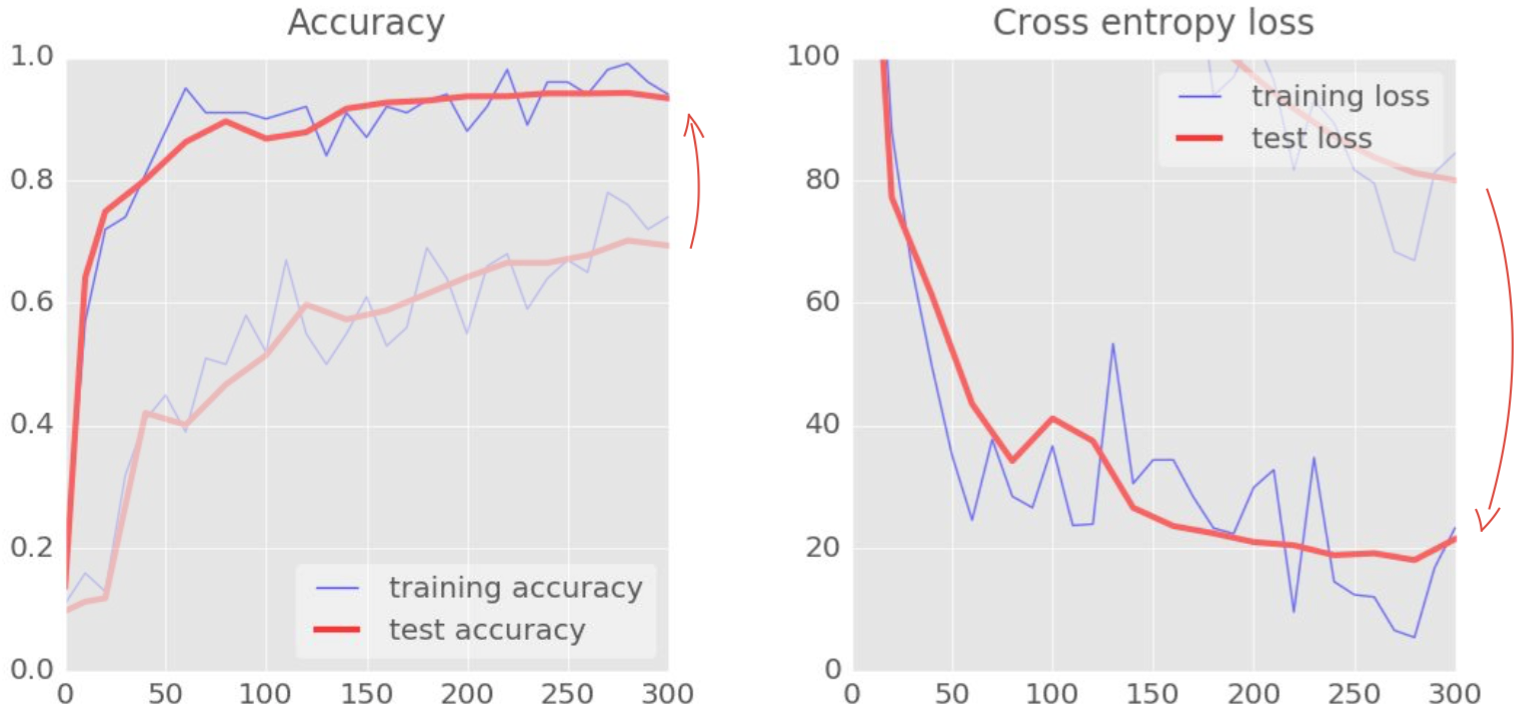
\includegraphics[width=0.8\textwidth]{figures/mnist-sigmoid-to-relu.png}
\caption{应用ReLU激活函数:初始收敛速度提升显著}
 \label{fig:mnist-sigmoid-to-relu}
\end{figure}

\subsubsection{不定值}

为了得到稳定的数值计算结果,避免出现精度突降为\ascii{0}的情况发生。追溯实现代码,可能引入\code{log(0)}计算得到\code{NaN}不定值的问题。可以使用\code{softmax\_cross\_entropy\_with\_logits}计算交叉熵损失,并将线性加权和作为其输入(常称为\ascii{logits})。

\begin{leftbar}
\begin{python}
logits = tf.matmul(y4, w5) + b5
y = tf.nn.softmax(logits)

cross_entropy = tf.nn.softmax_cross_entropy_with_logits(
  logits=logits, labels=t)
\end{python}
\end{leftbar}

\subsubsection{学习速率衰减}

随着网路层次的增加,及其应用相关优化技术后,模型的精度能够能得到\percent{98}左右,但很难得到一个稳定的精度。如\refig{mnist-lr-too-larger}所示,精度和损失抖动相当明显。

\begin{figure}[H]
\centering
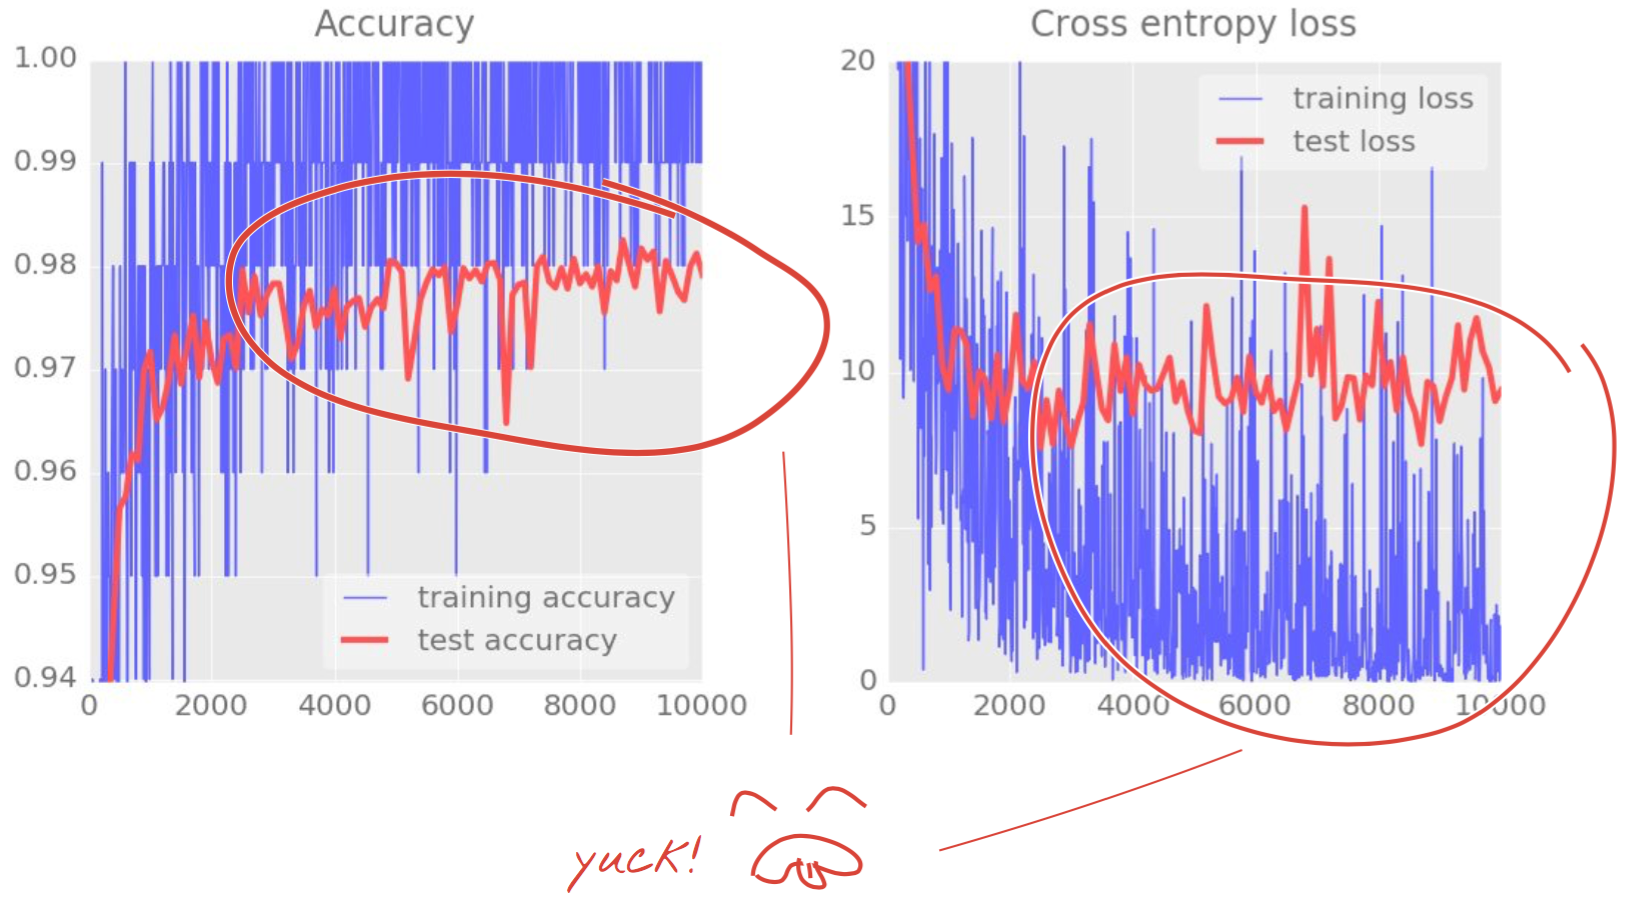
\includegraphics[width=0.8\textwidth]{figures/mnist-lr-too-larger.png}
\caption{噪声抖动:学习速率过大}
 \label{fig:mnist-lr-too-larger}
\end{figure}

可以采用更好的优化算法,例如\code{AdamOptimizer}。随着迭代过程的次数,学习速率将指数级衰减,在模型训练后期可以得到一个更稳定的精度和损失曲线。

\begin{leftbar}
\begin{python}
lr = tf.placeholder(tf.float32)
train_step = tf.train.AdamOptimizer(lr).minimize(cross_entropy)
\end{python}
\end{leftbar}

在每个迭代训练过程中,根据当前\code{step}的值,实时计算当前迭代的学习速率\code{lr},然后通过\code{feed\_dict}传递给\code{Session.run}执行。其中,学习速率衰减方程如下代码所示,随着迭代次数的增加,学习速率指数衰减。

\begin{leftbar}
\begin{python}
def lr(step):
  max_lr, min_lr, decay_speed = 0.003, 0.0001, 2000.0
  return min_lr + (max_lr - min_lr) * math.exp(-step/decay_speed)

with tf.Session() as sess:
  for step in range(10000):
    batch_xs, batch_ys = mnist.train.next_batch(100)
    sess.run(train_step, 
      feed_dict={x: batch_xs, t: batch_ys, pkeep: 0.75, lr: lr(step)})
\end{python}
\end{leftbar}

如\refig{mnist-apply-learning-rate-decay}所示,应用学习速率衰减方法后,可以得到一个更稳定的精度和损失曲线。

\begin{figure}[H]
\centering
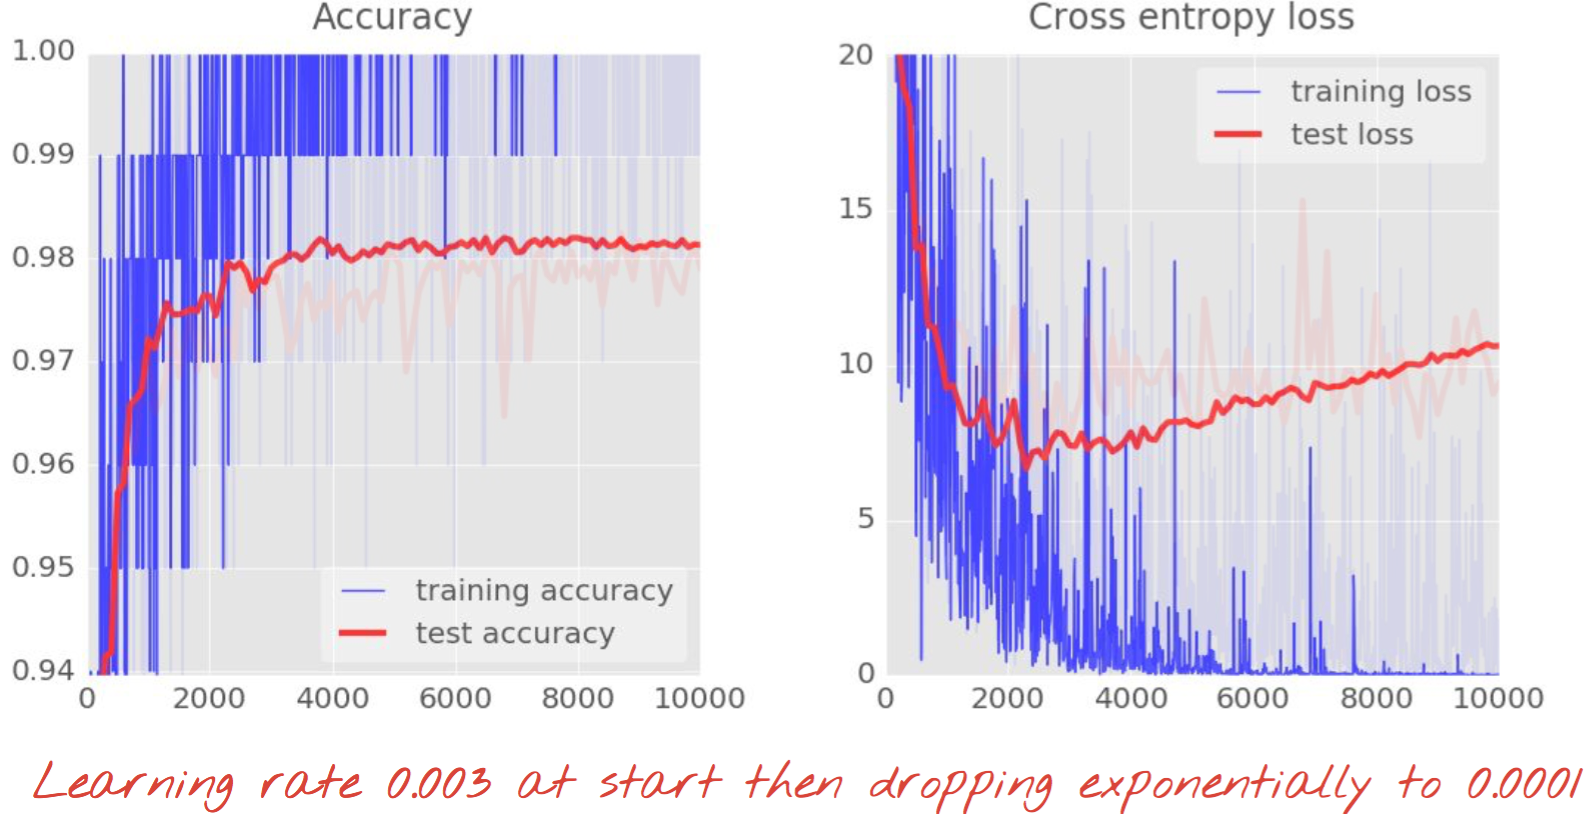
\includegraphics[width=0.8\textwidth]{figures/mnist-apply-learning-rate-decay.png}
\caption{应用Adam优化算法后,精度和损失趋于稳定}
 \label{fig:mnist-apply-learning-rate-decay}
\end{figure}

\subsubsection{应用Dropout}

但是,损失曲线在训练集与测试集上相分离,出现明显的过拟合现象。即模型在训练数据集上表现良好,但在测试数据集上出现反弹,模型缺乏足够的泛化能力。

\begin{figure}[H]
\centering
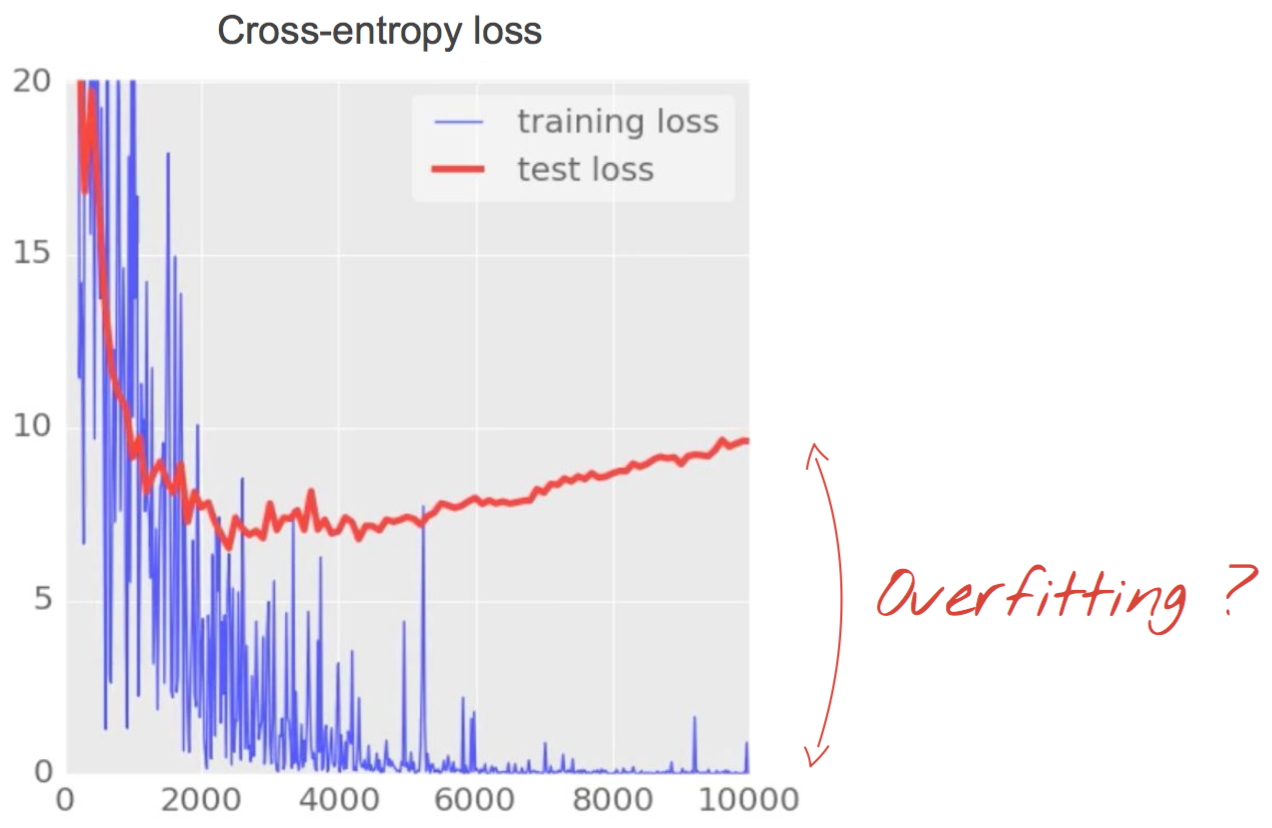
\includegraphics[width=0.8\textwidth]{figures/mnist-overfitting.png}
\caption{过拟合}
 \label{fig:mnist-overfitting}
\end{figure}

如\refig{mnist-dropout}所示,在训练时对隐藏层的输出实施\ascii{dropout}操作,以\code{1 - pkeep}的概率随机丢弃神经元的输出,并在反向传播梯度时不再更新相应的权重。而在推理时恢复所有神经元的输出,间接改善了网络的泛化能力。

\begin{figure}[H]
\centering
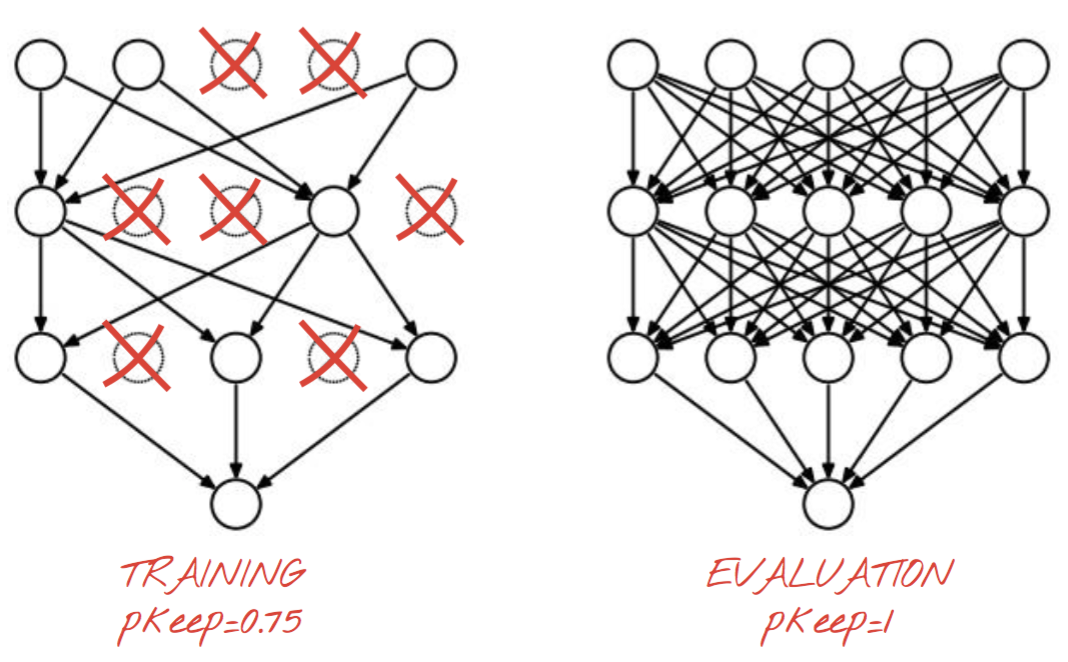
\includegraphics[width=0.8\textwidth]{figures/mnist-dropout.png}
\caption{Dropout方法}
 \label{fig:mnist-dropout}
\end{figure}

使用\tf{}实现\ascii{dropout}操作时,先定义一个超级参数\code{pkeep},表示隐藏层的神经元以概率\code{pkeep}随机保留,以概率\code{1 - pkeep}随机丢弃。

\begin{leftbar}
\begin{python}
pkeep = tf.placeholder(tf.float32)

y1 = tf.nn.relu(tf.matmul(x,  w1) + b1)
y1d = tf.nn.dropout(y1, pkeep)

y2 = tf.nn.relu(tf.matmul(y1d, w2) + b2)
y2d = tf.nn.dropout(y2, pkeep)

y3 = tf.nn.relu(tf.matmul(y2d, w3) + b3)
y3d = tf.nn.dropout(y3, pkeep)

y4 = tf.nn.relu(tf.matmul(y3d, w4) + b4)
y4d = tf.nn.dropout(y4, pkeep)

logits = tf.matmul(y4d, w5) + b5
y = tf.nn.softmax(Ylogits)
\end{python}
\end{leftbar}

在训练时,置超参\code{pkeep}的值小于\ascii{1};而在推理时,置超参\code{pkeep}的值为\ascii{1}。

\begin{leftbar}
\begin{python}
with tf.Session() as sess:
  for step in range(10000):
    batch_xs, batch_ys = mnist.train.next_batch(100)
    sess.run(train_step, 
      feed_dict={x: batch_xs, t: batch_ys, pkeep: 0.75, lr: lr(step)})

    if step % 100 == 0:
      acc, loss = sess.run([accuracy, cross_entropy], 
        feed_dict={x: batch_xs, t: batch_ys, pkeep: 1})
      acc, loss = sess.run([accuracy, cross_entropy], 
        feed_dict={x: mnist.test.images, t: mnist.test.labels, pkeep: 1})
\end{python}
\end{leftbar}

在每一隐藏层实施\ascii{dropout}操作之后,训练集与测试集的损失曲线再次相交。但是,精度和损失曲线相比又出现小幅的抖动,而且训练集与测试集的损失曲线相重合的程度不是很理想,过拟合问题依然很突出。

也就是说,过拟合问题存在其他更深刻的原因。例如,将$ 28 \times 28 $的图片实施扁平化操作,将其变换为一个长度为\ascii{784}的一维向量,这将完全丢失了像素的空间排列信息。

接下来,通过尝试构造卷积神经网络,从原图像中提取特征,从而保留了像素的空间排列信息,进而提升网络的性能。

\begin{figure}[H]
\centering
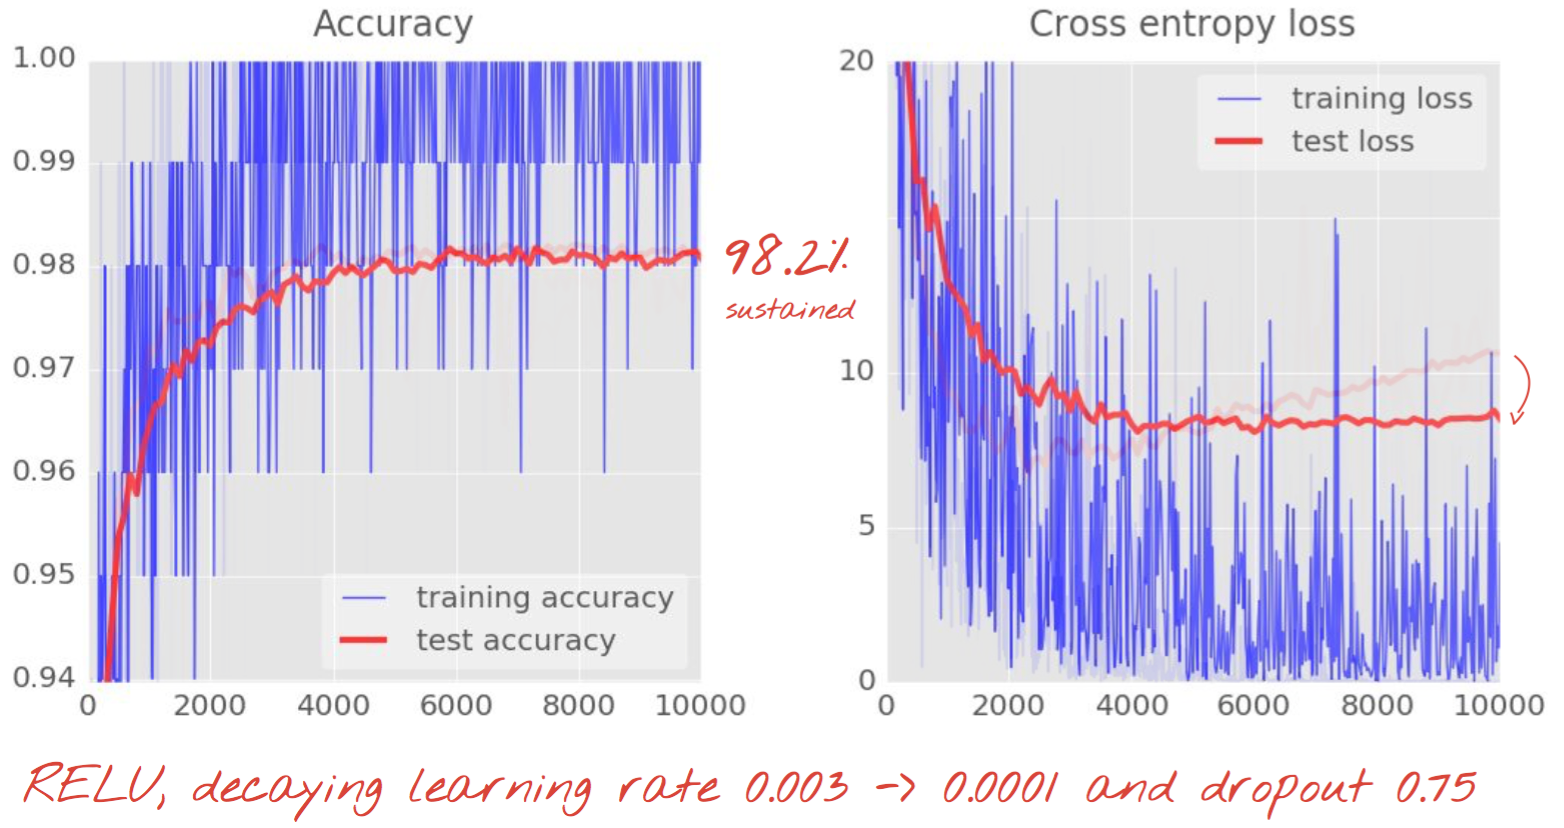
\includegraphics[width=0.8\textwidth]{figures/mnist-apply-dropout-result.png}
\caption{实施Dropout后,训练集与测试集的损失曲线再次重合}
 \label{fig:mnist-apply-dropout-result}
\end{figure}

\end{content}

\section{卷积网络}

\begin{content}

\subsection{特征与优势}

随着网络层次增加,全连接网络的梯度消失的问题将越发突出,收敛速度变得越来越慢。相对于全连接网络,卷积网络具有\ascii{3}个主要特征,它减少了网络参数的数量,提升网络的泛化能力。

\subsubsection{局部连接}

相对于全连接网络,卷积网络实现了局部连接,即每个神经元并不与上一层的神经元都存在连接。如\refig{mnist-conv-local-conn}左侧所示,假如存在一张$ 1000 \times 1000 $像素的图像,及其$ 10^6 $个隐藏层的神经元。在全连接网络里,将拥有$ 10^3 \times 10^3 \times 10^6 = 10^12 $个训练参数。

事实上,每个神经元没有必要与上一层神经元都存在连接。如\refig{mnist-conv-local-conn}右侧所示,假如每个隐藏层的神经元仅与上一层$ 10 \times 10 $的局部图像存在连接,$ 10^6 $个隐藏层的神经元则需要$ 10^6 \times 10^2 = 10^8$个网络连接,相比减少了\ascii{4}个数量级。

\begin{figure}[H]
\centering
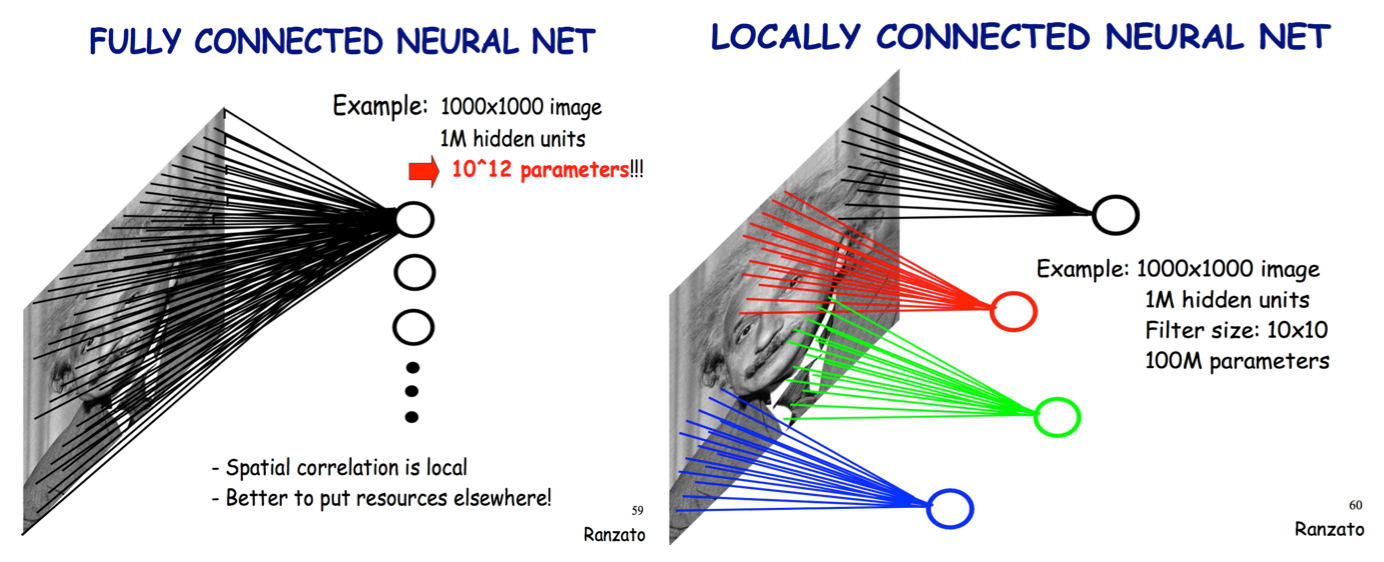
\includegraphics[width=0.9\textwidth]{figures/mnist-conv-local-conn.png}
\caption{局部连接}
 \label{fig:mnist-conv-local-conn}
\end{figure}

\subsubsection{权值共享}

为了进一步减少网络连接,卷积网络还实现了权重共享;即每一组连接共享相同的权重,而不是每个连接存在不同的权重。如\refig{mnist-conv-local-conn-2}右侧所示,每个隐藏层的神经元仅与$ 10 \times 10 $的局部图像存在连接,且共享$ 10 \times 10 $的权重矩阵,与隐藏层的神经元的数目无关。相对于如\refig{mnist-conv-local-conn-2}左侧的局部连接网络,需要$10^8$个参数,卷积层仅需$10^2$个参数。

如\refig{mnist-conv-local-conn-2}右侧所示,为了提取不同特征,例如不同边缘的图像特征,可以使用多个过滤器。例如,存在\ascii{100}个过滤器,则需要$10^4$个参数。

\begin{figure}[H]
\centering
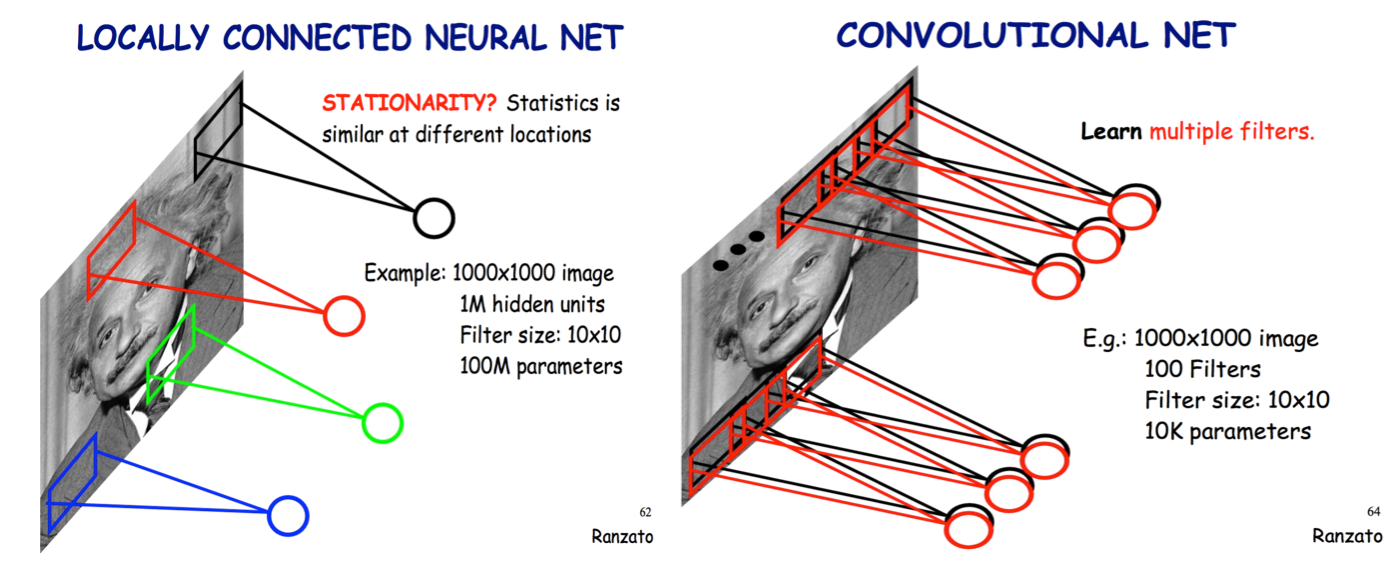
\includegraphics[width=0.9\textwidth]{figures/mnist-conv-local-conn-2.png}
\caption{权值共享,多个过滤器}
 \label{fig:mnist-conv-local-conn-2}
\end{figure}

\subsubsection{下采样}

如\refig{mnist-subsample}所示,可选地实施下采样,进一步减少网络的参数,提升模型的鲁棒性。

\begin{figure}[H]
\centering
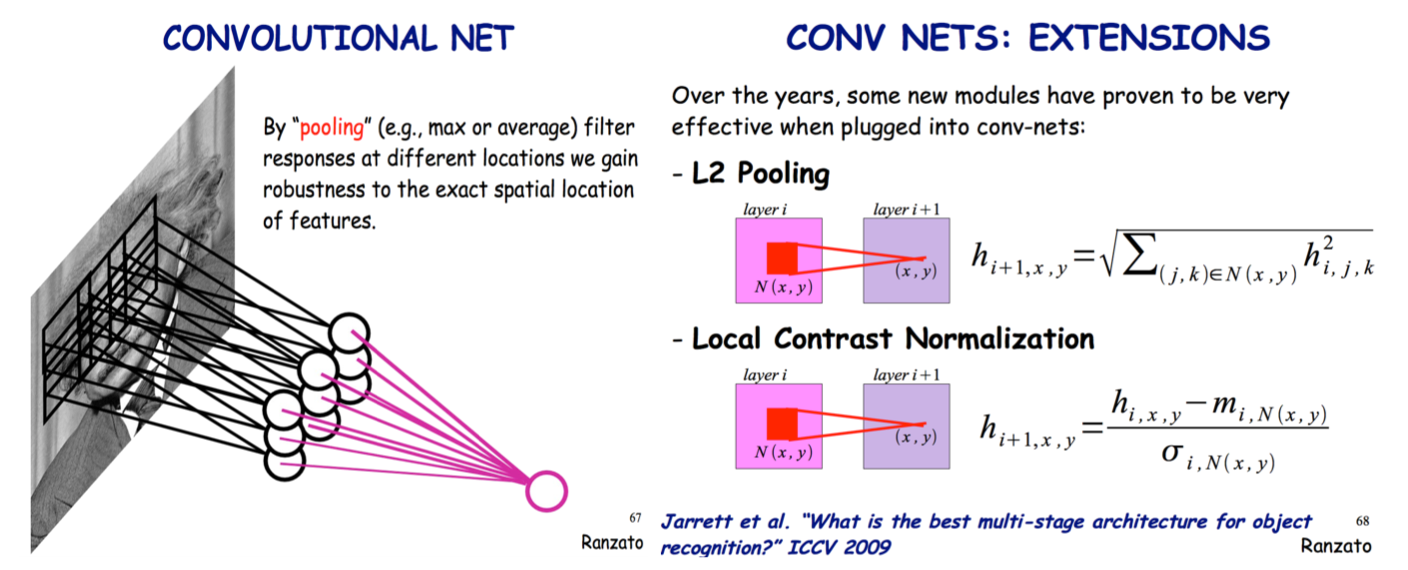
\includegraphics[width=0.9\textwidth]{figures/mnist-subsample.png}
\caption{下采样}
 \label{fig:mnist-subsample}
\end{figure}

\subsection{卷积运算}

卷积运算是一个计算密集型的\ascii{OP}。如\refig{mnist-conv2d-gif}所示,存在一个权重向量\code{w[3,3,3,2]},其中输入通道数为\ascii{3},输出通道数为\ascii{2},卷积核大小为$3 \times 3$。

显而易见,输入图像的通道数,等价于卷积核的深度;卷积核的数目,等于\ascii{Feature Map}的输出通道数。

另外,为了采集图像的边缘特征,在原图像外围补了(\ascii{padding})一圈零值。每次卷积计算,移动的步长(\ascii{stride})为\ascii{2}。因此,最终输出的\ascii{Feature Map}大小为$3 \times 3$。

\begin{figure}[H]
\centering
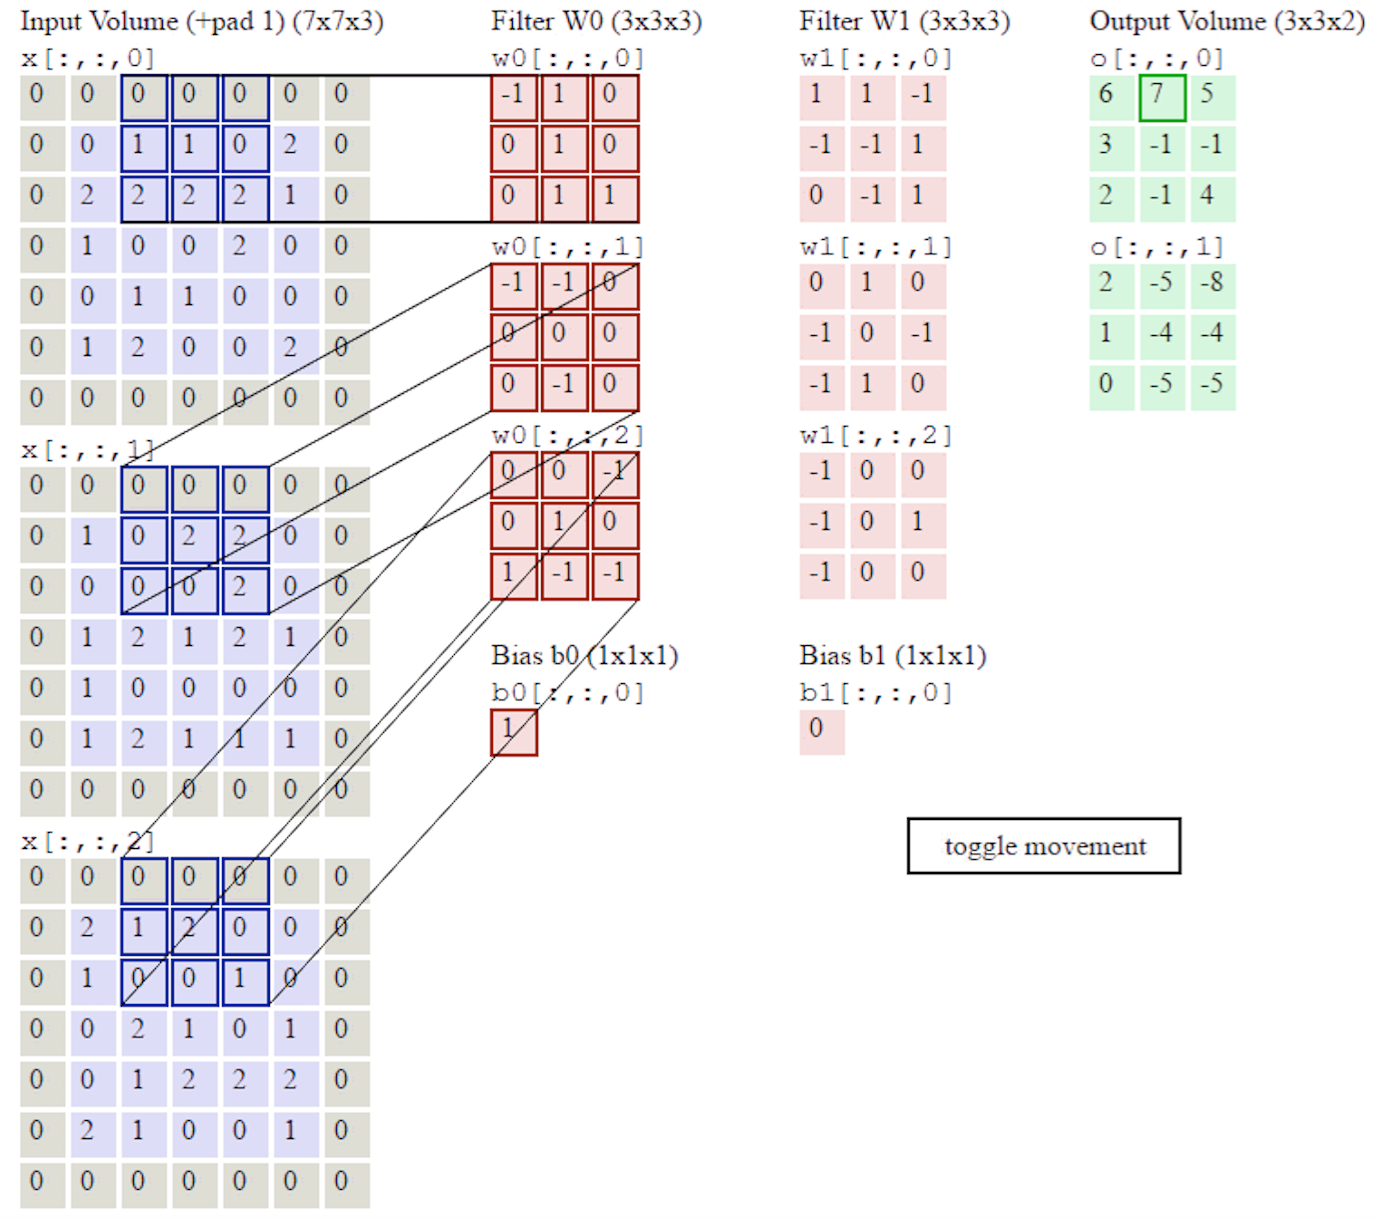
\includegraphics[width=0.8\textwidth]{figures/mnist-conv2d-gif.png}
\caption{卷积运算}
 \label{fig:mnist-conv2d-gif}
\end{figure}

\subsubsection{例子}

加入存在一个$32 \times 32 \times 3$的图片,卷积核大小为$5 \times 5 \times 3$。其中,卷积核的深度等于图片的输入通道数。

如\refig{mnist-conv-1dot}所示,卷积核与图片中其中大小为$5 \times 5 \times 3$的块实施点积运算,得到一个值。

\begin{figure}[H]
\centering
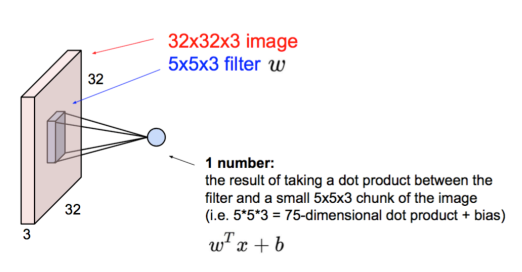
\includegraphics[width=0.8\textwidth]{figures/convolutional-layer-2.png}
\caption{卷积运算:卷积核与图片块的点积运算}
 \label{fig:mnist-conv-1dot}
\end{figure}

如\refig{mnist-conv-ndot}所示,卷积核遍历整个图片空间,最终得到一个大小为$28 \times 28 \times 1$的\ascii{Feature Map}。

\begin{figure}[H]
\centering
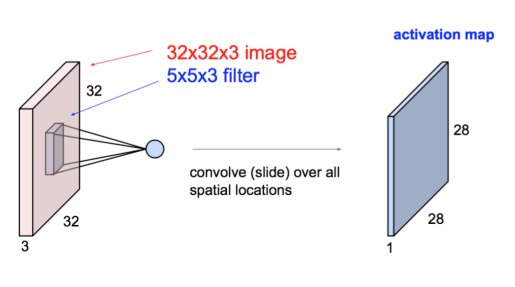
\includegraphics[width=0.8\textwidth]{figures/convolutional-layer-3.png}
\caption{卷积运算:卷积核遍历图片,步长为1}
 \label{fig:mnist-conv-ndot}
\end{figure}

如\refig{mnist-conv-multi-filters}所示,如果存在多个卷积核,则得到多个\ascii{Feature Map}。

\begin{figure}[H]
\centering
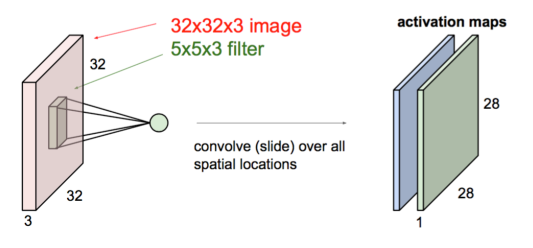
\includegraphics[width=0.8\textwidth]{figures/convolutional-layer-4.png}
\caption{卷积运算:多个卷积核}
 \label{fig:mnist-conv-multi-filters}
\end{figure}

\subsection{公式推导}

\subsubsection{前向传播}

$Z^{(\ell )}$表示$\ell$层的线性加权和,它由第$\ell - 1$层的输出$A^{(\ell  - 1)}$与第$\ell$层的权重矩阵$W^{(\ell )}$卷积,再加上第$\ell$层的偏置向量所得。

推而广之,第$\ell$层的输出,由激活函数$f({Z^{(\ell )}})$所得。其中,$A^{(0)}} = x, y = {A^{({n_\ell })}}$。

\[\begin{gathered}
  {Z^{(\ell )}} = {A^{(\ell  - 1)}} * {W^{(\ell )}} + {b^{(\ell )}} \hfill \\
  {A^{(\ell )}} = f\left( {{Z^{(\ell )}}} \right) \hfill \\ 
\end{gathered} \]

\subsubsection{后向传播}

然后,反向计算各层的误差。其中,第$\ell$层的误差,由$\ell + 1$层的误差计算所得。相对于全连接网络,此处运用的是卷积运算,并非矩阵乘法运算。

\[
{\delta ^{(\ell )}} = {\delta ^{(\ell  + 1)}} * {W^{(\ell  + 1)}} \circ f\,'\left( {{z^{(\ell )}}} \right)
\]

损失函数$J(w,b)$相对于各层的权重矩阵与偏置向量的梯度便可以计算得到。

\[\begin{aligned}
  {\nabla _{{W^{(\ell )}}}}J(W,b) =  & {A^{(\ell  - 1)}} * {\delta ^{(\ell )}} \\ 
  {\nabla _{{b^{(\ell )}}}}J(W,b) =  & {\delta ^{(\ell )}} \\ 
\end{aligned} \]

\subsection{实现卷积网络}

实现卷积网络时,首先需要定义每层过滤器的权重矩阵,用于提取图像的特征。权重矩阵在图像里表现的像一个从原始图像矩阵中提取特定信息的过滤器。一个权重矩阵可能用来提取图像边缘信息,一个权重矩阵可能是用来提取一个特定颜色,另一个权重矩阵可能对不需要的噪声进行模糊化。

当存在多个卷积层时,初始层往往提取较多的一般特征;随着网络结构变得更深,权值矩阵提取的特征越来越复杂,并且越来越适用于眼前的具体问题。

一般地,过滤器常使用一个\ascii{4}维的张量表示,前两维表示过滤器的大小,第三维表示输入的通道数,第四维表示输出的通道数。如\refig{mnist-filter}所示。

\begin{figure}[H]
\centering
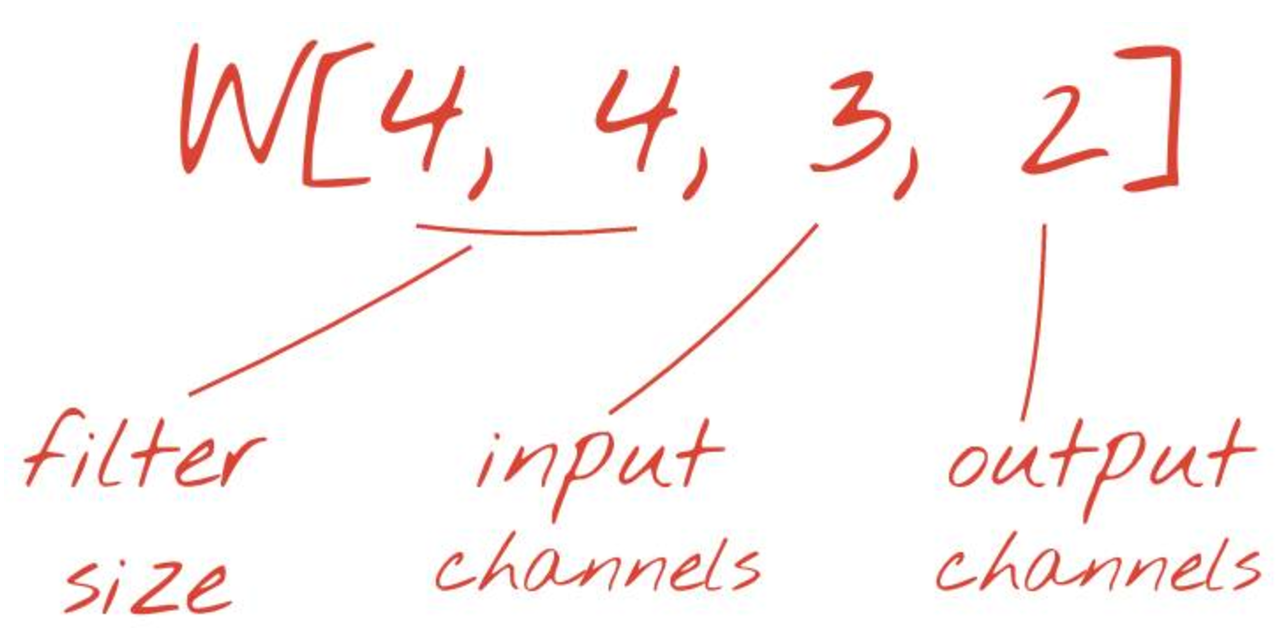
\includegraphics[width=0.4\textwidth]{figures/mnist-filter.png}
\caption{卷积层的过滤器}
 \label{fig:mnist-filter}
\end{figure}

如\refig{mnist-conv2d-1}所示,构造了\ascii{3}个卷积层和\ascii{2}个全连接层。其中,中间隐藏层使用\ascii{ReLU}的激活函数,最后的输出层采用\ascii{softmax}的激活函数。

\begin{figure}[H]
\centering
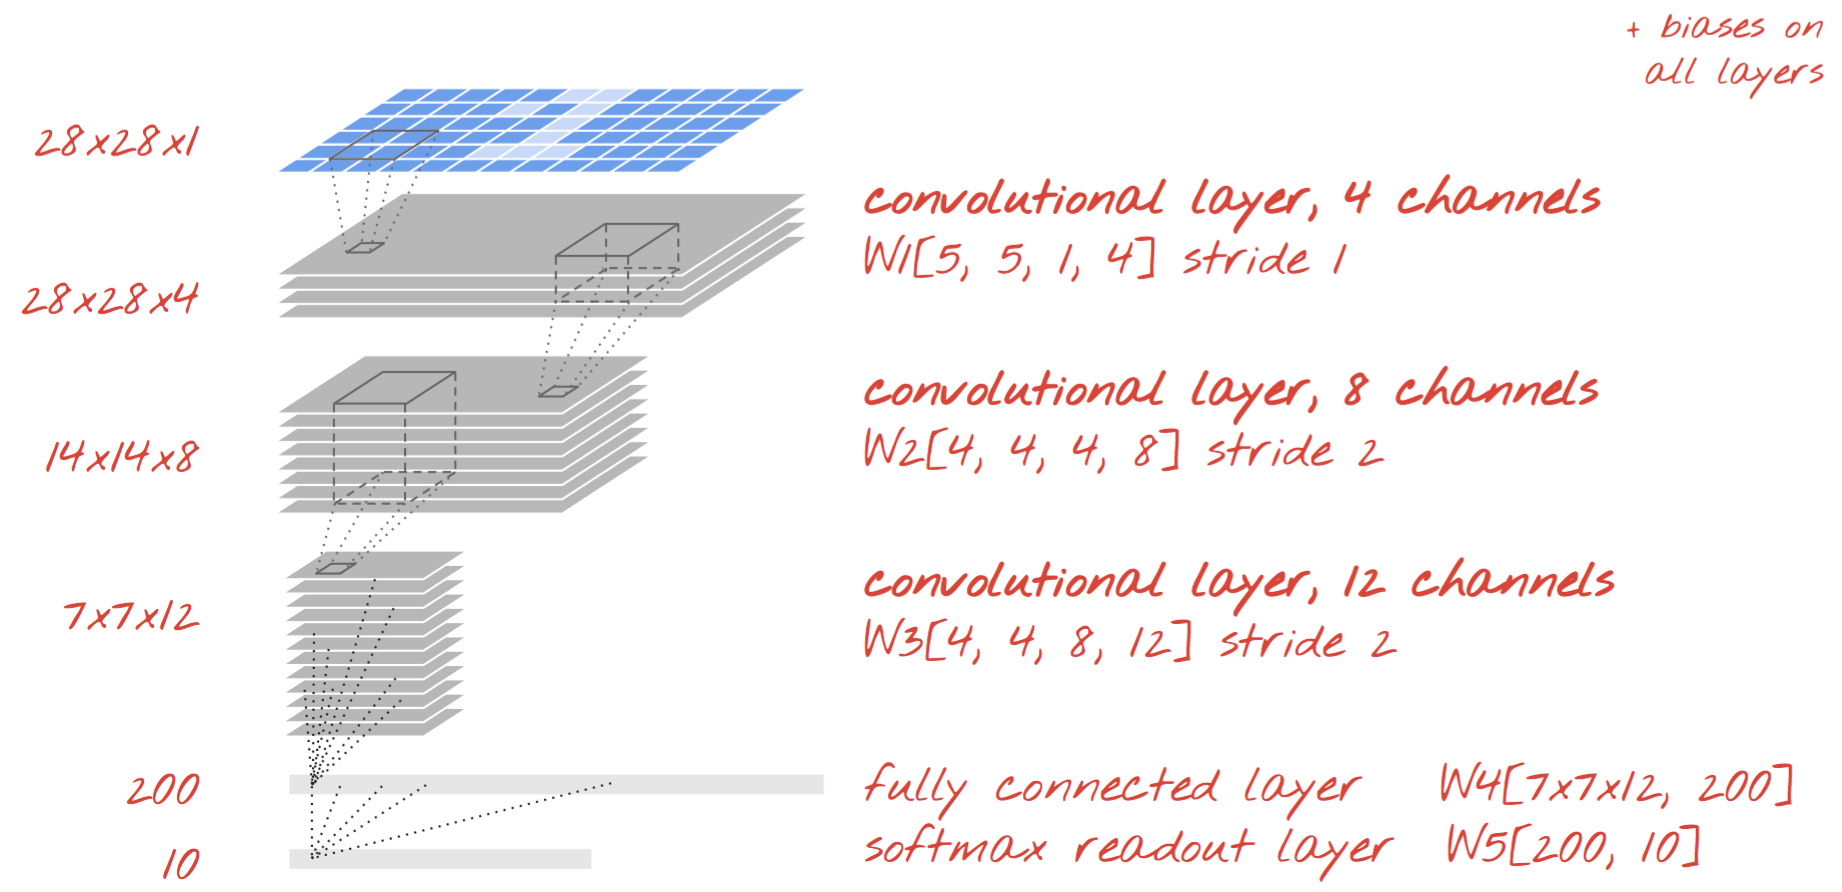
\includegraphics[width=0.9\textwidth]{figures/mnist-conv2d-1.png}
\caption{实现卷积神经网络}
 \label{fig:mnist-conv2d-1}
\end{figure}

使用\tf{}实现卷积网络,如下代码所示。

\begin{leftbar}
\begin{python}
K = 4 
L = 8
M = 12
N = 200

w1 = tf.Variable(tf.truncated_normal([5, 5, 1, K], stddev=0.1))
b1 = tf.Variable(tf.ones([K])/10)

w2 = tf.Variable(tf.truncated_normal([5, 5, K, L], stddev=0.1))
b2 = tf.Variable(tf.ones([L])/10)

w3 = tf.Variable(tf.truncated_normal([4, 4, L, M], stddev=0.1))
b3 = tf.Variable(tf.ones([M])/10)

w4 = tf.Variable(tf.truncated_normal([7 * 7 * M, N], stddev=0.1))
b4 = tf.Variable(tf.ones([N])/10)

w5 = tf.Variable(tf.truncated_normal([N, 10], stddev=0.1))
b5 = tf.Variable(tf.ones([10])/10)

y1 = tf.nn.relu(tf.nn.conv2d(
       x,  w1, strides=[1, 1, 1, 1], padding='SAME') + b1)
y2 = tf.nn.relu(tf.nn.conv2d(
       y1, w2, strides=[1, 2, 2, 1], padding='SAME') + b2)
y3 = tf.nn.relu(tf.nn.conv2d(
       y2, w3, strides=[1, 2, 2, 1], padding='SAME') + b3)

yy = tf.reshape(Y3, shape=[-1, 7 * 7 * M])
y4 = tf.nn.relu(tf.matmul(yy, w4) + b4)

logits = tf.matmul(y4, w5) + b5
y = tf.nn.softmax(logits)
\end{python}
\end{leftbar}

如\refig{mnist-conv2d-1-result}所示,经过$10^4$次训练,可以得到大约\percent{98.9}的准确率。

\begin{figure}[H]
\centering
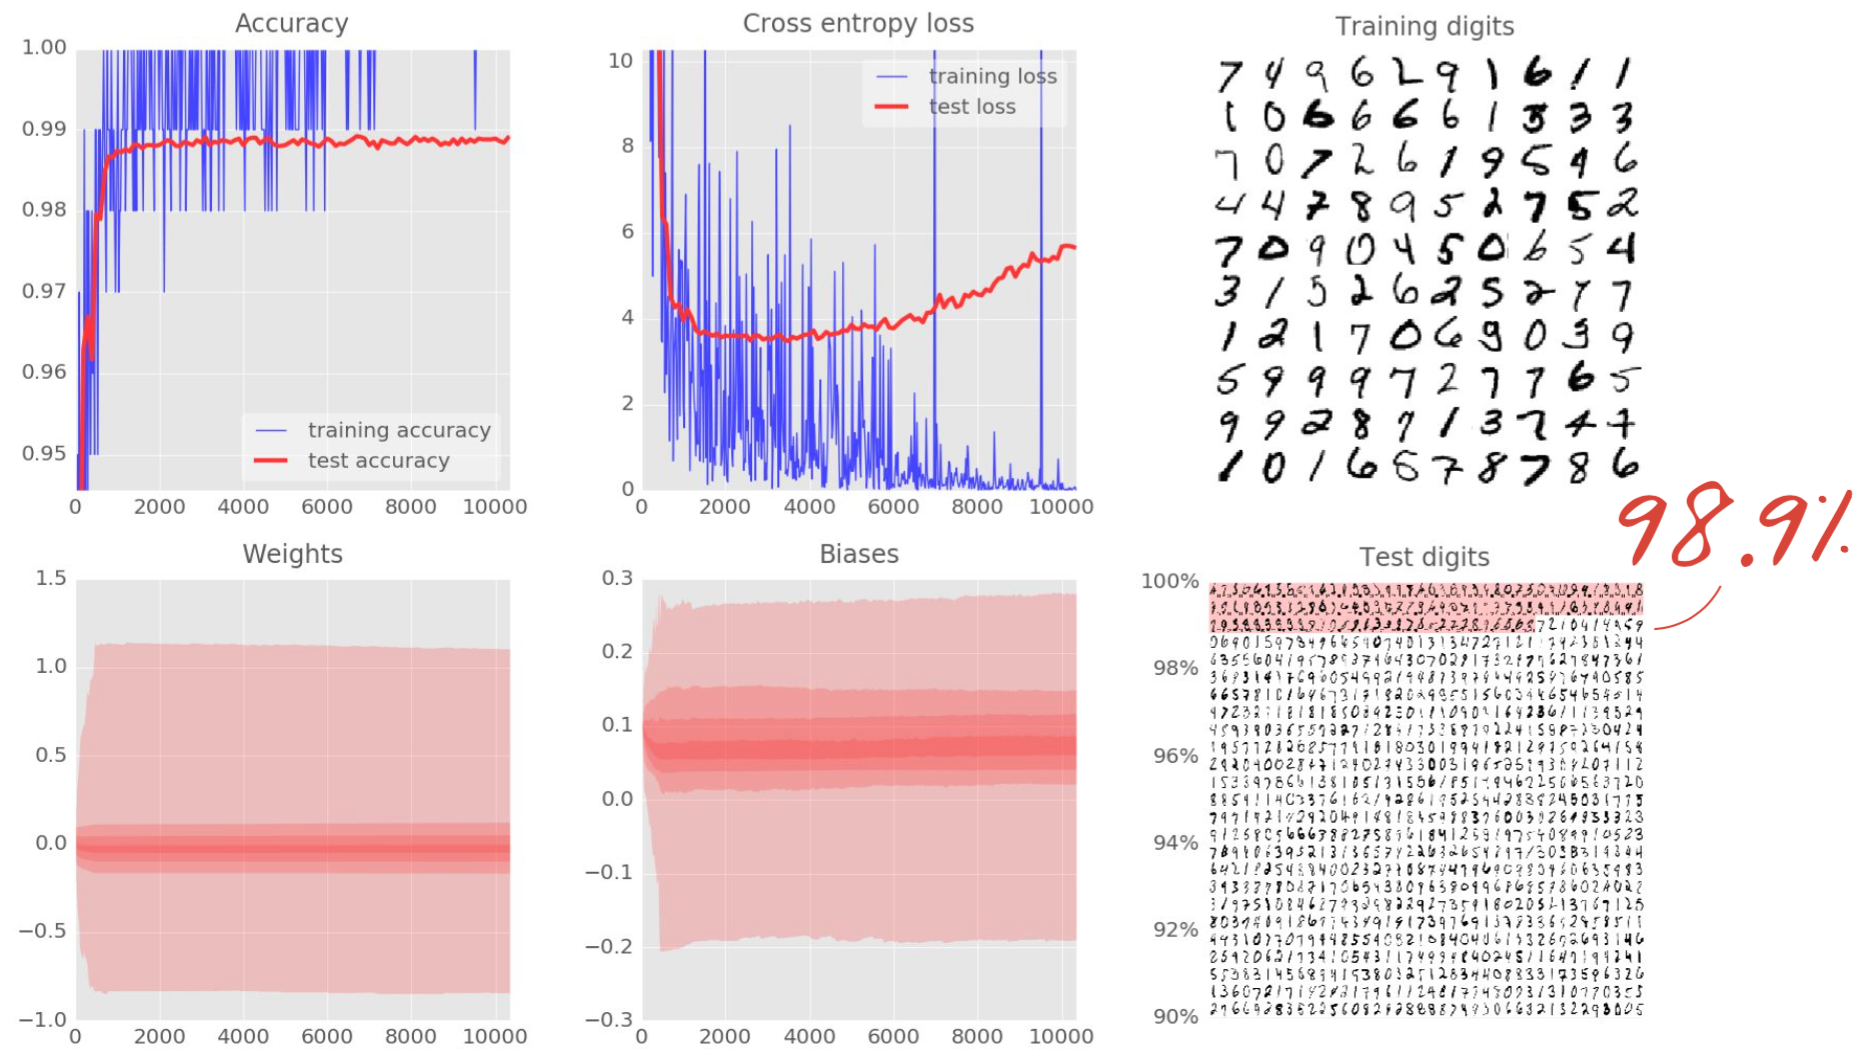
\includegraphics[width=0.9\textwidth]{figures/mnist-conv2d-1-result.png}
\caption{实现卷积网络:可以得到\percent{98.9}的准确率}
 \label{fig:mnist-conv2d-1-result}
\end{figure}

\subsection{增强卷积网络}

如\refig{mnist-conv2d-2}所示,保留之前的网络层次结构,构造了\ascii{3}个卷积层和\ascii{2}个全连接层。其中,中间隐藏层使用\ascii{ReLU}的激活函数,最后的输出层采用\ascii{softmax}的激活函数。

但是,相对于之前的卷积网络,使用了更多的通道提取更多的特征。同时,在全连接的隐藏层中实施\ascii{dropout}操作,增强网络的泛化能力。

\begin{figure}[H]
\centering
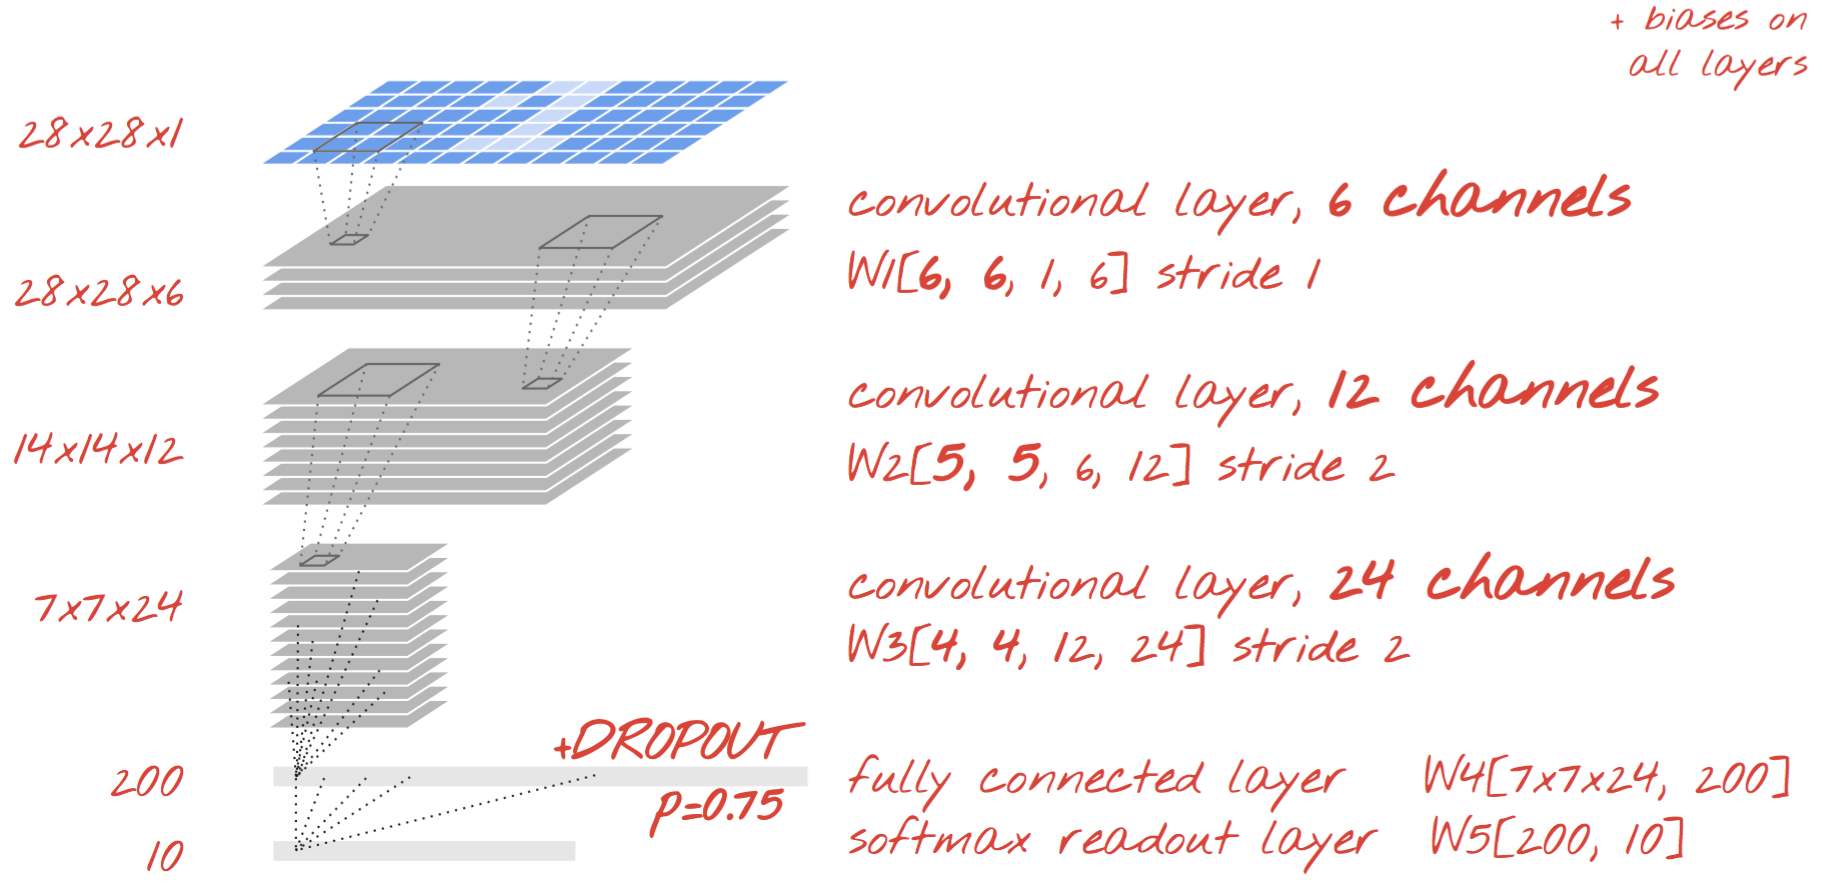
\includegraphics[width=0.9\textwidth]{figures/mnist-conv2d-2.png}
\caption{改善卷积神经网络}
 \label{fig:mnist-conv2d-2}
\end{figure}

使用\tf{}实现更大的卷积网络,如下代码所示。

\begin{leftbar}
\begin{python}
K = 6
L = 12
M = 24
N = 200

w1 = tf.Variable(tf.truncated_normal([6, 6, 1, K], stddev=0.1))
b1 = tf.Variable(tf.ones([K])/10)

w2 = tf.Variable(tf.truncated_normal([5, 5, K, L], stddev=0.1))
b2 = tf.Variable(tf.ones([L])/10)

w3 = tf.Variable(tf.truncated_normal([4, 4, L, M], stddev=0.1))
b3 = tf.Variable(tf.ones([M])/10)

w4 = tf.Variable(tf.truncated_normal([7 * 7 * M, N], stddev=0.1))
b4 = tf.Variable(tf.ones([N])/10)

w5 = tf.Variable(tf.truncated_normal([N, 10], stddev=0.1))
b5 = tf.Variable(tf.ones([10])/10)

y1 = tf.nn.relu(tf.nn.conv2d(
       x,  w1, strides=[1, 1, 1, 1], padding='SAME') + b1)
y2 = tf.nn.relu(tf.nn.conv2d(
       y1, w2, strides=[1, 2, 2, 1], padding='SAME') + b2)
y3 = tf.nn.relu(tf.nn.conv2d(
       y2, w3, strides=[1, 2, 2, 1], padding='SAME') + b3)

yy = tf.reshape(Y3, shape=[-1, 7 * 7 * M])
y4 = tf.nn.relu(tf.matmul(yy, w4) + b4)
y4d = tf.nn.dropout(y4, pkeep)

logits = tf.matmul(y4d, w5) + b5
y = tf.nn.softmax(logits)
\end{python}
\end{leftbar}

如\refig{mnist-conv2d-2-result}所示,经过$10^4$次训练,可以得到大约\percent{99.3}的准确率。

\begin{figure}[H]
\centering
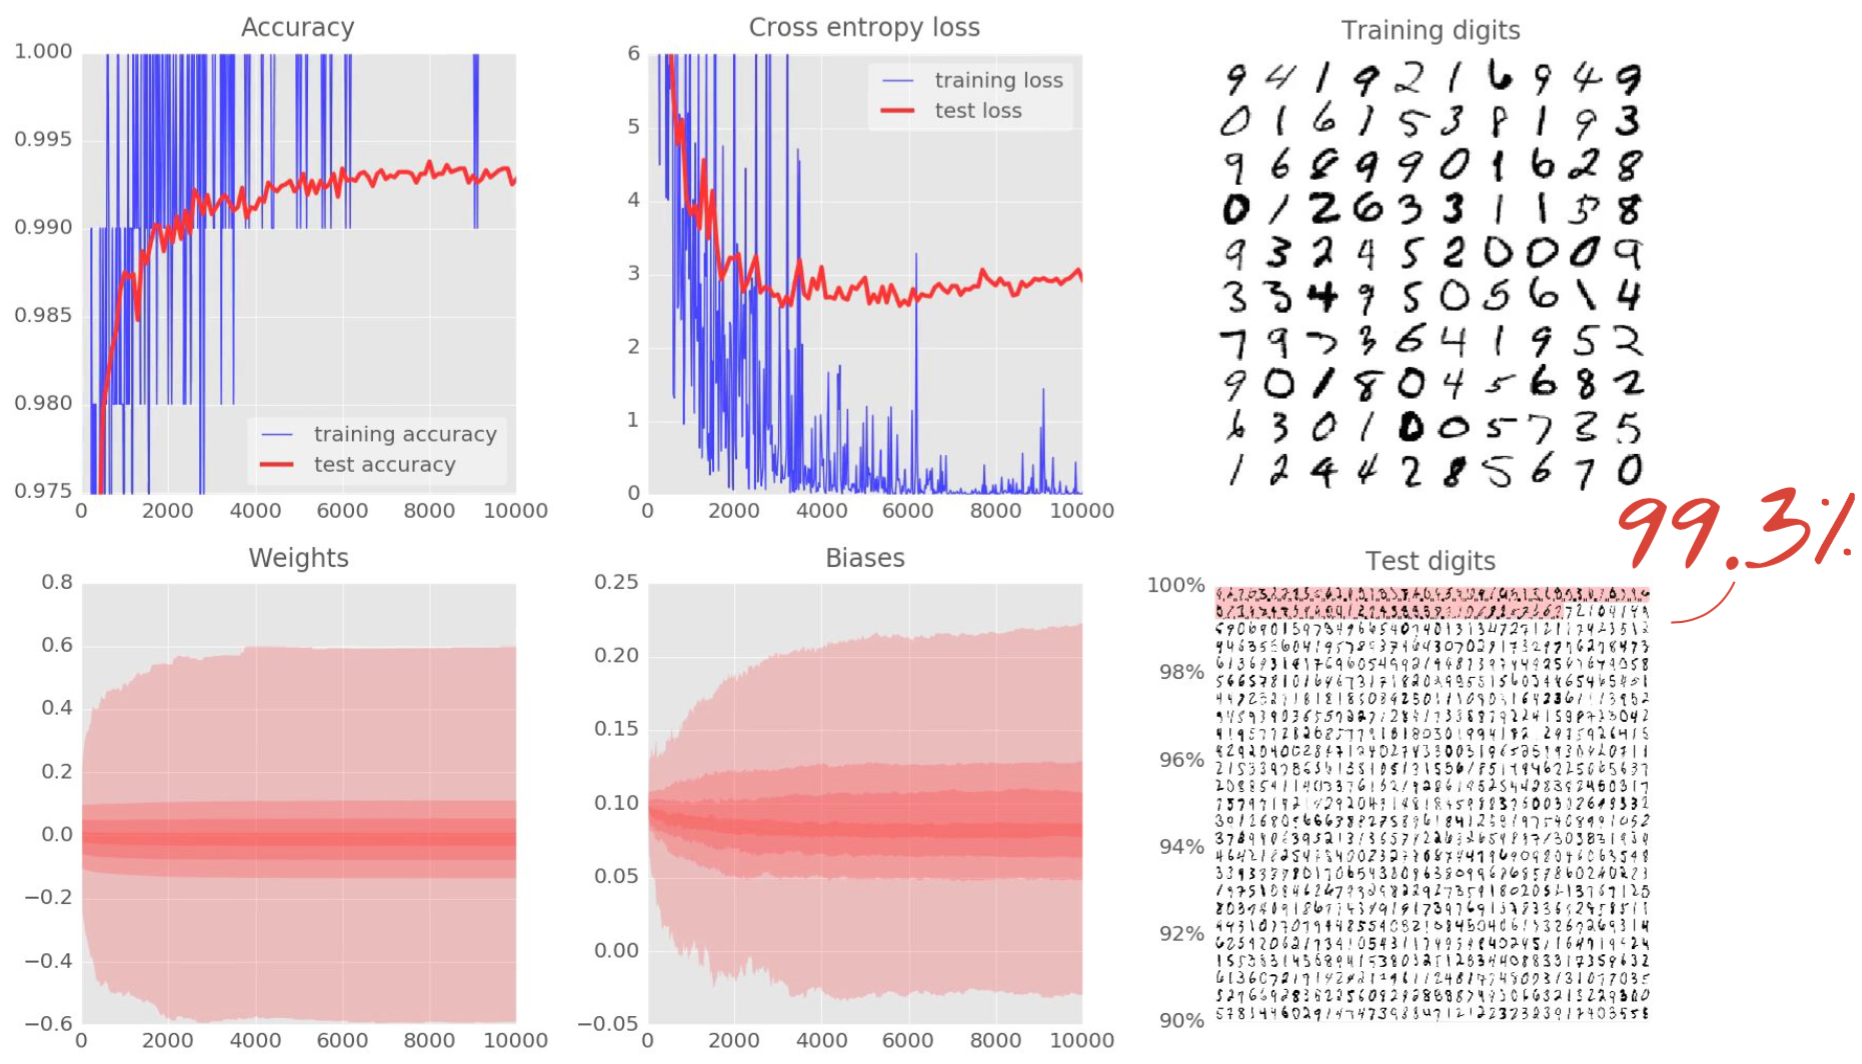
\includegraphics[width=0.9\textwidth]{figures/mnist-conv2d-2-result.png}
\caption{增强卷积网络:可以得到\percent{99.3}的准确率}
 \label{fig:mnist-conv2d-2-result}
\end{figure}

同时,相对于之前实现的卷积网络,过拟合问题得到了明显地改善,如\refig{mnist-conv2d-3-result}所示。

\begin{figure}[H]
\centering
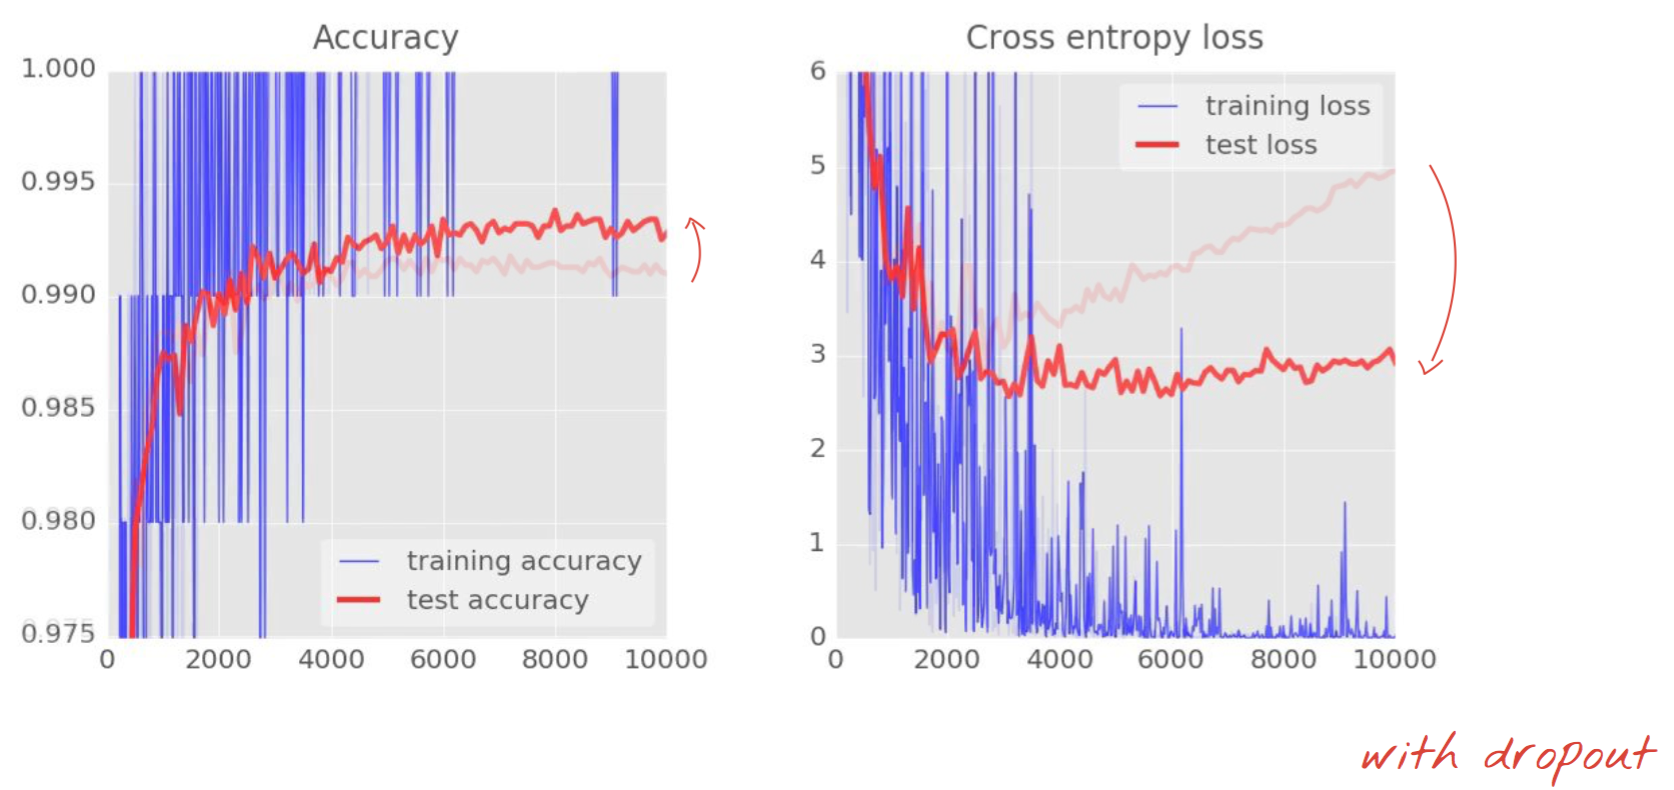
\includegraphics[width=0.9\textwidth]{figures/mnist-conv2d-3-result.png}
\caption{增强卷积网络:过拟合问题明显改善}
 \label{fig:mnist-conv2d-3-result}
\end{figure}

\end{content}

% \part{系统架构}
% \begin{savequote}[45mm]
\ascii{Any fool can write code that a computer can understand. Good programmers write code that humans can understand.}
\qauthor{\ascii{- Martin Flower}}
\end{savequote}

\chapter{系统架构} 
\label{ch:architecture}

\begin{content}

本章将阐述\tf{}的系统架构,并一个简单的例子,讲述图结构的变换过程,加深理解\tf{}运行时的工作机理。

\end{content}

\section{系统架构}

\begin{content}

\tf{}的系统结构以\ascii{C API}为界,将整个系统分为「前端」和「后端」两个子系统:

\begin{enum}
  \eitem{前端系统:提供编程模型,负责构造计算图;}
  \eitem{后端系统:提供运行时环境,负责执行计算图。} 
\end{enum}

\begin{figure}[!htbp]
\centering
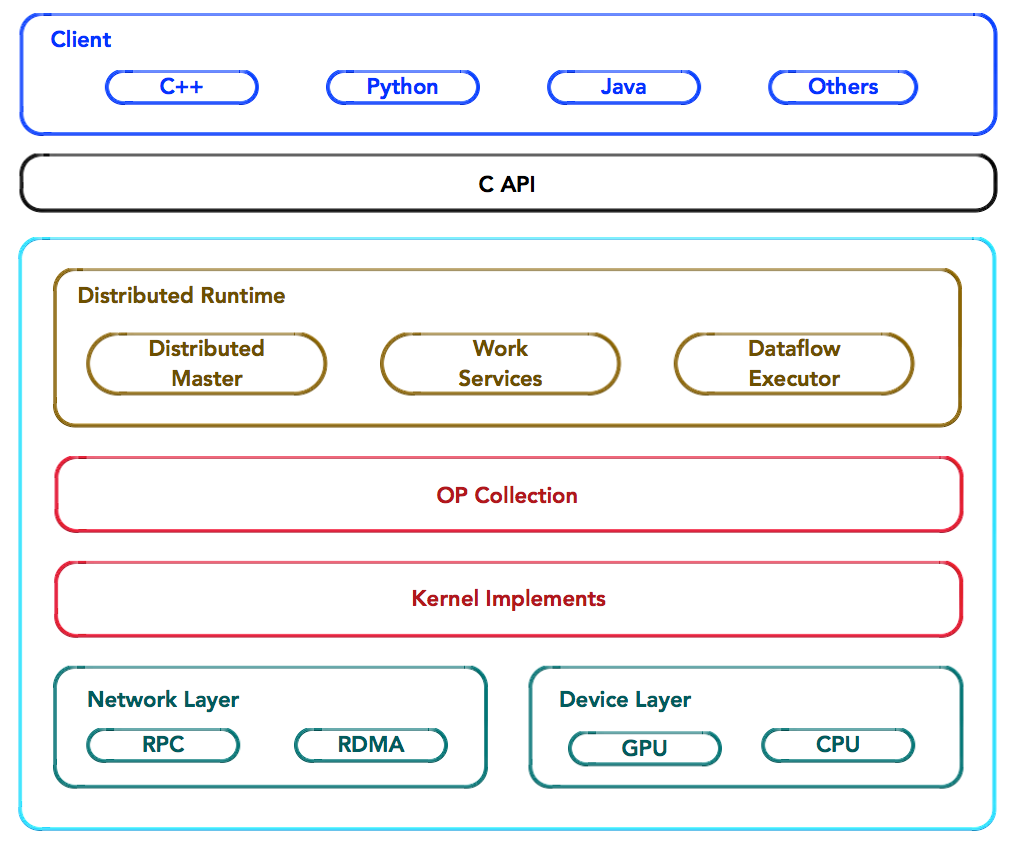
\includegraphics[width=0.9\textwidth]{figures/tf-architecture.png}
\caption{TensorFlow系统架构}
 \label{fig:tf-architecture}
\end{figure}

如\refig{tf-architecture}所示,重点关注系统中如下\ascii{4}个基本组件,它们是系统分布式运行时的核心。

\subsection{Client}

\ascii{Client}是前端系统的主要组成部分,它是一个支持多语言的编程环境。\ascii{Client}基于\ascii{TensorFlow}的编程接口,构造计算图。目前,\ascii{TensorFlow}支持\ascii{Python}和\ascii{C++}的编程接口较为完善,尤其对\ascii{Python}支持最佳;并且,对其他编程语言的编程接口的支持日益完善。

此时,\ascii{TensorFlow}并未执行任何的图计算,直至与后台计算引擎建立\ascii{Session},并以\ascii{Session}为桥梁,建立\ascii{Client}与\ascii{Master}之间的通道,将\ascii{Protobuf}格式的\ascii{GraphDef}发送至\ascii{Master},启动计算图的执行过程。

\subsection{Master}

在分布式的运行时环境中,\ascii{Client}根据\code{Session.run}传递整个计算图给后端的\ascii{Master};此时,计算图是完整的,常称为\ascii{Full Graph}。

随后,\ascii{Master}根据\ascii{Client}通过\code{Session.run}传递\code{fetches}参数列表,反向遍历\ascii{Full Graph},并按照依赖关系,对其实施剪枝,最终计算得到所依赖的「最小子图」,常称为\ascii{Client Graph}。

随后,\ascii{Master}负责将\ascii{Client Graph}按照任务的名称分裂\ascii{(split-by-task)}为多个「子图片段」,常称为\ascii{(Graph Partition)};其中,每个\ascii{Worker}对应一个\ascii{Graph Partition}。

随后,\ascii{Master}将\ascii{Graph Partition}分别注册到相应的\ascii{Worker}上,以便在不同的\ascii{Worker}上并发执行这些「子图片段」。

最后,\ascii{Master}将通知所有\ascii{Work}启动相应的\ascii{Graph Partition}的执行;其中,\ascii{Work}之间可能存在数据交互,\ascii{Master}不参与两者之间的数据交换,它们自行通信,独立交换数据即可,直至计算完成。

\subsection{Worker}

对于每以个任务,\tf{}都将启动一个\ascii{Worker}实例。\ascii{Worker}主要负责如下\ascii{3}个方面的职责:

\begin{enum}
  \eitem{处理来自\ascii{Master}的请求;}
  \eitem{调度\ascii{OP}的\ascii{Kernel}实现,执行本地子图;} 
  \eitem{协同任务之间的数据通信。}
\end{enum}

首先,\ascii{Worker}收到\ascii{Master}发送过来的图执行命令,此时的计算图相对于\ascii{Worker}是完整的,也称为\ascii{Full Graph},它对应于\ascii{Master}的一个\ascii{Graph Partition}。随后,\ascii{Worker}也会执行图剪枝,得到最小依赖的\ascii{Client Graph}。

随后,\ascii{Worker}根据当前可用的硬件环境,包括\ascii{(GPU/CPU)}资源,按照\ascii{OP}设备的约束规范,再将\ascii{Cliet Graph}分裂\ascii{(split-by-device)}为多个\ascii{Graph Partition};其中,每个计算设备对应一个\ascii{Graph Partition};随后,\ascii{Worker}启动所有当前设备的\ascii{Graph Partition}的执行。

最后,对于每一个计算设备,\ascii{Worker}将按照计算图中节点之间的依赖关系执行拓扑排序算法,并依次调用\ascii{OP}的\ascii{Kernel}实现,完成\ascii{OP}的运算(一种典型的多态实现技术)。其中,\ascii{Worker}还要负责将\ascii{OP}运算的结果发送到其他的\ascii{Work};或者接受来自其他\ascii{Worker}发送给它运算的结果,以便实现\ascii{Worker}之间的数据交互。

\subsection{Kernel}

\ascii{Kernel}是\ascii{OP}在某种硬件设备的特定实现,它负责执行\ascii{OP}的具体运算。目前,\ascii{TensorFlow}系统中包含\ascii{200}多个标准的\ascii{OP},包括数值计算,多维数组操作,控制流,状态管理等。

每一个\ascii{OP}根据设备类型都会存在一个优化了的\ascii{Kernel}实现。在运行时,运行时根据\ascii{OP}的设备约束贵方,及其本地设备的类型,为\ascii{OP}选择特定的\ascii{Kernel}实现,完成该\ascii{OP}的计算。

其中,大多数\ascii{Kernel}基于\ascii{Eigen::Tensor}实现。其中,\ascii{Eigen::Tensor}是一个使用\ascii{C++}模板技术,为多核\ascii{CPU/GPU}生成高效的并发代码。但是,\ascii{TensorFlow}也可以灵活地直接使用\ascii{cuDNN}实现更高效的\ascii{Kernel}。

此外,\ascii{TensorFlow}实现了矢量化技术,在高吞吐量、以数据为中心的应用需求中,及其移动设备中,实现更高效的推理。如果对于复合\ascii{OP}的子计算过程很难表示,或执行效率低下,\ascii{TensorFlow}甚至支持更高效的\ascii{Kernel}注册,其扩展性表现相当优越。

\end{content}

\section{图控制}

\begin{content}

随后,通过一个最简单的例子,进一步抽丝剥茧,逐渐挖掘出\tf{}计算图的控制与运行机制。


\subsection{组建集群}

如\refig{tf-1ps-1worker}所示。假如存在一个简单的分布式环境:\ascii{1 PS + 1 Worker},并将其划分为两个任务:

\begin{enum}
  \eitem{\ascii{ps0}: 使用\code{/job:ps/task:0}标记,负责模型参数的存储和更新;}
  \eitem{\ascii{worker0}: \code{/job:worker/task:0}标记,负责模型的训练。} 
\end{enum}

\begin{figure}[!htbp]
\centering
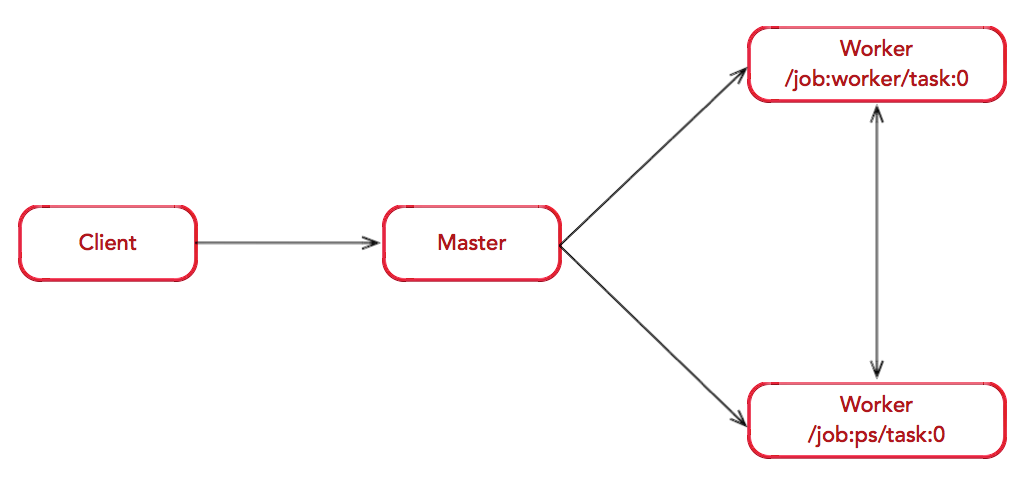
\includegraphics[width=0.9\textwidth]{figures/tf-1ps-1worker.png}
\caption{TensorFlow集群:\ascii{1 PS + 1 Worker}}
 \label{fig:tf-1ps-1worker}
\end{figure}

\subsection{图构造}

如\refig{tf-graph-construction}所示。\ascii{Client}构建了一个简单计算图;首先,将$w$与$x$进行矩阵相乘,再与截距$b$按位相加,最后更新至$s$。

\begin{figure}[!htbp]
\centering
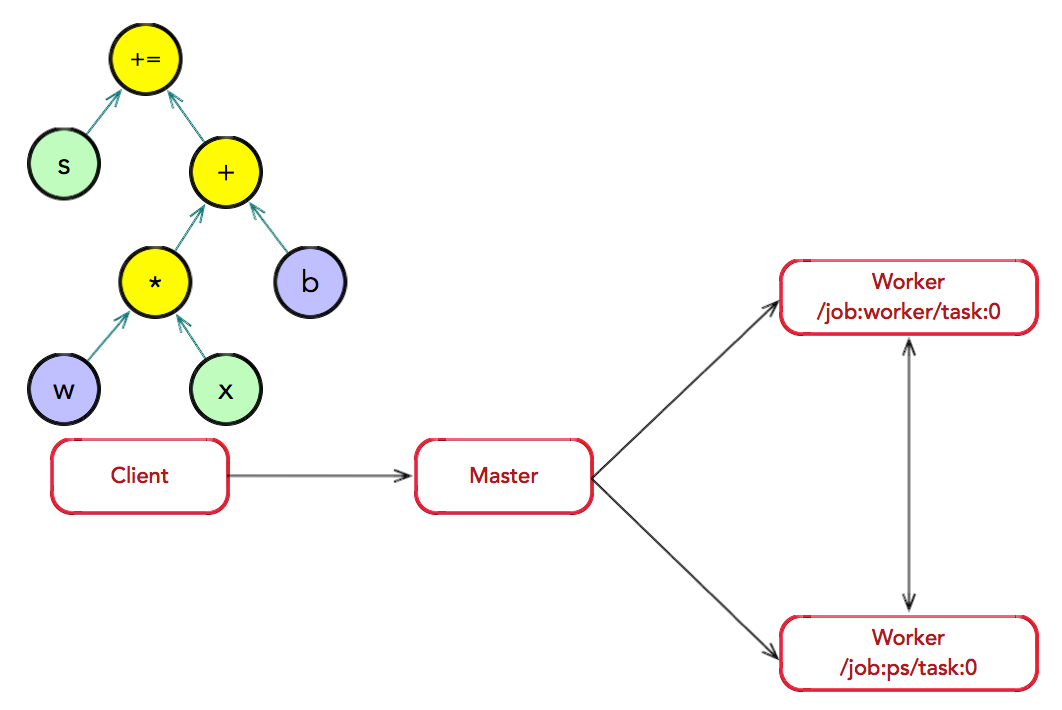
\includegraphics[width=0.9\textwidth]{figures/tf-graph-construction.png}
\caption{图构造}}
 \label{fig:tf-graph-construction}
\end{figure}

\subsection{图执行}

如\refig{tf-graph-execution}所示。首先,\ascii{Client}创建一个\code{Session}实例,建立与\ascii{Master}之间的通道;接着,\ascii{Client}通过调用\code{Sess.run}将计算图传递给\ascii{Master}。

随后,\ascii{Master}便开始启动一次\ascii{Step}的图计算过程。在执行之前,\ascii{Master}会实施一系列优化技术,例如「公共表达式消除」,「常量折叠」等。最后,\ascii{Master}负责任务之间的协同,执行优化后的计算子图。

\begin{figure}[!htbp]
\centering
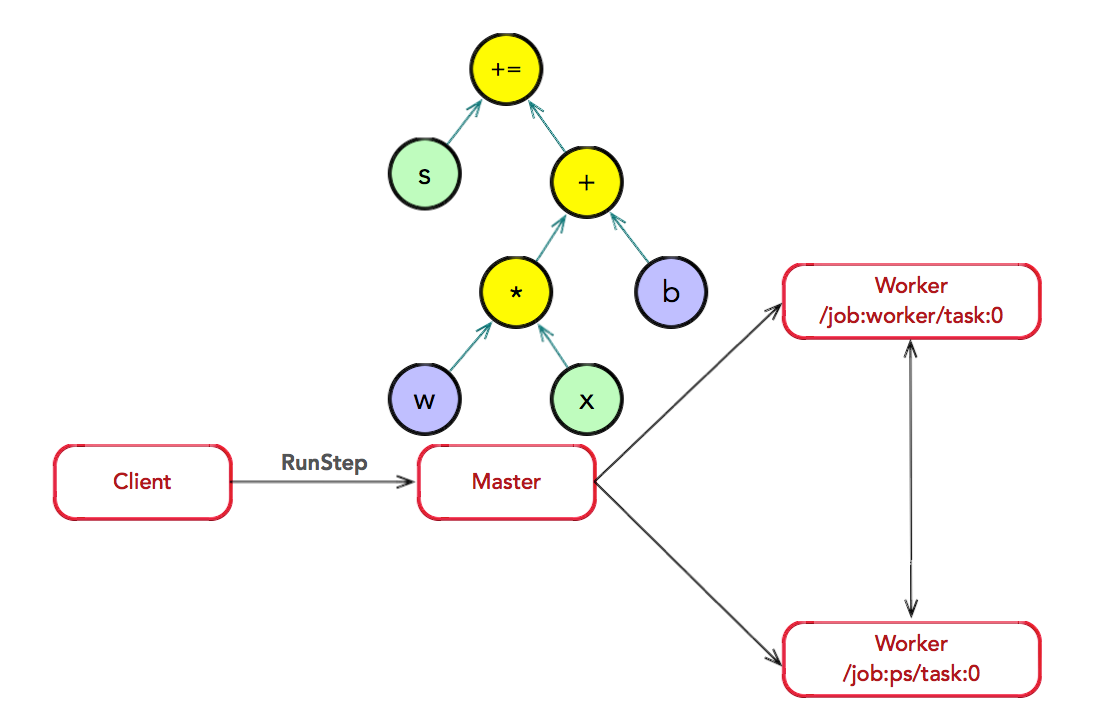
\includegraphics[width=0.9\textwidth]{figures/tf-graph-execution.png}
\caption{图执行}}
 \label{fig:tf-graph-execution}
\end{figure}

\subsubsection{图分裂}

如\refig{tf-graph-split-by-task}所示。存在一种合理的图划分算法。\ascii{Master}将模型参数相关的\ascii{OP}划分为一组,并放置在\ascii{ps0}任务上;其他\ascii{OP}划分为另外一组,放置在\ascii{worker0}任务上执行。

\begin{figure}[!htbp]
\centering
\includegraphics[width=0.9\textwidth]{figures/tf-graph-split-by-task.png}
\caption{图分裂:按任务划分}}
 \label{fig:tf-graph-split-by-task}
\end{figure}

\subsubsection{子图注册}

如\refig{tf-register-graph}所示。在图分离过程中,如果计算图的边跨越任务节点,\ascii{Master}将该边进行分裂,在两个任务之间插入\ascii{Send}和\ascii{Recv}节点,实现数据的传递。

其中,\ascii{Send}和\ascii{Recv}节点也是\ascii{OP},这是两个特殊的\ascii{OP},由内部运行时管理和控制,对用户不可见;并且,它们仅用于数据的通信,并没有任何数据计算的逻辑。

最后,\ascii{Master}通过调用\code{RegisterGraph}接口,将\ascii{Graph Partition}注册给相应的任务中,并由相应的\ascii{Worker}负责执行。

\begin{figure}[!htbp]
\centering
\includegraphics[width=0.9\textwidth]{figures/tf-register-graph.png}
\caption{子图注册:插入Send和Recv节点}}
 \label{fig:tf-register-graph}
\end{figure}

\subsubsection{子图运算}

如\refig{tf-run-graph}所示。\ascii{Master}通过调用\code{RunGraph}接口,通知所有\ascii{Worker}执行子图运算。其中,\ascii{Worker}之间通过调用\code{RecvTensor}接口,完成数据的交互。

\begin{figure}[!htbp]
\centering
\includegraphics[width=0.9\textwidth]{figures/tf-run-graph.png}
\caption{子图执行}}
 \label{fig:tf-run-graph}
\end{figure}

\end{content}













% \begin{savequote}[45mm]
\ascii{Any fool can write code that a computer can understand. Good programmers write code that humans can understand.}
\qauthor{\ascii{- Martin Flower}}
\end{savequote}

\chapter{C API:分水岭} 
\label{ch:c-api}

\begin{content}

本章通过客户端\ascii{Session}生命周期的实现为例,揭示前端\ascii{Python}与后端\cpp{}系统的实现通道,揭示\ascii{TensorFlow}多语言编程的奥秘。

\end{content}

\section{Swig:幕后英雄}

\begin{content}

前端多语言编程环境与后端\cpp{}实现系统的通道归功于\ascii{Swig}的包装器。\ascii{TensorFlow}使用\ascii{Bazel}的构建工具,在系统编译之前启动\ascii{Swig}的代码生成过程,通过\code{tensorflow.i}自动生成了两个适配(\ascii{Wrapper})文件:

\begin{enum}
  \eitem{\code{pywrap\_tensorflow\_internal.py}:  负责对接上层\ascii{Python}调用;}
  \eitem{\code{pywrap\_tensorflow\_internal.cc}: 负责对接下层\ascii{C API}调用。}
\end{enum}

如\refig{swig}所示,\code{pywrap\_tensorflow\_internal.py}模块首次被导入时,自动地加载\code{\_pywrap\_tensorflow\_internal.so}的动态链接库;其中,\code{\_pywrap\_tensorflow\_internal.so}包含了整个\tf{}运行时的所有符号。在\code{pywrap\_tensorflow\_internal.cc}的实现中,静态注册了一个函数符号表,实现了\ascii{Python}函数名到\ascii{C}函数名的二元关系。在运行时,按照\ascii{Python}的函数名称,匹配找到对应的\ascii{C}函数实现,最终实现\ascii{Python}到\code{c\_api.c}具体实现的调用关系。

\begin{figure}[H]
\centering
\includegraphics[width=1.0\textwidth]{figures/swig.png}
\caption{Swig代码生成器}
 \label{fig:swig}
\end{figure}

其中,\ascii{Bazel}的生成规则定义于\code{//tensorflow/python:pywrap\_tensorflow\_internal},如下代码所示。

\begin{leftbar}
\begin{python}
tf_py_wrap_cc(
    name = "pywrap_tensorflow_internal",
    srcs = ["tensorflow.i"],
    swig_includes = [
        "client/device_lib.i",
        "client/events_writer.i",
        "client/tf_session.i",
        "client/tf_sessionrun_wrapper.i",
        "framework/cpp_shape_inference.i",
        "framework/python_op_gen.i",
        "grappler/cost_analyzer.i",
        "grappler/model_analyzer.i",
        "grappler/tf_optimizer.i",
        "lib/core/py_func.i",
        "lib/core/strings.i",
        "lib/io/file_io.i",
        "lib/io/py_record_reader.i",
        "lib/io/py_record_writer.i",
        "platform/base.i",
        "pywrap_tfe.i",
        "training/quantize_training.i",
        "training/server_lib.i",
        "util/kernel_registry.i",
        "util/port.i",
        "util/py_checkpoint_reader.i",
        "util/stat_summarizer.i",
        "util/tfprof.i",
        "util/transform_graph.i",
    ]
)
\end{python}
\end{leftbar}

下文以客户端\ascii{Session}生命周期的实现为例,揭示前端\ascii{Python}与后端\cpp{}系统的实现通道。

\end{content}

\section{会话控制}

\begin{content}

严格意义上,\ascii{C API}并非是\ascii{Client}与\ascii{Master}的分界线。如\refig{tf-client-session}所示,\ascii{Client}存在部分\cpp{}实现,即\code{tensorflow::Session}。其中,\code{tf.Session}实例直接持有\code{tensorflow::Session}实例的句柄。在实际运行时环境中,\code{tensorflow::Session}可能存在多种实现。例如,\code{DirectSession}负责\emph{本地模式}的会话控制。而\code{GrpcSession}负责基于\ascii{gRPC}协议的\emph{分布式模式}的会话控制。一般地,用户使用的是\code{tf.Session}实施编程,而非\code{tensorflow::Session}。

\begin{figure}[!htbp]
\centering
\includegraphics[width=0.9\textwidth]{figures/tf-client-session.png}
\caption{客户端:tensorflow::Session实例创建过程}
 \label{fig:tf-client-session}
\end{figure}

\end{content}

\section{会话生命周期}

\begin{content}

会话的生命周期包括会话的创建,创建计算图,扩展计算图,执行计算图,关闭会话,销毁会话的基本过程。在前端\ascii{Python}和后端\cpp{}表现为两套相兼容的接口实现。

\subsection{Python前端}

如\refig{py-session-lifecycle}所示,在\ascii{Python}前端,\code{Session}的生命周期主要体现在:

\begin{enum}
  \eitem{创建\code{Session(target)};}
  \eitem{迭代执行\code{Session.run(fetches, feed\_dict)};}
    \begin{enum}
      \eitem{\code{Session.\_extend\_graph(graph)};}
      \eitem{\code{Session.TF\_Run(feeds, fetches, targets)};}
    \end{enum}
  \eitem{关闭\code{Session};}
  \eitem{销毁\code{Session};}
\end{enum}

\begin{figure}[H]
\centering
\includegraphics[width=0.5\textwidth]{figures/py-session-lifecycle.png}
\caption{Python: Session生命周期}
 \label{fig:py-session-lifecycle}
\end{figure}

例如,此处创建了本地模式的\code{Session}实例,并启动\code{mnist}的训练过程。

\begin{leftbar}
\begin{python}
sess = tf.Session()
for _ in range(1000):
  batch_xs, batch_ys = mnist.train.next_batch(100)
  sess.run(train_step, feed_dict={x: batch_xs, y_: batch_ys})
sess.close()
\end{python}
\end{leftbar}

\subsection{C++后端}

相应地,在\cpp{}后端,\code{Session}的生命周期主要体现在:

\begin{enum}
  \eitem{根据\code{target}多态创建\code{Session};}
  \eitem{\code{Session.Create(graph)}:有且仅有一次;}
  \eitem{\code{Session.Extend(graph)}:零次或多次;}
  \eitem{迭代执行\code{Session.Run(inputs, outputs, targets)};}
  \eitem{关闭\code{Session.Close};}
  \eitem{销毁\code{Session}对象。}
\end{enum}

\begin{figure}[H]
\centering
\includegraphics[width=0.9\textwidth]{figures/cc-session-lifecycle.png}
\caption{C++: Session生命周期}
 \label{fig:cc-session-lifecycle}
\end{figure}

例如,此处创建了本地模式的\code{DirectSession}实例,并启动计算图的执行过程。

\begin{leftbar}
\begin{c++}
// create/load graph ...
tensorflow::GraphDef graph;

// local runtime, target is ""
tensorflow::SessionOptions options;

// create Session
std::unique_ptr<tensorflow::Session> 
sess(tensorflow::NewSession(options));

// create graph at initialization.
tensorflow::Status s = sess->Create(graph);
if (!s.ok()) { ... }

// run step
std::vector<tensorflow::Tensor> outputs;
s = session->Run(
  {},               // inputs is empty
  {"output:0"},     // outputs names
  {"update_state"}, // target names
  &outputs);        // output tensors
if (!s.ok()) { ... }

// close
session->Close();
\end{c++}
\end{leftbar}

\end{content}

\section{创建会话}

\begin{content}

下面介绍Session创建的详细过程,从\ascii{Python}前端为起点,通过\ascii{Swig}自动生成的\ascii{Python-C++}的包装器,并以此为媒介,实现了\ascii{Python}到\ascii{TensorFlow}的\ascii{C API}的调用。其中,\ascii{C API}是前端系统与后端系统的分水岭。

\begin{figure}[H]
\centering
\includegraphics[width=1.0\textwidth]{figures/py-create-session.png}
\caption{创建会话}
 \label{fig:py-create-session}
\end{figure}

\subsection{编程接口}

当\ascii{Client}要启动计算图的执行过程时,先创建了一个\code{Session}实例,进而调用父类\code{BaseSession}的构造函数。

\begin{leftbar}
\begin{python}[caption={tensorflow/python/client/session.py}]
class Session(BaseSession):
  def __init__(self, target='', graph=None, config=None):
    super(Session, self).__init__(target, graph, config=config)
    self._default_graph_context_manager = None
    self._default_session_context_manager = None
\end{python}
\end{leftbar}

在\code{BaseSession}的构造函数中,将调用\code{pywrap\_tensorflow}模块中的函数。其中,\code{TF\_NewDeprecatedSession}是遗留下来的,已被废弃的接口实现。在新的\ascii{API}中,直接将图实例传递给后端\ascii{C++},避免了前后端图实例序列化的开销。

\begin{leftbar}
\begin{python}[caption={tensorflow/python/client/session.py}]
from tensorflow.python import pywrap_tensorflow as tf_session

class BaseSession(SessionInterface):
  def __init__(self, target='', graph=None, config=None):
    # default graph
    if graph is None:
      self._graph = ops.get_default_graph()
    else:
      self._graph = graph

    # handle to tensorflow::Session
    self._session = None
    opts = tf_session.TF_NewSessionOptions(target=self._target, 
                                           config=config)
    try:
      with errors.raise_exception_on_not_ok_status() as status:
        if self._created_with_new_api:
          self._session = tf_session.TF_NewSession(
              self._graph._c_graph, opts, status)
        else:
          self._session = tf_session.TF_NewDeprecatedSession(opts, status)
    finally:
      tf_session.TF_DeleteSessionOptions(opts)
\end{python}
\end{leftbar}

如\refig{tf-graph-inst}所示,\code{ScopedTFGraph}是对\code{TF\_Graph}的包装器,完成类似于\ascii{C++}的\ascii{RAII}的工作机制。而\code{TF\_Graph}持有\code{ternsorflow::Graph}实例。其中,\code{self.\_graph.\_c\_graph}返回一个\code{TF\_Graph}实例,后者通过\ascii{C API}创建的图实例。

\begin{leftbar}
\begin{python}[caption={tensorflow/python/framework/ops.py}]
class Graph(object):
  def __init__(self):
    if _USE_C_API:
      self._scoped_c_graph = c_api_util.ScopedTFGraph()
    else:
      self._scoped_c_graph = None

  def _c_graph(self):
    if self._scoped_c_graph:
      return self._scoped_c_graph.graph
    return None
\end{python}
\end{leftbar}

\begin{leftbar}
\begin{python}[caption={tensorflow/python/framework/c\_api\_util.py}]
class ScopedTFGraph(object):
  def __init__(self):
    self.graph = c_api.TF_NewGraph()

  def __del__(self):
    if c_api.TF_DeleteGraph is not None:
      c_api.TF_DeleteGraph(self.graph)
\end{python}
\end{leftbar}

\begin{figure}[H]
\centering
\includegraphics[width=0.3\textwidth]{figures/tf-graph-inst.png}
\caption{前后端:图实例传递}
 \label{fig:tf-graph-inst}
\end{figure}

\subsubsection{Python包装器}

在\code{pywrap\_tensorflow}模块中,通过\code{\_pywrap\_tensorflow\_internal}的转发,实现了从\ascii{Python}到动态连接库\code{\_pywrap\_tensorflow\_internal.so}的函数调用。

\begin{leftbar}
\begin{python}[caption={tensorflow/bazel-bin/tensorflow/python/pywrap\_tensorflow\_internal.py}]
def TF_NewDeprecatedSession(opts, status):
  return _pywrap_tensorflow_internal.TF_NewDeprecatedSession(opts, status)

def TF_NewSession(graph, opts, status):
  return _pywrap_tensorflow_internal.TF_NewSession(graph, opts, status)
\end{python}
\end{leftbar}

\subsubsection{C++包装器}

在\code{pywrap\_tensorflow\_internal.cc}的具体实现中,静态注册了函数调用的符号表,实现\ascii{Python}的函数名称到\cpp{}函数实现的具体映射。

\begin{leftbar}
\begin{c++}[caption={tensorflow/bazel-bin/tensorflow/python/pywrap\_tensorflow\_internal.cc}]
static PyMethodDef SwigMethods[] = {
  // ...
  { (char *)"TF_NewDeprecatedSession", 
    _wrap_TF_NewDeprecatedSession, METH_VARARGS, NULL},

  { (char *)"TF_NewSession", 
    _wrap_TF_NewSession, METH_VARARGS, NULL},
};
\end{c++}
\end{leftbar}

最终,\code{\_wrap\_TF\_NewSession/\_wrap\_TF\_NewDeprecatedSession}将分别调用\code{c\_api.h}对其开放的\ascii{API}接口:\code{TF\_NewSession/TF\_NewDeprecatedSession}。也就是说,自动生成的\code{pywrap\_tensorflow\_internal.cc}仅仅负责\ascii{Python}函数到\ascii{C/C++}函数调用的转发,最终将调用底层\ascii{C}系统向上提供的\ascii{API}接口。

\subsection{C API}

\code{c\_api.h}是\ascii{TensorFlow}的后端执行系统面向前端开放的公共\ascii{API}接口。其中,新的接口实现采用了引用计数的技术,实现图实例在多个\code{Session}实例中共享。

\begin{leftbar}
\begin{c++}[caption={tensorflow/c/c\_api.c}]
TF_Session* TF_NewSession(TF_Graph* graph, const TF_SessionOptions* opt,
                          TF_Status* status) {
  Session* session;
  status->status = NewSession(opt->options, &session);
  if (status->status.ok()) {
    if (graph != nullptr) {
      mutex_lock l(graph->mu);
      graph->num_sessions += 1;
    }
    return new TF_Session(session, graph);
  } else {
    return nullptr;
  }
}

TF_DeprecatedSession* TF_NewDeprecatedSession(const TF_SessionOptions* opt,
                                              TF_Status* status) {
  Session* session;
  status->status = NewSession(opt->options, &session);
  if (status->status.ok()) {
    return new TF_DeprecatedSession({session});
  } else {
    DCHECK_EQ(nullptr, session);
    return nullptr;
  }
}
\end{c++}
\end{leftbar}

\subsection{后端系统}

\code{NewSession}将根据前端传递的\code{target},使用\code{SessionFactory}多态创建不同类型的\code{tensorflow::Session}实例。

\begin{leftbar}
\begin{c++}[caption={tensorflow/c/c\_api.c}]
Status NewSession(const SessionOptions& options, Session** out_session) {
  SessionFactory* factory;
  Status s = SessionFactory::GetFactory(options, &factory);
  if (!s.ok()) {
    *out_session = nullptr;
    return s;
  }
  *out_session = factory->NewSession(options);
  if (!*out_session) {
    return errors::Internal("Failed to create session.");
  }
  return Status::OK();
}
\end{c++}
\end{leftbar}

\subsubsection{工厂方法}

在后端\cpp{}实现中,\code{tensorflow::Session}的创建使用了抽象工厂方法。如果\code{SessionOptions}中的\code{target}为空字符串(默认的),则创建\code{DirectSession}实例,启动本地运行模式;如果\code{SessionOptions}中的\code{target}以\code{grpc://}开头,则创建\code{GrpcSession}实例,启动基于\code{RPC}的分布式运行模式。如\refig{cc-session-factory}所示。

\begin{figure}[H]
\centering
\includegraphics[width=1.0\textwidth]{figures/cc-session-factory.png}
\caption{tensorflow::Session创建:抽象工厂方法}
 \label{fig:cc-session-factory}
\end{figure}

\end{content}

\section{创建/扩展图}

\begin{content}

在既有的接口实现中,需要将图构造期构造好的图序列化,并传递给后端\ascii{C++}系统。而在新的接口实现中,无需实现图的创建或扩展。因为在创建\ascii{OP}时,节点实时添加至后端\ascii{C++}系统的图实例中。但是,既有接口实现,对于理解系统行为较为重要,在次做简单地阐述。

\ascii{Python}前端将迭代调用\code{Session.run}接口,将构造好的计算图,以\code{GraphDef}的形式发送给\cpp{}后端。其中,前端每次调用\code{Session.run}接口时,都会试图将新增节点的计算图发送给后端系统,以便将新增节点的计算图\ascii{Extend}到原来的计算图中。特殊地,在首次调用\code{Session.run}时,将发送整个计算图给后端系统。

后端系统首次调用\code{Session.Extend}时,转调(或等价实现)\code{Session.Create}。以后,后端系统每次调用\code{Session.Extend}时将真正执行\code{Extend}的语义,将新增的计算图的节点追加至原来的计算图中。

\begin{figure}[H]
\centering
\includegraphics[width=0.9\textwidth]{figures/py-session-create-graph.png}
\caption{创建图}
 \label{fig:py-session-create-graph}
\end{figure}

\subsection{编程接口}

在既有的接口实现中,通过\code{\_extend\_graph}实现图实例的扩展。

\begin{leftbar}
\begin{python}[caption={tensorflow/python/client/session.py}]
class Session(BaseSession):
  def run(self, fetch_list, feed_dict=None, options=None, run_metadata=None):
    # ignores implements...
    self._extend_graph()
    # ignores implements...

\end{python}
\end{leftbar}

在首次调用\code{self.\_extend\_graph}时,或者有新的节点被添加至计算图中时,对计算图\code{GraphDef}实施序列化操作,最终触发\code{tf\_session.TF\_ExtendGraph}的调用。

\begin{leftbar}
\begin{python}[caption={tensorflow/python/client/session.py}]
from tensorflow.python import pywrap_tensorflow as tf_session

class Session(BaseSession):
  def _extend_graph(self):
    if self._created_with_new_api: return

    with self._extend_lock:
      if self._graph.version > self._current_version:
        graph_def, self._current_version = self._graph._as_graph_def(
            from_version=self._current_version,
            add_shapes=self._add_shapes)

        with errors.raise_exception_on_not_ok_status() as status:
          tf_session.TF_ExtendGraph(
              self._session, graph_def.SerializeToString(), status)
\end{python}
\end{leftbar}

\subsubsection{Python包装器}

\begin{leftbar}
\begin{python}[caption={tensorflow/bazel-bin/tensorflow/python/pywrap\_tensorflow\_internal.py}]
def TF_ExtendGraph(sess, graph_def, status):
  return _pywrap_tensorflow.TF_ExtendGraph(sess, graph_def, status)
\end{python}
\end{leftbar}

\subsubsection{C++包装器}

\begin{leftbar}
\begin{c++}[caption={tensorflow/bazel-bin/tensorflow/python/pywrap\_tensorflow\_internal.cc}]
static PyMethodDef SwigMethods[] = {
  // ignore implements...
  { (char *)"TF_ExtendGraph", 
    _wrap_TF_ExtendGraph, METH_VARARGS, NULL},
};
\end{c++}
\end{leftbar}

\subsection{C API}

\code{TF\_ExtendGraph}是\ascii{C API}对接上层编程环境的接口。首先,它完成计算图\code{GraphDef}的反序列化,最终调用\code{tensorflow::Session}的\code{Extend}接口。

\begin{leftbar}
\begin{c++}[caption={tensorflow/c/c\_api.c}]
void TF_ExtendGraph(TF_DeprecatedSession* sess, 
  const void* proto, size_t proto_len, TF_Status* status) {
  GraphDef g;
  if (!tensorflow::ParseProtoUnlimited(&g, proto, proto_len)) {
    status->status = InvalidArgument("Invalid GraphDef");
    return;
  }
  status->status = sess->session->Extend(g);
}
\end{c++}
\end{leftbar}

\subsection{后端系统}

\code{tensorflow::Session}在运行时根据\code{Session}的动态类型,将多态地调用相应子类的实现。

\begin{leftbar}
\begin{c++}[caption={tensorflow/core/common\_runtime/session.h}]
class Session {
public:
  virtual Status Create(const GraphDef& graph) = 0;
  virtual Status Extend(const GraphDef& graph) = 0;
};
\end{c++}
\end{leftbar}

其中,\code{Create}表示在当前的\code{tensorflow::Session}实例上注册计算图,如果要注册新的计算图,需要关闭该\code{tensorflow::Session}对象。\code{Extend}表示在\code{tensorflow::Session}实例上已注册的计算图上追加节点。\code{Extend}首次执行时,等价于\code{Create}的语义,因为首次\code{Extend}时,已注册的计算图为空。事实上,系统就是按照如上方案实现的,此处以\code{GrpcSession}实现为例。

\subsubsection{首次扩展图: GrpcSession}

如果判断引用\code{Master}的\code{handle}不为空,则执行\code{Extend};否则,执行\code{Create}的语义,建立与\code{Master}的连接,并持有\code{MasterSession}的\code{handle}。

\begin{leftbar}
\begin{c++}[caption={tensorflow/core/distributed\_runtime/rpc/grpc\_session.cc}]
Status GrpcSession::Extend(const GraphDef& graph) {
  CallOptions call_options;
  call_options.SetTimeout(options_.config.operation_timeout_in_ms());
  return ExtendImpl(&call_options, graph);
}

Status GrpcSession::ExtendImpl
  (CallOptions* call_options, const GraphDef& graph) {
  if (handle_is_empty()) {
    // Session was unitialized, 
    // so simply initialize the session with 'graph'.
    return Create(graph);
  }
  // ignore implements...  
}
\end{c++}
\end{leftbar}

\end{content}

\section{迭代运行}

\begin{content}

如\refig{py-session-run}所示,\ascii{Python}前端\code{Session.run}实现将\code{fetches, feed\_dict}传递给后端系统,后端系统调用\code{Session.Run}接口。后端系统的一次\code{Session.Run}执行常常被称为一次\ascii{Step}。其中,\ascii{Step}的执行过程是\ascii{TensorFlow}运行时的关键路径。

\begin{figure}[H]
\centering
\includegraphics[width=1.0\textwidth]{figures/py-session-run.png}
\caption{迭代执行}
 \label{fig:py-session-run}
\end{figure}

\subsection{编程接口}

当\ascii{Client}调用\code{Session.run}时,最终会调用\code{pywrap\_tensorflow\_internal}模块中的函数。

\begin{leftbar}
\begin{python}[caption={tensorflow/python/client/session.py}]
from tensorflow.python import pywrap_tensorflow as tf_session

class Session(BaseSession):
  def run(self, fetch_list, feed_dict=None, options=None, run_metadata=None):
    # ignores other implements...
    self._extend_graph()
    with errors.raise_exception_on_not_ok_status() as status:
      if self._created_with_new_api:
        return tf_session.TF_SessionRun_wrapper(
            session, options, feed_dict, fetch_list, target_list,
            run_metadata, status)
      else:
        return tf_session.TF_Run(session, options,
                                 feed_dict, fetch_list, target_list,
                                 status, run_metadata)
\end{python}
\end{leftbar}


\subsubsection{Python包装器}

\begin{leftbar}
\begin{python}[caption={tensorflow/bazel-bin/tensorflow/python/pywrap\_tensorflow\_internal.py}]
def TF_SessionRun_wrapper(session, run_options, inputs, 
  outputs, targets, run_metadata, out_status):
  return _pywrap_tensorflow_internal.TF_SessionRun_wrapper(
    session, run_options, inputs, outputs, targets, run_metadata, out_status)

def TF_Run(sess, options, feeds, outputs, 
  targets, status, run_metadata):
  return _pywrap_tensorflow.TF_Run(
    sess, options, feeds, outputs, targets, status, run_metadata)
\end{python}
\end{leftbar}

\subsubsection{C++包装器}

\begin{leftbar}
\begin{c++}[caption={tensorflow/bazel-bin/tensorflow/python/pywrap\_tensorflow\_internal.cc}]
static PyMethodDef SwigMethods[] = {
  // ...
  { (char *)"TF_Run", 
    _wrap_TF_Run, METH_VARARGS, NULL},

  { (char *)"TF_SessionRun_wrapper", 
    _wrap_TF_SessionRun_wrapper, METH_VARARGS, NULL},
};
\end{c++}
\end{leftbar}

最终,\code{\_wrap\_TF\_Run/\_wrap\_TF\_SessionRun\_wrapper}将分别转调\ascii{C API}对应的\code{TF\_Run/TF\_SessionRun}接口函数。

\subsection{C API}

在既有的接口中,\code{TF\_Run}是\ascii{C API}对接上层编程环境的接口。首先,它完成输入数据从\ascii{C}到\cpp{}的格式转换,并启动后台的\code{tensorflow::Session}的执行过程。当执行完成后,再将\code{outputs}的输出数据从\cpp{}到\ascii{C}的格式转换。\code{TF\_SessionRun}与\code{TF\_Run}工作机制差不多,在此不再冗述。

\begin{leftbar}
\begin{c++}[caption={tensorflow/c/c\_api.c}]
void TF_Run(TF_DeprecatedSession* s, 
  // session options
  const TF_Buffer* run_options,
  // Input tensors
  const char** c_input_names, TF_Tensor** c_inputs, int ninputs,
  // Output tensors
  const char** c_output_names, TF_Tensor** c_outputs, int noutputs,
  // Target nodes
  const char** c_target_oper_names, int ntargets,
  // run\_metadata
  TF_Buffer* run_metadata, TF_Status* status) {
  // convert data format, ignore implements...
  s->session->Run(options_proto, input_names, output_names,
                  target_names, &outputs, &run_metadata); 
  // store results in c\_outputs...
}

void TF_SessionRun(TF_Session* session, 
  const TF_Buffer* run_options,
  // Input tensors
  const TF_Output* inputs, TF_Tensor* const * input_values, int ninputs, 
  // Output tensors
  const TF_Output* outputs, TF_Tensor** output_values, int noutputs,
  // Target nodes
  const TF_Operation* const* target_opers, int ntargets,
  // run\_metadata
  TF_Buffer* run_metadata, TF_Status* status) {
  // ignore implements.
}
\end{c++}
\end{leftbar}

\subsection{后端系统}

\code{tensorflow::Session}在运行时按照其动态类型,将多态地调用相应的子类实现。

\begin{leftbar}
\begin{c++}[caption={tensorflow/core/common\_runtime/session.h}]
class Session {
public:
  virtual Status Run(
    const RunOptions& options,
    const vector<pair<string, Tensor> >& inputs,
    const vector<string>& output_names,
    const vector<string>& target_names,
    vector<Tensor>* outputs, RunMetadata* run_metadata) {
      return errors::Unimplemented(
        "Run with options is not supported for this session.");
  }
};
\end{c++}
\end{leftbar}

输入包括:

\begin{enum}
  \eitem{\code{options}:\code{Session}的运行配置参数;}
  \eitem{\code{inputs}: 输入\code{Tensor}的名字列表;}
  \eitem{\code{output\_names}: 输出\code{Tensor}的名字列表;}
  \eitem{\code{targets}: 无输出,待执行的\ascii{OP}的名字列表。} 
\end{enum}

输出包括:

\begin{enum}
  \eitem{\code{outputs}: 输出的\code{Tensor}列表;}
  \eitem{\code{run\_metadata}: 运行时元数据的收集器。}
\end{enum}

其中,输出的\code{outputs}列表与输入的\code{output\_names}一一对应,如果运行时因并发执行,导致\code{outputs}乱序执行,最终返回时需要对照输入的\code{output\_names}名字列表,对\code{outputs}进行排序。

\end{content}

\section{关闭会话}

\begin{content}

当计算图执行完毕后,需要关闭\code{tf.Session},以便释放后端的系统资源,包括队列,\ascii{IO}等。会话关闭流程较为简单,如\refig{py-session-close}所示。。

\begin{figure}[H]
\centering
\includegraphics[width=0.9\textwidth]{figures/py-session-close.png}
\caption{关闭会话}
 \label{fig:py-session-close}
\end{figure}

\subsection{编程接口}

当\ascii{Client}调用\code{Session.close}时,最终会调用\code{pywrap\_tensorflow}模块中的函数: \code{TF\_CloseDeprecatedSession}。

\begin{leftbar}
\begin{python}[caption={tensorflow/python/client/session.py}]
from tensorflow.python import pywrap_tensorflow as tf_session

class Session(BaseSession):
  def close(self):
    if self._created_with_new_api:
      if self._session and not self._closed:
        self._closed = True
        with errors.raise_exception_on_not_ok_status() as status:
          tf_session.TF_CloseSession(self._session, status)
    else:
      with self._extend_lock:
        if self._opened and not self._closed:
          self._closed = True
          with errors.raise_exception_on_not_ok_status() as status:
            tf_session.TF_CloseDeprecatedSession(self._session, status)
\end{python}
\end{leftbar}

\subsubsection{Python包装器}

\begin{leftbar}
\begin{python}[caption={tensorflow/bazel-bin/tensorflow/python/pywrap\_tensorflow\_internal.py}]
def TF_CloseSession(sess, status):
    return _pywrap_tensorflow_internal.TF_CloseSession(sess, status)

def TF_CloseDeprecatedSession(sess, status):
  return _pywrap_tensorflow.TF_CloseDeprecatedSession(sess, status)
\end{python}
\end{leftbar}

\subsubsection{C++包装器}

\code{\_wrap\_TF\_CloseSession/\_wrap\_TF\_CloseDeprecatedSession}将分别转调\ascii{C API}对应的\code{TF\_CloseSession/TF\_CloseDeprecatedSession}接口函数。

\begin{leftbar}
\begin{c++}[caption={tensorflow/bazel-bin/tensorflow/python/pywrap\_tensorflow\_internal.cc}]
static PyMethodDef SwigMethods[] = {
  // ...
  { (char *)"TF_CloseSession", 
    _wrap_TF_CloseSession, METH_VARARGS, NULL},

  { (char *)"TF_CloseDeprecatedSession", 
    _wrap_TF_CloseDeprecatedSession, METH_VARARGS, NULL},
};
\end{c++}
\end{leftbar}

\subsection{C API}

\code{TF\_CloseSession/TF\_CloseDeprecatedSession}直接完成\code{tensorflow::Session}的关闭操作。

\begin{leftbar}
\begin{c++}[caption={tensorflow/c/c\_api.c}]
void TF_CloseSession(TF_Session* s, TF_Status* status) {
  status->status = s->session->Close();
}

void TF_CloseDeprecatedSession(TF_DeprecatedSession* s, TF_Status* status) {
  status->status = s->session->Close();
}
\end{c++}
\end{leftbar}

\subsection{后端系统}

\code{Session(C++)}在运行时其动态类型,将多态地调用相应的子类实现。

\begin{leftbar}
\begin{c++}[caption={tensorflow/core/common\_runtime/session.h}]
class Session {
public:
  virtual Status Close() = 0;
};
\end{c++}
\end{leftbar}

\end{content}

\section{销毁会话}

\begin{content}

当\code{tf.Session}不在被使用,由\ascii{Python}的\ascii{GC}释放。\code{Session.\_\_del\_\_}被调用后,将启动后台\code{tensorflow::Session}对象的析构过程。如\refig{py-delete-session}所示。

\begin{figure}[H]
\centering
\includegraphics[width=0.9\textwidth]{figures/py-delete-session.png}
\caption{销毁会话}
 \label{fig:py-delete-session}
\end{figure}

\subsection{编程接口}

当\ascii{Client}调用\code{Session.\_\_del\_\_}时,先启动\code{Session.close}的调用,最终会调用\code{pywrap\_tensorflow}模块中的函数\code{TF\_DeleteSession/TF\_DeleteDeprecatedSession}。

\begin{leftbar}
\begin{python}[caption={tensorflow/python/client/session.py}]
from tensorflow.python import pywrap_tensorflow as tf_session

class Session(BaseSession):
  def __del__(self):
    # 1. close session unconditionally.
    try:
      self.close()
    except Exception:
      pass
    # 2. delete session unconditionally.
    if self._session is not None:
      try:
        status = c_api_util.ScopedTFStatus()
        if self._created_with_new_api:
          tf_session.TF_DeleteSession(self._session, status)
        else:
          tf_session.TF_DeleteDeprecatedSession(self._session, status)
      except AttributeError:
        pass
      self._session = None
\end{python}
\end{leftbar}

\subsubsection{Python包装器}

\begin{leftbar}
\begin{python}[caption={tensorflow/bazel-bin/tensorflow/python/pywrap\_tensorflow\_internal.py}]
def TF_DeleteSession(sess, status):
    return _pywrap_tensorflow_internal.TF_DeleteSession(sess, status)

def TF_DeleteDeprecatedSession(sess, status):
  return _pywrap_tensorflow.TF_DeleteDeprecatedSession(sess, status)
\end{python}
\end{leftbar}

\subsubsection{C++包装器}

\code{\_wrap\_TF\_DeleteSession/\_wrap\_TF\_DeleteDeprecatedSession}将分别转调\ascii{C API}对应的\code{TF\_DeleteSession/TF\_DeleteDeprecatedSession}接口函数。

\begin{leftbar}
\begin{c++}[caption={tensorflow/bazel-bin/tensorflow/python/pywrap\_tensorflow\_internal.cc}]
static PyMethodDef SwigMethods[] = {
  // ...
  { (char*)"TF_DeleteSession", 
    _wrap_TF_DeleteSession, METH_VARARGS, NULL},

  { (char*)"TF_DeleteDeprecatedSession", 
    _wrap_TF_DeleteDeprecatedSession, METH_VARARGS, NULL},
};
\end{c++}
\end{leftbar}

\subsection{C API}

\code{TF\_DeleteDeprecatedSession}直接完成\code{tensorflow::Session}对象的释放。而新的接口\code{TF\_DeleteSession}实现中,当需要删除\code{tensorflow::Session}实例时,相应的图实例的计数器减\ascii{1}。当计数器为\ascii{0}时,则删除该图实例;否则,不删除该图实例。

\begin{leftbar}
\begin{c++}[caption={tensorflow/c/c\_api.c}]
void TF_DeleteSession(TF_Session* s, TF_Status* status) {
  status->status = Status::OK();
  TF_Graph* const graph = s->graph;
  if (graph != nullptr) {
    graph->mu.lock();
    graph->num_sessions -= 1;
    const bool del = graph->delete_requested && graph->num_sessions == 0;
    graph->mu.unlock();
    if (del) delete graph;
  }
  delete s->session;
  delete s;
}

void TF_DeleteDeprecatedSession(TF_DeprecatedSession* s, TF_Status* status) {
  status->status = Status::OK();
  delete s->session;
  delete s;
}
\end{c++}
\end{leftbar}

\subsection{后端系统}

\code{tensorflow::Session}在运行时其动态类型,多态地调用相应子类实现的析构函数。

\begin{leftbar}
\begin{c++}[caption={tensorflow/core/common\_runtime/session.h}]
class Session {
public:
  virtual ~Session() {};
};
\end{c++}
\end{leftbar}

\end{content}

\section{性能调优}

\begin{content}

相比遗留的接口实现,新的接口实现存在若干优化技术提升系统的性能。虽然,截止本书撰写时,新的接口并未完全对外发布,但可以预期未来将删除既有已废弃的接口,替换为了新的接口实现。

\subsection{共享图实例}

如\refig{tf-graph-session-relation}所示,一个\code{Session}只能运行一个图实例。如果一个\code{Session}要运行其他的图实例,必须先关掉\code{Session},然后再将新的图实例注册到此\code{Session}中,最后启动新的计算图的执行过程。

但反过来,一个计算图可以运行在多个\code{Session}实例上。如果在\code{Graph}实例上维持\code{Session}的引用计数器,在\code{Session}创建时,在该图实例上增加\ascii{1};在\code{Session}销毁时(不是关闭\code{Session}),在该图实例上减少\ascii{1};当计数器为\ascii{0}时,则自动删除图实例。在新的接口实现中,实现了该引用计数器的技术。

\begin{figure}[H]
\centering
\includegraphics[width=0.7\textwidth]{figures/tf-graph-session-relation.png}
\caption{计算图:Session引用计数器技术}
 \label{fig:tf-graph-session-relation}
\end{figure}

\subsection{消除序列化}

如\refig{tf-old-session-interface}所示,在遗留的接口实现中,前端\ascii{Python}在图构造期,将图构造完成后,并将其序列化,最后通过\code{Session::Create}或\code{Session::Extend}传递给后端\ascii{C++}系统。这本质是一个图实例的拷贝过程,具有很大的时延开销。

\begin{figure}[H]
\centering
\includegraphics[width=0.8\textwidth]{figures/tf-old-session-interface.png}
\caption{图实例:序列化/反序列化}
 \label{fig:tf-old-session-interface}
\end{figure}

如\refig{tf-new-session-interface}所示,在新的接口实现中,可以去除\code{Session}的\code{Create/Extend}的语义。在图的构造器,前端\ascii{Python}在构造每个\ascii{OP}时,直接通过\ascii{C API}将其追加至后端\ascii{C++}的图实例中,从而避免了图实例在前后端的序列化和反序列化的开销。

\begin{figure}[H]
\centering
\includegraphics[width=0.8\textwidth]{figures/tf-new-session-interface.png}
\caption{图实例:实施注册ascii{OP}}
 \label{fig:tf-new-session-interface}
\end{figure}

\end{content}


% \part{编程模型}
% \begin{savequote}[45mm]
\ascii{Any fool can write code that a computer can understand. Good programmers write code that humans can understand.}
\qauthor{\ascii{- Martin Flower}}
\end{savequote}

\chapter{计算图} 
\label{ch:computation-graph}

\begin{content}

在\tf{}的计算图中,使用\ascii{OP}表示节点,根据\ascii{OP}之间计算和数据依赖关系,构造\ascii{OP}之间生产与消费的数据依赖关系,并通过有向边表示。

其中,有向边存在两种类型,一种承载数据,并使用\code{Tensor}表示;另一种不承载数据,仅表示计算依赖关系。

本章将阐述\tf{}中最重要的领域对象:计算图。为了全面阐述计算图的关键实现技术,将分别探讨前后端的系统设计和实现,并探究前后端系统间计算图转换的工作流原理。

\end{content}

\section{Python前端}

\begin{content}

在\ascii{Python}的前端系统中,并没有\code{Node, Edge}的概念,仅存在\code{Operation, Tensor}的概念。事实上,在前端\ascii{Python}系统中,\code{Operation}表示图中的\code{Node}实例,而\code{Tensor}表示图中的\code{Edge}实例。

\subsection{Operation}

\code{Operation}表示某种抽象计算,它以零个或多个\code{Tensor}作为输入,经过计算后,输出零个或多个\code{Tensor}。

如\refig{py-operation}所示。在计算图构造期间,通过\ascii{OP}构造器\ascii{(OP Constructor)},构造\code{Operation}实例,并将其注册至默认的图实例中;与此同时,\code{Operation}反过来通过\ascii{graph}直接持有该图实例。

\code{Operation}的元数据由\code{OpDef}与\code{NodeDef}持有,它们以\ascii{ProtoBuf}的格式存在,它描述了\code{Operation}最本质的东西。其中,\code{OpDef}描述了\code{OP}的静态属性信息,例如名称,输入输出的属性名等信息。而\code{NodeDef}描述了\ascii{OP}的动态属性值信息。

\code{Operation}根据上游节点的输出,经过计算输出到下游。其中,\code{Operation}的输入和输出以\code{Tensor}的形式存在。从而上下游产生了数据依赖关系。

此外,\code{Operation}可能持有上游的控制依赖边的集合,表示其潜在的计算依赖关系。

\begin{figure}[!htbp]
\centering
\includegraphics[width=0.9\textwidth]{figures/py-operation.png}
\caption{领域对象:Operation}
 \label{fig:py-operation}
\end{figure}

\subsection{Tensor}

一个\code{Tensor}表示\code{Operation}的某个输出的符号句柄,它并不持\code{Operation}输出的真实数据。可以通过\code{Session.run}计算得到\code{Tensor}所持有的真实数据。

如\refig{py-tensor}所示。\code{Tensor}是两个\code{Operation}数据交换的桥梁,它们之间构造了典型的「生产者-消费者」的关系。

\begin{figure}[!htbp]
\centering
\includegraphics[width=0.9\textwidth]{figures/py-tensor.png}
\caption{领域对象:Tensor}
 \label{fig:py-tensor}
\end{figure}

其中,\code{Tensor}通过\ascii{op}持有扮演生产者角色的\code{Operation},并且使用\code{index}表示该\code{Tensor}在该\code{Operation}输出列表中的索引。也就是说,可以使用\code{op:index}的二元组信息在图中唯一标识一个\code{Tensor}实例。

此外,\code{Tensor}持有\code{Operation}的消费者列表。计算图以\code{Tensor}为边,构建\code{Operation}之间的数据连接,从而实现了整个计算图的数据依赖构建。

\subsubsection{生产者与消费者}

如\refig{py-tensor-producter-consumer}所示。上游\code{Operation}作为生产者,经过某种抽象计算,生产了一个\code{Tensor},并以此作为该上游\code{Operation}的输出之一,并使用\code{index}标识。

该\code{Tensor}被传递给下游\code{Operation},并作为下游\code{Operation}的输入,下游\code{Operation}充当该\code{Tensor}的消费者。

\begin{figure}[!htbp]
\centering
\includegraphics[width=0.9\textwidth]{figures/py-tensor-producter-consumer.png}
\caption{Tensor: 生产者-消费者关系}
 \label{fig:py-tensor-producter-consumer}
\end{figure}

\subsubsection{建立关联}

最后,参看\code{Operation}与\code{Tensor}的部分实现,很容易找两者「生产者-消费者」的关联关系。当\code{Tensor}列表作为输入流入\code{Operation}时,此时建立了下游\code{Operation}与输入的\code{Tensor}列表之间的消费关系。

\begin{leftbar}
\begin{python}
class Operation(object):
  def __init__(self, node_def, graph, inputs=None, output_types=None):
    # \_inputs as consumers
    self._inputs = list(inputs)
    for a in self._inputs:
      a._add_consumer(self)

    # self as producer
    self._output_types = output_types
    self._outputs = [Tensor(self, i, output_type)
                     for i, output_type in enumerate(output_types)]
\end{python}
\end{leftbar}


同样地,\code{Tensor}在构造函数中持有作为上游的的生产者\code{Operation},及其它在该\code{Operation}的\code{outputs}列表中的索引。此外,当调用\code{\_add\_consumer},将该下游\code{Operation}追加至消费者列表之中。

\begin{leftbar}
\begin{python}
class Tensor(_TensorLike):
  def __init__(self, op, value_index, dtype):    
    # Index of the OP's endpoint that produces this tensor.
    self._op = op
    self._value_index = value_index
    
    # List of operations that use this Tensor as input.  
    # We maintain this list to easily navigate a computation graph.
    self._consumers = []

  def _add_consumer(self, consumer):
    if not isinstance(consumer, Operation):
      raise TypeError("Consumer must be an Operation: %s" % consumer)
    self._consumers.append(consumer)
\end{python}
\end{leftbar}

\subsection{Graph}

如\refig{py-graph}所示。一个\code{Graph}对象将包含一系列\code{Operation}对象,表示计算单元的集合;同时,它间接持有一系列\code{Tensor}对象,表示数据单元的集合。

\begin{figure}[!htbp]
\centering
\includegraphics[width=0.9\textwidth]{figures/py-graph.png}
\caption{领域对象:Graph}
 \label{fig:py-graph}
\end{figure}

\subsection{图构造}

在计算图的构造期间,不执行任何\ascii{OP}的计算。简单地说,图的构造过程就是根据\ascii{OP}构造器完成\code{Operation}实例的构造。而在\code{Operation}实例的构造之前,需要实现完成\code{OpDef}与\code{NodeDef}的构造过程。

\subsubsection{OpDef仓库}

\code{OpDef}仓库在系统首次访问时,实现了\code{OpDef}的延迟加载和注册。也就是说,对于某中类型的\code{OpDef}仓库,\code{\_InitOpDefLibrary}模块首次导入时,扫描\code{op\_list\_ascii}表示的所有\ascii{OP},并将其转换为\ascii{Protobuf}格式的\code{OpList}实例,最终将其注册到\code{OpDefLibrary}实例之中。

例如,模块\code{gen\_array\_ops}是构建版本时自动生成的,它主要完成所有\code{array\_ops}类型的\code{OpDef}的定义,并自动注册到\code{OpDefLibrary}的仓库实例中,并提供按名查找\code{OpDef}的服务接口。

\begin{leftbar}
\begin{python}
_op_def_lib = _InitOpDefLibrary()

def _InitOpDefLibrary():
  op_list = _op_def_pb2.OpList()
  _text_format.Merge(_InitOpDefLibrary.op_list_ascii, op_list)   
  op_def_lib = _op_def_library.OpDefLibrary()
  op_def_lib.add_op_list(op_list)
  return op_def_lib

_InitOpDefLibrary.op_list_ascii = """op {
  name: "ZerosLike"
  input_arg {
    name: "x"
    type_attr: "T"
  }
  output_arg {
    name: "y"
    type_attr: "T"
  }
  attr {
    name: "T"
    type: "type"
  }
}
# ignore others
"""
\end{python}
\end{leftbar}

\subsubsection{工厂方法}

如\refig{py-op-factory-and-repo}所示。当\ascii{Client}使用\ascii{OP}构造器创建一个\code{Operation}实例时,将最终调用\code{Graph.create\_op}方法,将该\code{Operation}实例注册到该图实例中。

也就是说,一方面,\code{Graph}充当\code{Operation}的工厂,负责\code{Operation}的创建职责;另一方面,\code{Graph}充当\code{Operation}的仓库,负责\code{Operation}的存储,检索,转换等操作。

这个过程常称为计算图的构造。在计算图的构造期间,并不会触发运行时的\ascii{OP}运算,它仅仅描述计算节点之间的依赖关系,并构建\ascii{DAG}图,对整个计算过程做整体规划。

\begin{figure}[!htbp]
\centering
\includegraphics[width=0.9\textwidth]{figures/py-op-factory-and-repo.png}
\caption{Graph: OP工厂 + OP仓库}
 \label{fig:py-op-factory-and-repo}
\end{figure}

\subsubsection{OP构造器}

如\refig{py-op-constructor}所示。在图构造期,\ascii{Client}使用\code{tf.zeros\_like}构造一个名为\code{ZerosLike}的\ascii{OP},该\ascii{OP}拥有一个输入,输出一个全\ascii{0}的\ascii{Tensor};其中,\code{tf.zeros\_like}常称为\ascii{OP}构造器。

然后,\ascii{OP}构造器调用一段自动生成的代码,进而转调\code{OpDefLibrary.apply\_op}方法。

\begin{figure}[!htbp]
\centering
\includegraphics[width=0.9\textwidth]{figures/py-op-constructor.png}
\caption{OP构造器与代码生成器}
 \label{fig:py-op-constructor}
\end{figure}

\subsubsection{构造OpDef与NodeDef}

然后,如\refig{py-graph-create-op}所示。\code{OpDefLibrary}根据\ascii{OP}的名字从\code{OpDefLibrary}中,找到对应\code{OpDef}实例;最终,通过\code{Graph.create\_op}的工厂方法,创建\code{NodeDef}实例,进而创建\code{Operation}实例,将其自身注册到图实例中。

\begin{figure}[!htbp]
\centering
\includegraphics[width=0.9\textwidth]{figures/py-graph-create-op.png}
\caption{创建Operation实例: 创建OpDef, NodeDef实例}
 \label{fig:py-graph-create-op}
\end{figure}

\end{content}

\section{后端C++}

\begin{content}

在\ascii{C++}后端,计算图是\ascii{TensorFlow}领域模型的核心。

\subsection{边}

\code{Edge}持有前驱节点与后驱节点,从而实现了计算图的连接。一个节点可以拥有零条或多条输入边,与可以有零条或多条输出边。一般地,计算图中存在两类边:

\begin{enum}
  \eitem{普通边:用于承载数据(以\code{Tensor}表示),表示节点间“生产者-消费者”的数据依赖关系,常用实线表示;}
  \eitem{控制依赖:不承载数据,用于表示节点间的执行依赖关系,常用虚线表示。} 
\end{enum}

\subsubsection{两个标识}

\ascii{Edge}持有两个重要的索引:

\begin{enum}
  \eitem{\code{src\_output}:表示该边为「前驱节点」的第\code{src\_output}条输出边;}
  \eitem{\code{dst\_input}:表示该边为「后驱节点」的第\code{dst\_input}条输入边。} 
\end{enum}


\begin{figure}[!htbp]
\centering
\includegraphics[width=0.9\textwidth]{figures/cc-edge-model.png}
\caption{领域对象:Edge}
 \label{fig:cc-edge-model}
\end{figure}

例如,存在两个前驱节点\code{s1, s2},都存在两条输出边;存在两个后驱节点\code{d1, d2},都存在两条输入边。

\begin{figure}[!htbp]
\centering
\includegraphics[width=0.9\textwidth]{figures/cc-edge-model-example.png}
\caption{边例子}
 \label{fig:cc-edge-model-example}
\end{figure}

\subsubsection{控制依赖}

对于控制依赖边,其\code{src\_output, dst\_input}都为\code{-1(Graph::kControlSlot)},暗喻控制依赖边不承载任何数据。

\begin{leftbar}
\begin{c++}
bool Edge::IsControlEdge() const {
   // or dst\_input\_ == Graph::kControlSlot;
   return src_output_ == Graph::kControlSlot;
}
\end{c++}
\end{leftbar}

\subsubsection{Tensor标识}

一般地,计算图的「普通边」承载\code{Tensor},并使用\code{TensorId}标识。\code{Tensor}标识由源节点的名字,及其所在边的\code{src\_output}唯一确定。

\begin{leftbar}
\begin{c++}
TensorId ::= node_name:src_output
\end{c++}
\end{leftbar}

缺省地,\code{src\_output}默认为\ascii{0};也就是说,\code{node\_name}与\code{node\_name:0}两者等价。特殊地,当\code{src\_output}等于\ascii{-1}时,表示该边为「控制依赖边」,\code{TensorId}可以标识为\code{\^node\_name},标识该边依赖于\code{node\_name}所在的节点。

\subsection{节点}

\code{Node}(节点)可以拥有零条或多条输入/输出的边,并使用\code{in\_edges, out\_edges}分别表示输入边和输出边的集合。另外,\code{Node}持有\code{NodeDef, OpDef}。其中,\code{NodeDef}包含设备分配信息,及其\ascii{OP}的属性值列表;\code{OpDef}持有\ascii{OP}的元数据,包括\ascii{OP}输入输出类型等信息。

\begin{figure}[!htbp]
\centering
\includegraphics[width=0.9\textwidth]{figures/cc-node-model.png}
\caption{领域对象:Node}
 \label{fig:cc-node-model}
\end{figure}

\subsubsection{输入边}

在输入边的集合中,可以按照索引\code{(dst\_input)}线性查找。当节点输入的边比较多时,可能会成为性能的瓶颈。依次类推,按照索引\code{(src\_output)}查找输出边,算法类同。

\begin{leftbar}
\begin{c++}
Status Node::input_edge(int idx, const Edge** e) const {
  for (auto edge : in_edges()) {
    if (edge->dst_input() == idx) {
      *e = edge;
      return Status::OK();
    }
  }
  return errors::NotFound("not found input edge ", idx);
}
\end{c++}
\end{leftbar}

\subsubsection{前驱节点}

首先通过\code{idx}索引找到输入边,然后通过输入边找到前驱节点。依次类推,按照索引查找后驱节点,算法类同。

\begin{leftbar}
\begin{c++}
Status Node::input_node(int idx, const Node** n) const {
  const Edge* e = nullptr;
  TF_RETURN_IF_ERROR(input_edge(idx, &e));
  *n = e == nullptr ? nullptr : e->src();
  return Status::OK();
}
\end{c++}
\end{leftbar}

\subsection{图}

\code{Graph}(计算图)就是节点与边的集合。计算图是一个\ascii{DAG}图,计算图的执行过程将按照\ascii{DAG}的拓扑排序,依次启动\ascii{OP}的运算。其中,如果存在多个入度为\ascii{0}的节点,\ascii{TensorFlow}运行时可以实现并发,同时执行多个\ascii{OP}的运算,提高执行效率。

\begin{figure}[!htbp]
\centering
\includegraphics[width=0.9\textwidth]{figures/cc-graph-model.png}
\caption{领域模型:图}
 \label{fig:cc-graph-model}
\end{figure}

\subsubsection{空图}

计算图的初始状态,并非是一个空图。实现添加了两个特殊的节点:\code{Source}与\code{Sink}节点,分别表示\ascii{DAG}图的起始节点与终止节点。其中,\code{Source}的\code{id}为\ascii{0},\code{Sink}的\code{id}为\ascii{1};依次论断,普通\ascii{OP}节点的\ascii{id}将大于\ascii{1}。

\code{Source}与\code{Sink}之间,通过连接「控制依赖」的边,保证计算图的执行始于\code{Source}节点,终于\code{Sink}节点。它们之前的控制依赖边,其\code{src\_output, dst\_input}值都为\ascii{-1}。

\begin{figure}[!htbp]
\centering
\includegraphics[width=0.9\textwidth]{figures/cc-empty-graph.png}
\caption{空图}
 \label{fig:cc-empty-graph}
\end{figure}

\code{Source}与\code{Sink}是两个内部实现保留的节点,其节点名称以下划线开头,分别使用\code{\_SOURCE}和\code{\_SINK}命名;并且,它们都是\code{NoOp},表示不执行任何计算。

\begin{leftbar}
\begin{c++}
Node* Graph::AddInternalNode(const char* name, int id) {
  NodeDef def;
  def.set_name(name);
  def.set_op("NoOp");

  Status status;
  Node* node = AddNode(def, &status);
  TF_CHECK_OK(status);
  CHECK_EQ(node->id(), id);
  return node;
}

Graph::Graph(const OpRegistryInterface* ops)
    : ops_(ops), arena_(8 << 10 /* 8kB */) {
  auto src  = AddInternalNode("_SOURCE", kSourceId);
  auto sink = AddInternalNode("_SINK",   kSinkId);
  AddControlEdge(src, sink);
}
\end{c++}
\end{leftbar}

习惯上,仅包含\code{Source}与\code{Sink}节点的计算图也常常称为空图。

\subsubsection{非空图}

在前端,用户使用\ascii{OP}构造器,将构造任意复杂度的计算图。对于运行时,实现将用户构造的计算图通过控制依赖的边与\code{Source/Sink}节点连接,保证计算图执行始于\code{Source}节点,终于\code{Sink}节点。

\begin{figure}[!htbp]
\centering
\includegraphics[width=0.9\textwidth]{figures/cc-non-empty-graph.png}
\caption{非空图}
 \label{fig:cc-non-empty-graph}
\end{figure}

\subsubsection{添加边}

计算图的构造过程非常简单,首先通过\code{Graph::AddNode}在图中放置节点,然后再通过\code{Graph::AddEdge}在图中放置边,实现节点之间的连接。

\begin{leftbar}
\begin{c++}
const Edge* Graph::AllocEdge() const {
  Edge* e = nullptr;
  if (free_edges_.empty()) {
    e = new (arena_.Alloc(sizeof(Edge))) Edge;
  } else {
    e = free_edges_.back();
    free_edges_.pop_back();
  }
  e->id_ = edges_.size();
  return e;
}

const Edge* Graph::AddEdge(Node* source, int x, Node* dest, int y) {
  auto e = AllocEdge();
  e->src_ = source;
  e->dst_ = dest;
  e->src_output_ = x;
  e->dst_input_ = y;

  CHECK(source->out_edges_.insert(e).second);
  CHECK(dest->in_edges_.insert(e).second);

  edges_.push_back(e);
  edge_set_.insert(e);
  return e;
}
\end{c++}
\end{leftbar}

\subsubsection{添加控制依赖边}

添加控制依赖边,则可以转发调用\code{Graph::AddEdge}实现;此时,\code{src\_output, dst\_input}都为\ascii{-1}。

\begin{leftbar}
\begin{c++}
const Edge* Graph::AddControlEdge(Node* src, Node* dst) {
  return AddEdge(src, kControlSlot, dst, kControlSlot);
}
\end{c++}
\end{leftbar}

\subsection{OpDef仓库}

同样地,\code{OpDef}仓库在\ascii{C++}系统\code{main}函数启动之前完成\code{OpDef}的加载和注册。它使用\ascii{REGISTER\_OP}宏完成\ascii{OpDef}的注册。

\begin{figure}[!htbp]
\centering
\includegraphics[width=0.9\textwidth]{figures/cc-op-repo.png}
\caption{OpDef注册:使用REGISTER\_OP}
 \label{fig:cc-op-repo}
\end{figure}

\end{content}

\section{图传递}

\begin{content}

\begin{figure}[!htbp]
\centering
\includegraphics[width=0.9\textwidth]{figures/py-graph-creation.png}
\caption{图的序列化与反序列化}
 \label{fig:py-graph-creation}
\end{figure}

\end{content}


% \begin{savequote}[45mm]
\ascii{Any fool can write code that a computer can understand. Good programmers write code that humans can understand.}
\qauthor{\ascii{- Martin Flower}}
\end{savequote}

\chapter{设备} 
\label{ch:device}

\begin{content}

\end{content}

\section{设备规范}

\begin{content}

设备规范\ascii{(Device Specification)}用于描述\ascii{OP}存储或计算设备的具体位置。

\subsection{形式化}

一个设备规范可以形式化地描述为:

\begin{leftbar}
\begin{python}
DEVICE_SPEC ::= COLOCATED_NODE | PARTIAL_SPEC
COLOCATED_NODE ::= "@" NODE_NAME
PARTIAL_SPEC ::= ("/" CONSTRAINT) *
CONSTRAINT ::= ("job:" JOB_NAME)
             | ("replica:" [1-9][0-9]*)
             | ("task:" [1-9][0-9]*)
             | ( ("gpu" | "cpu") ":" ([1-9][0-9]* | "*") )
\end{python}
\end{leftbar}

\subsubsection{完整指定}

如下例所示,完整地描述某个\ascii{OP}被放置在\ascii{PS}作业,\ascii{0}号备份,\ascii{0}号任务,\ascii{GPU 0}号设备。

\begin{leftbar}
\begin{python}
/job:ps/replica:0/task:0/device:GPU:0
\end{python}
\end{leftbar}

\subsubsection{部分指定}

设备规范也可以部分指定,甚至为空。例如,下例仅描述了\code{GPU0}号设备。

\begin{leftbar}
\begin{python}
/device:GPU:0
\end{python}
\end{leftbar}

特殊地,当设备规范为空时,则表示对\ascii{OP}未实施设备约束,运行时自动选择设备放置\ascii{OP}。

\subsubsection{同位}

使用\code{COLOCATED\_NODE}指示该\ascii{OP}与指定的节点被同时放置在相同的设备上。例如,该节点与\code{other/node}放置在相同的设备上。

\begin{leftbar}
\begin{python}
@other/node  # colocate with "other/node"
\end{python}
\end{leftbar}

\subsubsection{DeviceSpec}

一个设备规范可以使用字符串,或者\code{DeviceSpec}表示。其中,\code{DeviceSpec}是一个值对象,使用如下\ascii{5}个标识确定设备规范。

\begin{enum}
  \eitem{作业名称}
  \eitem{备份索引}
  \eitem{任务索引}
  \eitem{设备类型}
  \eitem{设备索引}
\end{enum}

例如,使用\code{DeviceSpec}构造的设备规范。

\begin{leftbar}
\begin{python}
# '/job:ps/replica:0/task:0/device:CPU:0'
DeviceSpec(job="ps", replica=0, task=0, device_type="CPU", device_index=0)
\end{python}
\end{leftbar}

\subsection{上下文管理器}

常常使用上下文管理器\code{device(device\_spec)}指定\ascii{OP}设备规范,在该上下文的作用域内构造的\code{OP}在运行时将被放置在指定设备上运行。

\begin{leftbar}
\begin{python}
with g.device('/gpu:0'):
  # All OPs constructed here will be placed on GPU 0.
\end{python}
\end{leftbar}

其中,\code{device}是\code{Graph}的一个方法,它设计了一个栈式结构的上下文管理器,实现设备规范的闭包、合并、覆盖等特性。

\subsubsection{合并}

可以对两个不同范围的设备规范进行合并。

\begin{leftbar}
\begin{python}
with device("/job:ps"):
  # All OPs constructed here will be placed on PS.
  with device("/task:0/device:GPU:0"):
    # All OPs constructed here will be placed on
    # /job:ps/task:0/device:GPU:0
\end{python}
\end{leftbar}

\subsubsection{覆盖}

在合并两个相同范围的设备规范时,内部指定的设备规范具有高优先级,实现设备规范的覆盖。

\begin{leftbar}
\begin{python}
with device("/device:CPU:0"):
  # All OPs constructed here will be placed on CPU 0.
  with device("/job:ps/device:GPU:0"):
    # All OPs constructed here will be placed on
    # /job:ps/device:GPU:0
\end{python}
\end{leftbar}

\subsubsection{重置}

特殊地,当内部的设备规范置位为\code{None}时,将忽略外部所有设备规范的定义。

\begin{leftbar}
\begin{python}
with device("/device:GPU:0"):
  # All OPs constructed here will be placed on CPU 0.
  with device(None):
    # /device:GPU:0 will be ignored.
\end{python}
\end{leftbar}

\subsubsection{设备规范函数}

当指定设备规范时,常常使用字符串,或\code{DeviceSpec}进行描述。也可以使用更加灵活的\emph{设备规范函数},它提供了一种更加灵活的扩展方式指定设备规范。设备规范函数是一个回调函数,入参为\code{Operation},生成一个字符串格式的设备规范。

\begin{leftbar}
\begin{python}
def matmul_on_gpu(n):
 if n.type == "MatMul":
   return "/gpu:0"
 else:
   return "/cpu:0"

with g.device(matmul_on_gpu):
  # All OPs of type "MatMul" constructed in this context
  # will be placed on GPU 0; all other OPs will be placed
  # on CPU 0.
\end{python}
\end{leftbar}

\subsubsection{实现}

\code{Graph.device(spec)}实现了一个栈式结构的上下文管理器,它可以接受字符串格式的设备规范,或者\emph{设备规范函数}。事实上,当给\code{device}函数传递字符串,或者\code{DeviceSpec}时,首先会对该字符串,或\code{DeviceSpec}做一个简单的适配,统一转换为设备规范函数。

\begin{leftbar}
\begin{python}
class Graph(object):
  def device(self, device_name_or_func):
    def to_device_func():
      if (device_name_or_func is not None
          and not callable(device_name_or_func)):
        return pydev.merge_device(device_name_or_func)
      else:
        return device_name_or_func

    try:
      self._device_function_stack.append(to_device_func())
      yield
    finally:
      self._device_function_stack.pop()
\end{python}
\end{leftbar}

当用户使用\code{device}时,未显式地指定图实例,则隐式地使用全局唯一的默认图实例。也就是说,\code{tf.device(spec)}函数事实上是对\code{get\_default\_graph().device(spec)}的一个简单包装。

\begin{leftbar}
\begin{python}
# tensorflow/python/framework/ops.py
def device(device_name_or_function):
  return get_default_graph().device(device_name_or_function)
\end{python}
\end{leftbar}

\subsubsection{应用}

在\code{Graph.device}实现中,\code{pydev.merge\_device}生成一个设备规范函数。该设备函数以输入的\code{spec}创建新的副本,通过调用\code{copy\_spec.merge\_from(current\_device)},合并既有的\code{node\_def.device}设备规范,并且\code{node\_def.device}具有更高的优先级。实现较为隐晦,为什么\code{node\_def.device}具有较高优先级呢?这取决于\code{\_apply\_device\_functions}实现覆盖、合并、重置的需求。

\begin{leftbar}
\begin{python}
def merge_device(spec):
  # replace string to DeviceSpec
  if not isinstance(spec, DeviceSpec):
    spec = DeviceSpec.from_string(spec or "")

  # returns a device function that merges devices specifications
  def _device_function(node_def):
    current_device = DeviceSpec.from_string(node_def.device or "")
    copy_spec = copy.copy(spec)

    # IMPORTANT: `node\_def.device` takes precedence.
    copy_spec.merge_from(current_device)      
    return copy_spec
  return _device_function
\end{python}
\end{leftbar}

当\code{Graph.create\_op}时,将调用\code{\_apply\_device\_functions}设置\code{NodeDef}的设备规范。它将对\code{\_device\_function\_stack}依次实施出栈操作,并调用相应的设备规范函数,并将结果直接设置为\code{NodeDef}的设备规范。如此,内嵌指定的\code{device}具有较高优先级,实现了合并、覆盖、重置外围指定的\code{device}。

\begin{leftbar}
\begin{python}
class Graph(object):
  def _apply_device_functions(self, op):
    for device_function in reversed(self._device_function_stack):
      if device_function is None:
        break
      # IMPORTANT: `node\_def.device` takes precedence.  
      op._set_device(device_function(op)) 
\end{python}
\end{leftbar}

\end{content}

% \begin{savequote}[45mm]
\ascii{Any fool can write code that a computer can understand. Good programmers write code that humans can understand.}
\qauthor{\ascii{- Martin Flower}}
\end{savequote}

\chapter{会话} 
\label{ch:session}

\begin{content}

客户端以\code{Session}为桥梁,与后台计算引擎建立连接,并启动计算图的执行过程。其中,通过调用\code{Session.run}将触发\ascii{TensorFlow}的一次计算\ascii{(Step)}。

事实上,\code{Session}建立了执行计算图的闭包环境,它封装了\ascii{OP}计算,及其\ascii{Tensor}求值的计算环境。

\end{content}

\section{资源管理}

\begin{content}

在\code{Session}的生命周期中,将根据计算图的计算需求,按需分配系统资源,包括变量,队列,读取器等。

\subsection{关闭会话}

当计算完成后,需要确保\code{Session}被安全地关闭,以便安全释放所管理的系统资源。

\begin{leftbar}
\begin{python}
sess = tf.Session()
sess.run(targets)
sess.close()
\end{python}
\end{leftbar}

\subsection{上下文管理器}

一般地,常常使用上下文管理器创建\code{Session},使得\code{Session}在计算完成后,能够自动关闭,确保资源安全性地被释放。

\begin{leftbar}
\begin{python}
with tf.Session() as sess:
  sess.run(targets)
\end{python}
\end{leftbar}

\subsection{图实例}

一个\code{Session}实例,只能运行一个图实例;但是,一个图实例,可以运行在多个\code{Session}实例中。如果尝试在同一个\code{Session}运行另外一个图实例,必须先关闭\code{Session}(不必销毁),再启动新图的计算过程。

虽然一个\code{Session}实例,只能运行一个图实例。但是,可以\code{Session}是一个线程安全的类,可以并发地执行该图实例上的不同子图。例如,一个典型的机器学习训练模型中,可以使用同一个\code{Session}实例,并发地运行输入子图,训练子图,及其\ascii{Checkpoint}子图。

\subsubsection{引用计数器}

为了提高效率,避免计算图频繁地创建与销毁,存在一种实现上的优化技术。在图实例中维护一个\code{Session}的引用计数器,当且仅当\code{Session}的数目为零时,才真正地销毁图实例。

\begin{figure}[!htbp]
\centering
\includegraphics[width=0.7\textwidth]{figures/tf-graph-session-relation.png}
\caption{优化技术:会话实例的引用计数器}
 \label{fig:tf-graph-session-relation}
\end{figure}

\subsubsection{数据结构}

此处,摘取\code{TF\_Graph}部分关于\code{Session}引用计数器技术的关键字段;其中,\code{TF\_Graph}结构体定义于\ascii{C API}的头文件。

\begin{leftbar}
\begin{c++}
struct TF_Graph {
  TF_Graph();

  tensorflow::mutex mu;
  tensorflow::Graph graph GUARDED_BY(mu);

  // TF\_Graph may only and must be deleted when
  // num\_sessions == 0 and delete\_requested == true

  // num\_sessions incremented by TF\_NewSession, 
  // and decremented by TF\_DeleteSession.
  int num_sessions GUARDED_BY(mu);
  bool delete_requested GUARDED_BY(mu);
};
\end{c++}
\end{leftbar}

同理,\code{TF\_Session}持有一个二元组:\code{<tensorflow::Sesssion, TF\_Graph>},它们之间是一对一的关系。其中,\code{tensorflow::Sesssion}是\ascii{C++}客户端侧的会话实例。

\begin{leftbar}
\begin{c++}
struct TF_Session {
  TF_Session(tensorflow::Session* s, TF_Graph* g)
      : session(s), graph(g), last_num_graph_nodes(0) {}
  tensorflow::Session* session;
  TF_Graph* graph;
  tensorflow::mutex mu;
  int last_num_graph_nodes;
};
\end{c++}
\end{leftbar}

\subsubsection{创建会话}

\begin{leftbar}
\begin{c++}
TF_Session* TF_NewSession(TF_Graph* graph, const TF_SessionOptions* opt,
                          TF_Status* status) {
  Session* session;
  status->status = NewSession(opt->options, &session);
  if (status->status.ok()) {
    if (graph != nullptr) {
      mutex_lock l(graph->mu);
      graph->num_sessions += 1;
    }
    return new TF_Session(session, graph);
  } else {
    DCHECK_EQ(nullptr, session);
    return nullptr;
  }
}
\end{c++}
\end{leftbar}

\subsubsection{销毁会话}

\begin{leftbar}
\begin{c++}
void TF_DeleteSession(TF_Session* s, TF_Status* status) {
  status->status = Status::OK();
  TF_Graph* const graph = s->graph;
  if (graph != nullptr) {
    graph->mu.lock();
    graph->num_sessions -= 1;
    const bool del = graph->delete_requested && graph->num_sessions == 0;
    graph->mu.unlock();
    if (del) delete graph;
  }
  delete s->session;
  delete s;
}
\end{c++}
\end{leftbar}

\section{默认会话}

\begin{content}

通过调用\ascii{Session.as\_default()},将该\code{Session}置为默认\code{Session},同时它返回了一个上下文管理器。在默认\code{Session}的上文中,可以直接实施\ascii{OP}的运算,或者\ascii{Tensor}的求值。

\begin{leftbar}
\begin{python}
hello = tf.constant('hello, world')

sess = tf.Session()  
with sess.as_default():
  print(hello.eval())
sess.close()
\end{python}
\end{leftbar}

但是,\code{Session.as\_default()}并不会自动关闭\code{Session},需要用户显式地调用\code{Session.close}方法。

\subsection{张量求值}

如上例代码,\code{hello.eval()}等价于\code{tf.get\_default\_session().run(hello)}。其中,\code{Tensor.eval}如下代码实现。

\begin{leftbar}
\begin{python}
class Tensor(_TensorLike):
  def eval(self, feed_dict=None, session=None):
    if session is None:
      session = get_default_session()
    return session.run(tensors, feed_dict)
\end{python}
\end{leftbar}

\subsection{OP运算}

同理,当用户未显式提供\code{Session},\code{Operation.run}将自动获取默认的\code{Session}实例,并按照当前\ascii{OP}的依赖关系,以某个特定的拓扑排序执行该计算子图。

\begin{leftbar}
\begin{python}
class Operation(object):
  def run(self, feed_dict=None, session=None):
    if session is None:
      session = tf.get_default_session()
    session.run(self, feed_dict)
\end{python}
\end{leftbar}

\subsection{线程相关}

默认会话仅仅对当前线程有效,以便在当前线程追踪Session的调用栈。如果在新的线程中使用默认会话,需要在线程函数中通过调用\code{as\_default}将\code{Session}置为默认会话。

事实上,在\ascii{TensorFlow}运行时维护了一个\code{Session}的本地线程栈,实现默认\code{Session}的自动管理。

\begin{leftbar}
\begin{python}
_default_session_stack = _DefaultStack()

def get_default_session(session):
  return _default_session_stack.get_default(session)
\end{python}
\end{leftbar}

其中,\code{\_DefaultStack}表示栈的数据结构。

\begin{leftbar}
\begin{python}
class _DefaultStack(threading.local):
  def __init__(self):
    super(_DefaultStack, self).__init__()
    self.stack = []

  def get_default(self):
    return self.stack[-1] if len(self.stack) >= 1 else None

  @contextlib.contextmanager
  def get_controller(self, default):
    try:
      self.stack.append(default)
      yield default
    finally:
      self.stack.remove(default)
\end{python}
\end{leftbar}

\end{content}

\section{会话类型}

\begin{content}

一般地,存在两种基本的会话类型:\code{Session}与\code{InteractiveSession}。后者常常用于交互式环境,它在构造期间将其自身置为默认,简化默认会话的管理过程。

此外,两者在运行时的配置也存在差异。例如,\code{InteractiveSession}将\code{GPUOptions.allow\_growth}置为\code{True},避免在实验环境中独占整个GPU的存储资源。

\begin{figure}[!htbp]
\centering
\includegraphics[width=0.7\textwidth]{figures/py-session-hierarchy.png}
\caption{Session:类层次结构}
 \label{fig:py-session-hierarchy}
\end{figure}

\subsection{Session}

\code{Session}继承\code{BaseSession},并增加了默认图与默认会话的上下文管理器的功能,保证系统资源的安全释放。

一般地,使用\code{with}进入会话的上下文管理器,并自动切换默认图与默认会话的上下文;退出\code{with}语句时,将自动关闭默认图与默认会话的上下文,并自动关闭会话。

\begin{leftbar}
\begin{python}
class Session(BaseSession):
  def __init__(self, target='', graph=None, config=None):
    super(Session, self).__init__(target, graph, config=config)
    self._default_graph_context_manager = None
    self._default_session_context_manager = None

  def __enter__(self):
    self._default_graph_context_manager = self.graph.as_default()
    self._default_session_context_manager = self.as_default()

    self._default_graph_context_manager.__enter__()
    return self._default_session_context_manager.__enter__()

  def __exit__(self, exec_type, exec_value, exec_tb):
    self._default_session_context_manager.__exit__(
        exec_type, exec_value, exec_tb)
    self._default_graph_context_manager.__exit__(
        exec_type, exec_value, exec_tb)

    self._default_session_context_manager = None
    self._default_graph_context_manager = None

    self.close()
\end{python}
\end{leftbar}

\subsection{InteractiveSession}

与\code{Session}不同,\code{InteractiveSession}在构造期间将其自身置为默认,并实现默认图与默认会话的自动切换。与此相反,\code{Session}必须借助于\code{with}语句才能完成该功能。在交互式环境中,\code{InteractiveSession}简化了用户管理默认图和默认会话的过程。

同理,\code{InteractiveSession}在计算完成后需要显式地关闭,以便安全地释放其所占用的系统资源。

\begin{leftbar}
\begin{python}
class InteractiveSession(BaseSession):
  def __init__(self, target='', graph=None, config=None):
    super(InteractiveSession, self).__init__(target, graph, config)

    self._default_session_context_manager = self.as_default()
    self._default_session_context_manager.__enter__()

    self._default_graph_context_manager = graph.as_default()
    self._default_graph_context_manager.__enter__()

  def close(self):
    super(InteractiveSession, self).close()
    self._default_graph.__exit__(None, None, None)
    self._default_session.__exit__(None, None, None)
\end{python}
\end{leftbar}

\subsection{BaseSession}

\code{BaseSession}是两者的基类,它主要实现会话的创建,关闭,执行,销毁等管理生命周期的操作;它与后台计算引擎相连接,实现前后端计算的交互。

\subsubsection{创建会话}

通过调用\ascii{C API}的接口,\code{self.\_session}直接持有后台计算引擎的会话句柄,后期执行计算图,关闭会话等操作都以此句柄为标识。

\begin{leftbar}
\begin{python}
class BaseSession(SessionInterface):
  def __init__(self, target='', graph=None, config=None):
    # ignore implements...
    with errors.raise_exception_on_not_ok_status() as status:
      self._session = 
        tf_session.TF_NewDeprecatedSession(opts, status)
\end{python}
\end{leftbar}

\subsubsection{执行计算图}

通过调用\code{run}接口,实现计算图的一次计算。它首先通过\code{tf\_session.TF\_ExtendGraph}将图注册给后台计算引擎,然后再通过调用\code{tf\_session.TF\_Run}启动计算图的执行。

\begin{leftbar}
\begin{python}
class BaseSession(SessionInterface):
  def run(self, 
    fetches, feed_dict=None, options=None, run_metadata=None):
    self._extend_graph()
    with errors.raise_exception_on_not_ok_status() as status:
      return tf_session.TF_Run(session, 
        options, feed_dict, fetch_list, 
        target_list, status, run_metadata)
  
  def _extend_graph(self):
    with errors.raise_exception_on_not_ok_status() as status:
      tf_session.TF_ExtendGraph(self._session,
        graph_def.SerializeToString(), status)  
\end{python}
\end{leftbar}

\subsubsection{关闭会话}

\begin{leftbar}
\begin{python}
class BaseSession(SessionInterface):
  def close(self):
    with errors.raise_exception_on_not_ok_status() as status:
      tf_session.TF_CloseDeprecatedSession(self._session, status)
\end{python}
\end{leftbar}

\subsubsection{销毁会话}

\begin{leftbar}
\begin{python}
class BaseSession(SessionInterface):
  def __del__(self):
    try:
      status = tf_session.TF_NewStatus()
      tf_session.TF_DeleteDeprecatedSession(self._session, status)
    finally:
      tf_session.TF_DeleteStatus(status)
\end{python}
\end{leftbar}

\begin{content}
% \begin{savequote}[45mm]
\ascii{Any fool can write code that a computer can understand. Good programmers write code that humans can understand.}
\qauthor{\ascii{- Martin Flower}}
\end{savequote}

\chapter{变量} 
\label{ch:variable}

\begin{content}

\ascii{Variable}是一个特殊的\ascii{OP},它拥有状态\ascii{(Stateful)}。从实现技术探究,\ascii{Variable}的\ascii{Kernel}实现直接持有一个\ascii{Tensor}实例,其生命周期与变量一致。相对于普通的\ascii{Tensor}实例,其生命周期仅对本次迭代\ascii{(Step)}有效;而\ascii{Variable}对多个迭代都有效,甚至可以存储到文件系统,或从文件系统中恢复。

\end{content}

\section{实战:线性模型}

\begin{content}

以一个简单的线性模型为例(为了简化问题,此处省略了训练子图)。首先,使用\code{tf.placeholder}定义模型的输入,然后定义了两个全局变量,同时它们都是训练参数,最后定义了一个简单的线性模型。

\begin{leftbar}
\begin{python}
x  = tf.placeholder(tf.float32, [None, 784])
W = tf.Variable(tf.zeros([784,10]), name='W')
b = tf.Variable(tf.zeros([10]), name='b') 
y = tf.matmul(x, W) + b
\end{python}
\end{leftbar}

在使用变量之前,必须对变量进行初始化。按照习惯用法,使用\code{tf.global\_variables}
\code{\_initializer()}将所有全局变量的初始化器汇总,并对其进行初始化。

\begin{leftbar}
\begin{python}
init = tf.global_variables_initializer()

with tf.Session() as sess:
  sess.run(init)
\end{python}
\end{leftbar}

按照既有经验,其计算图大致如\refig{tf-linear-model}所示。

\begin{figure}[!h]
\centering
\includegraphics[width=0.6\textwidth]{figures/tf-linear-model.png}
\caption{计算图: 线性加权和}
 \label{fig:tf-linear-model}
\end{figure}

事实上,正如\refig{tf-real-linear-model}所示,实际的计算图要复杂得多,让我们从头说起。

\begin{figure}[!h]
\centering
\includegraphics[width=1.0\textwidth]{figures/tf-real-linear-model.png}
\caption{计算图: 线性加权和}
 \label{fig:tf-real-linear-model}
\end{figure}

\end{content}

\section{初始化模型}

\begin{content}

\ascii{Variable}是一个特殊的OP,它拥有状态\ascii{(Stateful)}。如果从实现技术探究,\ascii{Variable}的K\ascii{ernel}实现直接持有一个\ascii{Tensor}实例,其生命周期与\ascii{Variable}一致。相对于普通的\ascii{Tensor}实例,其生命周期仅对本次迭代\ascii{(Step)}有效;而\ascii{Variable}对多个迭代\ascii{(Step)}都有效,甚至可以持久化到文件系统,或从文件系统中恢复。

\subsection{操作变量}

存在几个操作\ascii{Variable}的特殊OP用于修改变量的值,例如\ascii{Assign, AssignAdd}等。\ascii{Variable}所持有的\ascii{Tensor}以引用的方式输入到\ascii{Assign}中,\ascii{Assign}根据初始值\ascii{(Initial Value)}或新值,就地修改\ascii{Tensor}内部的值,最后以引用的方式输出该\ascii{Tensor}。

从设计角度看,\ascii{Variable}可以看做\ascii{Tensor}的包装器,\ascii{Tensor}所支持的所有操作都被\ascii{Variable}重载实现。也就是说,\ascii{Variable}可以出现在\ascii{Tensor}的所有地方。例如,

\begin{leftbar}
\begin{python}
# Create a variable
W = tf.Variable(tf.zeros([784,10]), name='W')

# Use the variable in the graph like any Tensor.
y = tf.matmul(x, W)

# The overloaded operators are available too.
z = tf.sigmoid(w + y)

# Assign a new value to the variable with assign/assign\_add.
w.assign(w + 1.0)
w.assign_add(1.0)
\end{python}
\end{leftbar}

\subsection{初始值}

一般地,在使用变量之前,必须对变量进行初始化。事实上,\ascii{TensorFlow}设计了一个精巧的变量初始化模型。\ascii{Variable}根据初始值\ascii{(Initial Value)}推演\ascii{Variable}的数据类型,并确定\ascii{Tensor}的形状\ascii{(Shape)}。

例如,\code{tf.zeros}称为\ascii{Variable}的初始值,它确定了\ascii{Variable}的类型为\code{int32},且\ascii{Shape}为\code{[784, 10]}。

\begin{leftbar}
\begin{python}
# Create a variable.
W = tf.Variable(tf.zeros([784,10]), name='W')
\end{python}
\end{leftbar}

如下表所示,构造变量初始值的常见\ascii{OP}包括:

\subsection{初始化器}

另外,变量通过初始化器\ascii{(Initializer)}在初始化期间,将初始化值赋予\ascii{Variable}内部所持有\ascii{Tensor},完成\ascii{Variable}的就地修改。

在变量使用之前,必须保证变量被初始化器已初始化。事实上,变量初始化过程,即运行变量的初始化器。

证如上例\code{W}的定义,可以如下完成\code{W}的初始化。此处,\code{W.initializer}实际上为\ascii{Assign}的\ascii{OP},这是\ascii{Variable}默认的初始化器。

\begin{leftbar}
\begin{python}
# Run the variable initializer.
with tf.Session() as sess:
  sess.run(W.initializer)
\end{python}
\end{leftbar}

一旦完成\ascii{Variable}的初始化,其类型与值得以确定。随后可以使用\ascii{Assign}族的\ascii{OP}(例如\ascii{Assign, AssignAdd}等)修改\ascii{Variable}的值。

需要注意的是,在\ascii{TensorBoard}中展示\ascii{Assign}的输入,其边使用特殊的\ascii{ref}标识。数据流向与之刚好相反,否则计算图必然出现环,显然违反了\ascii{DAG}(有向无环图)的基本需求。

\subsection{快照}

如果要读取变量的值,则通过\ascii{Identity}恒等变化,直接输出变量所持有的\ascii{Tensor}。\ascii{Identity}去除了\ascii{Variable}的引用标识,同时也避免了内存拷贝。

\ascii{Identity}操作\ascii{Variable}常称为一个快照\ascii{(Snapshot)},表示\ascii{Variable}当前的值。

事实上,通过\ascii{Identity}将\ascii{Variable}转变为普通的\ascii{Tensor},使得它能够兼容所有\ascii{Tensor}的操作。


\subsection{变量子图}

例如,变量\ascii{W}的定义如下。

\begin{leftbar}
\begin{python}
W = tf.Variable(tf.zeros([784,10]), name='W')
\end{python}
\end{leftbar}

\code{tf.zeros([784,10])}常称为初始值,它通过初始化器\ascii{Assign},将\code{W}内部持有的\ascii{Tensor}以引用的形式就地修改为该初始值;同时,\ascii{Identity}去除了\ascii{Variable}的引用标识,实现了\ascii{Variable}的读取。

\begin{figure}[!h]
\centering
\includegraphics[width=0.8\textwidth]{figures/variable-initialization-model.png}
\caption{变量子图}
 \label{fig:variable-initialization-model}
\end{figure}


\subsection{初始化过程}

更为常见的是,通过调用\code{tf.global\_variables\_initializer()}将所有变量的初始化器进行汇总,然后启动\ascii{Session}运行该\ascii{OP}。

\begin{leftbar}
\begin{python}
init = tf.global_variables_initializer()
\end{python}
\end{leftbar}

事实上,搜集所有全局变量的初始化器的\ascii{OP}是一个\ascii{NoOp},即不存在输入,也不存在输出。所有变量的初始化器通过控制依赖边与该\ascii{NoOp}相连,保证所有的全局变量被初始化。

\begin{figure}[!h]
\centering
\includegraphics[width=0.8\textwidth]{figures/variable-initialization-no-op.png}
\caption{初始化OP}
 \label{fig:variable-initialization-no-op}
\end{figure}

\subsection{同位关系}

同位关系是一种特殊的设备约束关系。显而易见,\ascii{Assign, Identity}这两个\ascii{OP}与\ascii{Variable}关系极其紧密,分别实现了变量的修改与读取。因此,它们必须与\ascii{Variable}在同一个设备上执行;这样的关系,常称为同位关系\ascii{(Colocation)}。

可以在\ascii{Assign/Identity}节点上指定\code{\_class}属性值:\code{[s: "loc:@W"]},它表示这两个\ascii{OP}与\code{W}放在同一个设备上运行。

例如,以\code{W/read}节点为例,该节点增加了\code{\_class}属性,指示与\code{W}的同位关系。

\begin{leftbar}
\begin{python}
node {
  name: "W/read"
  op: "Identity"
  input: "W"
  attr {
    key: "T"
    value {
      type: DT_FLOAT
    }
  }
  attr {
    key: "_class"
    value {
      list {
        s: "loc:@W"
      }
    }
  }
}
\end{python}
\end{leftbar}

\subsection{初始化依赖}

如果一个变量初始化需要依赖于另外一个变量的初始值,则需要特殊地处理。例如,变量\code{V}的初始值依赖于\code{W}的初始值,可以通过\code{W.initialized\_value()}指定。

\begin{leftbar}
\begin{python}
W = tf.Variable(tf.zeros([784,10]), name='W')
V = tf.Variable(W.initialized_value(), name='V')
\end{python}
\end{leftbar}

事实上,两者通过\ascii{Identity}衔接,并显式地添加了依赖控制边,保证\code{W}在\code{V}之前初始化。此处,存在两个\ascii{Identity}的\ascii{OP},但职责不一样,它们分别完成初始化依赖和变量读取。


\begin{figure}[!h]
\centering
\includegraphics[width=0.8\textwidth]{figures/variable-initialization-dependency-1.png}
\caption{初始化依赖}
 \label{fig:variable-initialization-dependency-1}
\end{figure}

同样地,可以通过调用\code{tf.global\_variables\_initializer()}将变量的所有初始化器进行汇总,然后启动\ascii{Session}完成所有变量的初始化。

\begin{leftbar}
\begin{python}
init = tf.global_variables_initializer()
\end{python}
\end{leftbar}

按照依赖关系,因为增加了\code{W/Assign}与\code{Identity}之间的控制依赖边,从而巧妙地实现了\code{W}在\code{V}之前完成初始化,并通过\code{W}当前的初始化值,最终完成\code{V}的初始化。

\begin{figure}[!h]
\centering
\includegraphics[width=0.8\textwidth]{figures/variable-initialization-dependency-2.png}
\caption{初始化OP}
 \label{fig:variable-initialization-dependency-2}
\end{figure}

\subsection{初始化器列表}

可以使用\code{variables\_initializer}构建变量列表的初始化器列表。其中,\code{group}将构造一个仅控制依赖于\code{\_initialier\_list()}的\ascii{NoOP}。

\begin{leftbar}
\begin{python}
def variables_initializer(var_list, name="init"):
  def _initialier_list():
    return *[v.initializer for v in var_list]
  return control_flow_ops.group(_initialier_list(), name=name)
\end{python}
\end{leftbar}

例如,全局变量列表的初始化器列表可以如下构造。

\begin{leftbar}
\begin{python}
def global_variables_initializer():
  return variables_initializer(global_variables())
\end{python}
\end{leftbar}

\end{content}

\section{变量分组}

\begin{content}

默认地,\ascii{Variable}被划分在全局变量和训练变量的集合中。正如上例,\code{W, V}自动划分至全局变量和训练变量的集合中。

\subsection{全局变量}

可以通过\code{tf.global\_variables()}方便地检索全局变量的集合。在分布式环境中,全局变量能在不同的进程间实现参数共享。

\begin{leftbar}
\begin{python}
def global_variables():
  return ops.get_collection(ops.GraphKeys.GLOBAL_VARIABLES)
\end{python}
\end{leftbar}

\subsection{本地变量}

可以通过\code{tf.local\_variables()}方便地检索本地变量的集合。

\begin{leftbar}
\begin{python}
def local_variables():
  return ops.get_collection(ops.GraphKeys.LOCAL_VARIABLES)
\end{python}
\end{leftbar}

可以使用\code{local\_variable}的语法糖,构建一个本地变量。

\begin{leftbar}
\begin{python}
def local_variable(initial_value, validate_shape=True, name=None):
  return variables.Variable(
      initial_value, trainable=False,
      collections=[ops.GraphKeys.LOCAL_VARIABLES],
      validate_shape=validate_shape, name=name)
\end{python}
\end{leftbar}

本地变量表示进程内的共享变量,它通常不需要做断点恢复\ascii{(Checkpoint)},仅用于临时的计数器的用途。例如,在分布式环境中,使用本地变量记录该进程已读数据的\ascii{Epoch}数目。

\subsection{训练变量}

可以通过\code{tf.trainable\_variables()}检索训练变量的集合。在机器学习中,训练变量表示模型参数。

\begin{leftbar}
\begin{python}
def trainable_variables():
  return ops.get_collection(ops.GraphKeys.TRAINABLE_VARIABLES)
\end{python}
\end{leftbar}

\subsection{global\_step}

\code{global\_step}是一个特殊的\ascii{Variable},它不是训练变量,但它是一个全局变量。在分布式环境中,\code{global\_step}常用于追踪已运行\ascii{step}的次数,并在不同进程间实现数据的同步。

创建一个\code{global\_step}可以使用如下函数:

\begin{leftbar}
\begin{python}
def create_global_step(graph=None):
  graph = ops.get_default_graph() if graph is None else graph
  with graph.as_default() as g, g.name_scope(None):
    collections = [GLOBAL_VARIABLES, GLOBAL_STEP]
    return variable(
        GLOBAL_STEP,
        shape=[],
        dtype=dtypes.int64,
        initializer=init_ops.zeros_initializer(),
        trainable=False,
        collections=collections)
\end{python}
\end{leftbar}

\end{content}

\section{源码分析:构造变量}

\begin{content}

为了简化代码实现,此处对\ascii{Variable}做了简单的重构。

\begin{leftbar}
\begin{python}
class Variable(object):
  def __init__(self, initial_value=None, trainable=True,
    collections=None, name=None, dtype=None):
    with ops.name_scope(name, "Variable", [initial_value]) as name:
      self._cons_initial_value(initial_value, dtype)
      self._cons_variable(name)
      self._cons_initializer()
      self._cons_snapshot()
    self._cons_collections(trainable, collections)
\end{python}
\end{leftbar}

构造\ascii{Variable}实例,基本包括如下几个步骤:

\subsection{构造初始值}

\begin{leftbar}
\begin{python}
  def _cons_initial_value(self, initial_value, dtype):
    self._initial_value = ops.convert_to_tensor(
        initial_value, name="initial_value", dtype=dtype)
\end{python}
\end{leftbar}

\subsection{构造变量OP}

\ascii{Variable}根据初始值的类型和大小完成自动推演。

\begin{leftbar}
\begin{python}
  def _cons_variable(self, name):
    self._variable = state_ops.variable_op_v2(
      self._initial_value.get_shape(),
      self._initial_value.dtype.base_dtype,
      name=name)
\end{python}
\end{leftbar}

\subsection{构造初始化器}

\ascii{Variable}的初始化器本质上是一个\ascii{Assign},它持有\ascii{Variable}的引用,并使用初始值就地修改变量本身。

\begin{leftbar}
\begin{python}
  def _cons_initializer(self):
    self._initializer_op = state_ops.assign(
      self._variable,
      self._initial_value).op
\end{python}
\end{leftbar}

\subsection{构造快照}

\ascii{Variable}的快照本质上是一个\ascii{Identity},表示\ascii{Variable}的当前值。

\begin{leftbar}
\begin{python}
  def _cons_snapshot(self):
    with ops.colocate_with(self._variable.op):
      self._snapshot = array_ops.identity(
        self._variable, name="read")
\end{python}
\end{leftbar}

\subsection{变量分组}

默认地,\ascii{Variable}被划分在全局变量的集合中;如果\code{trainable}为真,则表示该变量为训练参数,并将其划分到训练变量的集合中。

\begin{leftbar}
\begin{python}
  def _cons_collections(self, trainable, collections)
    if collections is None:
      collections = [GLOBAL_VARIABLES]
    if trainable and TRAINABLE_VARIABLES not in collections:
      collections = list(collections) + [TRAINABLE_VARIABLES]
    ops.add_to_collections(collections, self)
\end{python}
\end{leftbar}

\end{content}
% \begin{savequote}[45mm]
\ascii{Any fool can write code that a computer can understand. Good programmers write code that humans can understand.}
\qauthor{\ascii{- Martin Flower}}
\end{savequote}

\chapter{队列} 
\label{ch:queue}

\begin{content}

\ascii{TensorFlow}的\code{Session}是线程安全的。也就是说,多个线程可以使用同一个\code{Session}实例,并发地执行同一个图实例的不同\ascii{OP};\ascii{TensorFlow}执行引擎会根据输入与输出对图实施剪枝,得到一个最小依赖的子图。

因此,通过多线程并使用同一个\code{Session}实例,并发地执行同一个图实例的不同\ascii{OP},最终实现的效果是子图之间的并发执行。

对于典型的模型训练,可以充分发挥\code{Session}多线程的并发能力,提升训练的性能。例如,输入子图运行在一个单独的线程中,用于准备样本数据;而训练子图则运行在另外一个单独的线程中,并按照\code{batch\_size}的大小一个批次取走训练样本,并启动迭代的训练过程。

本文将讲解上述并发模型中的基础设施,包括队列,多线程的协调器,及其控制\code{Enqueue OP}执行的\ascii{QueueRunner}。

\end{content}

\section{队列}

\begin{content}

在\ascii{TensorFlow}的执行引擎中,\ascii{Queue}是一种控制异步计算的强大工具。特殊地,\ascii{Queue}是一种特殊的\ascii{OP},与\ascii{Variable}类似,它是一类有状态的\ascii{OP}。

与之类似,\ascii{Variable}拥有关联的\ascii{Assign}等修改其状态的\ascii{OP},\ascii{Queue}也有与之关联的\ascii{OP},例如\code{Enqueue,Dequeue,EnqueueMany,DequeueMany}等\ascii{OP},它们都能直接修改\ascii{Queue}的状态。

\subsection{FIFOQueue}

举一个简单例子。首先,构造了一个\code{FIFOQueue}队列;然后,在计算图中添加了一个\code{EnqueueMany},该\ascii{OP}用于在队列头部追加\ascii{1}个或多个元素;其次,再添加一个出队的\code{Dequeue};最后,将出队元素的值增加\ascii{1},再将其结果入队。在启动计算图执行之前,计算图的构造如下图所示。

\begin{figure}[!h]
\centering
\includegraphics[width=0.9\textwidth]{figures/py-queue-example-1.png}
\caption{图构造期}
 \label{fig:py-queue-example-1}
\end{figure}

执行\code{EnqueueMany}操作后,计算图的状态如下图所示。

\begin{figure}[!h]
\centering
\includegraphics[width=0.9\textwidth]{figures/py-queue-example-2.png}
\caption{图执行期:执行一次EnqueueMany}
 \label{fig:py-queue-example-2}
\end{figure}


执行第一步\code{Enqueue}后,计算图的状态如下图所示。

\begin{figure}[!h]
\centering
\includegraphics[width=0.9\textwidth]{figures/py-queue-example-3.png}
\caption{图执行期:执行一次Enqueue}
 \label{fig:py-queue-example-3}
\end{figure}

\subsection{用途}

队列在模型训练中扮演重要角色,后文将讲述数据加载的\ascii{Pipeline},训练模型常常使用\code{RandomShuffleQueue}为其准备样本数据。为了提高\ascii{IO}的吞吐率,可以使用多线程,并发地将样本数据追加到样本队列中;与此同时,训练模型的线程迭代执行\code{train\_op}时,一次获取\code{batch\_size}大小的批次样本数据。

显而易见,队列在\ascii{Pipeline}过程中扮演了异步协调和数据交换的功能,这给\ascii{Pipeline}的设计和实现带来很大的弹性空间。

需要注意的是,为了使得队列在多线程最大化发挥作用,需要解决两个棘手的问题:

\begin{enum}
  \eitem{如何同时停止所有的线程,及其处理异常报告?}
  \eitem{如何并发地向队列中追加样本数据?} 
\end{enum}

因此,\ascii{TensorFlow}设计了\code{tf.train.Coordinator}和\code{tf.train.QueueRunner}两个类,分别解决上述两个问题。

这两个类相辅相成,\code{Coordinator}协调多个线程同时停止运行,并且向等待停止通知的主程序报告异常;而\code{QueueRunner}创建了一组线程,并协作多个入队\ascii{OP}(例如\code{Enqueue,EnqueueMany})的执行。

\end{content}

\section{协调器}

\begin{content}

\code{Coordinator}提供了一种同时停止一组线程执行的简单机制。它拥有\ascii{3}个重要的方法:

\begin{enum}
\eitem{\code{should\_stop}: 判断当前线程是否应该退出}
\eitem{\code{request\_stop}: 请求所有线程停止执行}
\eitem{\code{join}: 等待所有线程停止执行}
\end{enum}

\subsection{使用方法}

一般地,主程序常常使用如下模式使用\code{Coordinator}。

\begin{leftbar}
\begin{python}
# Create a coordinator.
coord = tf.train.Coordinator()

# Create 10 threads that run 'MyLoop()'
threads = [threading.Thread(target=MyLoop, args=(coord,)) 
          for i in xrange(10)]

# Start the threads.
for t in threads:
  t.start()
  
# wait for all of them to stop
coord.join(threads)
\end{python}
\end{leftbar}

任何子线程,都可以通过调用\code{coord.request\_stop},通知其他线程停止执行。因此,每个线程的迭代执行中,都要事先检查\code{coord.should\_stop()}。一旦\code{coord.request\_stop}被调用,其他线程的\code{coord.request\_stop()}将立即返回\code{True}。

一般地,一个子线程的迭代执行方法遵循如下实现模式。

\begin{leftbar}
\begin{python}
def MyLoop(coord):
  try
    while not coord.should_stop():
      # ...do something...
  except Exception as e:
    coord.request_stop(e)
\end{python}
\end{leftbar}

\subsection{异常处理}

当某个线程发生了异常,则可以通过\code{coord.request\_stop(e)}报告异常的发生。

\begin{leftbar}
\begin{python}
try:
  while not coord.should_stop():
    # ...do some work...
except Exception as e:
  coord.request_stop(e)
\end{python}
\end{leftbar}

为了消除异常代码处理的重复代码,可以使用\code{coord.stop\_on\_exception()}的上下文管理器。

\begin{leftbar}
\begin{python}
with coord.stop_on_exception():
  while not coord.should_stop():
    # ...do some work...
\end{python}
\end{leftbar}

其中,该异常也会在\code{coord.join}中被重新抛出。因此,在主程序也需要合理地处理异常。

\begin{leftbar}
\begin{python}
try:
  # Create a coordinator.
  coord = tf.train.Coordinator()

  # Create 10 threads that run 'MyLoop()'
  threads = [threading.Thread(target=MyLoop, args=(coord,)) 
            for i in xrange(10)]

  # Start the threads.
  for t in threads:
    t.start()

  # wait for all of them to stop
  coord.join(threads)
except Exception as e:
  # ...exception that was passed to coord.request\_stop(e)
\end{python}
\end{leftbar}

\subsection{实战:LoopThread}

\end{content}

\section{QueueRunner}

\begin{content}

一个\code{QueueRunner}实例持有一个或多个\code{Enqueue}的入队\ascii{OP},它为每个\code{Enqueue OP}启动一个线程。

\begin{figure}[!htbp]
\centering
\includegraphics[width=0.9\textwidth]{figures/tf-queue-runner-model.png}
\caption{TensorFlow系统架构}
 \label{fig:tf-queue-runner-model}
\end{figure}

\subsection{注册QueueRunner}

可以调用\code{tf.train.add\_queue\_runner}往计算图中注册\code{QueueRunner}实例,并且将其添加到\code{GraphKeys.QUEUE\_RUNNERS}集合中。

\begin{leftbar}
\begin{python}
def add_queue_runner(qr, collection=ops.GraphKeys.QUEUE_RUNNERS):
  ops.add_to_collection(collection, qr)
\end{python}
\end{leftbar}

\subsection{执行QueueRunner}

可以调用\code{tf.train.start\_queue\_runners}时,它会从计算图中找到所有\code{QueueRunner}实例,并从\code{QueueRunner}实例中取出所有\code{Enqueue OP},为每个\ascii{OP}启动一个线程。

\begin{leftbar}
\begin{python}
def start_queue_runners(sess, coord, daemon=True, start=True,
                        collection=ops.GraphKeys.QUEUE_RUNNERS):
  with sess.graph.as_default():
    threads = []
    for qr in ops.get_collection(collection):
      threads.extend(qr.create_threads(
          sess, coord=coord, daemon=daemon, start=start))
  return threads
\end{python}
\end{leftbar}

在\code{QueueRunner.create\_threads}方法中,为其包含的每个\code{Enqueue}类型的\ascii{OP}启动单独的线程。

\begin{leftbar}
\begin{python}
class QueueRunner(object):
  def create_threads(self, sess, coord, daemon, start):
    """Create threads to run the enqueue ops.
    """
    threads = [threading.Thread(
        target=self._run, args=(sess, op, coord))
        for op in self._enqueue_ops]
    if coord:
      threads.append(threading.Thread(
          target=self._close_on_stop, 
          args=(sess, self._cancel_op, coord)))
    for t in threads:
      if coord:
        coord.register_thread(t)
      if daemon:
        t.daemon = daemon
      if start:
        t.start()
    return threads
\end{python}
\end{leftbar}

\subsubsection{迭代执行Enqueue}

每个\code{Enqueue}子线程将迭代执行\code{Enqueue OP}。当发生\code{OutOfRangeError}异常时,将自动关闭队列,并退出子线程;但是,如果发生其他类型的异常,会主动通知\code{Coordinator}停止所有线程的运行,并退出子线程。

\begin{leftbar}
\begin{python}
class QueueRunner(object):
  def _run(self, sess, enqueue_op, coord):
    try:
      enqueue_callable = sess.make_callable(enqueue_op)
      while True:
        if coord.should_stop():
          break
        try:
          enqueue_callable()
        except errors.OutOfRangeError:  
          sess.run(self._close_op)
          return
    except Exception as e:
      coord.request_stop(e)
\end{python}
\end{leftbar}

\subsubsection{监听队列关闭}

另外,如果给定\code{Coordinator}实例,\code{QueueRunner}还会额外启动一个线程;当\code{Coordinator}实例被触发调用\code{request\_stop}方法后,该线程将会自动关闭队列。

\begin{leftbar}
\begin{python}
class QueueRunner(object):
  def _close_on_stop(self, sess, cancel_op, coord):
    """Close the queue, and cancel pending enqueue ops
       when the Coordinator requests stop.
    """
    coord.wait_for_stop()
    try:
      sess.run(cancel_op)
    except Exception:
      pass
\end{python}
\end{leftbar}

其中,\code{Queue}的\code{Cancel OP}与\code{Close OP}都会关闭队列,但是\code{Cancel OP}会撤销已缓存的\code{Enqueue OP}列表,但\code{Close OP}则保留已缓存的\code{Enqueue OP}列表。

\subsection{关闭队列}

当队列被关闭后,对于任何尝试\code{Enqueue}将会产生错误。但是,对于任何尝试\code{Dequeue}依然是成功的,只要队列中遗留元素;否则,\code{Dequeue}将立即失败,抛出\code{OutOfRangeError}异常,而不会阻塞等待更多元素被入队。

% \begin{savequote}[45mm]
\ascii{Any fool can write code that a computer can understand. Good programmers write code that humans can understand.}
\qauthor{\ascii{- Martin Flower}}
\end{savequote}

\chapter{OP本质论} 
\label{ch:essential-op}

\begin{content}

\end{content}

\section{OP的注册}

\begin{content}

在\cpp{}后端系统,系统初始化时,系统完成所有\ascii{OP}的注册。\ascii{OP}的注册是通过\code{REGISTER\_OP}宏完成的。

\subsection{REGISTER\_OP}

实施上,\code{REGISTER\_OP}定义了一套精致的内部\ascii{DSL},系统自动完成字符串表示的翻译表达,并将其转换为\code{OpDef}的内部表示,最后保存在\code{OpDef}的仓库中。

\begin{figure}[!h]
\centering
\includegraphics[width=0.9\textwidth]{figures/cc-op-repo.png}
\caption{REGISTER\_OP:注册OP的实用宏}
 \label{fig:cc-op-repo}
\end{figure}

\subsection{查询接口}

\begin{leftbar}
\begin{c++}
struct OpRegistryInterface {
  virtual ~OpRegistryInterface() {}

  virtual Status LookUp(
    const string& op_name,
    const OpRegistrationData** op_reg_data) const = 0;
  Status LookUpOpDef(const string& op_name, const OpDef** op_def) const;
};
\end{c++}
\end{leftbar}

其中,\code{OpRegistrationData}描述了\ascii{OP}两种基本的元数据:\code{OpDef}与\code{OpShapeInferenceFn};前者用于描述\ascii{OP}的输入/输出参数信息,属性名列表,及其约束关系。后者用于描述\ascii{OP}的\ascii{Shape}的推演规则。

\begin{leftbar}
\begin{c++}
struct OpRegistrationData {
  OpDef op_def;
  OpShapeInferenceFn shape_inference_fn;
};

using OpRegistrationDataFactory = 
  std::function<Status(OpRegistrationData*)>;
\end{c++}
\end{leftbar}

\subsection{OpDef仓库}

实现中,采用延迟初始化的技术。为了简化问题的描述,此处做了简单的代码重构,以便帮助大家理解\code{OpRegistry}的工作原理。

\begin{leftbar}
\begin{c++}
struct OpRegistry : OpRegistryInterface {  
  OpRegistry();
  ~OpRegistry() override;

  void Register(const OpRegistrationDataFactory& factory);

 private:
  Status LookUp(
     const string& op_name,
     const OpRegistrationData** op_reg_data) const override;

 private:
  using Registry = 
    std::unordered_map<string, OpRegistrationData*>;

  mutex mu_;
  Registry registry_;
};
\end{c++}
\end{leftbar}

\begin{leftbar}
\begin{c++}
Status OpRegistry::Register(
  const OpRegistrationDataFactory& factory) {
  auto op_reg_data(std::make_unique<OpRegistrationData>());
  Status s = factory(op_reg_data.get());
  if (s.ok()) {
    gtl::InsertIfNotPresent(&registry_, 
      op_reg_data->op_def.name(),
      op_reg_data.get())
  }
  Status watcher_status = s;
  if (watcher_) {
    watcher_status = watcher_(s, op_reg_data->op_def);
  }
  if (s.ok()) {
    op_reg_data.release();
  } else {
    op_reg_data.reset();
  }
  return watcher_status;
}
\end{c++}
\end{leftbar}

\end{content}

% \part{运行模型}
\begin{savequote}[45mm]
\ascii{Any fool can write code that a computer can understand. Good programmers write code that humans can understand.}
\qauthor{\ascii{- Martin Flower}}
\end{savequote}

\chapter{本地执行} 
\label{ch:local}

\begin{content}

\tf{}可以独立地运行在一个进程内,完成计算图的执行过程。本章将重点介绍本地运行时的基本架构与运行机制;重点讨论计算图剪枝、分裂、优化、执行等实现技术细节;并且详细探究在本地模式下,跨设备间\ascii{OP}之间数据交互的工作机制,及其\ascii{OP}在设备集上的编排(\ascii{placement})算法。

\end{content}

\section{本地模式}
\label{sec:local-runtime}

\begin{content}

如\refig{local}所示,在本地模式下,\ascii{Client, Master, Worker}部署在同一台机器同一进程内,并由\code{DirectSession}同时扮演这三个角色。\code{DirectSession}运行在单独的进程内,各服务实体之间是函数调用关系。

\begin{figure}[H]
\centering
\includegraphics[width=0.7\textwidth]{figures/local.png}
\caption{本地模式}
 \label{fig:local}
\end{figure}

\ascii{Client}负责计算图的构造,通过调用\code{Session.run},启动计算图的执行过程。如\refig{local-runtime}所示,在\code{run\_step}执行过程之中,涉及计算图的剪枝、分裂、执行三个重要阶段。

\begin{figure}[H]
\centering
\includegraphics[width=0.8\textwidth]{figures/local-runtime.png}
\caption{本地模式:图操作}
 \label{fig:local-runtime}
\end{figure}

\subsection{部分执行}

\ascii{Master}收到计算图执行命令后,启动计算图的剪枝操作。它根据计算图的输入输出反向遍历图,寻找一个最小依赖的子图,常称为\code{ClientGraph}。

也就是说,每次执行\code{run\_step}时,并不会执行整个计算图(\code{FullGraph}),而是执行部分的子图。剪枝体现了\tf{}部分执行的设计理念。

\subsection{并发执行}

然后,运行时按照当前设备集完成图的分裂,生成了很多子图,每个子图称为\code{PartitionGraph};然后触发各个\ascii{Worker}并发地执行每个\code{PartitionGraph};对于每一个\ascii{PartitionGraph},运行时将启动一个\ascii{Executor},按照其拓扑排序完成\code{PartitionGraph}的执行。

也就是说,分裂和执行体现了\tf{}并发执行的设计理念。

\section{会话控制}

在本地模式下,其运行时由\code{DirectSession}控制。一般地,\code{DirectSession}执行计算图时,各组件之间都是函数调用关系。但是,\code{DirectSession}也存在清晰的生命周期管理机制,如\refig{local-direct-session-lifecycle}所示。

\begin{figure}[H]
\centering
\includegraphics[width=0.6\textwidth]{figures/local-direct-session-lifecycle.png}
\caption{DirectSession生命周期}
 \label{fig:local-direct-session-lifecycle}
\end{figure}

\subsection{领域模型}

如\refig{local-direct-session-model}所示,\code{DirectSession}持有\code{SimpleGraphExecutionState}实例,后者负责计算图的剪枝,生成\code{ClientGraph}实例。

\code{DirectSession}同时持有一组线程池,但是没次\code{DirectSession.run}时,根据外部配置的索引,从线程池组里选择其一为其提供服务。因为\code{DirectSession}是线程安全的,支持多个并发执行的\code{DirectSession.run},即可以同时运行多个线程池实例。

\begin{figure}[H]
\centering
\includegraphics[width=0.9\textwidth]{figures/local-direct-session-model.png}
\caption{DirectSession领域模型}
 \label{fig:local-direct-session-model}
\end{figure}

\subsection{创建会话}

如\refig{local-direct-session-factory}所示,\code{DirectSession}由\code{DirectSessionFactory}多态创建。其中,\code{DeviceFactory::AddDevices}将创建本地设备集。

其中,\code{DirectSession}中主要完成线程池组的创建。

\begin{figure}[H]
\centering
\includegraphics[width=0.6\textwidth]{figures/local-direct-session-factory.png}
\caption{多态创建DirectSession}
 \label{fig:local-direct-session-factory}
\end{figure}

\begin{leftbar}
\begin{c++}
struct DirectSessionFactory : SessionFactory {
  bool AcceptsOptions(const SessionOptions& options) override {
    return options.target.empty();
  }

  Session* NewSession(const SessionOptions& options) override {
    std::vector<Device*> devices;
    DeviceFactory::AddDevices(
        options, "/job:localhost/replica:0/task:0", &devices);
    return new DirectSession(options, new DeviceMgr(devices));
  }
};
\end{c++}
\end{leftbar}

其中,\code{DirectSessionFactory::NewSession}由\ascii{C API}调用。

\begin{leftbar}
\begin{c++}
Status NewSession(const SessionOptions& options, Session** out_session) {
  SessionFactory* factory;
  Status s = SessionFactory::GetFactory(options, &factory);
  if (!s.ok()) {
    *out_session = nullptr;
    return s;
  }
  *out_session = factory->NewSession(options);
  if (!*out_session) {
    return errors::Internal("Failed to create session.");
  }
  return Status::OK();
}

TF_DeprecatedSession* TF_NewDeprecatedSession(
  const TF_SessionOptions* opt, TF_Status* status) {
  Session* session;
  status->status = NewSession(opt->options, &session);
  if (status->status.ok()) {
    return new TF_DeprecatedSession({session});
  } else {
    return nullptr;
  }
}
\end{c++}
\end{leftbar}

在\code{DirectSession}的构造函数中,主要负责其领域模型的初始化,包括线程池的创建,构建\code{CancellationManager}实例。

\begin{leftbar}
\begin{c++}
DirectSession::DirectSession(
    const SessionOptions& options,
    const DeviceMgr* device_mgr)
    : options_(options),
      device_mgr_(device_mgr),
      cancellation_manager_(new CancellationManager()) {
  // thread\_pools\_ = ... 
}
\end{c++}
\end{leftbar}

\subsection{销毁会话}

由\ascii{SessionFactory}所\code{new}出来的\code{DirectSession},由\ascii{C API}负责\code{delete}掉。

\begin{leftbar}
\begin{c++}
void TF_DeleteDeprecatedSession(TF_DeprecatedSession* s, TF_Status* status) {
  status->status = Status::OK();
  delete s->session;  // delete DirectSession
  delete s;
}
\end{c++}
\end{leftbar}

随后,\code{DirectSession}的析构函数被调用,它负责清理其负责管理的系统资源。主要包括\code{Executor}列表,\code{ThreadPool}列表,\code{CancellationManager}实例。

\begin{leftbar}
\begin{c++}
DirectSession::~DirectSession() {
  for (auto& it : partial_runs_) {
    it.second.reset(nullptr);
  }
  
  for (auto& it : executors_) {
    it.second.reset();
  }
  
  for (auto d : device_mgr_->ListDevices()) {
    d->op_segment()->RemoveHold(session_handle_);
  }
  
  delete cancellation_manager_;
  
  for (const auto& p_and_owned : thread_pools_) {
    if (p_and_owned.second) delete p_and_owned.first;
  }

  execution_state_.reset(nullptr);
  flib_def_.reset(nullptr);
}
\end{c++}
\end{leftbar}

\subsection{创建/扩展图}

首次扩展图,等价于创建图。扩展图就是在原有计算图的基础上,追加新的子图。当然,追加的子图中所包含的节点,在原有的计算图中不应该存在。


\begin{leftbar}
\begin{c++}
Status DirectSession::Create(const GraphDef& graph) {
  if (graph.node_size() > 0) {
    mutex_lock l(graph_def_lock_);
    return ExtendLocked(graph);
  }
  return Status::OK();
}

Status DirectSession::Extend(const GraphDef& graph) {
  mutex_lock l(graph_def_lock_);
  return ExtendLocked(graph);
}
\end{c++}
\end{leftbar}

当创建计算图时,\code{DirectSession}主要完成\code{SimpleGraphExecutionState}实例的创建。如\refig{local-simple-graph-execution-state-model}所示,\code{SimpleGraphExecutionState}实例持有\code{FullGraph}两种格式的实例:\code{Graph}与\code{GraphDef},并由它负责管理和维护\code{FullGraph}的生命周期。

\begin{figure}[H]
\centering
\includegraphics[width=0.5\textwidth]{figures/local-simple-graph-execution-state-model.png}
\caption{创建SimpleGraphExecutionState实例}
 \label{fig:local-simple-graph-execution-state-model}
\end{figure}

其中,\code{SimpleGraphExecutionState}的主要职责包括:

\begin{enum}
  \eitem{构造\code{FullGraph}}:发生在\code{DirectSession.Create};
  \eitem{执行简单的\ascii{OP}编排算法}:发生在\code{DirectSession.Create};
  \eitem{执行图的剪枝操作}:发生在\code{DirectSession.Run}。
\end{enum}

当执行\code{DirectSession::Create}时,将创建\code{SimpleGraphExecutionState}实例,并完成\code{FullGraph}实例的构建和初始化。

\begin{leftbar}
\begin{c++}
Status SimpleGraphExecutionState::MakeForBaseGraph(
    GraphDef* graph_def, const SimpleGraphExecutionStateOptions& opts,
    std::unique_ptr<SimpleGraphExecutionState>* out_state) {
  auto ret = std::make_unique<SimpleGraphExecutionState>(graph_def, opts));

  AddDefaultAttrsToGraphDef(&ret->original_graph_def_, *ret->flib_def_, 0));
  if (!ret->session_options_->config.graph_options().place_pruned_graph()) {
    ret->InitBaseGraph();
  }
  *out_state = std::move(ret);
  return Status::OK();
}
\end{c++}
\end{leftbar}

其中,\code{SimpleGraphExecutionState::InitBaseGraph}完成\code{FullGraph}从\code{GraphDef}到\code{Graph}的格式转换,并启动\code{SimplePlacer}的\ascii{OP}编排算法。

\begin{leftbar}
\begin{c++}
Status SimpleGraphExecutionState::InitBaseGraph() {
  auto ng = std::make_unique<Graph>(OpRegistry::Global());

  GraphConstructorOptions opts;
  ConvertGraphDefToGraph(opts, *original_graph_def_, ng.get());

  SimplePlacer placer(ng.get(), device_set_, session_options_);
  placer.Run();

  this->graph_ = ng.release();
  return Status::OK();
}
\end{c++}
\end{leftbar}

\subsubsection{图构造:GraphDef -> Graph}

刚开始,\code{SimpleGraphExecutionState}得到的是\code{GraphDef},这是最原始的图结构。它由\ascii{Client}将序列化后传递到后端\ascii{C++},然后由后端反序列化得到的图结构。

如\refig{local-graph-def-to-graph}所示,通过调用\code{ConvertGraphDefToGraph}将\code{GraphDef}实例变换为等价的\code{Graph}实例;同理,可以调用\code{Graph.ToGraphDef}将\code{Graph}实例变换为等价的\code{GraphDef}实例。

其中,\code{GraphDef}是使用\ascii{protobuf}格式存在的图结构,它包含了图所有元数据;而\code{Graph}则是运行时系统中用于描述图结构的领域对象,它不仅仅持有\code{GraphDef}的元数据,并包含其它图结构的其它信息。

\begin{figure}[H]
\centering
\includegraphics[width=0.6\textwidth]{figures/local-graph-def-to-graph.png}
\caption{\code{GraphDef}与\code{Graph}之间的格式转换}
 \label{fig:local-graph-def-to-graph}
\end{figure}

\subsubsection{OP编排:SimplePlacer}

\ascii{OP}的编排(\ascii{placement})指的是,将计算图中包含的\ascii{OP}以最高效的方式置放在合适的计算设备上运算,以最大化计算资源的利用率,可以形式化地描述为\refig{local-cost-model}。

\begin{figure}[H]
\centering
\includegraphics[width=0.6\textwidth]{figures/local-cost-model.png}
\caption{费用模型}
 \label{fig:local-cost-model}
\end{figure}

求取最优的编排方案,我猜想这是一个\ascii{NP}问题。该问题取决于计算图的特征,网络拓扑与带宽,样本数目等多个复杂的因素,该问题也是社区中最活跃的问题之一。

\subsection{迭代执行}

\code{DirectSession.Run}是\tf{}运行时的关键路径,它负责完成一次迭代计算。首先,\code{DirectSession}根据输入/输出对\code{FullGraph}实施剪枝,生成\code{ClientGraph};然后,根据所持有本地设备集,将\code{ClientGraph}分裂为多个\code{PartitionGraph};运行时为其每个\code{PartitionGraph}启动一个\code{Executor}实例,后者执行\code{PartitionGraph}的拓扑排序算法,完成计算图的执行。

具体实现,请参照\refsec{graph-operation-prune},\refsec{graph-operation-split},\refsec{graph-operation-exec}。

\subsubsection{图操作}

如\refig{local-graph-transformation}所示,在本地模式下,计算图经历三个形态的变换,最终被分解至各个计算设备上,以便实现在各个计算设备上并发执行子图。

\begin{figure}[H]
\centering
\includegraphics[width=0.9\textwidth]{figures/local-graph-transformation.png}
\caption{图变换}
 \label{fig:local-graph-transformation}
\end{figure}

\begin{itemize}
  \item \code{FullGraph}: \ascii{Client}负责构造的完整的计算图,常称为\code{FullGraph};但是,一次\code{Session.run}并不会执行整个计算图;
  \item \code{ClientGraph}: \ascii{Master}根据\code{Session.run}传递\code{feeds, fetches}输入输出列表,对\ascii{FullGraph}实施剪枝操作,计算得到本地迭代执行的最小依赖子图,常称为\code{ClientGraph};
  \item \code{PartitionGraph}: \ascii{Master}根据当前计算设备集,及其\ascii{OP}的设备约束规范,将\code{ClientGraph}分裂为多个\code{PartitionGraph};其中,每个计算设备对应一个\code{PartitionGraph},计算设备负责\code{PartitionGraph}的执行。
\end{itemize}

但是,\code{FullGraph, ClientGraph, PartitionGraph}的数据结构相同,它们都是\code{Graph}三种不同表现形式,仅仅大小和范畴存在差异。

\subsubsection{形式化}

在真实的系统实现中,本地模式的运行时是使用\ascii{C++}实现。其中,\tf{}运行时的关键路径为\code{run\_step}。因为真实系统实现中涉及过多的细节,不易发现算法的主干和逻辑。为了简化问题的描述,将形式化地描述\code{run\_step}的实现过程。

\begin{leftbar}
\begin{python}
def do_run_partitions(executors_and_partitions):
  barrier = ExecutorBarrier(executors_and_partitions.size())
  for (executor, partition) in executors_and_partitions:
    executor.run(partition, barrier)  
  barrier.wait()

def run_partitions(executors_and_partitions, inputs, outputs):
  frame = FunctionCallFrame()
  frame.set_args(inputs)
  do_run_partitions(executors_and_partitions)
  frame.get_ret_vals(outputs)

def run_step(devices, full_graph, inputs, outputs):
  client_graph = prune(full_graph, inputs, outputs)
  executors_and_partitions = split(client_graph, devices)
  run_partitions(executors_and_partitions, inputs, outputs)
\end{python}
\end{leftbar}

其中,在每个计算设备上,启动一个\code{Executor}执行分配给它的\code{PartitionGraph}。当某一个计算设备执行完所分配的\code{PartitionGraph}之后,\code{ExecutorBarrier}的计数器加\ascii{1},直至所有设备完成\code{PartitionGraph}列表的执行,\code{barrier.wait()}阻塞操作退出。

跨设备的\code{PartitionGraph}之间可能存在数据依赖关系,它们之间通过插入\code{Send/Recv}节点完成交互。事实上,在本地模式中,\code{Send/Recv}通过\code{Rendezvous}完成数据交换的。\code{Send}将数据放在\code{Rendezvous}上,而\code{Recv}则根据标识从\code{Rendezvous}取走。其中,\code{Send}不阻塞,而\code{Recv}是阻塞的。

\subsection{关闭会话}

\begin{leftbar}
\begin{c++}
Status DirectSession::Close() {
  cancellation_manager_->StartCancel();
  {
    mutex_lock l(closed_lock_);
    if (closed_) return Status::OK();
    closed_ = true;
  }
  return Status::OK();
}
\end{c++}
\end{leftbar}

如\refig{local-cancellation-manager}所示,将\ascii{Step}注册给\code{DirectSession}的\code{CancellationManager}之中。当\code{DirectSession}被关闭时,\code{DirectSession}的\code{CancellationManager},将取消这次\ascii{step}的执行过程。

\begin{figure}[H]
\centering
\includegraphics[width=0.9\textwidth]{figures/local-cancellation-manager.png}
\caption{CancellationManager工作原理}
 \label{fig:local-cancellation-manager}
\end{figure}

\begin{leftbar}
\begin{c++}
Status DirectSession::Run(
   const NamedTensorList& inputs,
   const std::vector<string>& output_names,
   const std::vector<string>& target_nodes,
   std::vector<Tensor>* outputs) {
  // step\_cancellation\_manager is passed to `OpKernelContext`
  CancellationManager step_cancellation_manager;

  // Register this step with session's cancellation manager, so that
  // `Session::Close()` will cancel the step.
  CancellationToken cancellation_token =
      cancellation_manager_->get_cancellation_token();
  bool already_cancelled = !cancellation_manager_->RegisterCallback(
      cancellation_token, [&step_cancellation_manager]() {
        step_cancellation_manager.StartCancel();
      });
  // ignore others...
}
\end{c++}
\end{leftbar}

当前\ascii{Step}的\code{CancellationManager}最终会传递给\code{OpKernelContext}。\ascii{Kernel}实现计算时,如果保存了中间状态,可以向其注册相应的回调钩子。其中,每个回调钩子都有唯一的\code{token}标识。

当\ascii{Step}被取消时,回调钩子被调用,该\ascii{Kernel}可以取消该\ascii{OP}的计算。例如,\code{FIFOQueue}实现\code{TryEnqueue}时,便往本次\ascii{Step}的\code{CancellationManager}注册了回调钩子,用于取消该\ascii{Kernel}中间的状态信息。

\begin{leftbar}
\begin{c++}
void FIFOQueue::TryEnqueue(const Tuple& tuple, OpKernelContext* ctx,
                           DoneCallback callback) {
  CancellationManager* cm = ctx->cancellation_manager();
  CancellationToken token = cm->get_cancellation_token();
  bool already_cancelled;
  {
    mutex_lock l(mu_);
    already_cancelled = !cm->RegisterCallback(
        token, [this, cm, token]() { Cancel(kEnqueue, cm, token); });
  }
  // ignore others...
}
\end{c++}
\end{leftbar}


\section{剪枝}
\label{sec:graph-operation-prune}

\code{DirectSession::Run}执行时,首先完成\code{ClientGraph}的构造。事实上,\code{ClientGraph}的构造过程,主要完成\code{FullGraph}的剪枝算法,并生成\code{ClientGraph}。

\subsection{构建ClientGraph}

如\refig{local-simple-graph-execution-state}所示,\code{SimpleGraphExecutionState}实例持有\code{FullGraph}实例,并根据输入/输出列表,生成\code{ClientGraph}。

\begin{figure}[H]
\centering
\includegraphics[width=0.55\textwidth]{figures/local-simple-graph-execution-state.png}
\caption{生成\code{ClientGraph}}
 \label{fig:local-simple-graph-execution-state}
\end{figure}

其中,\code{BuildGraphOptions}包含了输入/输出列表,调用\code{SimpleGraphExecutionState::BuildGraph}生成\code{ClientGraph}实例。

\begin{leftbar}
\begin{c++}
namespace {
  BuildGraphOptions build_graph_options(
    const NamedTensorList& inputs,
    const std::vector<string>& outputs,
    const std::vector<string>& targets) {
    // sort inputs/outputs/targets
    std::vector<string> inputs_sorted(inputs.begin(), inputs.end());
    std::sort(inputs_sorted.begin(), inputs_sorted.end());

    std::vector<string> outputs_sorted(outputs.begin(), outputs.end());
    std::sort(outputs_sorted.begin(), outputs_sorted.end());

    std::vector<string> tn_sorted(targets.begin(), targets.end());
    std::sort(tn_sorted.begin(), tn_sorted.end());

    // build graph options
    BuildGraphOptions options;
    options.feed_endpoints = inputs_sorted;
    options.fetch_endpoints = outputs_sorted;
    options.target_nodes = tn_sorted;
    options.use_function_convention = !run_state_args->is_partial_run;
    return options;
  }
}

Status DirectSession::Run(
  const RunOptions& run_options,
  const NamedTensorList& inputs,
  const std::vector<string>& output_names,
  const std::vector<string>& target_nodes,
  std::vector<Tensor>* outputs,
  RunMetadata* run_metadata) {

  // 1. prune graph
  // client\_graph = prune(full\_graph, inputs, outputs)
  std::unique_ptr<SimpleClientGraph> client_graph;
  execution_state_->BuildGraph(
    build_graph_options(inputs, output_names, target_nodes), 
    &client_graph);
   
  // 2. split graph into partition by devices 
  // executors\_and\_partitions = split(client\_graph, devices)
  
  // 3. lauch executor per partition
  // def run\_partitions(executors\_and\_partitions, inputs, outputs):
  // \ \ frame = FunctionCallFrame()
  // \ \ frame.set\_args(inputs)
  // \ \ for (executor, partition) in executors\_and\_partitions: 
  // \ \ \ \ exec.run(part)
  // \ \ frame.get\_ret\_vals(outputs)

  return Status::OK();
}
\end{c++}
\end{leftbar}

\code{ClientGraph}初始来自原始的\code{FullGraph},调用\code{RewriteGraphForExecution}函数,将根据输入/输出,对\code{ClientGraph}实施改写操作,包括增加节点,或删除节点,最终生成\code{SimpleClientGraph}实例。

\begin{leftbar}
\begin{c++}
const DeviceAttributes& 
SimpleGraphExecutionState::local_device_attr() const {
  return device_set_->client_device()->attributes();
}

Status SimpleGraphExecutionState::BuildGraph(
  const BuildGraphOptions& options, 
  std::unique_ptr<SimpleClientGraph>* out) {
  // 1. create new\_graph from origin graph, 
  // which is client graph.
  std::unique_ptr<Graph> ng;
  ng.reset(new Graph(flib_def_.get()));
  CopyGraph(*graph_, ng.get());

  // 2. prune the client graph
  subgraph::RewriteGraphForExecution(
    ng.get(), options.feed_endpoints, options.fetch_endpoints,
    options.target_nodes, local_device_attr(),
    options.use_function_convention);
  }

  // 3. create SimpleClientGraph, and return it.
  std::unique_ptr<SimpleClientGraph> dense_copy(
      new SimpleClientGraph(std::move(flib)));
  CopyGraph(*ng, &dense_copy->graph);
  *out = std::move(dense_copy);

  return Status::OK();
}
\end{c++}
\end{leftbar}

因此,构建\code{ClientGraph}过程,其关键路径为\code{RewriteGraphForExecution},即剪枝算法。剪枝算法根据输入/输出列表,反向遍历\ascii{FullGraph},找到最小的依赖子图\code{ClientGraph}。

一般地,对于\code{ClientGraph}输入节点,扮演了起始节点;而输出节点,扮演了终止节点。因此,关于输入和输出,存在两个比较棘手的问题:

\begin{enum}
  \eitem{输入:当\code{ClientGraph}计算开始前,外部的运行时如何传递\code{Tensor}给输入节点};
  \eitem{输出:当\code{ClientGraph}计算完成后,外部的运行时又如何从输出节点获取\code{Tensor}}。
\end{enum}

存在两种媒介:\code{FunctionCallFrame}和\code{Rendezvous},外部运行时与输入/输出节点可以使用其中一种媒介交换数据。

\code{FunctionCallFrame}用于\code{Arg/RetVal}函数调用的\ascii{OP},用于函数调用时传递函数参数值,及其返回函数值。但是,它们仅适用于单进程的运行时环境。

\code{Rendezvous}用于\code{Send/Recv}消息发送的\ascii{OP},这是一种更为通用的通信方式,适用于分布式的运行时环境。

\subsection{基于Rendezvous}

如\refig{client-prune-graph}所示,根据\code{fetches}列表,反向搜索依赖的节点,直至\code{feeds},计算得到最小依赖的子图。

对于\code{Feed}的边实施剪枝,例如剪枝\code{ina:0})边,并在此处插入节点\code{Recv},并按照输入边的名字命名该节点,例如\code{\_recv\_ina\_0}。

同理,对于\code{Fetch}的边也实施剪枝,例如剪枝\code{f:0}边,并在此处插入节点\code{Send}节点,并按照输出边的名字命名该节点,例如\code{\_send\_f\_0}。

最终,通过插入\code{Source/Sink}节点,将剪枝后得到各个联通的子图进行汇总,形成一个完整的\ascii{DAG}图。

\begin{figure}[H]
\centering
\includegraphics[width=0.9\textwidth]{figures/client-prune-graph.png}
\caption{图剪枝:插入Send/Recv节点}
 \label{fig:client-prune-graph}
\end{figure}

\subsection{基于FunctionCallFrame}

但是,输入/输出通过\code{Rendezvous}交换数据可能存在性能上的瓶颈。因为待发送的\code{Tensor}需要携带发送设备,接收设备,\code{TensorId},共同组成了唯一的字符串标识,数据发送和接收需要花费很长的字符串解析的时间开销。

特殊地,对于本地模式,因为在同一进程内,使用\code{Rendezvous}交换数据存在不必要的性能损耗。可以使用基于\code{FunctionCallFrame}函数调用替代之。

因此,在本地模式下,可以使用\code{Arg/RetVal}分别替代\code{Send/Recv}节点,从而实现了函数调用交换数据的方式,替代原有基于\code{Rendezvous}交互数据的方式。

如\refig{client-prune-graph-function-ops}所示。对于\code{Feed}的边实施剪枝,例如剪枝\code{ina:0})边,并在此处插入节点\code{Arg},并按照输入边的名字命名该节点,例如\code{\_arg\_ina\_0}。

同理,对于\code{Fetch}的边也实施剪枝,例如剪枝\code{f:0}边,并在此处插入节点\code{RetVal}节点,并按照输出边的名字命名该节点,例如\code{\_retval\_f\_0}。

最终,通过插入\code{Source/Sink}节点,将剪枝后得到各个联通的子图进行汇总,形成一个完整的\ascii{DAG}图。

\begin{figure}[H]
\centering
\includegraphics[width=0.9\textwidth]{figures/client-prune-graph-function-ops.png}
\caption{图剪枝:插入Arg/RetVal节点}
 \label{fig:client-prune-graph-function-ops}
\end{figure}

\subsection{剪枝算法实现}

剪枝算法主要由\code{RewriteGraphForExecution}完成,主要包括\ascii{3}个子过程。

\begin{enum}
  \eitem{追加输入节点}
  \eitem{追加输出节点} 
  \eitem{反向剪枝}
\end{enum}

\begin{leftbar}
\begin{c++}
void RewriteGraphForExecution(Graph* g, bool use_function, 
    const ArraySlice<string>& fed_outputs,
    const ArraySlice<string>& fetch_outputs,
    const ArraySlice<string>& target_node_names,
    const DeviceAttributes& device_info) {
  FeedInputs(g, use_function, device_info, fed_outputs);

  std::vector<Node*> fetch_nodes;
  FetchOutputs(g, use_function, device_info, 
    fetch_outputs, &fetch_nodes);

  PruneForTargets(g, fetch_nodes, target_node_names);
}
\end{c++}
\end{leftbar}

\subsubsection{追加输入节点}

如\refig{local-prune-feed}所示,对于任意一条输入边实施剪枝时,插入相应的\code{Arg}或\code{Recv}节点,删除既有的边,并重新连接相应的边。

在计算图中,一条边唯一地由\code{TensorId}标识,它由\code{op:src\_output}二元组构成。前者表示边的上游节点,后者表示给边为上游节点的第几条边。

示例代码删除了部分不重要的逻辑,并搬迁了部分函数的职责,并在局部尝试部分函数提取,以便更好地还原算法的逻辑。其中,假设\code{Graph}可以按照\code{TensorId}索引节点和边。

\begin{figure}[H]
\centering
\includegraphics[width=0.6\textwidth]{figures/local-prune-feed.png}
\caption{剪枝:输入边}
 \label{fig:local-prune-feed}
\end{figure}

\begin{leftbar}
\begin{c++}
namespace {
  DataType data_type(Graph& g, const TensorId& tensor_id) {
    Node* upstream_node = g.upstream_node(tensor_id);
    return BaseType(upstream_node->output_type(tensor_id.src_output()));
  }

  Node* AppendRecvNode(Graph& g, 
    const TensorId& tensor_id, const DeviceAttributes& device_info) {
      Node* recv_node;
      NodeBuilder(strings::StrCat(
        "_recv_", tensor_id.op(), "_", tensor_id.src_output()), "_Recv")
        .Attr("tensor_type", data_type(g, tensor_id))
        .Attr("tensor_name", tensor_id.name())
        .Attr("send_device", device_info.name())
        .Attr("recv_device", device_info.name())
        .Attr("send_device_incarnation", device_info.incarnation())
        .Attr("client_terminated", true)
        .Finalize(g, &recv_node);
      return recv_node;
  }

  Node* AppendArgNode(Graph& g, size_t index, 
    const TensorId& tensor_id, const DeviceAttributes& device_info) {
    Node* arg_node;
    NodeBuilder(strings::StrCat(
      "_arg_", tensor_id.op(), "_", tensor_id.src_output()), "_Arg")
      .Attr("T", data_type(g, tensor_id))
      .Attr("index", index)
      .Finalize(g, &arg_node);
    return arg_node;
  }

  // 1. append arg/recv node
  Node* AppendNewNode(Graph& g, bool use_function, size_t index, 
    const TensorId& tensor_id,const DeviceAttributes& device_info) {
    if (use_function) {
      return AppendArgNode(g, index, tensor_id, device_info);
    } else {
      return AppendRecvNode(g, tensor_id, device_info);
    }
  }

  void AppendNewEdges(Graph& g, 
    Node* new_node, const TensorId& tensor_id) {
    // 2. add control edge between source node and new node.
    g.AddControlEdge(g.source_node(), new_node);

    Edge* old_edge = g.edge(tensor_id);
    
    // 3. add edge between new node and downstream node.
    g.AddEdge(new_node, 0, old_edge->dst(), old_edge->dst_input());
    
    // 4. remove old edge.
    g.RemoveEdge(old_edge);
  }
}

void FeedInputs(Graph& g, bool use_function,
  const DeviceAttributes& device_info,
  const ArraySlice<TensorId>& feeds) {
  for (size_t i = 0; i < feeds.size(); ++i) {
    Node* new_node = AppendNewNode(use_function, i, feeds[i]);
    AppendNewEdges(g, new_node, feeds[i]);
  }
}
\end{c++}
\end{leftbar}

\subsubsection{追加输出节点}

对于任意一条输出边实施剪枝时,插入相应的\code{RetVal}或\code{Send}节点,并将其与\code{Sink}节点通过控制依赖边连接。

如\refig{local-prune-fetch}所示,对输出边实施剪枝操作。新节点与上游节点的连接关系,在构造新节点时,通过\code{Input}已经指定。另外,函数直接返回了新节点(\code{RetVal/Send})为终止节点,因此没必要删除原来的边,其算法与输入边的处理存在微妙的差异。

\begin{figure}[H]
\centering
\includegraphics[width=0.6\textwidth]{figures/local-prune-feed.png}
\caption{剪枝:输出边}
 \label{fig:local-prune-fetch}
\end{figure}

\begin{leftbar}
\begin{c++}
namespace {
  Node* AppendSendNode(Graph& g, 
    const TensorId& tensor_id, const DeviceAttributes& device_info) {
    Node* send_node;
    NodeBuilder(strings::StrCat(
      "_send_", tensor_id.op(), "_", id.src_output()), "_Send")
      // 2. add edge between upstream node and send node.
      .Input(g.upstream_node(tensor_id), tensor_id.src_output())
      .Attr("tensor_name", tensor_id.name())
      .Attr("send_device", device_info.name())
      .Attr("recv_device", device_info.name())
      .Attr("send_device_incarnation",
            device_info.incarnation())
      .Attr("client_terminated", true)
      .Finalize(g, &send_node);
    return send_node;
  }

  Node* AppendRetvalNode(Graph& g, size_t index, 
    const TensorId& tensor_id, const DeviceAttributes& device_info) {
    Node* retval_node;
    NodeBuilder(strings::StrCat(
      "_retval_", tensor_id.op(), "_", tensor_id.src_output(), "_", index), 
      "_Retval")
      // 2. add edge between upstream node and retval node.
      .Input(g.upstream_node(tensor_id), tensor_id.src_output())
      .Attr("T", data_type(g, tensor_id))
      .Attr("index", index)
      .Finalize(g, &retval_node))
    return retval_node;
  }

  // 1. append retval/send node
  Node* AppendNewNode(Graph& g, bool use_function, size_t index, 
    const TensorId& tensor_id,const DeviceAttributes& device_info) {
    if (use_function) {
      return AppendRetvalNode(g, index, tensor_id, device_info);
    } else {
      return AppendSendNode(g, tensor_id, device_info);
    }
  }
}

void FetchOutputs(Graph& g, bool use_function,
  const DeviceAttributes& device_info,
  const ArraySlice<TensorId>& fetches,
  std::vector<Node*>& fetch_nodes) {
  for (size_t i = 0; i < fetches.size(); ++i) {
    Node* new_node = AppendNewNode(use_function, i, fetches[i]);
    
    // 3. add control edge between new node and sink node. 
    g->AddControlEdge(new_node, g->sink_node());

    fetch_nodes.push_back(new_node);
  }
}
\end{c++}
\end{leftbar}

\subsubsection{反向剪枝}

剪枝操作,其本质就是\ascii{DAG}反向的宽度优先遍历算法。首先,创建了一个队列,及其一个\code{visited}数组,后者用于记录已经遍历过的节点。初始化时,队列仅包含输出节点和输入节点(\code{targets})。当图遍历完毕后,不再\code{visited}里面的节点,表示本此执行不依赖于它,应从图中删除该节点,及其相关联的边。

经过剪枝后,将形成若干\ascii{DAG}子图。将入度为\code{0}的节点,与\code{Source}节点通过控制依赖边相连接;出度为\ascii{0}的节点,与\code{Sink}节点通过控制依赖边相连接,最终形成一个完整的\ascii{DAG}图。

\begin{leftbar}
\begin{c++}
namespace {
  void ReverseBFS(
    Graph* g, std::unordered_set<const Node*>& visited) {
    std::deque<const Node*> queue(visited.begin(), visited.end());
    while (!queue.empty()) {
      const Node* n = queue.front();
      queue.pop_front();
      for (const Node* in : n->in_nodes()) {
        if (visited.insert(in).second) {
          queue.push_back(in);
        }
      }
    }
  }

  void RemoveUnvisitedNodes(
    Graph* g, std::unordered_set<const Node*>& visited) {
    for (Node* n : g->nodes()) {
      if (visited.count(n) == 0 && !n->IsSource() && !n->IsSink()) {
        g->RemoveNode(n);
      }
    }
  }

  void PruneForReverseReachability(
    Graph* g, std::unordered_set<const Node*>& visited) {
    ReverseBFS(g, visited);
    RemoveUnvisitedNodes(g, visited);
  }

  void FixupSourceEdges(Graph* g, Node* n) {
    if (!n->IsSource() && n->in_edges().empty()) {
      g->AddControlEdge(g->source_node(), n);
    }  
  }

  void FixupSinkEdges(Graph* g, Node* n) {
    if (!n->IsSink() && n->out_edges().empty()) {
      g->AddControlEdge(n, g->sink_node());
    }  
  }

  void FixupSourceAndSinkEdges(Graph* g) {
    for (Node* n : g->nodes()) {
      FixupSourceEdges(g, n);
      FixupSinkEdges(g, n);
    }
  }

  void AppendTargetNodes(Graph& g, 
    const ArraySlice<string>& target_names,
    std::unordered_set<const Node*>& targets) {
    for (auto name : target_names) {
      Node* target = g.GetNodeBy(name);
      targets.insert(target);
    }
  }  
}

void PruneForTargets(Graph* g, 
  std::vector<Node*>& fetch_nodes,
  const ArraySlice<string>& target_names) {
  std::unordered_set<const Node*> targets(
    begin(fetch_nodes), end(fetch_nodes));

  AppendTargetNodes(g, target_names, targets);
  PruneForReverseReachability(g, targets);
  FixupSourceAndSinkEdges(g);
}
\end{c++}
\end{leftbar}

\section{分裂}
\label{sec:graph-operation-split}

如\refig{local-graph-split-by-device}所示,假如\code{d}节点放置在\ascii{GPU0}上执行,而其他节点放置在\ascii{CPU0}上执行。其中,节点\code{a}与\code{b}通过\code{Arg}输入数据;节点\code{f}将其结果输出到\code{RetVal}节点上。

\begin{figure}[H]
\centering
\includegraphics[width=0.9\textwidth]{figures/local-graph-split-by-device.png}
\caption{按本地设备集执行图分裂}
 \label{fig:local-graph-split-by-device}
\end{figure}

因此,计算图中存在若干条边跨越设备。对于跨越设备的边,运行时将其分裂,并就地插入\code{Send/Recv}边,分别用于原设备上发送数据,并在目标设备上接受数据,完成设备间的数据交换。如\refig{local-graph-split-insert-send-recv}所示。

其中,\code{Arg/RetVal}节点通过媒介\code{FunctionCallFrame}交换数据;\code{Send/Recv}节点通过媒介\code{Rendezvous}交换数据。

\begin{figure}[H]
\centering
\includegraphics[width=1.0\textwidth]{figures/local-graph-split-insert-send-recv.png}
\caption{跨设备OP之间插入Send/Recv节点}
 \label{fig:local-graph-split-insert-send-recv}
\end{figure}

\subsection{情况1}

最简单的情况下,\code{src}与\code{dst}在同一个\code{Partition}内。因此,直接将其划归在同一个\code{Partition}即可。

\begin{figure}[H]
\centering
\includegraphics[width=0.6\textwidth]{figures/split-graph-1.png}
\caption{情况1:src与dst在同一个Partition内}
 \label{fig:split-graph-1}
\end{figure}

\subsection{情况2}

如果\code{src}与\code{dst}不在同一个\code{Partition}内,但两者之间原来是通过普通边连接在一起的。因此,仅需要在它们中间增加\code{Send}与\code{Recv}节点,将其划归在两个不同的\code{Partition}内。

\begin{figure}[H]
\centering
\includegraphics[width=0.7\textwidth]{figures/split-graph-2.png}
\caption{情况2:src与dst不在同一个Partition内,但两者之间是普通边}
 \label{fig:split-graph-2}
\end{figure}

\subsection{情况3}

如果\code{src}与\code{dst}不在同一个\code{Partition}内,但两者之间原来是通过控制依赖边连接在一起的。

此时,需要在\code{src}侧增加一个\code{Const}的\code{DummyNode},并作为\code{src}的下游通过控制依赖边相连;最终,在通过\code{Send}将其值发送到对端。

在\code{dst}侧,\code{Recv}收到该值,使用\code{Identity}将其消费掉;最终,再将\code{Identity}与\code{dst}连接控制依赖边。

在这里,\code{Const}扮演生产者,\code{Identity}扮演消费者角色。既满足了跨设备间通信的需求,又满足原来\code{src}与\code{dst}之间的控制依赖的关系。但是,其缺点就是存在微妙的性能开销。

\begin{figure}[H]
\centering
\includegraphics[width=0.8\textwidth]{figures/split-graph-3.png}
\caption{情况3:src与dst不在同一个Partition内,但两者之间是控制依赖边}
 \label{fig:split-graph-3}
\end{figure}

\subsection{分裂算法实现}

分裂算法也是一个反向遍历图的算法。对于当前遍历的节点,将其标记为\code{dst};然后再寻找\code{dst}的所有输入边;遍历所有输入边,从而找到与改边相连的源节点,将其标记为\code{src}。

因此,更具上述讨论的三种情况,迭代实现\code{src}与\code{dst}两者之前的\code{Partition}划分算法。

\begin{leftbar}
\begin{c++}
namespace {
  
  using Edges = std::vector<const Edge*>;
  using Partitions = std::unordered_map<string, GraphDef>;

  void AddInput(NodeDef* dst, StringPiece src_name, int src_slot) {
    if (src_slot == Graph::kControlSlot) {
      dst->add_input(strings::StrCat("^", src_name));
    } else if (src_slot == 0) {
      dst->add_input(src_name.data(), src_name.size());
    } else {
      dst->add_input(strings::StrCat(src_name, ":", src_slot));
    }
  }

  Edges InputsOf(const Node* dst) {
    Edges inputs(dst->num_inputs(), nullptr);
    for (auto edge : dst.in_edges()) {
      if (edge->IsControlEdge()) {
        inputs.push_back(e);
      } else {
        inputs[edge->dst_input()] = edge;
      }
    }
    return inputs;
  }

  NodeDef* InitDstNodeDef(const Node& dst, NodeDef* dst_def) {
    dst_def = dst.def();
    dst_def->set_device(dst.assigned_device_name());
    dst_def->clear_input();
    return dst_def;  
  }

  NodeDef* AddDummyConst(const PartitionOptions& opts, GraphDef* gdef,
                         const Edge* edge, Status* status) {
    const Node* src = edge->src();
    Tensor tensor(DT_FLOAT, TensorShape({0}));
    NodeDef* result = gdef->add_node();
    *status = NodeDefBuilder(opts.new_name(src->name()), "Const")
                  .Device(src->assigned_device_name())
                  .Attr("dtype", DT_FLOAT)
                  .Attr("value", tensor)
                  .Finalize(result);
    return result;
  }

  NodeDefBuilder::NodeOut BuildSendFrom(
      const PartitionOptions& opts,
      GraphDef* src_graph,
      const Edge* edge,
      NodeDefBuilder::NodeOut& send_from) {
    if (edge->IsControlEdge()) {
      // Case 3: DummyNode(Const) -ctrl-> src -> send  
      NodeDef* dummy = AddDummyConst(opts, src_graph, edge);
      AddInput(dummy, edge->src()->name(), Graph::kControlSlot);
      send_from.Reset(dummy->name(), 0, DT_FLOAT);
    } else {
      // Case 2: src -> send  
      send_from.Reset(edge->src()->name(),
                      edge->src_output(), 
                      EdgeType(edge));
    }
  }

  void SetSendRecvAttrs(
      const PartitionOptions& opts, 
      const Edge* edge,
      NodeDefBuilder* builder) {
    builder->Attr("tensor_name",
                  strings::StrCat("edge_", edge->id(), "_", edge->src()->name()));
    builder->Attr("send_device", edge->src()->assigned_device_name());
    builder->Attr("send_device_incarnation",
                  static_cast<int64>(
                      opts.get_incarnation(edge->src()->assigned_device_name())));
    builder->Attr("recv_device", edge->dst()->assigned_device_name());
    builder->Attr("client_terminated", false);
  }

  NodeDef* AddSend(
      const PartitionOptions& opts, 
      GraphDef* gdef, 
      const Edge* edge,
      NodeDefBuilder::NodeOut send_from) {
    NodeDef* send = gdef->add_node();
    NodeDefBuilder builder(opts.new_name(edge->src()->name()), "_Send");
    SetSendRecvAttrs(opts, edge, &builder);
    builder.Device(edge->src()->assigned_device_name())
           .Input(send_from)
           .Finalize(send);
    return send;
  }

  NodeDef* AddRecv(const PartitionOptions& opts, const GraphInfo& g_info,
                   GraphDef* gdef, const Edge* edge, NodeDef** real_recv,
                   Status* status) {
    NodeDef* recv = gdef->add_node();
    NodeDefBuilder builder(opts.new_name(src->name()), "_Recv");
    SetSendRecvAttrs(opts, edge, &builder);
    builder.Device(dst->assigned_device_name())
           .Attr("tensor_type", EdgeType(edge))
           .Finalize(recv);
    return recv;

    if (edge->IsControlEdge()) {
      // Case 3: Recv -> Identity -contrl-> dst
      NodeDef* id = gdef->add_node();
      NodeDefBuilder(opts.new_name(src->name()), "Identity")
          .Device(dst->assigned_device_name())
          .Input(recv->name(), 0, cast_dtype)
          .Finalize(id);
      return id;
    } else {
      return recv;
    }
  }

  void InsertSendRecv(
      const PartitionOptions& opts,
      GraphDef* src_graph, 
      Edge* edge, 
      GraphDef* dst_graph, 
      NodeDef* dst_def) {
    NodeDefBuilder::NodeOut send_from;
    BuildSendFrom(opts, src_graph, edge, send_from);

    NodeDef* send = AddSend(opts, src_graph, edge, send_from);
    NodeDef* recv = AddRecv(opts, dst_graph, edge);

    if (edge->IsControlEdge()) {
      // Case 3: In fact, recv is identity.
      AddInput(dst_def, recv->name(), Graph::kControlSlot);
    } else {
      AddInput(dst_def, recv->name(), 0);
    }
  }
}

Status Partition(const PartitionOptions& opts, 
                 Partitions& partitions, Graph& client_graph) {
  for (const Node* dst : client_graph.op_nodes()) {
    // 1. find dst node
    GraphDef* dst_graph = &partitions[opts.node_to_loc(dst)];
    NodeDef* dst_def = InitDstNodeDef(*dst, dst_graph->add_node());
    
    // 2. search all input edges.
    for (const Edge* edge : InputsOf(dst)) {
      // 3. find src node: edge->src()
      GraphDef* src_graph = &partitions[opts.node_to_loc(src)];

      // skip sink/source nodes.
      if (!edge->src()->IsOp()) 
        continue;  

      // Case 1: same partition
      if (src_graph == dst_graph) {
        AddInput(dst_def, src->name(), edge->src_output());
        continue;
      }

      // Case 2-3: different partition
      InsertSendRecv(opts, src_graph, edge, dst_graph, dst_def);
    }
  }
}
\end{c++}
\end{leftbar}

\subsection{回调函数}

在\code{PartitionOptions}中,存在两个重要的回调函数。\code{NodeToLocFunc}用于图分裂;\code{NewNameFunc}用于给新增加的节点命名,例如\code{Send/Recv}。

\begin{leftbar}
\begin{c++}
struct PartitionOptions {
  typedef std::function<string(const Node*)> NodeToLocFunc;
  NodeToLocFunc node_to_loc = nullptr;

  typedef std::function<string(const string&)> NewNameFunc;
  NewNameFunc new_name = nullptr;

  // ignore others...
};
\end{c++}
\end{leftbar}

对于图分裂,存在两种最基本的分裂方法。

\begin{leftbar}
\begin{c++}
string SplitByDevice(const Node* node) {
  return node->assigned_device_name();
}

string SplitByWorker(const Node* node) {
  string task, device;
  DeviceNameUtils::SplitDeviceName(
      node->assigned_device_name(), &task, &device);
  return task;
}
\end{c++}
\end{leftbar}

在本地模式下,\code{NodeToLocFunc}被配置为\code{SplitByDevice}。如图\code{intraprocess-splity-by-device}所示。

\begin{figure}[H]
\centering
\includegraphics[width=0.7\textwidth]{figures/intraprocess-splity-by-device.png}
\caption{本地模式:SplitByDevice}
 \label{fig:intraprocess-splity-by-device}
\end{figure}


在分布式模式下,\code{Master}的\code{NodeToLocFunc}被配置为\code{SplitByWorker};而\code{Worker}
的\code{NodeToLocFunc}被配置为\code{SplitByDevice}。

因此,在分布式模式下,图分裂经历了两级分离。第一级按照\code{SplitByWorker}分裂,将图划分到各个\code{Worker}上去;第二级按照\code{SplitByDevice},再将图划分到各个计算设备上去。

\begin{figure}[H]
\centering
\includegraphics[width=0.7\textwidth]{figures/interprocess-splity-by-worker.png}
\caption{分布式模式:两级分裂}
 \label{fig:interprocess-splity-by-worker}
\end{figure}

\section{执行}
\label{sec:graph-operation-exec}

接下来,运行时将并发执行各个\code{PartitionGraph}。如\refig{local-graph-execution}所示,每个\code{PartitionGraph}启动一个\code{Executor},实现并发执行图的计算。

每个\code{Executor}将执行\code{PartitionGraph}的拓扑排序算法,将入度为\ascii{0}的\ascii{OP}追加到\code{ready\_queue}之中,并将其关联的\ascii{OP}的入度减\ascii{1}。调度器调度\code{ready\_queue}之中\ascii{OP
},并将其放入\code{ThreadPool}中执行对应的\ascii{Kernel}实现。

在所有\code{Partition}开始并发执行之前,需要外部将其输入传递给相应的\code{Arg}节点;当所有\code{Partition}完成计算后,外部再从\code{RetVal}节点中取走数据。其中,\code{Arg/RetVal}节点之间的数据时通过\code{FunctionCallFrame}完成交互的。

如果\code{PartitionGraph}之间需要跨设备交换数据,生产者将其放在\code{Send}节点,消费者通过\code{Recv}节点获取数据。其中,发送方不阻塞;接收方如果数据未到,则发生阻塞直至超时。此外,\code{Send/Recv}节点之间的数据是通过\code{Rendezvous}完成交互的。

\begin{figure}[H]
\centering
\includegraphics[width=1.0\textwidth]{figures/local-graph-execution.png}
\caption{执行图}
 \label{fig:local-graph-execution}
\end{figure}

因此,执行图计算需要解决如下\ascii{3}个核心问题:

\begin{enum}
  \eitem{输入/输出处理}
  \eitem{设备间数据交换} 
  \eitem{执行\code{PartitionGraph}}
\end{enum}

\subsection{输入}

在某个设备上,\code{PartitionGraph}的起始节点为\code{Arg}节点,结束节点为\code{RetVal}节点。整个过程可以看成函数调用过程,\code{Arg}用于传递函数参数,\code{RetVal}用于返回函数值。

更确切地说,\code{Arg}完成\code{PartitionGraph}的输入,\code{RetVal}完成
\code{PartitionGraph}的输出。对于\code{Arg}节点,其调用时序为:\code{set\_arg -> get\_arg}。其中,前者由\code{DirectSession}在启动\code{Executor}列表之前,通过调用\code{FunctionCallFrame.SetArgs(feeds)},传递输入参数列表的值;后者由\code{Arg}的\ascii{Kernel}实现调用。

\begin{leftbar}
\begin{c++}
Status DirectSession::Run(
  const RunOptions& run_options,
  const NamedTensorList& inputs,
  const std::vector<string>& output_names,
  const std::vector<string>& target_nodes,
  std::vector<Tensor>* outputs,
  RunMetadata* run_metadata) {

  // 1. prune graph
  // client\_graph = prune(full\_graph, inputs, outputs)
   
  // 2. split graph into partition by devices 
  // executors\_and\_partitions = split(client\_graph, devices)
  ExecutorsAndKeys* executors_and_keys = ... // ignore implements...
  
  // 3. lauch executor per partition
  // def run\_partitions(executors\_and\_partitions, inputs, outputs):
  // \ \ frame = FunctionCallFrame()
  // \ \ frame.set\_args(inputs)
  // \ \ for (executor, partition) in executors\_and\_partitions: 
  // \ \ \ \ exec.run(part)
  // \ \ frame.get\_ret\_vals(outputs)

  // 3.1 construct FunctionCallFrame
  FunctionCallFrame call_frame(
    executors_and_keys->input_types,
    executors_and_keys->output_types);
  
  // 3.2 frame.set\_args(inputs)
  // 3.2.1 construct feeds list
  gtl::InlinedVector<Tensor, 4> feed_args(inputs.size());
  for (const auto& it : inputs) {
    // (first, second) => (tensor\_name, tensor)
    feed_args[executors_and_keys->input_name_to_index[it.first]] = it.second;
  }

  // 3.2.2 frame.set\_args(feeds)
  call_frame.SetArgs(feed_args);
  
  // 3.3 concurent execution
  // for (executor, partition) in executors\_and\_partitions:
  // \ \ executor.run(partition) 

  // 3.4 fetch outputs.
}
\end{c++}
\end{leftbar}

而\code{frame.get\_arg}则有\code{Arg}来获取,并且\code{Arg}将其输出到\code{PartitionGraph}中的第一个计算节点。

\begin{leftbar}
\begin{c++}
struct ArgOp : OpKernel {
  explicit ArgOp(OpKernelConstruction* ctx) : OpKernel(ctx) {
    ctx->GetAttr("T", &dtype_);
    ctx->GetAttr("index", &index_);
  }

  void Compute(OpKernelContext* ctx) override {
    auto frame = ctx->call_frame();

    Tensor val;
    frame->GetArg(index_, &val);

    // put it into downsteram op's input.
    ctx->set_output(0, val); 
  }

 private:
  int index_;
  DataType dtype_;
};
\end{c++}
\end{leftbar}

\subsection{并发执行}

经过图分裂后,运行为每个\code{Partition}启动一个\code{Executor}。为了监听所有\code{Executor}是否全部完成,创建了一个\code{ExecutorBarrier}。并且在启动所有\code{Executor}之后,调用\code{executors\_done.Wait()}阻塞,等待所有\code{Executor}完成执行。

当完成一个\code{Executor}中完成,\code{ExecutorBarrier}的计算器减\ascii{1}(初始值为\code{num\_executors}),直至为\ascii{0},将调用其完成钩子,最终触发\code{executors\_done.Notify()}。

\begin{leftbar}
\begin{c++}
Status DirectSession::Run(
  const RunOptions& run_options,
  const NamedTensorList& inputs,
  const std::vector<string>& output_names,
  const std::vector<string>& target_nodes,
  std::vector<Tensor>* outputs,
  RunMetadata* run_metadata) {

  // 1. prune graph
  // client\_graph = prune(full\_graph, inputs, outputs)
   
  // 2. split graph into partition by devices 
  // executors\_and\_partitions = split(client\_graph, devices)
  ExecutorsAndKeys* executors_and_keys = ... // ignore implements...
  
  // 3. lauch executor per partition
  // def run\_partitions(executors\_and\_partitions, inputs, outputs):
  // \ \ frame = FunctionCallFrame()
  // \ \ frame.set\_args(inputs)
  // \ \ for (executor, partition) in executors\_and\_partitions: 
  // \ \ \ \ exec.run(part)
  // \ \ frame.get\_ret\_vals(outputs)

  // 3.1 construct FunctionCallFrame
  FunctionCallFrame call_frame(
    executors_and_keys->input_types,
    executors_and_keys->output_types);
  
  // 3.2 frame.set\_args(inputs)
  // 3.2.1 construct feeds list
  gtl::InlinedVector<Tensor, 4> feed_args(inputs.size());
  for (const auto& it : inputs) {
    // (first, second) => (tensor\_name, tensor)
    feed_args[executors_and_keys->input_name_to_index[it.first]] = it.second;
  }

  // 3.2.2 frame.set\_args(feeds)
  call_frame.SetArgs(feed_args);
  
  // 3.3 concurent execution
  // barrier = ExecutorBarrier(executors\_and\_partitions.size())
  // for (executor, partition) in executors\_and\_partitions:
  // \ \ executor.run(partition) 
  // barrier.wait()
  RunState run_state(&devices_);
  run_state.rendez = new IntraProcessRendezvous(device_mgr_.get());
  
  // 3.3.1 notify when finished.
  size_t num_executors = executors_and_keys->items.size();
  ExecutorBarrier* barrier = new ExecutorBarrier(
      num_executors, run_state.rendez, [&run_state](const Status& ret) {
        {
          mutex_lock l(run_state.mu_);
          run_state.status.Update(ret);
        }
        run_state.executors_done.Notify();
      });

  Executor::Args args;
  args.call_frame = &call_frame;
  args.rendezvous = run_state.rendez;
  args.runner = [this, pool](Executor::Args::Closure c) {
    SchedClosure(pool, std::move(c));
  };

  // 3.3.2 lauch all executors.
  for (const auto& item : executors_and_keys->items) {
    item.executor->RunAsync(args, barrier->Get());
  }

  // 3.3.3 wait until all executors finished.
  WaitForNotification(&run_state, 
      &step_cancellation_manager,
      GetTimeoutInMs(run_options));

  // 3.4 fetch outputs.
}
\end{c++}
\end{leftbar}

\subsection{输出}

同理,对于\code{RetVal}节点,其调用时序为:\code{set\_ret\_val -> get\_ret\_val}。前者由\code{RetVal}完成,后者由\code{DirectSession}完成。

\begin{leftbar}
\begin{c++}
struct RetvalOp : OpKernel {
  explicit RetvalOp(OpKernelConstruction* ctx) : OpKernel(ctx) {
    ctx->GetAttr("T", &dtype_);
    ctx->GetAttr("index", &index_);
  }

  void Compute(OpKernelContext* ctx) override {
    // get upstream op's output.
    const Tensor& val = ctx->input(0); 

    auto frame = ctx->call_frame();
    frame->SetRetval(index_, val);
  }

 private:
  int index_;
  DataType dtype_;
};
\end{c++}
\end{leftbar}

等所有\code{Executor}运行结束后,\code{DirectSession}便可以从\code{FunctionCallFrame}中取出所有输出值,并将其放置在\code{outputs},并返回\ascii{Client}。

\begin{leftbar}
\begin{c++}
Status DirectSession::Run(
  const RunOptions& run_options,
  const NamedTensorList& inputs,
  const std::vector<string>& output_names,
  const std::vector<string>& target_nodes,
  std::vector<Tensor>* outputs,
  RunMetadata* run_metadata) {
  
  // 1. prune graph
  // client\_graph = prune(full\_graph, inputs, outputs)
   
  // 2. split graph into partition by devices 
  // executors\_and\_partitions = split(client\_graph, devices)
  executors_and_keys = ... // ignore implements...
  
  // 3. lauch executor per partition
  // def run\_partitions(executors\_and\_partitions, inputs, outputs):
  // \ \ frame = FunctionCallFrame()
  // \ \ frame.set\_args(inputs)
  // \ \ for (executor, partition) in executors\_and\_partitions: 
  // \ \ \ \ exec.run(part)
  // \ \ frame.get\_ret\_vals(outputs)

  // 3.1 construct FunctionCallFrame
  FunctionCallFrame call_frame(
    executors_and_keys->input_types,
    executors_and_keys->output_types);
  
  // 3.2 frame.set\_args(inputs)
  // 3.2.1 construct feeds list
  gtl::InlinedVector<Tensor, 4> feed_args(inputs.size());
  for (const auto& it : inputs) {
    // (first, second) => (tensor\_name, tensor)
    feed_args[executors_and_keys->input_name_to_index[it.first]] = it.second;
  }

  // 3.2.2 frame.set\_args(feeds)
  call_frame.SetArgs(feed_args);
  
  // 3.3 concurent execution
  // barrier = ExecutorBarrier(executors\_and\_partitions.size())
  // for (executor, partition) in executors\_and\_partitions:
  // \ \ executor.run(partition) 
  // barrier.wait()
  RunState run_state(&devices_);
  run_state.rendez = new IntraProcessRendezvous(device_mgr_.get());
  
  // 3.3.1 notify when finished.
  size_t num_executors = executors_and_keys->items.size();
  ExecutorBarrier* barrier = new ExecutorBarrier(
      num_executors, run_state.rendez, [&run_state](const Status& ret) {
        {
          mutex_lock l(run_state.mu_);
          run_state.status.Update(ret);
        }
        run_state.executors_done.Notify();
      });

  Executor::Args args;
  args.call_frame = &call_frame;
  args.rendezvous = run_state.rendez;
  args.runner = [this, pool](Executor::Args::Closure c) {
    SchedClosure(pool, std::move(c));
  };

  // 3.3.2 lauch all executors.
  for (const auto& item : executors_and_keys->items) {
    item.executor->RunAsync(args, barrier->Get());
  }

  // 3.3.3 wait until all executors finished.
  WaitForNotification(&run_state, 
      &step_cancellation_manager,
      GetTimeoutInMs(run_options)); 

  // 3.4 fetch outputs. 
  // 3.4.1 frame.get\_get\_ret\_vals
  std::vector<Tensor> sorted_outputs;
  Status s = call_frame.ConsumeRetvals(&sorted_outputs);

  // 3.4.2 emplace to outputs, and return to client.
  outputs->reserve(sorted_outputs.size());
  for (int i = 0; i < output_names.size(); ++i) {
    const string& output_name = output_names[i];
    outputs->emplace_back(
      std::move(sorted_outputs[
        executors_and_keys->output_name_to_index[output_name]]));
  }
}
\end{c++}
\end{leftbar}

至此,整个\code{DirectSession.Run}解读完毕。但是,\code{Partition}中节点如何被调度执行的,\code{Partition}之间的\code{Send/Recv}是如何工作的呢?

因此,在最后一公里,还要探究三件事情。

\begin{enum}
  \eitem{\code{SendOp}与\code{RecvOp}的工作原理}
  \eitem{\code{IntraProcessRendezvous}的工作原理} 
  \eitem{\code{Executor}的调度算法}
\end{enum}

\section{设备间通信}

\code{SendOp/RecvOp}通过\code{Rendezvous}交换数据的;它实现了消息发送/接受,与具体消息传递相解耦。例如,在单进程内,\code{SendOp/RecvOp}基于\code{IntraProcessRendezvous}传递数据的;而在多进程环境中,\code{SendOp/RecvOp}则可以基于\code{GrpcRendezvous}传递数据。

首先,探究这两个\ascii{OP}的工作原理;然后,再探究本地模式下,\code{IntraProcessRendezvous}的工作原理。

\subsection{SendOp实现}

如\refig{local-send-recv-ops}所示,进程内的\code{Send/Recv}通过唯一的标识\code{ParsedKey}实现数据的交换。

\begin{figure}[H]
\centering
\includegraphics[width=0.8\textwidth]{figures/local-send-recv-ops.png}
\caption{进程内\code{SendOp}与\code{RecvOp}的数据交换}
 \label{fig:local-send-recv-ops}
\end{figure}

参考\code{SendOp}的\ascii{Kernel}实现,看起来非常复杂,但是它实际上就做了一件事情。首先,它构造设备间通信的关键字\code{ParsedKey},然后调用\code{Rendezvous.Send}操作,将上游\ascii{OP}输入到\code{SendOp}的\code{Tensor}发送到\code{Rendezvous}缓存之中,该操作是非阻塞的。

其中,\code{ParsedKey}包括:发送设备,接受设备,设备全局标识,及其待发送\code{Tensor}的标识(\code{src:output\_index})组成。

\begin{leftbar}
\begin{c++}
struct SendOp : OpKernel {
  explicit SendOp(OpKernelConstruction* ctx) : OpKernel(ctx) {
    string send_device;
    ctx->GetAttr("send_device", &send_device);

    string recv_device;
    ctx->GetAttr("recv_device", &recv_device);

    uint64 send_device_incarnation;
    ctx->GetAttr(
        "send_device_incarnation",
        reinterpret_cast<int64*>(&send_device_incarnation));

    string tensor_name;
    ctx->GetAttr("tensor_name", &tensor_name);

    key_prefix_ = GetRendezvousKeyPrefix(
        send_device, recv_device,
        send_device_incarnation, tensor_name);

    GetRendezvousKey(key_prefix_, {0, 0}, &parsed_key_.buf_);
    Rendezvous::ParseKey(parsed_key_.buf_, &parsed_key_);

    if (!ctx->GetAttr("_hostmem_sendrecv", &hostmem_sendrecv_).ok()) {
      hostmem_sendrecv_ = false;
    }
  }

  void Compute(OpKernelContext* ctx) override {
    Rendezvous::Args args;
    args.device_context = ctx->op_device_context();
    args.alloc_attrs = ctx->input_alloc_attr(0);
    
    // get it from upstream op's output, and as this op's input.
    ctx->rendezvous()->Send(
        CreateParsedkey(ctx), args, ctx->input(0),
        ctx->is_input_dead());
  }
 
 private:
  Rendezvous::ParsedKey CreateParsedkey(OpKernelContext* ctx) {
    FrameAndIter frame_iter = GetFrameAndIter(ctx, hostmem_sendrecv_);
    if (frame_iter == FrameAndIter(0, 0)) {
      return parsed_key_;
    } else {
      Rendezvous::ParsedKey in_loop_parsed;
      GetRendezvousKey(key_prefix_, frame_iter, &in_loop_parsed.buf_);
      Rendezvous::ParseKey(in_loop_parsed.buf_, &in_loop_parsed);
      return in_loop_parsed;
    }  
  }

 private:
  string key_prefix_;
  Rendezvous::ParsedKey parsed_key_;
  bool hostmem_sendrecv_;
};
\end{c++}
\end{leftbar}

\subsection{RecvOp实现}

同理地,可以猜测\code{Recv}的\ascii{Kernel}的实现了。它首先构造\code{Rendezvous}的\code{ParsedKey},然后调用\code{Rendezvous.RecvAsync}操作,从\code{Rendezvous}取出相应的\code{Tensor}。

这是一个异步操作,当\code{Rendezvous}中数据可获取,便开始执行回调函数\code{done\_cb},它将其得到的\code{Tensor}输出到下游\ascii{OP}。

\begin{leftbar}
\begin{c++}
struct RecvOp : AsyncOpKernel {
  explicit RecvOp(OpKernelConstruction* ctx) : AsyncOpKernel(ctx) {
    string send_device;
    ctx->GetAttr("send_device", &send_device);
  
    string recv_device;
    ctx->GetAttr("recv_device", &recv_device);

    uint64 send_device_incarnation;
    ctx->GetAttr(
        "send_device_incarnation",
        reinterpret_cast<int64*>(&send_device_incarnation));
  
    string tensor_name;
    ctx->GetAttr("tensor_name", &tensor_name);

    key_prefix_ = GetRendezvousKeyPrefix(
        send_device, recv_device,
        send_device_incarnation, tensor_name);
  
    GetRendezvousKey(key_prefix_, {0, 0}, &parsed_key_.buf_);
    Rendezvous::ParseKey(parsed_key_.buf_, &parsed_key_));
    if (!ctx->GetAttr("_hostmem_sendrecv", &hostmem_sendrecv_).ok()) {
      hostmem_sendrecv_ = false;
    }
  }

  void ComputeAsync(OpKernelContext* ctx, DoneCallback done) override {
    Rendezvous::Args args;
    args.device_context = ctx->op_device_context();
    args.alloc_attrs = ctx->output_alloc_attr(0);

    ctx->rendezvous()->RecvAsync(
      CreateParsedKey(ctx), args, CreateDoneCallback(ctx));
  }

 private:
  Rendezvous::ParsedKey CreateParsedKey(OpKernelContext* ctx) {
    FrameAndIter frame_iter = GetFrameAndIter(ctx, hostmem_sendrecv_);
    if (frame_iter == FrameAndIter(0, 0)) {
      return parsed_key_;
    } else {
      Rendezvous::ParsedKey in_loop_parsed;
      GetRendezvousKey(key_prefix_, frame_iter, &in_loop_parsed.buf_);
      Rendezvous::ParseKey(in_loop_parsed.buf_, &in_loop_parsed);
      return in_loop_parsed;
    }  
  }

  Rendezvous::DoneCallback CreateDoneCallback(OpKernelContext* ctx) {
    using namespace std::placeholders;
    return std::bind([ctx](DoneCallback done, const Status& s, 
        const Rendezvous::Args&, const Rendezvous::Args&, 
        const Tensor& val, bool is_dead) {
          ctx->SetStatus(s);
          if (s.ok()) {
            if (!is_dead) {
              // put it into downstream op's input.
              ctx->set_output(0, val);  
            }
            *ctx->is_output_dead() = is_dead;
          }
          done();
        },
        std::move(done), _1, _2, _3, _4, _5);  
  }

 private:
  string key_prefix_;
  Rendezvous::ParsedKey parsed_key_;
  bool hostmem_sendrecv_;
};
\end{c++}
\end{leftbar}

% \begin{savequote}[45mm]
\ascii{Any fool can write code that a computer can understand. Good programmers write code that humans can understand.}
\qauthor{\ascii{- Martin Flower}}
\end{savequote}

\chapter{分布式TensorFlow} 
\label{ch:distributed}

\begin{content}

\tf{}可以运行在分布式环境中,完成计算图的执行过程。本章将重点介绍 分布式运行时的基本架构与运行机制;重点讨论各个服务进程之间的交互关系;并且深入剖析在分布式环境中图操作,及其会话生命周期控制的关键技术;

\end{content}

\section{分布式模式}

\begin{content}

在分布式模式中,\ascii{Client}负责计算图的构造,然后通过调用\code{Session.run},启动计算图的执行过程。

\ascii{Master}进程收到计算图执行的消息后,启动计算图的剪枝,分裂,优化等操作;最终将子图分发注册到各个\ascii{Worker}进程上,然后触发各个\ascii{Worker}进程并发执行子图。

\ascii{Worker}进程收到子图注册的消息后,根据本地计算设备资源,再将计算子图实施二次分裂,将子图分配在各个计算设备上,最后启动各个计算设备并发地执行子图;如果\ascii{Worker}之间存在数据交换,可以通过进程间通信完成交互。

\begin{figure}[H]
\centering
\includegraphics[width=0.8\textwidth]{figures/distributed.png}
\caption{分布式模式}
 \label{fig:distributed}
\end{figure}

\subsection{图操作}

如\refig{dist-runtime}所示,在\code{run\_step}执行过程之中,涉及计算图的剪枝、分裂、执行三个重要的图操作。其中,在分布式运行时,图分裂经历了两级分裂过程。

\begin{enum}
  \eitem{一级分裂:由\code{MasterSession}完成,按照\code{SplitByWorker}或\code{SplitByTask}完成图分裂过程;}
  \eitem{二级分裂:由\code{WorkerSession}完成,按照\code{SplitByDevice}完成图分裂过程。}
\end{enum}

在分布式模式中,图剪枝也体现了\tf{}部分执行的设计理念;而图分裂和执行也体现了\tf{}并发执行的设计理念。其中,图剪枝仅发生在\ascii{Master}上,不发生在\ascii{Worker}上;而图分裂发生在\ascii{Master}和\ascii{Worker}上;图执行仅仅发生在\ascii{Worker}上,不发生在\ascii{Master}上。

\begin{figure}[H]
\centering
\includegraphics[width=1.0\textwidth]{figures/dist-runtime.png}
\caption{分布式:图操作}
 \label{fig:dist-runtime}
\end{figure}

\subsubsection{图分裂}

为了更好地理解分布式运行时的工作原理,以一个简单的例子阐述图操作的具体过程。如\refig{dist-exp-1}所示,假如存在一个简单的计算图,并且\code{f, c, a}部署在\code{/job:ps/task:0}上,且分别被编排到\code{CPU0, CPU1, CPU2}上;\code{g, h}部署在\code{/job:worker/task:0}上,且同时被编排到\code{GPU0}上;\code{b, d, e}部署在\code{/job:worker/task:1}上,且\code{d, e}被编排到\code{GPU0}上,而\code{b}被编排到\code{GPU1}上。

\begin{figure}[H]
\centering
\includegraphics[width=1.0\textwidth]{figures/dist-exp-1.png}
\caption{分布式:图分裂}
 \label{fig:dist-exp-1}
\end{figure}

\subsubsection{数据交换}

如\refig{dist-exp-2}所示,对于跨设备的边,运行时自动实施边的分裂,分别在发送端和接收端插入\code{Send}和\code{Recv}两个末端节点。

进程间的\code{Send}和\code{Recv}节点,通过\code{GrpcRemoteRendezvous}实现数据交换。例如,\code{/job:ps/task:0}与\code{/job:worker/task:0},\code{/job:ps/task:0}与\code{/job:worker/task:1},或\code{/job:worker/task:0}与\code{/job:worker/task:1}之间是通过\code{GrpcRemoteRendezvous}完成数据交换的。

而进程内的\code{Send}和\code{Recv}节点,则通过\code{IntraProcessRendezvous}实现数据交换。例如,\code{/job:worker/task:1}内存在两个\code{GPU},它们之间采用\code{IntraProcessRendezvous}实现数据交换。关于\code{Rendezvous}的具体实现过程,下文将还会重点讲述。

\begin{figure}[H]
\centering
\includegraphics[width=0.8\textwidth]{figures/dist-exp-2.png}
\caption{分布式:数据交换}
 \label{fig:dist-exp-2}
\end{figure}

\subsection{领域模型}

如\refig{cc-dist-model}所示,在\tf{}分布式运行时,存在一个精巧的领域模型。

\begin{figure}[H]
\centering
\includegraphics[width=0.7\textwidth]{figures/cc-dist-model.png}
\caption{分布式:领域模型}
 \label{fig:cc-dist-model}
\end{figure}

\subsubsection{Cluster}

\ascii{Cluster}使用\ascii{ClusterSpec}进行描述,它可以划分为一个或多个\ascii{Job},一个\ascii{Job}包含一个或多个\ascii{Task}。也就是说,\ascii{TensorFlow}集群是由执行计算图的任务集\ascii{(Task Set)}组成的。

每个\ascii{Task}可以独立运行在单独的机器上,也可以在一台机器上运行多个\ascii{Task}(例如,单机多\ascii{CPU},或单机多\ascii{GPU})。

\subsubsection{Job}

将目的相同的\ascii{Task}划归在同一个\ascii{Job}中。每个\ascii{Job}使用\code{job\_id}唯一标识。

一般地,在分布式深度学习的模型训练过程中,存在两种基本的\ascii{Job}类型:

\begin{enum}
  \eitem{\ascii{ps}:负责模型参数的存储和更新;}
  \eitem{\ascii{worker}:负责计算密集型的模型训练和推理。}
\end{enum}

\begin{figure}[H]
\centering
\includegraphics[width=0.5\textwidth]{figures/py-dist-ps-worker.png}
\caption{分布式模型训练:PS与Worker之间的交互}
 \label{fig:py-dist-ps-worker}
\end{figure}

\subsubsection{Task}

一般地,在分布式运行时中,\ascii{Task}运行在独立的进程中,并在其上运行一个\code{tf.train.Server}实例。其中,\ascii{Task}使用\code{job\_id:task\_index}的二元组唯一标识。

\subsubsection{Server}

\ascii{Server}表示\ascii{Task}的服务进程,它对外提供\code{MasterService}和\code{WorkerService}服务。也就是说,\ascii{Server}可以同时扮演\ascii{Master}和\ascii{Worker}两种角色。

\subsection{组建集群}

在分布式的\tf{}运行时中,每个\ascii{Task}启动了一个\ascii{Server},并对外提供\code{MasterService}服务和\code{WorkerService}服务。其中,组建\ascii{TensorFlow}集群包括两个基本步骤:

\begin{enum}
  \eitem{创建\code{tf.train.ClusterSpec},描述集群中\ascii{Task}的部署信息,并以\ascii{Job}的方式组织;}
  \eitem{对于每一个\ascii{Task},启动一个\code{tf.train.Server}实例。}
\end{enum}

\subsubsection{集群配置}

\code{ClusterSpec}描述了集群中\ascii{Task}的部署信息,并以\ascii{Job}的方式组织。一般地,在分布式的执行模式中,为每个\ascii{Task}启动一个进程。因此,\code{ClusterSpec}同时也描述了\ascii{TensorFlow}分布式运行时的进程分布情况。

例如,存在一个\ascii{TensorFlow}集群,它由\code{ps}和\code{worker}两个\ascii{Job}组成。其中,\code{ps}部署在\code{ps0:2222, ps1:2222}上;\code{worker}部署在\code{worker0:2222, worker1:2222, worker2:2222}上。

\begin{leftbar}
\begin{python}
tf.train.ClusterSpec({
  "worker": [
    "worker0:2222",   # /job:worker/task:0
    "worker1:2222",   # /job:worker/task:1
    "worker2:2222"    # /job:worker/task:2
  ],  
  "ps": [
    "ps0:2222",       # /job:ps/task:0
    "ps1:2222"        # /job:ps/task:0
  ]})
\end{python}
\end{leftbar}

在此例中,未显式地指定\ascii{Task}的索引。默认地,一个\ascii{Job}的\ascii{Task}集合中,\ascii{Task}索引从\ascii{0}开始按序自增的。

\subsubsection{Protobuf描述}

\begin{leftbar}
\begin{python}
message JobDef {
  string name = 1;
  map<int32, string> tasks = 2;
}

message ClusterDef {
  repeated JobDef job = 1;
}
\end{python}
\end{leftbar}

其中,\code{tasks}的关键字表示\code{task\_index},值表示\code{host:port}。

\end{content}

\section{Master服务}

\begin{content}

\code{MasterService}是一个\ascii{RPC}服务。当\ascii{Client}根据\code{target}接入\ascii{Server}实例后,\ascii{Server}扮演了\ascii{Master}的角色,对外提供\code{MasterService}服务。

其中,\ascii{Client}与\ascii{Master}之间的交互遵循\code{MasterService}定义的接口规范。也就是说,\code{MasterService}定义了\ascii{Client}接入\ascii{Master}的公共契约,负责协调和控制多个\code{WorkerService}的执行过程。

\subsection{接口定义}

在\code{master\_service.proto}文件中,定义了\code{MasterService}的所有接口;而在\code{master.proto}文件中,定义了各个接口的消息体。

\begin{leftbar}
\begin{c++}
service MasterService {
  rpc CreateSession(CreateSessionRequest) 
      returns (CreateSessionResponse);
  
  rpc ExtendSession(ExtendSessionRequest) 
      returns (ExtendSessionResponse);

  rpc PartialRunSetup(PartialRunSetupRequest) 
      returns (PartialRunSetupResponse);

  rpc RunStep(RunStepRequest) 
      returns (RunStepResponse);
  
  rpc CloseSession(CloseSessionRequest) 
      returns (CloseSessionResponse);
  
  rpc ListDevices(ListDevicesRequest) 
      returns (ListDevicesResponse);

  rpc Reset(ResetRequest) 
      returns (ResetResponse);
}
\end{c++}
\end{leftbar}

\subsection{访问服务}

一般地,\ascii{Client}使用接口\code{MasterInterface}获取远端\code{MasterService}的服务。特殊地,\code{MasterInterface}的所有接口都是同步接口,使得\ascii{Client}访问远端\code{MasterService}服务犹如调用本地函数一般。

需要注意的是,因为\code{RunStepRequest/RunStepResponse}消息中可能包含较大的\code{Tensor}实例。为了避免不必要的对象拷贝,实现特化实现了消息包装器。

\begin{leftbar}
\begin{c++}
// Abstract interface for communicating with the TensorFlow Master service.
//
// This interface supports both RPC-based master implementations, and
// in-process master implementations that do not require an RPC roundtrip.
struct MasterInterface {
  virtual ~MasterInterface() {}
  
  virtual Status CreateSession(
      CallOptions* call_options,
      const CreateSessionRequest* request,
      CreateSessionResponse* response) = 0;

  virtual Status ExtendSession(
      CallOptions* call_options,
      const ExtendSessionRequest* request,
      ExtendSessionResponse* response) = 0;

  virtual Status PartialRunSetup(
      CallOptions* call_options,
      const PartialRunSetupRequest* request,
      PartialRunSetupResponse* response) {
    return errors::Unimplemented(
      "Partial run not implemented for master");
  }

  virtual Status RunStep(
      CallOptions* call_options,
      RunStepRequestWrapper* request,
      MutableRunStepResponseWrapper* response) = 0;

  // Wrapper classes for the `MasterService.RunStep` message.
  //
  // The `RunStepRequest/RunStepResponse` message can contain 
  // potentially large tensor data as part of its `feed/fetch` 
  // submessages.
  virtual Status RunStep(
    CallOptions* call_options,
    const RunStepRequest* request,
    RunStepResponse* response) {
    std::unique_ptr<RunStepRequestWrapper> wrapped_request(
        new ProtoRunStepRequest(request));
    std::unique_ptr<MutableRunStepResponseWrapper> wrapped_response(
        new NonOwnedProtoRunStepResponse(response));
    return RunStep(call_options, 
        wrapped_request.get(), 
        wrapped_response.get());
  }

  // Returns a request object for use in calls to
  // `RunStep()`. Ownership is transferred to the caller.
  virtual MutableRunStepRequestWrapper* CreateRunStepRequest() {
    return new MutableProtoRunStepRequest;
  }

  // Returns a response object for use in calls to
  // `RunStep()`. Ownership is transferred to the caller.
  virtual MutableRunStepResponseWrapper* CreateRunStepResponse() {
    return new OwnedProtoRunStepResponse;
  }

  virtual Status CloseSession(
    CallOptions* call_options,
    const CloseSessionRequest* request,
    CloseSessionResponse* response) = 0;

  virtual Status ListDevices(
    CallOptions* call_options,
    const ListDevicesRequest* request,
    ListDevicesResponse* response) = 0;

  virtual Status Reset(
    CallOptions* call_options, const ResetRequest* request,
    ResetResponse* response) = 0;
};
\end{c++}
\end{leftbar}

如\refig{dist-master-interface}所示,\code{MasterInterface}存在两种基本实现。

\begin{enum}
  \eitem{分布式:基于\ascii{gRPC}的\code{GrpcRemoteMaster}实现,\ascii{Client}与\ascii{Master}分别部署在两个不同的进程;}
  \eitem{本地模式:基于函数调用的\code{LocalMaster}实现,\ascii{Client}与\ascii{Master}在同一个进程内。}
\end{enum}

\begin{figure}[H]
\centering
\includegraphics[width=0.6\textwidth]{figures/dist-master-interface.png}
\caption{\code{MasterInterface}}
 \label{fig:dist-master-interface}
\end{figure}

在分布式模式中,\code{GrpcRemoteMaster}使用如下类似的伪代码,并通过\ascii{gRPC}获取远端\code{MasterService}服务。

\begin{leftbar}
\begin{c++}
stub = NewStub("/job:worker/replica:0/task:0")
handle = stub->CreateSession({graph_def})
do {
  stub->RunStep(handle, feeds, fetches);
} while (!should_stop());
stub->CloseSession({handle})
\end{c++}
\end{leftbar}

\subsection{RPC过程}

如\refig{dist-client-master-interaction}所示,\ascii{Client}通过\code{MasterInterface}获取远端\ascii{MasterService}的服务。

\begin{figure}[H]
\centering
\includegraphics[width=0.8\textwidth]{figures/dist-client-master-interaction.png}
\caption{Client获取MasterService的原理}
 \label{fig:dist-client-master-interaction}
\end{figure}

其中,\code{GrpcRemoteMaster}是\ascii{gRPC}客户端的一种实现,它最终通过\code{Stub}获取远端\ascii{Master}上的\code{GrpcMasterService}服务,使得其行为表现得犹如本地函数调用一般。其中,\code{GrpcMasterService}实现了\code{MasterService}定义的所有服务接口,它是\code{MasterService}真正的服务实体。

\begin{remark}
从严格意义上讲,\script{GrpcSession, ClientMaster, GrpcRemoteMaster}都是\ascii{Client}实现的一部分。而不是通常理解的那样,\ascii{Python}前端系统是完整的\ascii{Client}实现,后端\ascii{C++}后端系统不包括\ascii{Client}的任何实现。
\end{remark}

\subsection{消息定义}

接下来,将详细看看各个接口的消息定义。其中,最重要的就是识别出各个服务的标识。例如,\ascii{Master}可以供多个\ascii{Client}接入,并为每个\ascii{Client}生成对应的\code{MasterSession}实例。因此\code{GrpcSession}持有\code{MasterSession}句柄,实现\ascii{Client}获取\ascii{Master}的服务。

\subsubsection{CreateSession}

如\refig{dist-ms-create-sess-req}所示,\code{CreateSessionRequest}消息中携带初始的计算图,并与\code{target}指定的\ascii{Master}建立连接。当\ascii{Master}收到请求消息后,建立一个相对应的\code{MasterSession}实例,并使用\code{session\_handle}唯一地标识该\code{MasterSession}实例。

待\ascii{Master}逻辑处理完成后,通过返回消息\code{CreateSessionResponse}给\ascii{Client}。其中,\code{CreateSessionResponse}消息中携带\code{session\_handle},通过它\ascii{Client}端的\code{GrpcSession}与\ascii{Master}端的\code{MasterSession}建立关联关系。随后,\ascii{Client}与\ascii{Master}的所有交互中,在请求消息中通过携带\code{session\_handle},\ascii{Master}通过它索引与之相对应的\ascii{MasterSession}实例。

此外,\code{CreateSessionResponse}也携带了初始的\code{graph\_version},用于后续发起\code{ExtendSession}操作,往原始的计算图中追加新的节点。

\begin{figure}[H]
\centering
\includegraphics[width=0.6\textwidth]{figures/dist-ms-create-sess-req.png}
\caption{\code{CreateSession}}
 \label{fig:dist-ms-create-sess-req}
\end{figure}

\begin{leftbar}
\begin{c++}
message CreateSessionRequest {
  GraphDef graph_def = 1;
  ConfigProto config = 2;
  string target = 3;
}

message CreateSessionResponse {
  string session_handle = 1;
  int64 graph_version = 2;
}
\end{c++}
\end{leftbar}

\subsubsection{ExtendSession}

当\ascii{CreateSession}成功后,后续\ascii{Client}可以通过\code{ExtendSession},携带待扩展的子图给\ascii{Master},增加原有计算图的规模(只能追加子图,不能修改或删除节点)。

如\refig{dist-ms-extend-sess-req}所示,在请求消息中需要携带\code{current\_graph\_version},\ascii{Master}端进行版本匹配验证;待\code{ExtendSession}的逻辑处理完成后,在响应消息中携带\code{new\_graph\_version},用于下一此\code{ExtendSession}操作。其中,初始的\code{graph\_version}由\code{CreateSessionResponse}携带给\ascii{Client}的。

\begin{figure}[H]
\centering
\includegraphics[width=0.7\textwidth]{figures/dist-ms-extend-sess-req.png}
\caption{\code{ExtendSession}}
 \label{fig:dist-ms-extend-sess-req}
\end{figure}

\begin{leftbar}
\begin{c++}
message ExtendSessionRequest {
  string session_handle = 1;

  // REQUIRED: The nodes to be added to the session's graph. 
  // If any node has the same name as an existing node, 
  // the operation will fail with ILLEGAL\_ARGUMENT.
  GraphDef graph_def = 2;

  // REQUIRED: The version number of the graph to be extended. 
  // This will be tested against the current server-side version 
  // number, and the operation will fail with FAILED\_PRECONDITION 
  // if they do not match.
  int64 current_graph_version = 3;
}

message ExtendSessionResponse {
  // The new version number for the extended graph, 
  // to be used in the next call to ExtendSession.
  int64 new_graph_version = 4;
}
\end{c++}
\end{leftbar}

\subsubsection{RunStep}

一般地,在客户端迭代地执行\code{RunStep}。如\refig{dist-ms-run-step-req}所示,在每一次\code{RunStep}执行过程中,\ascii{Client}在请求消息中携带\code{feed, fetch, target},分别表示输入的\ascii{NamedTensor}列表,待输出\ascii{Tensor}的名称列表,待执行\ascii{OP}的名称列表;在响应消息中携带\code{tensor},表示对应于\code{fetch}的名字列表,输出的\ascii{Tensor}列表。

\begin{figure}[H]
\centering
\includegraphics[width=0.7\textwidth]{figures/dist-ms-run-step-req.png}
\caption{\code{RunStep}}
 \label{fig:dist-ms-run-step-req}
\end{figure}

\begin{leftbar}
\begin{c++}
message RunStepRequest {
  string session_handle = 1;

  repeated NamedTensorProto feed = 2;
  repeated string fetch = 3;
  repeated string target = 4;

  RunOptions options = 5;
  string partial_run_handle = 6;
}

message RunStepResponse {
  repeated NamedTensorProto tensor = 1;
  RunMetadata metadata = 2;
}
\end{c++}
\end{leftbar}

\subsubsection{CloseSession}

当计算完成后,需要关闭会话,释放系统计算资源。如\refig{dist-ms-closs-sess}所示,\ascii{Client}通过发送\code{CloseSession}给\ascii{Master},启动计算资源的释放过程。

\begin{figure}[H]
\centering
\includegraphics[width=0.5\textwidth]{figures/dist-ms-closs-sess.png}
\caption{\code{CloseSession}}
 \label{fig:dist-ms-closs-sess}
\end{figure}

\begin{leftbar}
\begin{c++}
message CloseSessionRequest {
  string session_handle = 1;
}

message CloseSessionResponse {
}
\end{c++}
\end{leftbar}

\end{content}

\section{Worker服务}

\begin{content}

\code{WorkerService}也是一个\ascii{gRPC}服务,负责调度本地设备集执行本地子图。它定义了接入\ascii{Worker}的接口规范,即\code{master\_service.proto}中定义的接口。

\ascii{Master}根据\code{ClusterSpec}信息,找到集群中其他的\ascii{Server}实例,此时这些\ascii{Server}实例将扮演\ascii{Worker}的角色。\ascii{Master}将子图分发给各个\ascii{Worker}节点,并启动各个\ascii{Worker}节点的子图计算的执行过程。

如果\ascii{Worker}之间存在数据依赖,则通过进程间通信完成交互。其中,\ascii{Master}与\ascii{Worker}之间,\ascii{Worker}与\ascii{Worker}之间的交互遵循\code{WorkerService}定义的接口规范。

\subsection{接口定义}

在\code{worker\_service.proto}文件中,定义了\code{WorkerService}的所有接口;而在\code{worker.proto}文件中,定义了各个接口的消息体。

\begin{leftbar}
\begin{c++}
service WorkerService {
  rpc GetStatus(GetStatusRequest) 
      returns (GetStatusResponse);

  rpc CreateWorkerSession(CreateWorkerSessionRequest)
      returns (CreateWorkerSessionResponse);

  rpc RegisterGraph(RegisterGraphRequest) 
      returns (RegisterGraphResponse);

  rpc DeregisterGraph(DeregisterGraphRequest) 
      returns (DeregisterGraphResponse);

  rpc RunGraph(RunGraphRequest) 
      returns (RunGraphResponse);

  rpc CleanupGraph(CleanupGraphRequest) 
      returns (CleanupGraphResponse);

  rpc CleanupAll(CleanupAllRequest) 
      returns (CleanupAllResponse);

  rpc RecvTensor(RecvTensorRequest) 
      returns (RecvTensorResponse) {
  }

  rpc Logging(LoggingRequest) 
      returns (LoggingResponse);

  rpc Tracing(TracingRequest) 
      returns (TracingResponse);
}
\end{c++}
\end{leftbar}

\subsection{访问服务}

一般地,\ascii{Master/Worker}使用接口\code{WorkerInterface}获取远端\code{WorkerService}的服务。其中,\code{WorkerInterface}定义了异步访问\code{WorkerService}的接口;与\code{MasterInterface}类似,因为\code{RunGraphRequest/RunGraphResponse}中可能含有较大的\code{Tensor},为了避免不必要的对象拷贝,特化了实现了消息的包装器。

\begin{leftbar}
\begin{c++}
struct WorkerInterface {
  // async interfaces.
  virtual void GetStatusAsync(
      const GetStatusRequest* request,
      GetStatusResponse* response,
      StatusCallback done) = 0;

  virtual void CreateWorkerSessionAsync(
      const CreateWorkerSessionRequest* request,
      CreateWorkerSessionResponse* response, 
      StatusCallback done) = 0;

  virtual void RegisterGraphAsync(
      const RegisterGraphRequest* request,
      RegisterGraphResponse* response,
      StatusCallback done) = 0;

  virtual void DeregisterGraphAsync(
      const DeregisterGraphRequest* request,
      DeregisterGraphResponse* response,
      StatusCallback done) = 0;

  virtual void RunGraphAsync(
      CallOptions* opts, 
      RunGraphRequestWrapper* request,
      MutableRunGraphResponseWrapper* repsonse,
      StatusCallback done) = 0;

  // Wrapper classes for the `WorkerService.RunGraph` message.
  //
  // The `RunGraphRequest/RunGraphResponse` message can contain 
  // potentially large tensor data as part of its `send/response`
  // submessages.
  virtual void RunGraphAsync(
      CallOptions* opts, 
      const RunGraphRequest* request,
      RunGraphResponse* response, 
      StatusCallback done) {
    RunGraphRequestWrapper* wrapped_request = 
        new ProtoRunGraphRequest(request);
    MutableRunGraphResponseWrapper* wrapped_response =
        new NonOwnedProtoRunGraphResponse(response);
    RunGraphAsync(opts, wrapped_request, wrapped_response,
        [wrapped_request, wrapped_response, done](const Status& s) {
            done(s);
            delete wrapped_request;
            delete wrapped_response;
        });
  }

  // Returns a request object for use in calls to
  // `RunGraphAsync()`. Ownership is transferred to the caller.
  virtual MutableRunGraphRequestWrapper* CreateRunGraphRequest() {
    return new MutableProtoRunGraphRequest;
  }

  // Returns a response object for use in calls to
  // `RunGraphAsync()`. Ownership is transferred to the caller.
  virtual MutableRunGraphResponseWrapper* CreateRunGraphResponse() {
    return new OwnedProtoRunGraphResponse;
  }

  virtual void CleanupGraphAsync(
      const CleanupGraphRequest* request,
      CleanupGraphResponse* response,
      StatusCallback done) = 0;

  virtual void CleanupAllAsync(
      const CleanupAllRequest* request,
      CleanupAllResponse* response,
      StatusCallback done) = 0;

  virtual void RecvTensorAsync(
      CallOptions* opts,
      const RecvTensorRequest* request,
      TensorResponse* response,
      StatusCallback done) = 0;

  virtual void LoggingAsync(
      const LoggingRequest* request,
      LoggingResponse* response, 
      StatusCallback done) = 0;

  virtual void TracingAsync(
      const TracingRequest* request,
      TracingResponse* response, 
      StatusCallback done) = 0;
};
\end{c++}
\end{leftbar}


\code{WorkerInterface}同时也定义了同步访问接口。同步接口通过\code{CallAndWait}的适配器,间接实现于异步接口之上。特殊地,同步接口使得\ascii{Master/Worker}调用远端\code{WorkerService}具有犹如调用本地函数一般。

\begin{leftbar}
\begin{c++}
struct WorkerInterface {
  // sync interfaces.
  Status GetStatus(
      const GetStatusRequest* request,
      GetStatusResponse* response) {
    return CallAndWait(&ME::GetStatusAsync, request, response);
  }

  Status CreateWorkerSession(
      const CreateWorkerSessionRequest* request,
      CreateWorkerSessionResponse* response) {
    return CallAndWait(&ME::CreateWorkerSessionAsync, request, response);
  }

  Status RegisterGraph(
      const RegisterGraphRequest* request,
      RegisterGraphResponse* response) {
    return CallAndWait(&ME::RegisterGraphAsync, request, response);
  }

  Status DeregisterGraph(
      const DeregisterGraphRequest* request,
      DeregisterGraphResponse* response) {
    return CallAndWait(&ME::DeregisterGraphAsync, request, response);
  }

  Status CleanupGraph(
      const CleanupGraphRequest* request,
      CleanupGraphResponse* response) {
    return CallAndWait(&ME::CleanupGraphAsync, request, response);
  }

  Status CleanupAll(
      const CleanupAllRequest* request,
      CleanupAllResponse* response) {
    return CallAndWait(&ME::CleanupAllAsync, request, response);
  }

  Status Logging(
      const LoggingRequest* request, 
      LoggingResponse* response) {
    return CallAndWait(&ME::LoggingAsync, request, response);
  }

  Status Tracing(
      const TracingRequest* request, 
      TracingResponse* response) {
    return CallAndWait(&ME::TracingAsync, request, response);
  }
 
 private:
  typedef WorkerInterface ME;

  template <typename Method, typename Req, typename Resp>
  Status CallAndWait(Method func, const Req* req, Resp* resp) {
    Status ret;
    Notification n;
    (this->*func)(req, resp, [&ret, &n](const Status& s) {
      ret = s;
      n.Notify();
    });
    n.WaitForNotification();
    return ret;
  }
};
\end{c++}
\end{leftbar}

特殊地,\code{WorkerInterface}生成的实例由\code{WorkerCacheInterface::ReleaseWorker}负责删除。因此,此处为了避免外部非法删除\code{WorkerInterface}实例,限制\code{WorkerInterface}的析构函数为\code{protected},并且声明\code{WorkerCacheInterface}为友元。

\begin{leftbar}
\begin{c++}
struct WorkerInterface {
 protected:
  virtual ~WorkerInterface() {}
  friend class WorkerCacheInterface;
};
\end{c++}
\end{leftbar}

如\refig{dist-worker-interface}所示,\code{WorkerService}存在两种实现。其中,在本地模式中,直接使用\code{GrpcWorker};在分布式模式中,\ascii{Worker}部署在另一个不同的进程内,使用\code{GrpcRemoteWorker}。

\begin{figure}[H]
\centering
\includegraphics[width=0.6\textwidth]{figures/dist-worker-interface.png}
\caption{\code{WorkerInterface}接口}
 \label{fig:dist-worker-interface}
\end{figure}

\subsection{RPC过程}

如\refig{dist-worker-interaction}所示,在分布式模式中,\code{GrpcRemoteWorker}是\ascii{gRPC}客户端的一种实现,它最终通过\code{Stub}获取远端\ascii{Worker}上的\code{GrpcWorkerService}服务,使得其行为表现得犹如本地函数调用一般。其中,\code{GrpcWorkerService}实现了\code{WorkerService}定义的所有服务接口。

\begin{remark}
从严格意义上讲,\script{GrpcRemoteWorker}是\ascii{Master}或者对端\ascii{Worker}实现的一部分。
\end{remark}

而在本地模式中,通过\code{GrpcWorker}的函数调用,直接获取到了\ascii{WorkerService}的服务,避免了额外的网络传输开销。

\begin{figure}[H]
\centering
\includegraphics[width=0.7\textwidth]{figures/dist-worker-interaction.png}
\caption{获取\code{MasterService}的RPC过程}
 \label{fig:dist-worker-interaction}
\end{figure}

\subsection{消息定义}

接下来,将详细看看\code{WorkerService}各个接口的消息定义。其中,最重要的就是识别出各个服务的标识。当创建\code{WorkerSession}时,\code{MasterSession}的标识传递给\ascii{Worker},实现了\code{MasterSession}统一管理多个隶属的\code{WorkerSession}实例。

当\code{Worker}首次完成\code{RegisterGraph}后,向\code{Master}返回唯一的\code{graph\_handle},以此标识该图实例。因此,在集群内可以使用\code{(session\_handle, graph\_handle)}二元组唯一标识该图实例。

当\ascii{Master}广播通知各个\ascii{Worker}并发地\code{RunGraph}。为了区分不同\code{step},\ascii{Master}生成全局唯一的\code{step\_id},并通过\code{RunGraph}传递给各个\ascii{Worker}。

\begin{enum}
  \eitem{\code{session\_handle}: 创建\code{MasterSession}实例时自动生成,通过\code{CreateSessionResponse}携带给\ascii{Client};通过\code{CreateWorkerSessionRequest}携带给\ascii{Worker};}  
  \eitem{\code{graph\_id}: 首次\code{RegisterGraph}时由\code{Worker}生成,通过\code{RegisterGraphResponse}携带给\code{Master};}
  \eitem{\code{step\_id}: 每次\code{RunStep}时,由\code{Master}生成唯一的标识,通过\code{RunGraphRequest}携带给\ascii{Worker}。} 
\end{enum}

\subsubsection{CreateWorkerSession}

如\refig{dist-worker-create-worker-sess}所示,\code{CreateWorkerSessionRequest}消息中携带\code{MasterSession}分配的\code{session\_handle}。当\ascii{Worker}收到请求消息后,生成一个\code{WorkerSession}实例,并使用\code{session\_handle}在该\ascii{Worker}内唯一地标识该实例。

在同一个集群中,对于一个\code{MasterSession}实例,其他\ascii{Worker}收到相同的\code{session\_handle}。如此,该\code{MasterSession}实例便能统一管理隶属于它的所有\code{WorkerSession}实例。

\begin{figure}[H]
\centering
\includegraphics[width=0.6\textwidth]{figures/dist-worker-create-worker-sess.png}
\caption{\code{CreateWorkerSession}}
 \label{fig:dist-worker-create-worker-sess}
\end{figure}

\begin{leftbar}
\begin{c++}
message CreateWorkerSessionRequest {
  string session_handle = 1;
  ServerDef server_def = 2;
}

message CreateWorkerSessionResponse {
}
\end{c++}
\end{leftbar}

\subsubsection{RegisterGraph}

如\refig{dist-worker-register-graph}所示,\code{RegisterGraphRequest}消息中携带\code{MasterSession}分配的\code{session\_handle},及其子图实例\ascii{graph\_def}。当\code{Worker}完成子图注册及其初始化后,向\ascii{Master}返回该子图的\code{graph\_handle}。

需要注意的是,\code{Master}只会在执行一次\code{RegisterGraph},除非计算图的节点被重新编排,或者\code{Master}进程被重启。

\begin{figure}[H]
\centering
\includegraphics[width=0.6\textwidth]{figures/dist-worker-register-graph.png}
\caption{\code{RegisterGraph}}
 \label{fig:dist-worker-register-graph}
\end{figure}

\begin{leftbar}
\begin{c++}
message RegisterGraphRequest {
  string session_handle = 1;

  GraphDef graph_def = 2;
  bool has_control_flow = 3 [deprecated = true];

  GraphOptions graph_options = 4;
  DebugOptions debug_options = 5;
}

message RegisterGraphResponse {
  string graph_handle = 1;
}
\end{c++}
\end{leftbar}


\subsubsection{DeregisterGraph}

如\refig{dist-worker-deregister-graph}所示,当\code{Worker}节点上的子图不再需要时(例如,计算图被重新调度,图中节点被重新编排),此时\code{Master}向\ascii{Worker}发送\code{DeregisterGraph}消息,以便\code{Worker}注销掉该子图实例。

\begin{figure}[H]
\centering
\includegraphics[width=0.6\textwidth]{figures/dist-worker-deregister-graph.png}
\caption{\code{DeregisterGraph}}
 \label{fig:dist-worker-deregister-graph}
\end{figure}

\begin{leftbar}
\begin{c++}
message DeregisterGraphRequest {
  string session_handle = 2;
  string graph_handle = 1;
}

message DeregisterGraphResponse {
}
\end{c++}
\end{leftbar}

\subsubsection{RunGraph}

执行\ascii{Worker}节点上注册的子图时,为了区分不同\code{step},\ascii{Master}生成唯一\code{step\_id}并传递给各个\ascii{Worker},各个\ascii{Worker}通过\code{step\_id}实现数据的协同。

此外,\code{RunGraphRequest}携带了\code{send, recv\_key},分别表示子图输入的\code{Tensor}标识和数据,及其子图输出的\code{Tensor}的标识。\code{RunGraphResponse}返回\code{recv\_key}相对应的\code{Tensor}列表。

\begin{figure}[H]
\centering
\includegraphics[width=0.6\textwidth]{figures/dist-worker-run-graph.png}
\caption{\code{RunGraph}}
 \label{fig:dist-worker-run-graph}
\end{figure}

\begin{leftbar}
\begin{c++}
message RunGraphRequest {
  string session_handle = 8;
  string graph_handle = 1;
  int64 step_id = 2;

  ExecutorOpts exec_opts = 5;

  repeated NamedTensorProto send = 3;
  repeated string recv_key = 4;

  bool is_partial = 6;
  bool is_last_partial_run = 7;
}

message RunGraphResponse {
  repeated NamedTensorProto recv = 1;

  // execution stats
  StepStats step_stats = 2;
  CostGraphDef cost_graph = 3;
  repeated GraphDef partition_graph = 4;
}
\end{c++}
\end{leftbar}

\subsubsection{RecvTensor}

当执行某一次\code{step}中,如果两个\ascii{Worker}需要交互数据,消费者向生产者发送\code{RecvTensorRequest}消息,通过携带\code{(step\_id, rendezvous\_key)}二元组,请求对端\ascii{Worker}相应的\code{Tensor}数据,并通过\code{RecvTensorResponse}返回。

\begin{figure}[H]
\centering
\includegraphics[width=0.6\textwidth]{figures/dist-worker-recv-tensor.png}
\caption{\code{RecvTensor}}
 \label{fig:dist-worker-recv-tensor}
\end{figure}

\begin{leftbar}
\begin{c++}
message RecvTensorRequest {
  int64 step_id = 1;
  string rendezvous_key = 2;

  // If true, use an out-of-band DMA mechanism to transfer the
  // received tensor.
  bool dma_ok = 3;

  // Optional information on client-side device locality.
  DeviceLocality client_locality = 4;

  // Optional information on server-side device locality.
  DeviceLocality server_locality = 5;

  // Optional information needed by the RPC subsystem.
  google.protobuf.Any transport_options = 6;
}

message RecvTensorResponse {
  // The tensor as a proto.
  TensorProto tensor = 1;

  // If true, this tensor was the output of a dead node, and the
  // content is invalid.
  bool is_dead = 2;

  // The time at which tensor was available and started to be returned.
  int64 send_start_micros = 3;

  // Optional additional information about how to receive the tensor,
  // e.g. in the event that `RecvTensorRequest.dma\_ok` was true.
  google.protobuf.Any transport_options = 4;
}
\end{c++}
\end{leftbar}

\end{content}

\section{服务器}

\begin{content}

\code{Server}是一个基于\ascii{gRPC}的服务器,负责管理本地设备集。它对外提供\code{MasterService}服务和\code{WorkerService}服务,具有同时扮演\ascii{Master}和\ascii{Worker}的角色。

\subsection{领域模型}

如\refig{cc-server-model}所示,\code{GrpcServer}扮演\ascii{Master}的角色时,对外提供\code{MasterService}服务;其中,它为每一个接入的\ascii{Client}启动一个\code{MasterSession}实例,并使用全局唯一的\code{session\_handle}标识它。也就是说,\ascii{Master}可以接入多个\ascii{Client},而一个\ascii{Client}则只能接入一个特定的\ascii{Master}。

\code{GrpcServer}扮演\ascii{Worker}的角色时,对外提供\code{WorkerService}服务;其中,每个\ascii{Worker}可以为多个\ascii{Master}提供计算服务,它为每个向它请求计算服务的\code{MasterSession}生成一个相应的\code{WorkerSession}实例,等待相应的\code{MasterSession}下发计算图的\emph{注册}和\emph{执行}命令。

整个\code{GrpcServer}实例承载于\code{grpc::Server}进程之上,它监听特定端口的消息,当消息到达时自动派发到\code{MasterService}或\code{WorkerService}中相应的消息处理的回调函数。

\begin{figure}[H]
\centering
\includegraphics[width=1.0\textwidth]{figures/cc-server-model.png}
\caption{Server领域模型}
 \label{fig:cc-server-model}
\end{figure}

\subsubsection{Protobuf描述}

当\code{protocol}为\code{grpc}时,系统运行时将启用基于\ascii{gRPC}实现的\code{GrpcServer}实例。此外,可以通过\code{ConfigProto}实现运行时参数的配置。也就是说,\tf{}的架构是对外开放的。例如,通过扩展\code{protocol}支持新的通信协议,实现基于新协议的\code{Server}实例。

\begin{leftbar}
\begin{python}
message ServerDef {
  ClusterDef cluster = 1;
  
  string job_name = 2;
  int32 task_index = 3;

  ConfigProto default_session_config = 4;
  string protocol = 5;
}
\end{python}
\end{leftbar}

\subsubsection{服务互联}

如\refig{cc-server-interact}所示,一个\ascii{Server}实例通过\code{tf.train.ClusterSpec}与集群中的其他\ascii{Server}实例实现互联。

\begin{figure}[H]
\centering
\includegraphics[width=0.5\textwidth]{figures/cc-server-interact.png}
\caption{服务互联}
 \label{fig:cc-server-interact}
\end{figure}

如\refig{cc-server-interact-1}所示,当\ascii{Client}接入其中一个\ascii{Server},此时它扮演了\ascii{Master}的角色,其他\ascii{Server}则扮演了\ascii{Worker}的角色。特殊地,\ascii{Client}接入的\ascii{Server}也扮演了\ascii{Worker}的角色。

\begin{figure}[H]
\centering
\includegraphics[width=0.5\textwidth]{figures/cc-server-interact-1.png}
\caption{单Client接入集群}
 \label{fig:cc-server-interact-1}
\end{figure}

如\refig{cc-server-interact-2}所示,可能存在多个\ascii{Client}分别接入不同的\ascii{Server}实例。此时,\ascii{Client}接入的\ascii{Server}实例扮演了\ascii{Master}角色。但是,该\ascii{Server}实例,相对于集群中另外的\ascii{Server}实例,则扮演了\ascii{Worker}角色。

\begin{figure}[H]
\centering
\includegraphics[width=0.5\textwidth]{figures/cc-server-interact-2.png}
\caption{多Client接入集群}
 \label{fig:cc-server-interact-2}
\end{figure}

特殊地,\ascii{Client}与\ascii{Master}可以部署在同一个进程内。此时,\ascii{Client}与\ascii{Master}之间的交互更加简单,两者直接使用函数调用,避免了\ascii{gRPC}交互的额外开销。依次类推,在同一个\ascii{Server}内,\ascii{Master}与\ascii{Worker}可以部署在同一进程内。此时,\ascii{Master}与\ascii{Worker}之间直接使用函数调用。

\subsection{状态机}

如\refig{dist-grpc-server-state-machine}所示,\code{GrpcServer}是一个基于\code{grpc::Server}的服务器,它管理和维护了一个简单的状态机。

\code{GrpcServer}在\code{New}状态上启动了\code{grpc::Server}服务,但对外并没有提供服务;而在\code{Started}状态上启动服务,对外提供\code{MasterService}和\code{WorkerService}的\code{RPC}消息服务;最终,在\code{Stopped}状态下停止\code{MasterService}和\code{WorkerService}服务。

\begin{figure}[H]
\centering
\includegraphics[width=0.7\textwidth]{figures/dist-grpc-server-state-machine.png}
\caption{GrpcServer状态机}
 \label{fig:dist-grpc-server-state-machine}
\end{figure}

\subsubsection{创建服务}

\begin{figure}[H]
\centering
\includegraphics[width=0.7\textwidth]{figures/dist-grpc-server-factory.png}
\caption{多态创建Server实例}
 \label{fig:dist-grpc-server-factory}
\end{figure}

\begin{leftbar}
\begin{c++}
struct GrpcServerFactory : ServerFactory {
  bool AcceptsOptions(const ServerDef& server_def) override {
    return server_def.protocol() == "grpc";
  }

  Status NewServer(const ServerDef& server_def,
      std::unique_ptr<ServerInterface>* out_server) override {
    GrpcServer::Create(server_def, Env::Default(), out_server);
    return Status::OK();
  }
};
\end{c++}
\end{leftbar}

\begin{leftbar}
\begin{c++}
void GrpcServer::Create(
    const ServerDef& server_def, Env* env,
    std::unique_ptr<ServerInterface>* out_server) {
  auto ret = std::make_unique<GrpcServer>(server_def, env);
  ret->Init();
  *out_server = std::move(ret);
}
\end{c++}
\end{leftbar}

如\refig{cc-server-model}所示,\code{GrpcServer::Init}将完成\code{GrpcServer}领域对象的初始化,主要包括如下\ascii{3}个基本过程。

\begin{enum}
  \eitem{初始化\code{MasterEnv}实例;}  
  \eitem{初始化\code{WorkerEnv}实例;}  
  \eitem{创建并启动\code{grpc::Server}}    
    \begin{enum}
    \eitem{初始化\code{MasterService}}      
    \begin{nitemize}
      \eitem{创建\code{Master}实例;}  
      \eitem{创建\code{MasterService}实例;}
    \end{nitemize}
    \eitem{初始化\code{WorkerService}}          
    \begin{nitemize}          
      \eitem{创建\code{Worker}实例;}  
      \eitem{创建\code{WorkerService}实例。}
    \end{nitemize}      
    \end{enum}
\end{enum}

为了更好地理解整个\code{GrpcServer}实例的初始化过程,此处对实现做了局部的重构。首先,它初始化\code{MasterEnv, WorkerEnv}实例;然后,创建并启动\code{grpc::Server}服务器。

\begin{leftbar}
\begin{c++}
void GrpcServer::Init() {
  InitMasterEnv();
  InitWorkerEnv();
  StartGrpcServer();
}
\end{c++}
\end{leftbar}

\subsubsection{初始化MasterEnv}

\code{MasterEnv}持有\code{Master}运行时的上下文环境,它与\code{GrpcServer}具有相同的生命周期,因此整个\code{Master}的运行时都是可见的。

如\refig{dist-master-env}所示,\code{LocalDevices}用于获取本地设备集;\code{WorkerCacheFactory}用于创建\code{WorkerCacheInterface}实例;\code{WorkerCacheInterface}用于创建\code{MasterInterface}实例,后者用于调用远端\code{MasterService}服务;\code{MasterSessionFactory}用于创建\code{MasterSession}实例;\code{OpRegisteryInterface}用于查询特定\code{OP}的元数据;\code{Env}用于获取跨平台的\ascii{API}接口。其中,下文将重点讨论\code{WorkerCacheInterface}的创建过程。

\begin{figure}[H]
\centering
\includegraphics[width=0.5\textwidth]{figures/dist-master-env.png}
\caption{\code{MasterEnv}模型}
 \label{fig:dist-master-env}
\end{figure}

\subsubsection{初始化WorkerEnv}

\code{WorkerEnv}持有\code{Worker}运行时的上下文环境,它与\code{GrpcServer}具有相同的生命周期,因此整个\code{Worker}的运行时都是可见的。

如\refig{dist-worker-env}所示,\code{LocalDevices}用于获取本地设备集;\code{DeviceManager}用于管理本地设备集和远端设备集;\code{SessionManager}用于管理\code{WorkerSession}的集合;\code{RendezvousManager}用于管理\code{Rendezvous}实例集;\code{ThreadPool}将会自动从计算池中分配一个线程,启动\ascii{OP}的\ascii{Kernel}算子的执行;\code{Env}用于获取跨平台的\ascii{API}接口。

\begin{figure}[H]
\centering
\includegraphics[width=0.5\textwidth]{figures/dist-worker-env.png}
\caption{\code{WorkerEnv}模型}
 \label{fig:dist-worker-env}
\end{figure}

\subsubsection{启动grpc::Server}

系统实现采用构建器创建\code{grpc::Server}实例。首先,配置\code{grpc::Server}的服务选项;然后,分别构建\code{MasterService}实例和\code{WorkerService}实例。最后,调用\code{builder.BuildAndStart}方法启动\code{grpc::Server}服务器。

需要注意的是,\code{grpc::Server}启动时,\code{GrpcServer}依然处于\code{New}状态,
\code{grpc::Server}暂时还未对外提供\code{MasterService}服务和\code{WorkerService}服务。直至\code{GrpcServer}迁移至\code{Started}状态位置,\code{grpc::Server}才真正对外提供\code{MasterService}服务和\code{WorkerService}服务。

\begin{leftbar}
\begin{c++}
void InitServerBuilder(::grpc::ServerBuilder& builder) {
  builder.AddListeningPort(
    strings::StrCat("0.0.0.0:", GetRequestedPort()),
    GetServerCredentials(server_def_), &bound_port_);
  builder.SetMaxMessageSize(std::numeric_limits<int32>::max());
  builder.SetOption(
      std::unique_ptr<::grpc::ServerBuilderOption>(new NoReusePortOption));
}

void GrpcServer::StartGrpcServer() {
  ::grpc::ServerBuilder builder;

  InitServerBuilder(builder);
  InitMasterService(builder);
  InitWorkerService(builder);

  server_ = builder.BuildAndStart();  
}
\end{c++}
\end{leftbar}

很容易发现,\code{grpc::Server}对外提供\code{MasterService}服务的实体是\code{GrpcMasterService}实例。当消息到达时,将自动回调\code{GrpcMasterService}实例中相应的消息处理函数。其中,在消息处理函数中,其业务逻辑的处理完全依托于\code{Master}的领域对象。

\begin{leftbar}
\begin{c++}
std::unique_ptr<Master> GrpcServer::CreateMaster(
    MasterEnv* master_env) {
  return std::make_unique<Master>(master_env);
}

AsyncServiceInterface* NewGrpcMasterService(
    Master* master, ::grpc::ServerBuilder* builder) {
  return new GrpcMasterService(master, builder);
}

void GrpcServer::InitMasterService() {
  master_impl_ = CreateMaster(&master_env_);
  master_service_ = NewGrpcMasterService(
      master_impl_.get(), &builder);  
}
\end{c++}
\end{leftbar}

依次类推,\code{grpc::Server}对外提供\code{WorkerService}服务的实体是\code{GrpcWorkerService}实例。当消息到达时,将自动回调\code{GrpcWorkerService}实例中相应的消息处理函数。其中,在消息处理函数中,其业务逻辑的处理完全依托于\code{GrpcWorker}的领域对象。

\begin{leftbar}
\begin{c++}
std::unique_ptr<GrpcWorker> NewGrpcWorker(WorkerEnv* env) {
  return std::unique_ptr<GrpcWorker>(new GrpcWorker(env));
}

AsyncServiceInterface* NewGrpcWorkerService(
    GrpcWorker* worker, ::grpc::ServerBuilder* builder) {
  return new GrpcWorkerService(worker, builder);
}

void GrpcServer::InitWorkerService(::grpc::ServerBuilder& builder) {
  worker_impl_ = NewGrpcWorker(&worker_env_);
  worker_service_ = NewGrpcWorkerService(
    worker_impl_.get(), &builder);
}
\end{c++}
\end{leftbar}

\subsubsection{启动服务}

在\code{New}状态,\code{grpc::Server}已经启动,但暂时没有对外提供\code{MasterService}服务和\code{WorkerService}服务。通过调用\code{GrpcServer::Start}方法后,\code{GrpcServer}的状态从\code{New}迁移\code{Started}状态,并启动了两个独立的线程,分别启动\code{MasterService}和\code{WorkerService}的消息处理器。此时,\code{GrpcServer}正式对外提供\code{MasterService}和\code{WorkerService}。

\begin{leftbar}
\begin{c++}
Status GrpcServer::Start() {
  mutex_lock l(mu_);
  switch (state_) {
    case NEW: {
      master_thread_.reset(
          env_->StartThread(ThreadOptions(), "TF_master_service",
                            [this] { master_service_->HandleRPCsLoop(); }));
      worker_thread_.reset(
          env_->StartThread(ThreadOptions(), "TF_worker_service",
                            [this] { worker_service_->HandleRPCsLoop(); }));
      state_ = STARTED;
      return Status::OK();
    }
    case STARTED:
      LOG(INFO) << "Server already started(" << target() << ")";    
      return Status::OK();
    case STOPPED:
    default:
      CHECK(false);
  }
}
\end{c++}
\end{leftbar}

\subsubsection{等待终止服务}

为了持久地对外提供\code{MasterService}服务和\code{WorkerService}服务,需要分别对线程\code{TF\_master\_service}和\code{TF\_worker\_service}实施\code{join}操作,使得主线程挂起,直至这两个线程终止。

通过调用\code{GrpcServer::Join}方法,当\code{GrpcServer}处于\code{Started}或\code{Stoped}状态时,它将自动调用\code{Thread}的析构函数。

\begin{leftbar}
\begin{c++}
Status GrpcServer::Join() {
  mutex_lock l(mu_);
  switch (state_) {
    case NEW:
      // Prevent the server from being started subsequently.
      state_ = STOPPED;
      return Status::OK();
    case STARTED:
    case STOPPED:
      master_thread_.reset();
      worker_thread_.reset();
      return Status::OK();
    default:
      CHECK(false);
  }
}
\end{c++}
\end{leftbar}

例如,基于\code{C++}标准库实现的\code{StdThread}中,其析构函数将调用\code{std::thread}的\code{join}方法。

\begin{leftbar}
\begin{c++}
struct StdThread : Thread {
  StdThread(const ThreadOptions&, const string&, 
      std::function<void()> fn)
    : thread_(fn) {
  }

  ~StdThread() override { 
    thread_.join(); 
  }

 private:
  std::thread thread_;
};
\end{c++}
\end{leftbar}

\subsubsection{终止服务}

遗憾的是,目前\code{GrpcServer}并不能优雅地退出。因此,在工程实践环境中,\tf{}的分布式运行时常常需要借助于\code{Kubernetes},实现\code{GrpcServer}服务的自动管理。

\begin{leftbar}
\begin{c++}
Status GrpcServer::Stop() {
  mutex_lock l(mu_);
  switch (state_) {
    case NEW:
      state_ = STOPPED;
      return Status::OK();
    case STARTED:
      return errors::Unimplemented(
          "Clean shutdown is not currently implemented");
    case STOPPED:
      LOG(INFO) << "Server already stopped(" << target() << ")";
      return Status::OK();
    default:
      CHECK(false);
  }
}
\end{c++}
\end{leftbar}

\subsection{创建WorkerCacheInterface}

介绍完\code{GrpcServer}状态机模型之后,再回到之前遗留的一个问题。\code{MasterEnv}持有\code{WorkerCacheInterface}实例,它用于查询或延迟创建\code{WorkerInterface};其中,\code{WorkerInterface}用于访问远端\code{WorkerService}的服务。

\subsubsection{工厂方法:GrpcServer::WorkerCacheFactory}

在初始化\code{MasterEnv}时,通过调用工厂方法\code{GrpcServer::WorkerCacheFactory}创建\code{WorkerCacheInterface}实例。其中,\code{WorkerCacheFactoryOptions}等价于\code{ServerDef},它包含\code{ClusterDef},及其\code{job\_name:task\_index}信息。因此,经过\code{ParseChannelSpec}得到的\code{GrpcChannelSpec}实例,等价于\code{ClusterSpec},它包含了集群的基本配置信息。

\begin{leftbar}
\begin{c++}
Status GrpcServer::WorkerCacheFactory(
    const WorkerCacheFactoryOptions& options,
    WorkerCacheInterface** worker_cache) {

  GrpcChannelSpec channel_spec;
  TF_RETURN_IF_ERROR(ParseChannelSpec(options, &channel_spec));

  std::unique_ptr<GrpcChannelCache> channel_cache(
      NewGrpcChannelCache(channel_spec, GetChannelCreationFunction()));

  string name_prefix = strings::StrCat(
      "/job:", *options.job_name, "/replica:0",
      "/task:", options.task_index);

  *worker_cache = NewGrpcWorkerCacheWithLocalWorker(
      channel_cache.release(), worker_impl_.get(), name_prefix);
  return Status::OK();
}
\end{c++}
\end{leftbar}

\subsubsection{工厂方法:NewGrpcChannelCache}

\code{NewGrpcChannelCache}用于创建\code{GrpcChannelCache}实例,\code{GrpcChannelCache}可以根据\code{Worker}的名称,获取或延迟创建相应的\code{grpc::Channel}实例。其中,一个\ascii{Job}创建一个\code{SparseGrpcChannelCache}实例,\code{MultiGrpcChannelCache}持有多个\code{SparseGrpcChannelCache},这是一种典型的组合模式的应用,下文将详细讲解\code{GrpcChannelCache}的设计。

\begin{leftbar}
\begin{c++}
GrpcChannelCache* NewGrpcChannelCache(
    const GrpcChannelSpec& spec,
    ChannelCreationFunction channel_func) {
  std::vector<GrpcChannelCache*> caches;
  for (auto& job : spec.host_ports_jobs()) {
    caches.push_back(
        new SparseGrpcChannelCache(
            job.job_id, job.host_ports, channel_func));
  }
  return new MultiGrpcChannelCache(caches);
}
\end{c++}
\end{leftbar}

\subsubsection{工厂方法:NewGrpcWorkerCacheWithLocalWorker}

而工厂方法\code{NewGrpcWorkerCacheWithLocalWorker},用于创建带有本地\code{Worker}的\code{GrpcWorkerCache}实例。

\begin{leftbar}
\begin{c++}
WorkerCacheInterface* NewGrpcWorkerCacheWithLocalWorker(
    GrpcChannelCache* cc, WorkerInterface* local_worker,
    const string& local_target) {
  return new GrpcWorkerCache(cc, local_worker, local_target);
}
\end{c++}
\end{leftbar}

\subsubsection{工厂方法:GrpcServer::GetChannelCreationFunction}

\code{GetChannelCreationFunction}的设计使用了\ascii{C++}函数式编程的思想,它返回了一个用于创建\code{grpc::Channel}实例的函数对象。但不幸的是,已存在的\code{NewHostPortGrpcChannel}函数与\code{ChannelCreationFunction}接口不匹配。因此,此处使用了名为\code{ConvertToChannelCreationFunction}的适配器,将\code{NewHostPortGrpcChannel}变换为\code{ChannelCreationFunction}。

\begin{leftbar}
\begin{c++}
using SharedGrpcChannelPtr = std::shared_ptr<::grpc::Channel>;
using ChannelCreationFunction = std::function<SharedGrpcChannelPtr(string)>;

Status NewHostPortGrpcChannel(const string& target,
    SharedGrpcChannelPtr* channel) {
  ::grpc::ChannelArguments args;
  args.SetInt("grapc.arg.max.message_length", 
              std::numeric_limits<int32>::max());
  args.SetInt("grpc.testing.fixed_reconnect_backoff_ms", 
              1000);

  *channel = ::grpc::CreateCustomChannel(
      "dns:///" + target, ::grpc::InsecureChannelCredentials(), args);
  return Status::OK();
}

ChannelCreationFunction ConvertToChannelCreationFunction(
  const std::function<Status(string, SharedGrpcChannelPtr*)>& new_channel) {
  return [new_channel_func](const string& target) -> SharedGrpcChannelPtr {
    SharedGrpcChannelPtr channel_ptr;
    if (new_channel(target, &channel_ptr).ok()) {
      return channel_ptr;
    } else {
      return nullptr;
    }
  };
}

ChannelCreationFunction GrpcServer::GetChannelCreationFunction() const {
  return ConvertToChannelCreationFunction(NewHostPortGrpcChannel);
}
\end{c++}
\end{leftbar}

至此,我们理顺了\code{GrpcChannelCache}与\code{WorkerCacheInterface}的创建过程,但是它们是用来干什么呢?事实上,\code{WorkerCacheInterface}用于获取\code{WorkerInterface}实例,后者用于访问远端\code{WorkerSerivice}服务的,其工作原理非常简单。

\begin{enum}
  \eitem{获取集群中所有\code{Worker}的名字列表;}
  \eitem{根据\code{Worker}的名字创建\ascii{RPC}通道;}  
  \eitem{根据\code{Worker}的\ascii{RPC}通道,创建\code{GrpcRemoteWorker}实例。}
\end{enum}

其中,\code{GrpcRemoteWorker}是\code{WorkerInterface}的具体实现;\code{GrpcChannelCache}负责获取\code{Worker}的名称,及其创建\code{Worker}相应的\code{grpc::Channel}。

\subsection{创建Worker的RPC通道}

\code{GrpcChannelCache}用于获取或创建集群中远端\code{Worker}的\ascii{RPC}通道。其中,\code{ListWorkers}用于返回集群中\code{Worker}的名称列表。\code{TranslateTask}用于将\code{Worker}的名称转换为\code{host:port}的地址信息。\code{FindWorkerChannel}从缓存中查找\code{grpc::Channel}实例;如果未找到,则根据地址信息动态创建一个\code{grpc::Channel}实例,并添加至缓存中。

\begin{leftbar}
\begin{c++}
typedef std::shared_ptr<::grpc::Channel> SharedGrpcChannelPtr;

struct GrpcChannelCache {
  virtual ~GrpcChannelCache() {}
  virtual void ListWorkers(std::vector<string>* workers) const = 0;
  virtual SharedGrpcChannelPtr FindWorkerChannel(const string& target) = 0;
  virtual string TranslateTask(const string& task) = 0;
};
\end{c++}
\end{leftbar}

\subsubsection{隐式树}

如\refig{dist-grpc-channel-cache}所示,\code{GrpcChannelCache}类层次结构遵循隐式的“树型”结构,\code{SparseGrpcChannelCache}是树节点,其每个实例对应一个\ascii{Job}实例。而\code{MultiGrpcChannelCache}则持有多个\code{SparseGrpcChannelCache}实例,其每个实例对应多个\code{Job}实例。

\begin{figure}[H]
\centering
\includegraphics[width=1.0\textwidth]{figures/dist-grpc-channel-cache.png}
\caption{组合创建GRPC通道}
 \label{fig:dist-grpc-channel-cache}
\end{figure}

\subsubsection{缓存机制}

为了避免每次实时创建\code{grpc::Channel}实例的开销,引入了\code{CachingGrpcChannelCache},它在查找\code{grpc::Channel}的过程使用了缓存技术。当缓存中查找失败时,通过调用\code{FindChannelOnce}延迟地动态创建\code{grpc::Channel}实例,并添加至缓存中。

\begin{leftbar}
\begin{c++}
struct CachingGrpcChannelCache : GrpcChannelCache {
  SharedGrpcChannelPtr FindWorkerChannel(const string& target) override {
    SharedGrpcChannelPtr ch = nullptr;
    {
      mutex_lock l(mu_);
      ch = gtl::FindPtrOrNull(channels_, target);
      if (ch) {
        return ch;
      }
    }
    ch = FindChannelOnce(target);
    if (ch) {
      mutex_lock l(mu_);
      channels_.insert({target, ch});
    }
    return ch;
  }

 protected:
  virtual SharedGrpcChannelPtr FindChannelOnce(const string& target) = 0;

 private:
  mutex mu_;
  std::unordered_map<string, SharedGrpcChannelPtr> channels_;
};
\end{c++}
\end{leftbar}

\subsubsection{叶子节点}

\code{SparseGrpcChannelCache}的每个实例对应一个\ascii{Job}实例,它为某个\ascii{Job}创建相应的\code{grpc::Channel}实例集,每个\ascii{Task}对应一个\code{grpc::Channel}。

其中,\code{FindChannelOnce}通过调用\code{TranslateTask},从\code{Worker}名称中提取对应的\code{task\_id},然后再从\code{host\_ports\_}中索引出\code{host:port}的地址信息,以此地址调用工厂方法\code{channel\_func\_}创建相应的\code{grpc::Channel}实例。因此,它主要负责如下三个职责:

\begin{enum}
  \eitem{通过\code{ListWorkers}返回该\ascii{Job}对应的\ascii{Task}名称列表;例如,\code{/job:ps}返回\code{[/job:ps/replica:0/task:0, /job:ps/replica:0/task:1]};}
  \eitem{通过\code{TranslateTask},并根据特定\ascii{Task}名称,索引\code{host:port}的地址信息;例如,\code{/job:ps/replica:0/task:0}索引的地址为\code{ps0:2222};}
  \eitem{通过\code{FindChannelOnce},并根据特定\ascii{Task}名称,创建对应的\code{grpc::Channel}实例。例如,\code{/job:ps/replica:0/task:0},创建以\code{ps0:2222}为地址的\code{grpc::Channel}实例。}
\end{enum}

\begin{leftbar}
\begin{c++}
static string MakeAddress(const string& job, int task) {
  return strings::StrCat("/job:", job, "/replica:0/task:", task);
}

struct SparseGrpcChannelCache : CachingGrpcChannelCache {
  SparseGrpcChannelCache(
      const string& job_id,
      const std::map<int, string>& host_ports,
      ChannelCreationFunction channel_func)
      : job_id_(job_id), host_ports_(host_ports),
        channel_func_(std::move(channel_func)) {
  }

  void ListWorkers(std::vector<string>* workers) const override {
    workers->reserve(workers->size() + host_ports_.size());
    for (const auto& id_host_port : host_ports_) {
      workers->emplace_back(MakeAddress(job_id_, id_host_port.first));
    }
  }

  string TranslateTask(const string& target) override {
    DeviceNameUtils::ParsedName parsed;
    if (!DeviceNameUtils::ParseFullName(target, &parsed)) {
      return "";
    }
    auto iter = host_ports_.find(parsed.task);
    return iter == host_ports_.end() ? "" : iter->second;
  }

 protected:
  SharedGrpcChannelPtr FindChannelOnce(const string& target) override {
    auto host_port = TranslateTask(target);
    if (host_port.empty()) {
      return nullptr;
    }
    return channel_func_(host_port);
  }

 private:
  const string job_id_;
  const std::map<int, string> host_ports_;
  const ChannelCreationFunction channel_func_;
};
\end{c++}
\end{leftbar}

\subsubsection{非叶子节点}

\code{MultiGrpcChannelCache}通过\code{caches\_}持有多个\code{SparseGrpcChannelCache}实例,实现整个集群所有\ascii{Worker}节点的\code{grpc::Channel}的组合创建。为了进一步提高\code{SparseGrpcChannelCache}实例的查找过程,\code{MultiGrpcChannelCache}缓存了已访问过的\code{SparseGrpcChannelCache}实例;只有当缓存中查找\code{SparseGrpcChannelCache}实例失败后,才尝试从\code{caches\_}列表中索引相应的\code{SparseGrpcChannelCache}实例,并自动添加至缓存中。

\begin{leftbar}
\begin{c++}
class MultiGrpcChannelCache : public CachingGrpcChannelCache {
 public:
  explicit MultiGrpcChannelCache(
      const std::vector<GrpcChannelCache*>& caches) 
      : caches_(caches) {}

  ~MultiGrpcChannelCache() override {
    for (auto cache : caches_) {
      delete cache;
    }
  }

  void ListWorkers(std::vector<string>* workers) const override {
    for (auto cache : caches_) {
      cache->ListWorkers(workers);
    }
  }

  string TranslateTask(const string& target) override {
    mutex_lock l(mu_);  // could use reader lock
    auto cache = gtl::FindPtrOrNull(target_caches_, target);
    if (cache == nullptr) {
      for (auto c : caches_) {
        string r = c->TranslateTask(target);
        if (!r.empty()) {
          target_caches_.insert({target, c});
          cache = c;
          break;
        }
      }
    }
    return cache->TranslateTask(target);
  }

 protected:
  SharedGrpcChannelPtr FindChannelOnce(const string& target) override {
    for (auto cache : caches_) {
      auto ch = cache->FindWorkerChannel(target);
      if (ch) {
        mutex_lock l(mu_);
        target_caches_.insert({target, cache});
        return ch;
      }
    }
    return nullptr;
  }

 private:
  // List of channels used by this MultiGrpcChannelCache.
  const std::vector<GrpcChannelCache*> caches_;

  mutex mu_;
  // The same GrpcChannelCache can appear multiple times in the cache.
  std::unordered_map<string, GrpcChannelCache*> target_caches_;
};
\end{c++}
\end{leftbar}

\subsection{创建WorkerInterface}

如\refig{dist-worker-cache-interface}所示,\code{GrpcWorkerCache}持有\code{GrpcChannelCache}对象,并通过它创建\code{grpc::Channel}实例,从而实现了\code{GrpcRemoteWorker}实例的动态创建。

\begin{figure}[H]
\centering
\includegraphics[width=1.0\textwidth]{figures/dist-worker-cache-interface.png}
\caption{多态创建\code{WorkerInterface}实例}
 \label{fig:dist-worker-cache-interface}
\end{figure}

\begin{leftbar}
\begin{c++}
struct GrpcWorkerCache : WorkerCachePartial {
  GrpcWorkerCache(
      GrpcChannelCache* channel_cache,
      WorkerInterface* local_worker,
      const string& local_target)
      : local_target_(local_target),
        local_worker_(local_worker),
        channel_cache_(channel_cache) {}

  ~GrpcWorkerCache() override {
    live_rpc_counter_.WaitUntilUnused();
    delete channel_cache_;
  }

  void ListWorkers(std::vector<string>* workers) const override {
    channel_cache_->ListWorkers(workers);
  }

  WorkerInterface* CreateWorker(const string& target) override {
    if (target == local_target_) {
      return local_worker_;
    } else {
      auto channel = channel_cache_->FindWorkerChannel(target);
      if (!channel) return nullptr;
      return new GrpcRemoteWorker(&live_rpc_counter_, std::move(channel),
                                  &completion_queue_, &logger_);
    }
  }

  void ReleaseWorker(const string& target, 
      WorkerInterface* worker) override {
    if (target != local_target_) {
      WorkerCacheInterface::ReleaseWorker(target, worker);
    }
  }

 private:
  string local_target_;
  WorkerInterface* local_worker_;  // Not owned.
  GrpcCounter live_rpc_counter_;
  GrpcChannelCache* channel_cache_;  // Owned.
  ::grpc::CompletionQueue completion_queue_;
  WorkerCacheLogger logger_;
};
\end{c++}
\end{leftbar}

\end{content}

\section{会话控制}

\begin{content}

\emph{会话控制}是\tf{}分布式运行时的核心,也是整个\tf{}执行引擎的的关键路径。为了理顺会话控制的脉络,接下来的文章将重点讲述整个会话控制的详细过程。


\subsection{会话协同}

如\refig{dist-session-overview}所示,在分布式模式中,会话控制通过\code{GrpcSession, MasterSession, WorkerSession}之间的协同实现的,它们分别驻留在\code{Client, Master, Worker}上,使用同一个\code{session\_handle}实现协同工作的。

其中,\code{tf.Session}使用\ascii{Python}实现,是\tf{}对外提供的\ascii{API}。它与\code{GrpcSession}在同一个进程内,并且直接持有\code{GrpcSession}的句柄(或指针)实现的。

\begin{figure}[H]
\centering
\includegraphics[width=0.6\textwidth]{figures/dist-session-overview-1.png}
\caption{会话协同}
 \label{fig:dist-session-overview}
\end{figure}

如\refig{dist-multi-client-conn}所示,在分布式模式中,可能存在多个\ascii{Client}同时接入一个\ascii{Master},\ascii{Master}为其每个接入的\ascii{Client}创建一个\code{MasterSession}实例。\ascii{Worker}也可能同时为多个\ascii{Master}提供计算服务,\ascii{Worker}为其每个请求计算的\ascii{Master}创建一个\code{WorkerSession}实例。为了区分不同的\ascii{Client}的计算服务,使用不同的\code{session\_handle}区分。

\begin{figure}[H]
\centering
\includegraphics[width=0.9\textwidth]{figures/dist-multi-client-conn.png}
\caption{会话控制:领域模型}
 \label{fig:dist-multi-client-conn}
\end{figure}

\subsection{生命周期}

\code{GrpcSession}控制\ascii{Client}的会话生命周期,\code{MasterSession}控制\ascii{Master}的会话生命周期,\code{WorkerSession}控制\ascii{Worker}的会话生命周期,它们之间通过\code{session\_handle}实现协同。

\subsubsection{GrpcSession生命周期}

在分布式模式下,\code{Client}的运行时由\code{GrpcSession}控制,\code{GrpcSession}的生命周期过程如\refig{dist-grpc-session-life-cycle}所示。

\begin{figure}[H]
\centering
\includegraphics[width=0.8\textwidth]{figures/dist-grpc-session-life-cycle.png}
\caption{\code{GrpcSession}生命周期}
 \label{fig:dist-grpc-session-life-cycle}
\end{figure}

\subsubsection{MasterSession生命周期}

在分布式模式下,\code{Master}的运行时由\code{MasterSession}控制,\code{MasterSession}生命周期过程如\refig{dist-master-session-life-cycle}所示。

\begin{figure}[H]
\centering
\includegraphics[width=0.8\textwidth]{figures/dist-master-session-life-cycle.png}
\caption{\code{MasterSession}生命周期}
 \label{fig:dist-master-session-life-cycle}
\end{figure}

\subsubsection{WorkerSession生命周期}

在分布式模式下,\code{Worker}的运行时由\code{WorkerSession}控制,\code{WorkerSession}生命周期过程如\refig{dist-worker-session-life-cycle}所示。

\begin{figure}[H]
\centering
\includegraphics[width=0.8\textwidth]{figures/dist-worker-session-life-cycle.png}
\caption{\code{WorkerSession}生命周期}
 \label{fig:dist-worker-session-life-cycle}
\end{figure}

\subsection{会话过程}

在用户编程环境中,\ascii{Client}从\code{tf.Session(target)}为起点,通过\code{Session.run}启动迭代执行,最终计算完成后调用\code{Session.close}关闭会话。但是,在分布式执行引擎的实现中,其过程要复杂得多。

\begin{nitemize}
  \eitem{创建会话}    
    \begin{enum}
      \eitem{创建\code{GrpcSession};}  
      \eitem{获取远端设备集;} 
      \eitem{创建\code{MasterSession};}
      \eitem{创建\code{WorkerSession};}      
    \end{enum}
  \eitem{迭代执行}          
    \begin{enum}
      \eitem{启动执行;}  
      \eitem{图剪枝;}  
      \eitem{图分裂;}        
      \eitem{注册子图;}              
      \eitem{运行子图;}                         
    \end{enum}      
  \eitem{关闭会话}          
    \begin{enum}          
      \eitem{关闭\code{GrpcSession};}  
      \eitem{关闭\code{MasterSession};}
      \eitem{关闭\code{WorkerSession};}      
    \end{enum}  
\end{nitemize}

\end{content}

\section{创建会话}

\begin{content}

在启动计算之前,需要在\ascii{Client}端创建\code{GrpcSession}实例,在\ascii{Master}端创建\code{MasterSession}实例;在各个\ascii{Worker}上创建\code{WorkerSession}实例,三者通过\code{MasterSession}的\code{session\_handle}实现协同,用于服务该接入的\ascii{Client}实例。

\subsection{创建GrpcSession}

当\ascii{Client}调用\code{tf.Session(target)}时,通过调用\code{TF\_NewDeprecatedSession}的\ascii{C API}接口,触发创建\code{GrpcSession}实例。其中,\ascii{C API}是\tf{}后端系统对外提供多语言编程的标准接口。最终,\code{tf.Session}将直接持有\code{GrpcSession}的句柄,如\refig{dist-create-grpc-session-1}所示。

\begin{figure}[H]
\centering
\includegraphics[width=0.6\textwidth]{figures/dist-create-grpc-session-1.png}
\caption{创建\code{GrpcSession}: \code{tf.Session}持有\code{GrpcSession}句柄}
 \label{fig:dist-create-grpc-session-1}
\end{figure}

\begin{leftbar}
\begin{c++}
Status NewSession(const SessionOptions& options, Session** out_session) {
  SessionFactory* factory;
  Status s = SessionFactory::GetFactory(options, &factory);
  if (!s.ok()) {
    *out_session = nullptr;
    return s;
  }
  *out_session = factory->NewSession(options);
  if (!*out_session) {
    return errors::Internal("Failed to create session.");
  }
  return Status::OK();
}

TF_DeprecatedSession* TF_NewDeprecatedSession(
  const TF_SessionOptions* opt, TF_Status* status) {
  Session* session;
  status->status = NewSession(opt->options, &session);
  if (status->status.ok()) {
    return new TF_DeprecatedSession({session});
  } else {
    return nullptr;
  }
}
\end{c++}
\end{leftbar}

如\refig{dist-grpc-session-factory}所示,\code{GrpcSession}由\code{GrpcSessionFactory}多态创建。当\code{target}以\code{grpc://}开头,则\code{SessionFactory::GetFactory}返回\code{GrpcSessionFactory}实例,而\code{GrpcSessionFactory::NewSession}的工厂方法委托\code{GrpcSession::Create}的静态工厂方法创建\code{GrpcSession}实例。

\begin{figure}[H]
\centering
\includegraphics[width=0.7\textwidth]{figures/dist-grpc-session-factory.png}
\caption{多态创建GrpcSession}
 \label{fig:dist-grpc-session-factory}
\end{figure}

\begin{leftbar}
\begin{c++}
const char* kSchemePrefix = "grpc://";

struct GrpcSessionFactory : SessionFactory {
  bool AcceptsOptions(const SessionOptions& options) override {
    return StringPiece(options.target).starts_with(kSchemePrefix);
  }

  Session* NewSession(const SessionOptions& options) override {
    std::unique_ptr<GrpcSession> ret;
    Status s = GrpcSession::Create(options, &ret);
    if (s.ok()) {
      return ret.release();
    } else {
      return nullptr;
    }
  }
};
\end{c++}
\end{leftbar}

\code{GrpcSession::Create}静态工厂方法主要负责创建\code{GrpcSession}实例,并完成相应的初始化工作。在初始化过程中,最重要的就是构建\code{MasterInterface}实例;其中,\code{MasterInterface}用于\ascii{Client}访问\ascii{Master}上的\code{MasterService}远端服务,它存在两种子类实现,分别对应两种不同应用场景:

\begin{enum}
  \eitem{\code{LocalMaster}:\ascii{Client}与\ascii{Master}在同一进程内,调用\code{LocalMaster::Lookup}直接获取\code{LocalMaster}实例;}
  \eitem{\code{GrpcRemoteMaster}:\ascii{Client}与\ascii{Master}不在同一进程内,调用工厂方法\code{NewGrpcMaster}生成\code{GrpcRemoteMaster}实例。}
\end{enum}

\code{GrpcRemoteMaster}实例是一个\ascii{RPC}的客户端实现,创建\code{GrpcRemoteMaster}实例时,需要先根据\code{target}指定的\ascii{Master}地址和服务端口,创建与之相连的\ascii{RPC}通道。

\begin{leftbar}
\begin{c++}
Status GrpcSession::Create(
    const SessionOptions& options,
    std::unique_ptr<GrpcSession>* out_session) {
  std::unique_ptr<GrpcSession> session(new GrpcSession(options));
  std::unique_ptr<MasterInterface> master;
  // intra-process between client and master.
  if (!options.config.rpc_options().use_rpc_for_inprocess_master()) {
    master = LocalMaster::Lookup(options.target);
  }
  // inter-process between client and master.
  if (!master) {
    SharedGrpcChannelPtr master_channel;
    TF_RETURN_IF_ERROR(NewHostPortGrpcChannel(
        options.target.substr(strlen(kSchemePrefix)), &master_channel));
    master.reset(NewGrpcMaster(master_channel));
  }
  session->SetRemoteMaster(std::move(master));
  *out_session = std::move(session);
  return Status::OK();
}
\end{c++}
\end{leftbar}

\subsection{创建MasterSession}

如\refig{dist-create-master-session-1}所示,当\code{GrpcSession}实例创建成功后,随后将触发\code{GprcSession::Create}的调用,将初始的计算图通过\code{CreateSessionRequst}消息发送给\ascii{Master};当\ascii{Master}收到\code{CreateSessionRequst}消息后,生成相对应的\code{MasterSession}实例,并使用全局唯一的\code{session\_handle}标识该实例,最终通过\code{CreateSessionResponse}消息带回给\code{GrpcSession}。

\begin{figure}[H]
\centering
\includegraphics[width=0.6\textwidth]{figures/dist-create-master-session-1.png}
\caption{创建\code{MasterSession}}
 \label{fig:dist-create-master-session-1}
\end{figure}

% \begin{figure}[H]
% \centering
% \includegraphics[width=1.0\textwidth]{figures/dist-create-master-session.png}
% \caption{创建\code{MasterSession}}
%  \label{fig:dist-create-master-session}
% \end{figure}

\subsubsection{GrpcSesion::Create(graph\_def)}

\code{GrpcSession::Create(graph\_def)}方法主要用于\code{Client}请求\code{Master}创建\code{MasterSession}实例。首先,\code{GrpcSession::Create}方法完成构造\code{CreateSessionRequst}消息,然后通过\code{GrpcRemoteMaster}将其发送给\ascii{Master}。

当\code{GrpcSession}收到\code{CreateSessionResponse}消息后,保存\code{MasterSession}的\code{handle},及其初始计算图的版本号\code{graph\_version}。其中,\code{handle}用于标识\ascii{Master}侧的\code{MasterSession}实例,\code{graph\_version}用于后续扩展计算图使用。

\begin{leftbar}
\begin{c++}
void GrpcSession::BuildCreateSessionReq(
    const GraphDef& graph,
    CreateSessionRequest& req) {
  *req.mutable_config() = options_.config;
  *req.mutable_graph_def() = graph;
  req.set_target(options_.target);
}

void GrpcSession::SaveCreateSessionRsp(
    CreateSessionResponse& rsp) {
  mutex_lock l(mu_);
  swap(handle_, *(resp.mutable_session_handle()));
  current_graph_version_ = resp.graph_version();
}

Status GrpcSession::CreateImpl(CallOptions* call_options,
                               const GraphDef& graph) {
  CreateSessionRequest req;
  CreateSessionResponse resp;

  BuildCreateSessionReq(graph, req);
  Status s = master_->CreateSession(call_options, &req, &resp);
  if (s.ok()) {
    SaveCreateSessionRsp(resp);
  }
  return s;
}

Status GrpcSession::Create(const RunOptions& run_options,
                           const GraphDef& graph) {
  CallOptions call_options;
  call_options.SetTimeout(run_options.timeout_in_ms());
  return CreateImpl(&call_options, graph);
}

Status GrpcSession::Create(const GraphDef& graph) {
  CallOptions call_options;
  call_options.SetTimeout(options_.config.operation_timeout_in_ms());
  return CreateImpl(&call_options, graph);
}
\end{c++}
\end{leftbar}

\subsubsection{GrpcRemoteMaster::CreateSession}

\code{GrpcRemoteMaster}是一个\ascii{gRPC}的客户端实现。它的实现非常简单,通过\ascii{gRPC}的一个\code{stub}调用远端\ascii{Master}相应的服务接口。

\begin{leftbar}
\begin{c++}
Status GrpcRemoteMaster::CreateSession(
    CallOptions* call_options,
    const CreateSessionRequest* request,
    CreateSessionResponse* response) override {
  ::grpc::ClientContext ctx;
  SetClientContext(*call_options, ctx);
  return FromGrpcStatus(stub_->CreateSession(&ctx, *request, response));
}
\end{c++}
\end{leftbar}

\subsubsection{GrpcMasterService::CreateSessionHandler}

\code{GrpcMasterService}是一个\ascii{gRPC}服务,它实现了\code{MasterService}的\ascii{RPC}服务接口。当收到\code{CreateSession}消息后,将由\code{GrpcMasterService::CreateSessionHandler}回调处理该消息,它将委托\code{Master}处理该消息。

当\code{Master}处理完成后,将回调完成时的\ascii{lambda}表达式,向\ascii{Client}返回\code{CreateSessionResponse}的响应消息。

\begin{leftbar}
\begin{c++}
void GrpcMasterService::CreateSessionHandler(
  MasterCall<CreateSessionRequest, CreateSessionResponse>* call) {
  master_impl_->CreateSession(
    &call->request, &call->response,
    [call](const Status& status) {
        call->SendResponse(ToGrpcStatus(status));
    });
  ENQUEUE_REQUEST(CreateSession, true);
}
\end{c++}
\end{leftbar}

\subsubsection{Master::CreateSession}

\code{Master::CreateSession}将会在线程池里启动一个线程,并在线程内按照\code{cluster\_spec}信息,寻找所有的\ascii{Worker},收集远端设备集的信息。最后,创建了一个\code{MasterSession}。

\begin{remark}
查找远端设备集的过程,待下一节详细说明,本节示例代码中略去此部分代码的实现。
\end{remark}

当\code{MasterSession}创建成功后,\ascii{Master}会保存\code{(handle, master\_session)}的二元组信息,以便后续\ascii{Master}能够通过\code{handle}索引相应的\code{MasterSession}实例。

\begin{leftbar}
\begin{c++}
using RemoveDevices = unique_ptr<vector<unique_ptr<Device>>>;

void Master::CreateSession(const CreateSessionRequest* req,
                           CreateSessionResponse* resp, MyClosure done) {
  SchedClosure([this, req, resp, done]() {
    // 1. Find all remote devices. 
    WorkerCacheInterface* worker_cache = env_->worker_cache;
    RemoveDevices remote_devices(new vector<unique_ptr<Device>>());

    Status status = DeviceFinder::GetRemoteDevices(
        req->config().device_filters(), env_,
        worker_cache, remote_devices.get())

    if (!status.ok()) return;

    // 2. Build DeviceSet
    std::unique_ptr<DeviceSet> device_set(new DeviceSet);
    for (auto&& d : *remote_devices) {
      device_set->AddDevice(d.get());
    }

    int num_local_devices = 0;
    for (Device* d : env_->local_devices) {
      device_set->AddDevice(d);
      if (num_local_devices == 0) {
        // Uses the first local device as the client device.
        device_set->set_client_device(d);
      }
      num_local_devices++;
    }

    // 3. Create MasterSession
    SessionOptions options;
    options.config = req->config();
    
    MasterSession* session = env_->master_session_factory(
        options, env_, std::move(remote_devices), 
        std::move(worker_cache_ptr), std::move(device_set));

    GraphDef* gdef =
        const_cast<CreateSessionRequest*>(req)->mutable_graph_def();
    
    // ignore worker\_cache\_factory\_options implements.
    WorkerCacheFactoryOptions worker_cache_factory_options;
    Status status = session->Create(gdef, worker_cache_factory_options);
    resp->set_session_handle(session->handle());
    
    // 4. Store <handle, master\_session> pair.
    {
      mutex_lock l(mu_);
      CHECK(sessions_.insert({session->handle(), session}).second);
    }
  });
}
\end{c++}
\end{leftbar}

\subsubsection{MasterSession::Create(graph\_def)}

\code{MasterSession::Create(graph\_def)}主要完成两件事情。

\begin{enum}
  \eitem{初始化计算图,并生成\code{SimpleGraphExecutionState}实例;}
  \eitem{如果动态配置集群,则广播所有\ascii{Worker}创建相应的\code{WorkerSession}实例。}
\end{enum}

其中,\code{SimpleGraphExecutionState::MakeForBaseGraph}实现与本地模式相同,在此不再重述。

\begin{leftbar}
\begin{c++}
Status MasterSession::Create(
    GraphDef* graph_def,
    const WorkerCacheFactoryOptions& options) {
  SimpleGraphExecutionStateOptions execution_options;
  execution_options.device_set = devices_.get();
  execution_options.session_options = &session_opts_;
  {
    mutex_lock l(mu_);
    TF_RETURN_IF_ERROR(SimpleGraphExecutionState::MakeForBaseGraph(
        graph_def, execution_options, &execution_state_));
  }

  // CreateWorkerSessions should be called only with
  // dynamic cluster membership.
  if (options.cluster_def != nullptr) {
    return CreateWorkerSessions(options);
  }
  return Status::OK();
}
\end{c++}
\end{leftbar}

\subsection{获取远端设备集}

如\refig{dist-worker-get-status}所示,在创建\code{MasterSession}之前,\code{MasterSession}会轮询所有的\code{Worker}实例,获取远端所有\code{Worker}的设备信息。借助于\code{DeviceFinder}的设备查找器,调用\code{DeviceFinder::GetRemoteDevices}获取远端设备集。

它的工作原理非常简单,它根据\code{GrpcWorkerCache::ListWorkers}获取集群中所有的\ascii{Worker}的名字列表;然后,根据\code{worker\_name}的名称,调用\code{GrpcWorkerCache::CreateWorker}工厂方法创建\code{WorkerInterface}实例,后者用于访问远端\code{WorkerService}服务。最后,通过\code{WorkerInterface}向远端\ascii{Worker}列表广播发送\code{GetStatusRequest}请求消息,从而实现远端设备集的获取。

\begin{figure}[H]
\centering
\includegraphics[width=0.9\textwidth]{figures/dist-worker-get-status.png}
\caption{获取远端设备集}
 \label{fig:dist-worker-get-status}
\end{figure}

\subsubsection{设备查找器}

\code{DeviceFinder}实现了一个函数对象,其实现了远端设备查找的算法,其过程分为三个步骤:

\begin{enum}
  \eitem{\code{Start}: 并发地广播\code{GetStatusRequest}给集群中所有\code{Worker}实例;}
  \eitem{\code{Wait}: 收齐所有\code{Worker}返回的\code{GetStatusResponse}消息;}
  \eitem{\code{GetRemoteDevices}: 获取查询结果,并将其返回给客户;}
\end{enum}

\begin{leftbar}
\begin{c++}
struct DeviceFinder {
  static Status DeviceFinder::GetRemoteDevices(
      MasterEnv* env,
      WorkerCacheInterface* worker_cache,
      std::vector<std::unique_ptr<Device>>* out_remote) {
    DeviceFinder finder(env, worker_cache);
    finder.Start();
    TF_RETURN_IF_ERROR(finder.Wait());
    finder.GetRemoteDevices(env->local_devices, out_remote);
    return Status::OK();
  }
};
\end{c++}
\end{leftbar}

为了控制收齐多个\code{Worker}的\code{GetStatusResponse}消息,此处使用了\code{num\_pending\_}的计数器,由\code{DeviceFinder::Start}设置初始值为\code{Worker}的数目。

当收到来自某个\code{Worker}的\code{GetStatusResponse}消息,则回调\code{WhenDone},将计数器减\ascii{1}。当计数器减至为\ascii{0}时,通过调用\code{pending\_zero\_.notify\_all},呼醒\code{pending\_zero\_.wait\_for}语句,随后便可以通过\code{finder.GetRemoteDevices}获取查询结果了。

其中,在\code{DeviceFinder::Start}中,通过\code{NewRemoteDevices}向所有\code{Worker}广播\code{GetStatusRequest}消息查询相应的设备信息,下一节将重点描述其实现过程。

\begin{leftbar}
\begin{c++}
struct DeviceFinder {
 private:
  explicit DeviceFinder(
      MasterEnv* env,
      WorkerCacheInterface* worker_cache)
      : env_(env), worker_cache_(worker_cache) {
    worker_cache->ListWorkers(&targets_);
    seen_targets_.assign(targets_.size(), false);
  }

  ~DeviceFinder() {
    for (auto dev : found_) delete dev;
  }

  void Start() {
    {
      mutex_lock l(mu_);
      num_pending_ = targets_.size();
    }

    // Talk to all workers to get the list of available devices.
    using std::placeholders::_1;
    using std::placeholders::_2;
    for (size_t i = 0; i < targets_.size(); ++i) {
      NewRemoteDevices(env_->env, worker_cache_, targets_[i],
                       std::bind(&ME::WhenFound, this, i, _1, _2));
    }
  }

  // The caller takes the ownership of returned remote devices.
  void GetRemoteDevices(
      const std::vector<Device*>& local,
      std::vector<std::unique_ptr<Device>>* remote) {
    std::unordered_set<string> names(local.size());
    for (auto dev : local) {
      names.insert(dev->name());
    }

    mutex_lock l(mu_);
    for (auto dev : found_) {
      auto& name = dev->name();
      if (names.insert(name).second) {
        remote->push_back(std::unique_ptr<Device>(dev));
      } else {
        delete dev;
      }
    }
    found_.clear();
  }

  Status Wait() {
    mutex_lock l(mu_);
    while (num_pending_ != 0) {
      pending_zero_.wait_for(l, std::chrono::milliseconds(10 * 1000));
      if (num_pending_ != 0) {
        for (size_t i = 0; i < targets_.size(); ++i) {
          if (!seen_targets_[i]) {
            LOG(INFO)
                << "CreateSession still waiting for response from worker: "
                << targets_[i];
          }
        }
      }
    }
    return status_;
  }

  void WhenFound(int target_index, const Status& s,
                 std::vector<Device*>* devices) {
    mutex_lock l(mu_);
    seen_targets_[target_index] = true;
    if (!s.ok()) {
      status_.Update(s);
    } else {
      found_.insert(found_.end(), devices->begin(), devices->end());
      devices->clear();
    }
    --num_pending_;
    if (num_pending_ == 0) {
      pending_zero_.notify_all();
    }
  }

  typedef DeviceFinder ME;
  const MasterEnv* env_;
  WorkerCacheInterface* worker_cache_;

  mutex mu_;
  int num_pending_ GUARDED_BY(mu_);
  condition_variable pending_zero_;
  std::vector<Device*> found_ GUARDED_BY(mu_);

  std::vector<string> targets_;
  std::vector<bool> seen_targets_ GUARDED_BY(mu_);
  Status status_;
};
\end{c++}
\end{leftbar}

温馨提示,当\code{num\_pending\_}计数器不为零时,则主线程周期性睡眠\code{10}秒钟,醒来时如果发现存在\ascii{Worker}还未返回响应消息,则打印那些\ascii{Worker}的名称。当看到循环地打印如下信息时,此时应该明白\code{/job:worker/task:2}对应的\code{Server}是否异常退出了,或\ascii{Master}与之相应的\ascii{Worker}之间网络是否发生了异常等,根据具体情况分析和处理。

\begin{leftbar}
\begin{python}
CreateSession still waiting for response from worker: /job:worker/task:2
\end{python}
\end{leftbar}

\subsubsection{NewRemoteDevices}

\code{NewRemoteDevices}将根据\code{worker\_name}查找\code{WorkerInterface}实例,并发送\code{GetStatusRequest}消息到对应的\code{Worker}获取其设备信息。当消息返回后,将回调\code{cb}的函数对象。其中,从远端\code{Worker}获取的设备信息并非完整,其不包含\code{worker\_name}的信息,因此需要手动地追加上去。

\begin{leftbar}
\begin{c++}
void NewRemoteDevices(
    Env* env, WorkerCacheInterface* worker_cache,
    const string& worker_name, NewRemoteDevicesDone done) {
  struct Call {
    GetStatusRequest req;
    GetStatusResponse resp;
  };

  WorkerInterface* wi = worker_cache->CreateWorker(worker_name);
  Call* call = new Call;
  auto cb = [env, worker_cache, &worker_name, &done, wi, call](
      const Status& status) {
    Status s = status;
    std::vector<Device*> remote_devices;
    auto cleanup = gtl::MakeCleanup(
        [worker_cache, &worker_name, wi, &done, &remote_devices, &s, call] {
          worker_cache->ReleaseWorker(worker_name, wi);
          done(s, &remote_devices);
          delete call;
        });
    if (s.ok()) {
      DeviceNameUtils::ParsedName worker_name_parsed;
      DeviceNameUtils::ParseFullName(worker_name, &worker_name_parsed);

      remote_devices.reserve(call->resp.device_attributes_size());

      for (auto& da : call->resp.device_attributes()) {
        DeviceNameUtils::ParsedName device_name_parsed;
        DeviceNameUtils::ParseFullName(da.name(), &device_name_parsed);
        
        DeviceAttributes da_rewritten = da;
        da_rewritten.set_name(DeviceNameUtils::FullName(
            worker_name_parsed.job, worker_name_parsed.replica,
            worker_name_parsed.task, device_name_parsed.type,
            device_name_parsed.id));
        auto d = new RemoteDevice(env, da_rewritten);
        remote_devices.push_back(d);
      }
    }
  };
  wi->GetStatusAsync(&call->req, &call->resp, cb);
}
\end{c++}
\end{leftbar}

\subsubsection{GrpcRemoteWorker::GetStatusAsync}

\code{GrpcRemoteWorker}是\code{WorkerInterface}的具体实现,它是\ascii{gRPC}的客户端实现,它通过\code{stub}调用远端\code{WorkerService}相应的服务接口。

\begin{leftbar}
\begin{c++}
struct GrpcRemoteWorker : WorkerInterface {
  void GetStatusAsync(const GetStatusRequest* request,
                      GetStatusResponse* response,
                      StatusCallback done) override {
    IssueRequest(request, response, getstatus_, std::move(done));
  }
}
\end{c++}
\end{leftbar}

\subsubsection{GrpcRemoteWorker::GetStatusAsync}

\code{GrpcWorkerService}是\code{WorkerService}的具体实现。当收到\code{GetStatusRequest}消息,将由\code{GetStatusHandler}回调处理。

\begin{leftbar}
\begin{c++}
struct GrpcWorkerService : AsyncServiceInterface {
  void GetStatusHandler(WorkerCall<GetStatusRequest, GetStatusResponse>* call) {
    Schedule([this, call]() {
      Status s = worker_->GetStatus(&call->request, &call->response);
      call->SendResponse(ToGrpcStatus(s));
    });
    ENQUEUE_REQUEST(GetStatus, false);
  }
};
\end{c++}
\end{leftbar}

\subsubsection{Worker::GetStatusAsync}

\code{Worker::GetStatusAsync}将委托\code{DeviceMgr}实现本地设备信息的汇总,并最终通过\code{GetStatusResponse}消息返回给对端。

\begin{leftbar}
\begin{c++}
void Worker::GetStatusAsync(const GetStatusRequest* request,
                            GetStatusResponse* response, StatusCallback done) {
  std::vector<DeviceAttributes> devices;
  env_->device_mgr->ListDeviceAttributes(&devices);
  response->mutable_device_attributes()->Reserve(devices.size());
  for (auto& d : devices) {
    response->add_device_attributes()->Swap(&d);
  }
  done(Status::OK());
}
\end{c++}
\end{leftbar}

\code{DeviceMgr}持有本地设备集,实现极为简单。

\begin{leftbar}
\begin{c++}
void DeviceMgr::ListDeviceAttributes(
    std::vector<DeviceAttributes>* devices) const {
  devices->reserve(devices_.size());
  for (auto dev : devices_) {
    devices->emplace_back(dev->attributes());
  }
}
\end{c++}
\end{leftbar}

\subsection{创建WorkerSession}

当\code{MasterSession}创建成功后,如果没有动态配置集群(默认的分布式配置环境),则不会广播所有\ascii{Worker}动态地创建\code{WorkerSession}。事实上,每个\ascii{Worker}都存在一个\code{SessionMgr}实例,它持有一个名为\code{legacy\_session\_}的\code{WorkerSession}实例。因此,每个\ascii{Worker}存在一个全局唯一的\code{WorkerSession}实例。

\begin{leftbar}
\begin{c++}
SessionMgr::SessionMgr(
    WorkerEnv* worker_env, 
    const string& default_worker_name,
    std::unique_ptr<WorkerCacheInterface> default_worker_cache,
    WorkerCacheFactory worker_cache_factory)
    : worker_env_(worker_env),
      legacy_session_(
          default_worker_name, 
          std::move(default_worker_cache),
          std::unique_ptr<DeviceMgr>(worker_env->device_mgr),
          std::unique_ptr<GraphMgr>(
              new GraphMgr(worker_env, 
              worker_env->device_mgr))),
      worker_cache_factory_(std::move(worker_cache_factory)) {}
\end{c++}
\end{leftbar}

如\refig{dist-create-worker-session}所示,如果存在动态集群配置,则\ascii{Master}广播每个\ascii{Worker}各自创建一个\code{WorkerSession}实例,并且使用\code{sessin\_handle}标识该\code{WorkerSession}。这些\code{WorkerSession}隶属于此\code{MasterSession}实例,因为它们使用与\code{MasterSession}实例相同的\code{session\_handle}标识。

其中,\code{MasterSession}为了收齐所有\ascii{Worker}返回的\code{CreateWorkerSessionResponse}消息,引入了\code{BlockingCounter}计数器。\code{BlockingCounter}计数器初始值为\ascii{Worker}的数目,当收到每个\ascii{Worker}的响应消息,则对计数器减\ascii{1},直至计数器为\ascii{0},\code{done.Wait()}被呼醒。

此外,\code{WorkerInterface}实例是通过\code{WorkerCacheInterface}查询或创建得到的,后文将详细讲解其工作原理。

\begin{figure}[H]
\centering
\includegraphics[width=0.8\textwidth]{figures/dist-create-worker-session.png}
\caption{动态创建\code{WorkerSession}}
 \label{fig:dist-create-worker-session}
\end{figure}

\begin{leftbar}
\begin{c++}
struct MasterSession::Worker {
  Worker(MasterSession* sess, const string& name,
         const DeviceNameUtils::ParsedName& parsed_name,
         const WorkerCacheFactoryOptions& opts)
      : sess(sess), name(&name), worker(GetOrCreateWorker()) {
    BuildRequest(parsed_name, opts);
  }

  void CreateWorkerSession(BlockingCounter& done, Status& status) {
    auto cb = [&status, &done](const Status& s) {
      status.Update(s);
      done.DecrementCount();
    };
    // IMPORTANT: notify worker to create worker session.
    worker->CreateWorkerSessionAsync(&request, &response, cb);
  }

  void Release() {
    if (worker != nullptr) {
      sess->worker_cache_->ReleaseWorker(*name, worker);
    }
  }

 private:
  WorkerInterface* GetOrCreateWorker() {
    return sess->worker_cache_->CreateWorker(*name);
  }

  void BuildRequest(const DeviceNameUtils::ParsedName& parsed_name,
                    const WorkerCacheFactoryOptions& opts) {
    request.set_session_handle(sess->handle_);
    BuildServerDef(parsed_name, opts, request.mutable_server_def());
  }

  void BuildServerDef(const DeviceNameUtils::ParsedName& parsed_name,
                      const WorkerCacheFactoryOptions& opts,
                      ServerDef* server_def) {
    *server_def->mutable_cluster() = *opts.cluster_def;
    server_def->set_protocol(*opts.protocol);
    server_def->set_job_name(parsed_name.job);
    server_def->set_task_index(parsed_name.task);
  }

 private:
  MasterSession* sess;

  // The worker name. (Not owned.)
  const string* name;

  // The worker referenced by name. (Not owned.)
  WorkerInterface* worker = nullptr;

  // Request and responses used for a given worker.
  CreateWorkerSessionRequest request;
  CreateWorkerSessionResponse response;
};

struct MasterSession::WorkerGroup {
  WorkerGroup(MasterSession* sess) : sess(sess) {}

  Status CreateWorkerSessions(const WorkerCacheFactoryOptions& opts) {
    TF_RETURN_IF_ERROR(CreateWorkers(opts));
    TF_RETURN_IF_ERROR(BroadcastWorkers());
    return Status::OK();
  }

  void ReleaseWorkers() {
    for (auto& worker : workers) {
      worker.Release();
    }
  }

 private:
  Status CreateWorkers(const WorkerCacheFactoryOptions& opts) {
    sess->worker_cache_->ListWorkers(&worker_names);
    for (auto& worker_name : worker_names) {
      TF_RETURN_IF_ERROR(AppendWorker(worker_name, opts));
    }
    return Status::OK();
  }

  // broadcast all workers to create worker session.
  Status BroadcastWorkers() {
    Status status = Status::OK();
    BlockingCounter done(workers.size());
    for (auto& worker : workers) {
      worker.CreateWorkerSession(done, status);
    }
    done.Wait();
    return status;
  }

  Status AppendWorker(const string& worker_name,
                    const WorkerCacheFactoryOptions& opts) {
    DeviceNameUtils::ParsedName parsed_name;
    TF_RETURN_IF_ERROR(ParseWorkerName(worker_name, &parsed_name));
    workers.emplace_back(Worker(sess, worker_name, parsed_name, opts));
    return Status::OK();
  }

  Status ParseWorkerName(const string& worker_name,
                         DeviceNameUtils::ParsedName* parsed_name) {
    if (!DeviceNameUtils::ParseFullName(worker_name, parsed_name)) {
      return errors::Internal("Could not parse name ", worker_name);
    }
    if (!parsed_name->has_job || !parsed_name->has_task) {
      return errors::Internal("Incomplete worker name ", worker_name);
    }
    return Status::OK();
  }

 private:
  MasterSession* sess;
  std::vector<string> worker_names;
  std::vector<Worker> workers;
};

Status MasterSession::CreateWorkerSessions(
    const WorkerCacheFactoryOptions& options) {
  CHECK(worker_cache_) << "CreateWorkerSessions should be called only with "
                       << "dynamic cluster membership.";

  WorkerGroup worker_group(this);

  // Release the workers.
  auto cleanup = gtl::MakeCleanup([&worker_group] {
    worker_group.ReleaseWorkers();
  });

  return worker_group.CreateWorkerSessions(options);
}
\end{c++}
\end{leftbar}

\subsubsection{GrpcRemoteWorker}

\code{GrpcRemoteWorker}是访问远端\ascii{Worker}的\ascii{gRPC}客户端。它调用相应的\code{stub}调用远端服务。

\begin{leftbar}
\begin{c++}
struct GrpcRemoteWorker : WorkerInterface {
  void CreateWorkerSessionAsync(
      const CreateWorkerSessionRequest* request,
      CreateWorkerSessionResponse* response,
      StatusCallback done) override {
    IssueRequest(request, response, createworkersession_, std::move(done));
  }
};
\end{c++}
\end{leftbar}

\subsubsection{GrpcWorkerService::CreateWorkerSessionHandler}

在\ascii{Worker}端,\code{CreateWorkerSession}消息由\code{CreateWorkerSessionHandler}回调处理。它在线程池中启动一个可运行的线程,触发\code{Worker}动态创建\code{WorkerSession}实例。

\begin{leftbar}
\begin{c++}
struct GrpcWorkerService : AsyncServiceInterface {
  void CreateWorkerSessionHandler(
      WorkerCall<CreateWorkerSessionRequest, CreateWorkerSessionResponse>*
          call) {
    Schedule([this, call]() {
      Status s = worker_->CreateWorkerSession(&call->request, &call->response);
      call->SendResponse(ToGrpcStatus(s));
    });
    ENQUEUE_REQUEST(CreateWorkerSession, false);
  }
};
\end{c++}
\end{leftbar}

\subsubsection{创建WorkerSession实例}

\code{Worker}将创建\code{WorkerSession}实例的职责委托给了\code{SessionMgr},由其统一管理和维护所有\code{WorkerSession}实例的生命周期。如\refig{dist-worker-session-manager}所示,\code{SessionMgr}可能持有多个\code{WorkerSession}实例,每个\code{WorkerSession}实例使用\code{session\_handle}标识。

\begin{figure}[H]
\centering
\includegraphics[width=0.6\textwidth]{figures/dist-worker-session-manager.png}
\caption{\code{Session}管理器}
 \label{fig:dist-worker-session-manager}
\end{figure}

\begin{leftbar}
\begin{c++}
void Worker::CreateWorkerSessionAsync(
    const CreateWorkerSessionRequest* request,
    CreateWorkerSessionResponse* response,
    StatusCallback done) {
  Status s = env_->session_mgr->CreateSession(
      request->session_handle(),
      request->server_def());
  done(s);
}
\end{c++}
\end{leftbar}

如\refig{dist-worker-session-model}所示,\code{WorkerSession}持有一个\code{GraphMgr}实例,用于注册和运行多个图实例。其中,每个图实例使用\code{graph\_handle}标识。同时,每个\code{WorkerSession}持有一个\code{DeviceMgr}实例,用于管理本地计算设备的集合。

\begin{figure}[H]
\centering
\includegraphics[width=1.0\textwidth]{figures/dist-worker-session-model.png}
\caption{\code{WorkerSession}领域模型:可注册和运行多个图实例}
 \label{fig:dist-worker-session-model}
\end{figure}

\begin{leftbar}
\begin{c++}
Status SessionMgr::CreateSession(const string& session,
                                 const ServerDef& server_def) {
  mutex_lock l(mu_);

  // 1. Create WorkerCacheInterface
  WorkerCacheInterface* worker_cache = nullptr;
  TF_RETURN_IF_ERROR(worker_cache_factory_(server_def, &worker_cache));

  // 2. Rename local devices  
  auto worker_name = WorkerNameFromServerDef(server_def);
  std::vector<Device*> renamed_devices;
  for (Device* d : worker_env_->local_devices) {
    renamed_devices.push_back(
        RenamedDevice::NewRenamedDevice(worker_name, d, false));
  }
  std::unique_ptr<DeviceMgr> device_mgr(new DeviceMgr(renamed_devices));

  // 3. Create GraphMgr
  std::unique_ptr<GraphMgr> graph_mgr(
      new GraphMgr(worker_env_, device_mgr.get()));
  
  // 4. Create WorkerSession
  std::unique_ptr<WorkerSession> worker_session(new WorkerSession(
      worker_name, std::unique_ptr<WorkerCacheInterface>(worker_cache),
      std::move(device_mgr), std::move(graph_mgr)));

  // 5. Store (session\_handle, WorkerSession) pair.
  sessions_.insert(std::make_pair(session, std::move(worker_session)));
  return Status::OK();
}
\end{c++}
\end{leftbar}

\end{content}

\section{迭代执行}

\begin{content}

\subsection{启动执行}

\begin{figure}[H]
\centering
\includegraphics[width=0.6\textwidth]{figures/dist-run-step-stage-1.png}
\caption{GprcSession: 启动RunStep}
 \label{fig:dist-run-step-stage-1}
\end{figure}

\subsubsection{GrpcSession::Run}

\begin{leftbar}
\begin{c++}
namespace {
  using TensorIndex = std::unordered_map<string, int>;

  void BuildReqOptions(const SessionOptions& sess_options,
      const RunOptions& run_options, 
      RunOptions& options) {
    options = run_options;
    if (run_options.timeout_in_ms() == 0) {
      options.set_timeout_in_ms(
          sess_options.config.operation_timeout_in_ms());
    }    
  }

  void BuildReqFeeds(const vector<pair<string, Tensor>>& inputs,
      MutableRunStepRequestWrapper* req) {
    for (auto& it : inputs) {
      req->add_feed(it.first, it.second);
    }
  }

  void BuildReqFetches(const std::vector<string>& output_names,
      MutableRunStepRequestWrapper* req) {
    for (int i = 0; i < output_names.size(); ++i) {
      req->add_fetch(output_names[i]);
  }

  void BuildReqTargets(const std::vector<string>& target_names,
      MutableRunStepRequestWrapper* req) {
    for (string& target : target_names) {
      req->add_target(target);
    }
  }

  void BuildRunStepReq(
      const SessionOptions& sess_options,
      const RunOptions& run_options,
      const vector<pair<string, Tensor>>& inputs,
      const std::vector<string>& output_names,
      const std::vector<string>& target_names,
      MutableRunStepRequestWrapper* req) {
    BuildReqOptions(sess_options, run_options, 
        req->mutable_options());
    BuildReqFeeds(inputs, req);
    BuildReqFetches(output_names, req);
    BuildReqTargets(target_names, req); 
  }

  void BuildOuputNamesIndex(
      const std::vector<string>& output_names,
      TensorIndex& tensor_index) {
    for (int i = 0; i < output_names.size(); ++i) {
      const string& name = output_names[i];
      tensor_index.insert(make_pair(name, i));
    }
  }

  void BuildCallOptions(const RunOptions& options, 
      CallOptions& call_options) {
    call_options.SetTimeout(options.timeout_in_ms());
  }

  Status DoSaveOutputs(const TensorIndex& tensor_index,
      const std::vector<string>& output_names,
      MutableRunStepResponseWrapper* resp,
      std::vector<Tensor>* outputs) {
    for (size_t i = 0; i < resp->num_tensors(); ++i) {
      auto fetch_it = tensor_index.find(resp->tensor_name(i));
      if (fetch_it == tensor_index.end()) {
        return errors::Internal(
           "unrequested fetch: ", resp->tensor_name(i));
      }

      Tensor output;
      TF_RETURN_IF_ERROR(resp->TensorValue(i, &output));
      (*outputs)[fetch_it->second] = output;
    }  
  }

  Status SaveOutputs(const TensorIndex& tensor_index,
      const std::vector<string>& output_names,
      MutableRunStepResponseWrapper* resp,
      std::vector<Tensor>* outputs) {
    if (!output_names.empty()) {
      outputs->resize(output_names.size());
    }
    return DoSaveOutputs(tensor_index, 
        output_names, rsep, outputs);
  }

  void SaveRunMetaData(MutableRunStepResponseWrapper* resp,
      RunMetadata* run_metadata) {
    if (run_metadata) {
      run_metadata->Swap(resp->mutable_metadata());
    }
  }
  
  Status SaveRspToOutputs(const TensorIndex& tensor_index,
      const std::vector<string>& output_names,
      MutableRunStepResponseWrapper* resp,
      std::vector<Tensor>* outputs,
      RunMetadata* run_metadata) {
    SaveRunMetaData(resp, run_metadata);
    return SaveOutputs(tensor_index, output_names, rsep, outputs);
  }
}

Status GrpcSession::Run(
    const RunOptions& run_options,
    const vector<pair<string, Tensor>>& inputs,
    const vector<string>& output_names,
    const vector<string>& target_names,
    std::vector<Tensor>* outputs,
    RunMetadata* run_metadata) {
  // 1. Build run step request.
  unique_ptr<MutableRunStepRequestWrapper> req(
      master_->CreateRunStepRequest());

  unique_ptr<MutableRunStepResponseWrapper> resp(
      master_->CreateRunStepResponse());

  BuildRunStepReq(options_, run_options, inputs, 
      output_names, target_names, req.get());

  // 2. Build output tensor names index.
  TensorIndex tensor_index;
  BuildOuputNamesIndex(output_names, tensor_index);

  // 3. Build call options.
  CallOptions call_options;
  BuildCallOptions(req->options(), call_options)

  // 4. Do run step.
  TF_RETURN_IF_ERROR(RunProto(&call_options, 
      req.get(), resp.get()));

  // 5. Save response to outputs.
  return SaveRspToOutputs(tensor_index, output_names, 
      resp.get(), outputs, run_metadata);
}
\end{c++}
\end{leftbar}

\begin{leftbar}
\begin{c++}
Status GrpcSession::RunProto(
    CallOptions* call_options,
    MutableRunStepRequestWrapper* req,
    MutableRunStepResponseWrapper* resp) {
  {
    mutex_lock l(mu_);
    req->set_session_handle(handle_);
  }
  return master_->RunStep(call_options, req, resp);
}
\end{c++}
\end{leftbar}

\subsubsection{GrpcRemoteMaster::RunStep}

\begin{leftbar}
\begin{c++}
struct GrpcRemoteMaster : MasterInterface {
  using MasterServiceStub = ::grpc::MasterService::Stub;

  Status RunStep(CallOptions* call_options, RunStepRequestWrapper* request,
                 MutableRunStepResponseWrapper* response) override {
    ::grpc::ClientContext ctx;
    return Call(&ctx, call_options, &request->ToProto(),
                get_proto_from_wrapper(response),
                &MasterServiceStub::RunStep);
  }
};
\end{c++}
\end{leftbar}

\subsubsection{GrpcMasterService::RunStepHandler}

\begin{leftbar}
\begin{c++}
struct GrpcMasterService : AsyncServiceInterface {
  using RunStepCall = MasterCall<RunStepRequest, RunStepResponse>;
 
  void RunStepHandler(RunStepCall* call) {
    CallOptions* call_opts = CreateCallOptions(call);

    RunStepRequestWrapper* wrapped_request =
        new ProtoRunStepRequest(&call->request);

    MutableRunStepResponseWrapper* wrapped_response =
        new NonOwnedProtoRunStepResponse(&call->response);
  
    call->SetCancelCallback([call_opts]() { 
        call_opts->StartCancel(); 
    });

    master_impl_->RunStep(call_opts, wrapped_request, wrapped_response,
      [call, call_opts, wrapped_request, wrapped_response](
          const Status& status) {
        call->ClearCancelCallback();
        delete call_opts;
        delete wrapped_request;
        call->SendResponse(ToGrpcStatus(status));
      });
    ENQUEUE_REQUEST(RunStep, true);
  }

 private:
  CallOptions* CreateCallOptions(RunStepCall* call) {
    CallOptions* call_opts = new CallOptions;
    if (call->request.options().timeout_in_ms() > 0) {
      call_opts->SetTimeout(call->request.options().timeout_in_ms());
    } else {
      call_opts->SetTimeout(default_timeout_in_ms_);
    }
    return call_opts; 
  }
};
\end{c++}
\end{leftbar}

\subsubsection{Master::RunStep}

\begin{leftbar}
\begin{c++}
void Master::RunStep(CallOptions* opts, 
    const RunStepRequestWrapper* req,
    MutableRunStepResponseWrapper* resp, 
    DoneClosure done) {
  auto session = FindMasterSession(req->session_handle());
  SchedClosure([this, session, opts, req, resp, done]() {
    Status status = session->Run(opts, *req, resp);
    session->Unref();
    done(status);
  });
}
\end{c++}
\end{leftbar}

\subsubsection{MasterSession::Run}

\begin{leftbar}
\begin{c++}
Status MasterSession::Run(
    CallOptions* opts, 
    const RunStepRequestWrapper& req,
    MutableRunStepResponseWrapper* resp) {
  Status status;
  if (!req.partial_run_handle().empty()) {
    status = DoPartialRun(opts, req, resp);
  } else {
    status = DoRunWithLocalExecution(opts, req, resp);
  }
  return status;
}
\end{c++}
\end{leftbar}

\begin{leftbar}
\begin{c++}
Status MasterSession::DoRunWithLocalExecution(
    CallOptions* opts, const RunStepRequestWrapper& req,
    MutableRunStepResponseWrapper* resp) {

  // 1. Prune: build ReffedClientGraph. 
  BuildGraphOptions bgopts;
  BuildBuildGraphOptions(req, &bgopts);
  
  ReffedClientGraph* rcg = nullptr;
  int64 count = 0;
  TF_RETURN_IF_ERROR(StartStep(bgopts, &count, &rcg, false));

  // 2. Build and Register partitions to workers. 
  core::ScopedUnref unref(rcg);
  TF_RETURN_IF_ERROR(BuildAndRegisterPartitions(rcg));

  // 3. Run partitions: notify all of workers to run partitions.
  uint64 step_id = (random::New64() & ((1uLL << 56) - 1)) | (1uLL << 56);
  Status s = rcg->RunPartitions(env_, step_id, count, &pss, opts, req, resp,
                                &cancellation_manager_, false);
  // 4. Cleaup Partitions: notify all of workers to clearup partitions.
  Ref();
  rcg->Ref();
  rcg->CleanupPartitionsAsync(step_id, [this, rcg](const Status& s) {
    rcg->Unref();
    Unref();
  });
  return s;
}
\end{c++}
\end{leftbar}

\subsubsection{MasterSession::BuildAndRegisterPartitions}

\begin{leftbar}
\begin{c++}
Status MasterSession::BuildAndRegisterPartitions(ReffedClientGraph* rcg) {
  PartitionOptions popts;
  popts.node_to_loc = SplitByWorker; // IMPORTANT
  popts.flib_def = rcg->client_graph()->flib_def.get();
  popts.control_flow_added = false;

  popts.new_name = [this](const string& prefix) {
    mutex_lock l(mu_);
    return strings::StrCat(prefix, "_S", next_node_id_++);
  };

  popts.get_incarnation = [this](const string& name) -> int64 {
    auto d = devices_->FindDeviceByName(name);
    return d->attributes().incarnation();
  };

  TF_RETURN_IF_ERROR(rcg->RegisterPartitions(popts));
  return Status::OK();
}
\end{c++}
\end{leftbar}

\subsubsection{ReffedClientGraph::RegisterPartitions}

\begin{leftbar}
\begin{c++}
Status ReffedClientGraph::RegisterPartitions(
    const PartitionOptions& popts) {
  { 
    mu_.lock();
    if (!init_started_) {
      init_started_ = true;
      mu_.unlock();

      std::unordered_map<string, GraphDef> graph_defs;
      Status s = DoBuildPartitions(popts, &graph_defs);
      if (s.ok()) {
        s = DoRegisterPartitions(popts, std::move(graph_defs));
      }

      mu_.lock();
      init_result_ = s;
      init_done_.Notify();
    } else {
      mu_.unlock();
      init_done_.WaitForNotification();
      mu_.lock();
    }
    Status result = init_result_;
    mu_.unlock();
    return result;
  }
}
\end{c++}
\end{leftbar}

\subsection{图分裂:SplitByWorker}

\subsubsection{ReffedClientGraph::DoBuildPartitions}

\begin{leftbar}
\begin{c++}
Status MasterSession::ReffedClientGraph::DoBuildPartitions(
    PartitionOptions popts,
    std::unordered_map<string, GraphDef>* out_partitions) {
  // split full graph by worker name.
  return Partition(popts, &client_graph_->graph, out_partitions);
}
\end{c++}
\end{leftbar}

\subsection{注册图}

\begin{figure}[H]
\centering
\includegraphics[width=0.8\textwidth]{figures/dist-run-step-stage-2.png}
\caption{RegisterGraph}
 \label{fig:dist-run-step-stage-2}
\end{figure}

\subsubsection{ReffedClientGraph::DoRegisterPartitions}

\begin{leftbar}
\begin{c++}
Status ReffedClientGraph::DoRegisterPartitions(
    const PartitionOptions& popts,
    std::unordered_map<string, GraphDef> graph_partitions) {
  partitions_.reserve(graph_partitions.size());
  Status s;
  for (auto& name_def : graph_partitions) {
    partitions_.resize(partitions_.size() + 1);
    Part* part = &partitions_.back();
    part->name = name_def.first;
    TrackFeedsAndFetches(part, name_def.second, popts);
    part->worker = worker_cache_->CreateWorker(part->name);
  }

  struct Call {
    RegisterGraphRequest req;
    RegisterGraphResponse resp;
    Status status;
  };

  const int num = partitions_.size();
  gtl::InlinedVector<Call, 4> calls(num);

  BlockingCounter done(num);
  for (int i = 0; i < num; ++i) {
    const Part& part = partitions_[i];
    Call* c = &calls[i];
    
    c->req.set_session_handle(session_handle_);
    c->req.mutable_graph_def()->Swap(&graph_partitions[part.name]);
    *c->req.mutable_graph_options() = session_opts_.config.graph_options();
    *c->req.mutable_debug_options() = debug_opts_;

    auto cb = [c, &done](const Status& s) {
      c->status = s;
      done.DecrementCount();
    };
    part.worker->RegisterGraphAsync(&c->req, &c->resp, cb);
  }
  done.Wait();

  for (int i = 0; i < num; ++i) {
    Call* c = &calls[i];
    s.Update(c->status);
    partitions_[i].graph_handle = c->resp.graph_handle();
  }
  return s;
}
\end{c++}
\end{leftbar}

\subsubsection{GrpcRemoteWorker::RegisterGraphAsync}

\begin{leftbar}
\begin{c++}
class GrpcRemoteWorker : public WorkerInterface {
  void RegisterGraphAsync(const RegisterGraphRequest* request,
                          RegisterGraphResponse* response,
                          StatusCallback done) override {
    IssueRequest(request, response, registergraph_, std::move(done));
  }

  void IssueRequest(const protobuf::Message* request,
                    protobuf::Message* response, const ::grpc::string& method,
                    StatusCallback done, CallOptions* call_opts = nullptr) {
    new RPCState<protobuf::Message>(counter_, &stub_, cq_, method, *request,
                                    response, std::move(done), call_opts);
  }
};
\end{c++}
\end{leftbar}

\subsubsection{GrpcWorkerService::RegisterGraphHandler}

\begin{leftbar}
\begin{c++}
class GrpcWorkerService : public AsyncServiceInterface {
  void RegisterGraphHandler(
      WorkerCall<RegisterGraphRequest, RegisterGraphResponse>* call) {
    Schedule([this, call]() {
      Status s = worker_->RegisterGraph(&call->request, &call->response);
      call->SendResponse(ToGrpcStatus(s));
    });
    ENQUEUE_REQUEST(RegisterGraph, false);
  }
};
\end{c++}
\end{leftbar}

\subsubsection{Worker::RegisterGraphAsync}

\begin{leftbar}
\begin{c++}
void Worker::RegisterGraphAsync(
    const RegisterGraphRequest* request,
    RegisterGraphResponse* response,
    StatusCallback done) {
  auto session = FindWorkerSession(request);
  Status s = session->graph_mgr->Register(
      request->session_handle(), 
      request->graph_def(), 
      request->graph_options(),
      response->mutable_graph_handle());
  done(s);
}
\end{c++}
\end{leftbar}

\subsubsection{GraphMgr::Register}

\begin{leftbar}
\begin{c++}
Status GraphMgr::Register(
    const string& session, 
    const GraphDef& gdef,
    const GraphOptions& graph_options,
    string* handle) {
  Item* item = new Item;
  Status s = InitItem(session, gdef, graph_options, item);
  if (!s.ok()) {
    item->Unref();
    return s;
  }

  // Generate unique graph\_handle, 
  // and register [graph\_handle, graph\_def] to table.
  {
    mutex_lock l(mu_);
    *handle = strings::Printf("%016llx", ++next_id_);
    item->handle = *handle;
    CHECK(table_.insert({*handle, item}).second);
  }
  return Status::OK();
}
\end{c++}
\end{leftbar}

\subsection{图分裂:SplitByDevice}

\begin{leftbar}
\begin{c++}
Status GraphMgr::InitItem(
    const string& session, const GraphDef& gdef,
    const GraphOptions& graph_options,
    Item* item) {
  item->session = session;
  item->lib_def.reset(
      new FunctionLibraryDefinition(OpRegistry::Global(), gdef.library()));

  item->proc_flr.reset(new ProcessFunctionLibraryRuntime(
      device_mgr_, worker_env_->env, gdef.versions().producer(),
      item->lib_def.get(), graph_options.optimizer_options()));

  // 1. Constructs the full graph out of "gdef"
  Graph graph(OpRegistry::Global());
  GraphConstructorOptions opts;
  opts.allow_internal_ops = true;
  opts.expect_device_spec = true;
  TF_RETURN_IF_ERROR(ConvertGraphDefToGraph(opts, gdef, &graph));

  // 2. Splits "graph" into multiple subgraphs by device names.
  std::unordered_map<string, GraphDef> partitions;
  PartitionOptions popts;
  popts.node_to_loc = SplitByDevice;  // IMPORTANT.
  popts.new_name = [this](const string& prefix) {
    mutex_lock l(mu_);
    return strings::StrCat(prefix, "_G", next_id_++);
  };
  popts.get_incarnation = [this](const string& name) -> int64 {
    Device* device = nullptr;
    Status s = device_mgr_->LookupDevice(name, &device);
    if (s.ok()) {
      return device->attributes().incarnation();
    } else {
      return PartitionOptions::kIllegalIncarnation;
    }
  };
  popts.flib_def = &graph.flib_def();
  popts.control_flow_added = true;
  popts.scheduling_for_recvs = graph_options.enable_recv_scheduling();
  
  // IMPORTANT.  
  TF_RETURN_IF_ERROR(Partition(popts, &graph, &partitions));

  // 3. convert GraphDef partitions to Graph partitions.
  std::unordered_map<string, std::unique_ptr<Graph>> partition_graphs;
  for (const auto& partition : partitions) {
    std::unique_ptr<Graph> device_graph(new Graph(OpRegistry::Global()));
    GraphConstructorOptions device_opts;
    // There are internal operations (e.g., send/recv) that we now allow.
    device_opts.allow_internal_ops = true;
    device_opts.expect_device_spec = true;
    TF_RETURN_IF_ERROR(ConvertGraphDefToGraph(device_opts, partition.second,
                                              device_graph.get()));
    partition_graphs.emplace(partition.first, std::move(device_graph));
  }

  // 4. Build executors\_and\_partitions(item->units) = [(e0, p0), 
  // (e1, p1), ...], and (e\_n, p\_n) is called ExecutionUnit.
  LocalExecutorParams params;
  item->units.reserve(partitions.size());
  item->graph_mgr = this;

  for (auto& p : partition_graphs) {
    const string& device_name = p.first;
    std::unique_ptr<Graph>& subgraph = p.second;
    item->units.resize(item->units.size() + 1);
    ExecutionUnit* unit = &(item->units.back());

    // Construct the root executor for the subgraph.
    params.device = unit->device;
    params.function_library = lib;
    params.create_kernel = [session, lib, opseg](
        const NodeDef& ndef, OpKernel** kernel) {
      // Caches the kernel only if the node is stateful.
      if (!lib->IsStateful(ndef.op())) {
        return lib->CreateKernel(ndef, kernel);
      }
      auto create_fn = [lib, &ndef](OpKernel** kernel) {
        return lib->CreateKernel(ndef, kernel);
      };
      // Kernels created for subgraph nodes need to be cached.  On
      // cache miss, create\_fn() is invoked to create a kernel based
      // on the function library here + global op registry.
      return opseg->FindOrCreate(session, ndef.name(), kernel, create_fn);
    };

    params.delete_kernel = [lib](OpKernel* kernel) {
      // If the node is stateful, opseg owns it. Otherwise, delete it.
      if (kernel && !lib->IsStateful(kernel->type_string())) {
        delete kernel;
      }
    };

    unit->graph = subgraph.get();
    TF_RETURN_IF_ERROR(
        NewLocalExecutor(params, subgraph.release(), &unit->root));
  }
  return Status::OK();
}
\end{c++}
\end{leftbar}

\subsection{运行图}

\begin{figure}[H]
\centering
\includegraphics[width=0.8\textwidth]{figures/dist-run-step-stage-3.png}
\caption{RunGraph}
 \label{fig:dist-run-step-stage-3}
\end{figure}

\subsubsection{ReffedClientGraph::RunPartitions}

\begin{leftbar}
\begin{c++}
Status MasterSession::ReffedClientGraph::RunPartitions(
    const MasterEnv* env, int64 step_id, int64 execution_count,
    PerStepState* pss, CallOptions* call_opts, const RunStepRequestWrapper& req,
    MutableRunStepResponseWrapper* resp, CancellationManager* cm,
    const bool is_last_partial_run) {


  // 1. Prepares a number of calls to workers. 
  //    One call per partition.
  const int num = partitions_.size();
  RunManyGraphs calls(num);

  for (int i = 0; i < num; ++i) {
    const Part& part = partitions_[i];
    RunManyGraphs::Call* c = calls.get(i);
    c->req.reset(part.worker->CreateRunGraphRequest());
    c->resp.reset(part.worker->CreateRunGraphResponse());
    if (is_partial_) {
      c->req->set_is_partial(is_partial_);
      c->req->set_is_last_partial_run(is_last_partial_run);
    }
    c->req->set_session_handle(session_handle_);
    c->req->set_graph_handle(part.graph_handle);
    c->req->set_step_id(step_id);
    
    for (const auto& feed_key : part.feed_key) {
      const string& feed = feed_key.first;
      const string& key = feed_key.second;
      const int64 feed_index = feeds[feed];
      TF_RETURN_IF_ERROR(
          c->req->AddSendFromRunStepRequest(req, feed_index, key));
    }

    for (const auto& key_fetch : part.key_fetch) {
      const string& key = key_fetch.first;
      c->req->add_recv_key(key);
    }
  }

  // 2. Issues RunGraph calls.
  for (int i = 0; i < num; ++i) {
    const Part& part = partitions_[i];
    RunManyGraphs::Call* call = calls.get(i);
    part.worker->RunGraphAsync(
        &call->opts, call->req.get(), call->resp.get(),
        std::bind(&RunManyGraphs::WhenDone, &calls, i, std::placeholders::_1));
  }

  // 3. Waits for the RunGraph calls.
  call_opts->SetCancelCallback([&calls]() { calls.StartCancel(); });
  auto token = cm->get_cancellation_token();
  bool success =
      cm->RegisterCallback(token, [&calls]() { calls.StartCancel(); });
  if (!success) {
    calls.StartCancel();
  }

  calls.Wait();

  call_opts->ClearCancelCallback();
  if (success) {
    cm->DeregisterCallback(token);
  } else {
    return errors::Cancelled("Step was cancelled");
  }

  // 4. Collects fetches.
  Status status = calls.status();
  if (status.ok()) {
    for (int i = 0; i < num; ++i) {
      const Part& part = partitions_[i];
      MutableRunGraphResponseWrapper* run_graph_resp = calls.get(i)->resp.get();
      for (size_t j = 0; j < run_graph_resp->num_recvs(); ++j) {
        auto iter = part.key_fetch.find(run_graph_resp->recv_key(j));
        if (iter == part.key_fetch.end()) {
          status.Update(errors::Internal("Unexpected fetch key: ",
                                         run_graph_resp->recv_key(j)));
          break;
        }
        const string& fetch = iter->second;
        status.Update(
            resp->AddTensorFromRunGraphResponse(fetch, run_graph_resp, j));
        if (!status.ok()) {
          break;
        }
      }
    }
  }
  return status;
}
\end{c++}
\end{leftbar}

\subsubsection{GrpcRemoteWorker::RunGraphAsync}

\begin{leftbar}
\begin{c++}
struct GrpcRemoteWorker : public WorkerInterface {
  void RunGraphAsync(
      CallOptions* call_opts, 
      RunGraphRequestWrapper* request,
      MutableRunGraphResponseWrapper* response,
      StatusCallback done) override {
    IssueRequest(&request->ToProto(), 
        get_proto_from_wrapper(response),
        rungraph_, std::move(done), call_opts);
  }
};
\end{c++}
\end{leftbar}


\subsubsection{GrpcWorkerService::RunGraphHandler}

\begin{leftbar}
\begin{c++}
struct GrpcWorkerService : AsyncServiceInterface {
  void RunGraphHandler(WorkerCall<RunGraphRequest, RunGraphResponse>* call) {
    Schedule([this, call]() {
      auto wrapped_req = new ProtoRunGraphRequest(&call->request);
      auto wrapped_rsp = new NonOwnedProtoRunGraphResponse(&call->response);
      
      auto call_opts = new CallOptions;
      call->SetCancelCallback([call_opts]() { 
          call_opts->StartCancel(); 
      });

      worker_->RunGraphAsync(call_opts, wrapped_req, wrapped_rsp, 
        [call, call_opts, wrapped_req, wrapped_rsp](const Status& s) {
            call->ClearCancelCallback();
            delete call_opts;
            delete wrapped_req;
            delete wrapped_rsp;
            call->SendResponse(ToGrpcStatus(s));
        });
    });
    ENQUEUE_REQUEST(RunGraph, true);
  }
};
\end{c++}
\end{leftbar}

\subsubsection{Worker::RunGraphAsync}

\begin{leftbar}
\begin{c++}
void Worker::RunGraphAsync(
    CallOptions* opts, 
    RunGraphRequestWrapper* request,
    MutableRunGraphResponseWrapper* response,
    StatusCallback done) {
  if (request->is_partial()) {
    DoPartialRunGraph(opts, request, response, std::move(done));
  } else {
    DoRunGraph(opts, request, response, std::move(done));
  }
}
\end{c++}
\end{leftbar}

\begin{leftbar}
\begin{c++}
void Worker::DoRunGraph(
    CallOptions* opts, 
    RunGraphRequestWrapper* request,
    MutableRunGraphResponseWrapper* response,
    StatusCallback done) {
  const int64 step_id = request->step_id();

  // 1. Prepare inputs and outputs.
  GraphMgr::NamedTensors in;
  GraphMgr::NamedTensors* out = new GraphMgr::NamedTensors;
  Status s = PrepareRunGraph(request, &in, out);
  if (!s.ok()) {
    delete out;
    done(s);
    return;
  }
  
  // 2. Register Cancellation callback.
  CancellationManager* cm = new CancellationManager;
  opts->SetCancelCallback([this, cm, step_id]() {
    cm->StartCancel();
    AbortStep(step_id);
  });

  CancellationToken token;
  {
    mutex_lock l(mu_);
    token = cancellation_manager_->get_cancellation_token();
    bool already_cancelled = !cancellation_manager_->RegisterCallback(
        token, [cm]() { cm->StartCancel(); });
    if (already_cancelled) {
      opts->ClearCancelCallback();
      delete cm;
      delete out;
      done(errors::Aborted("Call was aborted"));
      return;
    }
  }

  // 3. Start Execution.
  auto session =
      FindWorkerSession(request);

  session->graph_mgr->ExecuteAsync(
      request->graph_handle(), step_id, session, 
      request->exec_opts(), response, cm, in,
      [ this, step_id, response, session, cm, 
        out, token, opts, done](Status s) {
        
        // 4. Receive output tensors from grpc remote rendezvous.
        if (s.ok()) {
          s = session->graph_mgr->RecvOutputs(step_id, out);
        }

        // 5. Unregister Cancellation callback
        opts->ClearCancelCallback();
        {
          mutex_lock l(mu_);
          cancellation_manager_->DeregisterCallback(token);
        }
        delete cm;

        // 6. Save to RunStepResponse.
        if (s.ok()) {
          for (const auto& p : *out) {
            const string& key = p.first;
            const Tensor& val = p.second;
            response->AddRecv(key, val);
          }
        }
        delete out;
        done(s);
      });
}
\end{c++}
\end{leftbar}

\subsubsection{GraphMgr}

\begin{leftbar}
\begin{c++}
void GraphMgr::ExecuteAsync(
    const string& handle, const int64 step_id,
    WorkerSession* session, const ExecutorOpts& opts,
    MutableRunGraphResponseWrapper* response,
    CancellationManager* cancellation_manager,
    const NamedTensors& in, StatusCallback done) {
  // 1. Lookup an item. Holds one ref while executing.
  Item* item = nullptr;
  {
    mutex_lock l(mu_);
    auto iter = table_.find(handle);
    if (iter != table_.end()) {
      item = iter->second;
      item->Ref();
    }
  }

  if (item == nullptr) {
    done(errors::Aborted("Graph handle is not found: ", handle));
    return;
  }

  RemoteRendezvous* rendezvous = worker_env_->rendezvous_mgr->Find(step_id);
  Status s = rendezvous->Initialize(session);

  // 2. Sends inputs to rendezvous.
  if (s.ok()) {
    s = SendInputsToRendezvous(rendezvous, in);
  }

  // 3. Start parallel executors.
  StartParallelExecutors(
      handle, step_id, item, rendezvous, collector,
      cost_graph, cancellation_manager,
      [this, item, rendezvous, done](const Status& s) {
          done(s);
          rendezvous->Unref();
          item->Unref();
      });
}
\end{c++}
\end{leftbar}

\begin{leftbar}
\begin{c++}
void GraphMgr::StartParallelExecutors(
    const string& handle, int64 step_id,
    Item* item, Rendezvous* rendezvous,
    StepStatsCollector* collector,
    CancellationManager* cancellation_manager,
    StatusCallback done) {
  
  // 1. Wait until pending == 0, with default is num\_units. 
  const int num_units = item->units.size();
  ExecutorBarrier* barrier =
      new ExecutorBarrier(
          num_units, rendezvous, [done](const Status& s) {
              done(s);
          });

  Executor::Args args;
  {
    mutex_lock l(mu_);
    args.step_id = ++next_id_;
  }
  args.rendezvous = rendezvous;
  args.cancellation_manager = cancellation_manager;
  args.stats_collector = collector;
  args.step_container = step_container;
  args.sync_on_finish = sync_on_finish_;

  thread::ThreadPool* pool = worker_env_->compute_pool;

  using std::placeholders::_1;
  args.runner = std::bind(
      &thread::ThreadPool::Schedule, 
      worker_env_->compute_pool, _1);

  2. Broadcast all partitions to run
  for (const auto& unit : item->units) {
    unit.root->RunAsync(args, barrier->Get());
  }
}
\end{c++}
\end{leftbar}

\subsection{注销图}

\end{content}

\section{关闭会话}

\begin{content}

\subsubsection{GrpcSession}

\begin{leftbar}
\begin{c++}
Status GrpcSession::Close() {
  CloseSessionRequest req;
  {
    mutex_lock l(mu_);
    if (handle_.empty()) {
      return errors::InvalidArgument("A session is not created yet....");
    }
    req.set_session_handle(handle_);
    handle_.clear();
  }
  CloseSessionResponse resp;
  CallOptions call_options;
  call_options.SetTimeout(options_.config.operation_timeout_in_ms());
  return master_->CloseSession(&call_options, &req, &resp);
}
\end{c++}
\end{leftbar}

\subsubsection{GrpcRemoteMaster}

\begin{leftbar}
\begin{c++}
struct GrpcRemoteMaster : MasterInterface {
  Status CloseSession(CallOptions* call_options,
                      const CloseSessionRequest* request,
                      CloseSessionResponse* response) override {
    ::grpc::ClientContext ctx;
    ctx.set_fail_fast(false);
    SetDeadline(&ctx, call_options->GetTimeout());
    return FromGrpcStatus(stub_->CloseSession(&ctx, *request, response));
  }
};
\end{c++}
\end{leftbar}

\subsubsection{GrpcMasterService}

\begin{leftbar}
\begin{c++}
struct GrpcMasterService : AsyncServiceInterface {
  void CloseSessionHandler(
      MasterCall<CloseSessionRequest, CloseSessionResponse>* call) {
    master_impl_->CloseSession(&call->request, &call->response,
                               [call](const Status& status) {
                                 call->SendResponse(ToGrpcStatus(status));
                               });
    ENQUEUE_REQUEST(CloseSession, false);
  }
};
\end{c++}
\end{leftbar}

\subsubsection{Master}

\begin{leftbar}
\begin{c++}
void Master::CloseSession(const CloseSessionRequest* req,
                          CloseSessionResponse* resp, MyClosure done) {
  MasterSession* session = nullptr;
  {
    mu_.lock();
    auto iter = sessions_.find(req->session_handle());
    if (iter == sessions_.end()) {
      mu_.unlock();
      done(errors::Aborted(
          "Session ", req->session_handle(),
          " is not found. Possibly, this master has restarted."));
      return;
    }
    session = iter->second;
    sessions_.erase(iter);
    mu_.unlock();
  }

  // Session Close() blocks on thread shutdown. Therefore, we need to
  // delete it in non-critical thread.
  SchedClosure([session, done]() {
    Status s = session->Close();
    session->Unref();
    done(s);
  });
}
\end{c++}
\end{leftbar}

\subsubsection{MasterSession}

\begin{leftbar}
\begin{c++}
Status MasterSession::Close() {
  {
    mutex_lock l(mu_);
    closed_ = true;  // All subsequent calls to Run() or Extend() will fail.
  }
  cancellation_manager_.StartCancel();
  std::vector<ReffedClientGraph*> to_unref;
  {
    mutex_lock l(mu_);
    while (num_running_ != 0) {
      num_running_is_zero_.wait(l);
    }
    ClearRunsTable(&to_unref, &run_graphs_);
    ClearRunsTable(&to_unref, &partial_run_graphs_);
  }
  for (ReffedClientGraph* rcg : to_unref) rcg->Unref();
  return Status::OK();
}
\end{c++}
\end{leftbar}

\subsubsection{ReffedClientGraph}

\begin{leftbar}
\begin{c++}
ReffedClientGraph::~ReffedClientGraph() { 
  DeregisterPartitions(); 
}
\end{c++}
\end{leftbar}

\begin{leftbar}
\begin{c++}
void ReffedClientGraph::DeregisterPartitions() {
  struct Call {
    DeregisterGraphRequest req;
    DeregisterGraphResponse resp;
  };
  for (Part& part : partitions_) {
    if (!part.graph_handle.empty()) {
      Call* c = new Call;
      c->req.set_session_handle(session_handle_);
      c->req.set_graph_handle(part.graph_handle);

      WorkerCacheInterface* worker_cache = worker_cache_;
      const string name = part.name;
      WorkerInterface* w = part.worker;

      auto cb = [worker_cache, c, name, w](const Status& s) {
        if (!s.ok()) {
          // This error is potentially benign, so we don't log at the
          // error level.
          LOG(INFO) << "DeregisterGraph error: " << s;
        }
        delete c;
        worker_cache->ReleaseWorker(name, w);
      };
      w->DeregisterGraphAsync(&c->req, &c->resp, cb);
    }
  }
}
\end{c++}
\end{leftbar}

\subsubsection{GrpcWorkerService}

\begin{leftbar}
\begin{c++}
struct GrpcWorkerService : AsyncServiceInterface {
  void CreateWorkerSessionHandler(
      WorkerCall<CreateWorkerSessionRequest, CreateWorkerSessionResponse>*
          call) {
    Schedule([this, call]() {
      Status s = worker_->CreateWorkerSession(&call->request, &call->response);
      call->SendResponse(ToGrpcStatus(s));
    });
    ENQUEUE_REQUEST(CreateWorkerSession, false);
  }
};
\end{c++}
\end{leftbar}

\subsubsection{Worker}

\begin{leftbar}
\begin{c++}
void Worker::DeregisterGraphAsync(const DeregisterGraphRequest* request,
                                  DeregisterGraphResponse* response,
                                  StatusCallback done) {
  WorkerSession* session =
      env_->session_mgr->WorkerSessionForSession(request->session_handle());
  Status s = session->graph_mgr->Deregister(request->graph_handle());

  done(s);
}
\end{c++}
\end{leftbar}

\subsubsection{GraphMgr}

\begin{leftbar}
\begin{c++}
Status GraphMgr::Deregister(const string& handle) {
  Item* item = nullptr;
  {
    mutex_lock l(mu_);
    auto iter = table_.find(handle);
    if (iter == table_.end()) {
      return errors::Aborted("Graph handle is not found: ", handle,
                             ". Possibly, this worker just restarted.");
    }
    item = iter->second;
    table_.erase(iter);
  }
  item->Unref();
  return Status::OK();
}
\end{c++}
\end{leftbar}

\begin{leftbar}
\begin{c++}
GraphMgr::Item::~Item() {
  for (const auto& unit : this->units) {
    delete unit.root;
    unit.device->op_segment()->RemoveHold(this->session);
  }
}
\end{c++}
\end{leftbar}

\end{content}





% \part{模型训练}
% \begin{savequote}[45mm]
\ascii{Any fool can write code that a computer can understand. Good programmers write code that humans can understand.}
\qauthor{\ascii{- Martin Flower}}
\end{savequote}

\chapter{BP算法} 
\label{ch:bp}

\begin{content}

\end{content}

\section{TensorFlow实现}

\begin{content}

\tf{}是一个实现了自动微分的软件系统。首先,它构造正向的计算图,实现计算图的前向计算。当调用\code{Optimizer.minimize}方法时,使用\code{compute\_gradients}方法,实现反向计算图的构造;使用\code{apply\_gradients}方法,实现参数更新的子图构造。

\begin{leftbar}
\begin{python}
class Optimizer(object):
  def minimize(self, loss, var_list=None, global_step=None):
    """Add operations to minimize loss by updating var_list.
    """
    grads_and_vars = self.compute_gradients(
      loss, var_list=var_list)
    return self.apply_gradients(
      grads_and_vars, 
      global_step=global_step)
\end{python}
\end{leftbar}

\subsection{计算梯度}

\code{compute\_gradients}将根据\code{loss}的值,求解\code{var\_list=[v1, v2, ..., vn]}的梯度,最终返回的结果为:\code{[(grad\_v1, v1), (grad\_v2, v2), ..., (grad\_vn, vn)]}。其中,\code{compute\_gradients}将调用\code{gradients}方法,构造反向传播的子图。

以一个简单实例,讲解反向子图的构造过程。首先,构造前向的计算图。

\begin{leftbar}
\begin{python}
X = tf.placeholder("float", name="X")
Y = tf.placeholder("float", name="Y")
w = tf.Variable(0.0, name="w")
b = tf.Variable(0.0, name="b")
loss = tf.square(Y - X*w - b)
global_step = tf.Variable(0, trainable=False, collections=[])
\end{python}
\end{leftbar}

使用\code{compute\_gradients}构造反向传播的子图。

\begin{leftbar}
\begin{python}
sgd = tf.train.GradientDescentOptimizer(0.01)
grads_and_vars = sgd.compute_gradients(loss)
\end{python}
\end{leftbar}

\subsubsection{构造算法}

反向子图的构建算法可以形式化地描述为:

\begin{leftbar}
\begin{python}
def gradients(loss, grad=I):
  vrg = build_virtual_reversed_graph(loss)
  for op in vrg.topological_sort():
    grad_fn = ops.get_gradient_function(op)
    grad = grad_fn(op, grad)
\end{python}
\end{leftbar}

首先,根据正向子图的拓扑图,构造一个虚拟的反向子图。之所以称为虚拟的,是因为真实的反向子图要比它复杂得多;更准确的说,虚拟的反向子图中的一个节点,对应于真实的反向子图中的一个局部子图。

同时,正向子图输出的最后一个节点,其输出梯度全为\ascii{1}的一个\code{Tensor},作为反向子图的初始的梯度值,常常记为\code{I}。

\begin{figure}[!htbp]
\centering
\includegraphics[width=0.7\textwidth]{figures/bp-back-graph-construction.png}
\caption{构造反向传播子图}
 \label{fig:bp-back-graph-construction}
\end{figure}

接下来,根据虚拟的反向子图构造真实的反向子图。首先,根据该反向的虚拟子图执行拓扑排序算法,得到该虚拟的反向子图的一个拓扑排序;然后,按照该拓扑排序,对每个正向子图中的\ascii{OP}寻找其「梯度函数」;最后,调用该梯度函数,该梯度函数将构造该\ascii{OP}对应的反向的局部子图。

综上述,正向的一个\ascii{OP}对应反向的一个局部子图,并由该\ascii{OP}的梯度函数负责构造。当整个拓扑排序算法完成后,正向子图中的每个\ascii{OP}在反向子图中都能找到对应的局部子图。

例如,在上例中,正向图中最后一个\ascii{OP}:求取平方的函数为例,讲述梯度函数的工作原理。

\subsubsection{梯度函数原型}

一般地,梯度函数满足如下原型:

\begin{leftbar}
\begin{python}
@ops.RegisterGradient("op_name")
def op_grad_func(op, grad):
\end{python}
\end{leftbar}

其中,梯度函数由\code{ops.RegisterGradient}完成注册,并放在保存梯度函数的仓库中。以后,便可以根据正向\ascii{OP}的名字,索引对应的梯度函数了。

对于一个梯度函数,第一个参数\code{op}表示正向计算的\ascii{OP},根据它可以获取正向计算时\ascii{OP}的输入和输出;第二个参数\code{grad},是反向子图中上游节点传递过来的梯度,它是一个已经计算好的梯度值(初始梯度值全为1)。

\subsubsection{实战:平方函数}

举个简单的例子,仅使用输入计算梯度。\code{y=square(x)},用于求取\code{x}的平方。首先,构造正向计算图:

\begin{figure}[!h]
\centering
\includegraphics[width=0.5\textwidth]{figures/bp-square-forward-graph.png}
\caption{Square函数:正向传播子图}
 \label{fig:bp-square-forward-graph}
\end{figure}

然后,反向构造虚拟的反向子图。根据该虚拟的反向子图的拓扑排序,构造真正的反向计算子图。假如,当前节点为\code{Square},根据其OP名称,从仓库中找到对应的梯度函数\code{SquareGrad}。

\begin{figure}[!htbp]
\centering
\includegraphics[width=0.5\textwidth]{figures/bp-square-backward-graph.png}
\caption{Square函数:反向传播子图}
 \label{fig:bp-square-backward-graph}
\end{figure}

因为,\code{y=Square(x)}的导数为\code{y'=2*x}。因此,其梯度函数\code{SquareGrad}的实现为:

\begin{leftbar}
\begin{python}
@ops.RegisterGradient("Square")
def SquareGrad(op, grad):
  x = op.inputs[0]
  with ops.control_dependencies([grad.op]):
    x = math_ops.conj(x)
    return grad * (2.0 * x)
\end{python}
\end{leftbar}

调用该梯度函数后,将得到正向\code{Square}的\ascii{OP},对应的反向子图\code{SquareGrad}。它需要使用\code{Square}的输入,完成相应的梯度计算。

\begin{figure}[!h]
\centering
\includegraphics[width=0.5\textwidth]{figures/bp-square-backward-graph-2.png}
\caption{Square函数:反向传播子图}
 \label{fig:bp-square-backward-graph-2}
\end{figure}

一般地,正向子图中的一个\ascii{OP},对应反向子图中的一个局部子图。因为,正向\ascii{OP}的梯度函数实现,可能需要多个\ascii{OP}才能完成相应的梯度计算。例如,\code{Square}的\ascii{OP},对应梯度函数构造了包含两个\ascii{2}个乘法\ascii{OP}。

\subsubsection{实战:指数函数}

再举个简单的例子,仅使用输出计算梯度。\code{y=exp(x)},指数函数;其导数为\code{y'=exp(x)},即\code{y'=y}。因此,其梯度函数实现为:

\begin{leftbar}
\begin{python}
@ops.RegisterGradient("Exp")
def _ExpGrad(op, grad):
  """Returns grad * exp(x)."""
  y = op.outputs[0]
  with ops.control_dependencies([grad.op]):
    y = math_ops.conj(y)
    return grad * y
\end{python}
\end{leftbar}

如下图所示,正向子图中该\ascii{OP}的输出,用于对应的反向的局部子图的梯度运算。而且,该局部子图进包含一个节点。

\begin{figure}[!h]
\centering
\includegraphics[width=0.5\textwidth]{figures/bp-exp-backward-graph.png}
\caption{Exp函数:反向传播子图}
 \label{fig:bp-exp-backward-graph}
\end{figure}

\subsection{应用梯度}

再做一个简单的总结,当调用\code{Optimizer.minimize}方法时,使用\code{compute\_gradients}方法,实现反向计算图的构造;使用\code{apply\_gradients}方法,实现参数更新的子图构造。

\subsubsection{构造算法}

首先,\code{compute\_gradients}在运行时将根据\code{loss}的值,求解\code{var\_list=[v1, v2, ..., vn]}的梯度,最终返回的结果为:\code{vars\_and\_grads = [(grad\_v1, v1), (grad\_v2, v2), ..., (grad\_vn, vn)]}。

然后,\code{apply\_gradients}迭代\code{grads\_and\_vars},对于每个\code{(grad\_vi, vi)},构造一个更新\code{vi}的子图。其中,算法可以形式化地描述为:

\begin{leftbar}
\begin{python}
def apply_gradients(grads_and_vars, learning_rate):
  for (grad, var) in grads_and_vars:
    apply_gradient_descent(learning_rate, grad, var)
\end{python}
\end{leftbar}

其中,\code{apply\_gradient\_descent}将构造一个使用梯度下降算法更新参数的计算子图。将\code{(grad, var)}的二元组,及其\code{learning\_rate}的\code{Const OP}作为\code{ApplyGradientDescent}的输入。

\code{ApplyGradientDescent}将应用\code{var <- var - learning*grad}的运算规则,实现\code{var}的就地更新。

\begin{figure}[!h]
\centering
\includegraphics[width=0.6\textwidth]{figures/bp-update-w.png}
\caption{参数更新子图}
 \label{fig:bp-update-w}
\end{figure}

\subsubsection{参数更新汇总}

如果存在多个训练的Variable,最终生成多个更新参数的局部子图。它们通过一个名为\code{update}的\code{NoOp},使用控制依赖边汇总在一起。因为各个\code{Variable}之间相互独立,可以实现最大化的并发。

\begin{figure}[!h]
\centering
\includegraphics[width=0.9\textwidth]{figures/bp-update-all-params.png}
\caption{参数更新汇总}
 \label{fig:bp-update-all-params}
\end{figure}

\subsubsection{探秘train\_op}

经过一轮\ascii{Step}运算,根据梯度,完成参数的更新,最终完成\code{global\_step}加1。而实现\code{global\_step}加\ascii{1}的\ascii{OP}为\code{AssignAdd},并标记为\code{train\_op};它持有\code{global\_step}变量的引用,然后完成就地修改,使其值加\ascii{1}。

\begin{figure}[!h]
\centering
\includegraphics[width=0.9\textwidth]{figures/bp-train-op.png}
\caption{train\_op}
 \label{fig:bp-train-op}
\end{figure}

\subsubsection{工作流}

如\refig{bp-train-pipeline}所示,整个训练过程,一次\ascii{Step}的训练过程由前向计算,反向梯度计算,参数更新,及其\code{global\_step}计数四个基本过程组成。

其中,每一轮\ascii{Step}从开始\code{Session.run}执行开始。通过前向子图的计算,得到每个\ascii{OP}的输出,并作为下游\ascii{OP}的输入。

当前向子图完成计算后,再以初始梯度向量$ I $为输入,反向计算各个训练参数的梯度,最终得到各个训练参数的梯度列表,并以\code{grads\_and\_vars = [(grad\_v1, v1), ..., (grad\_vn, vn)]}的二元组列表表示。

随后,参数更新子图以\code{grads\_and\_vars}为输入,执行梯度下降的更新算法;最后,通过\code{train\_op}完成\code{global\_step}值加\ascii{1},至此一轮\ascii{Step}执行完成。

\begin{figure}[!h]
\centering
\includegraphics[width=0.9\textwidth]{figures/bp-train-pipeline.png}
\caption{模型训练的工作流}
 \label{fig:bp-train-pipeline}
\end{figure}

\end{content}

% \begin{savequote}[45mm]
\ascii{Any fool can write code that a computer can understand. Good programmers write code that humans can understand.}
\qauthor{\ascii{- Martin Flower}}
\end{savequote}

\chapter{数据加载} 
\label{ch:input-pipeline}

\begin{content}

一般地,\ascii{TensorFlow}输入样本数据到训练/推理子图中执行运算,存在三种读取样本数据的方法:

\begin{enum}
  \eitem{数据注入:通过字典\code{feed\_dict}将数据传递给\code{Session.run},以替代\code{Placeholder}的输出\code{Tensor}的值;}
  \eitem{数据管道:通过构造输入子图,并发地从文件中读取样本数据;}
  \eitem{数据预加载:对于小数据集,使用\code{Const}或\code{Variable}直接持有数据。}
\end{enum}

基于大型数据集的训练或推理任务,样本数据的输入常常使用数据的管道模式,确保高的吞吐率,提高训练/推理的执行效率。该过程使用队列实现输入子图与训练/推理子图之间的数据交互与异步控制。

本章将重点论述数据加载的\ascii{Pipeline}的工作机制,并深入了解\ascii{TensorFlow}并发执行的协调机制,及其队列在并发执行中扮演的角色。

\end{content}

\section{数据注入}

\begin{content}

数据注入是最为常见的数据加载的方法,它通过字典\code{feed\_dict}将样本数据传递给\code{Session.run},或者\code{Tensor.eval}方法;其中,字典的关键字为\code{Tensor}的名字,值为样本数据。

\ascii{TensorFlow}将按照字典中\code{Tensor}的名字,将样本数据替换该\code{Tensor}的值。

\begin{leftbar}
\begin{python}
x = tf.placeholder(tf.float32, [None, 784])
y_ = tf.placeholder(tf.float32, [None, 10])

with tf.Session():
  batch_xs, batch_ys = mnist.train.next_batch(100)
  sess.run(train_step, feed_dict={x: batch_xs, y_: batch_ys})
\end{python}
\end{leftbar}

一般地,\code{feed\_dict}可以替代任何\code{Tensor}的值。但是,常常使用\code{Placeholder}表示其输出\code{Tensor}的值未确定,待使用\code{feed\_dict}替代。

\end{content}

\section{数据预加载}

\begin{content}

可以使用\code{Const}或\code{Variable}直接持有数据,将数据预加载至内存中,提升执行效率。该方法仅适用于小数据集,当样本数据集比较大时,内存资源消耗非常可观。这里以\ascii{mnist}数据集为例,讲解数据预加载的使用方法。

\begin{leftbar}
\begin{python}
from tensorflow.examples.tutorials.mnist import input_data

data_sets = input_data.read_data_sets('/tmp/mnist/data')
\end{python}
\end{leftbar}

\subsection{使用Const}

由于\code{Const OP}输出\code{Tensor}的值是直接内联在计算图中。如果该\code{Const OP}在图中被使用多次,可能造成重复的冗余数据,白白浪费了不必要的内存资源。

\begin{leftbar}
\begin{python}
with tf.name_scope('input'):
  input_images = tf.constant(data_sets.train.images)
  input_labels = tf.constant(data_sets.train.labels)
\end{python}
\end{leftbar}

\subsection{使用Variable}

可以使用不可变、非训练的\code{Variable}替代\code{Const}。一旦初始化了该类型的\code{Variable},便不能改变其值,从而具备\code{Const}的属性。

用于数据预加载的\code{Variable}与用于训练的\code{Variable}之间存在差异,它将置位\code{trainable=False},系统不会将其归类于\code{GraphKeys.TRAINABLE\_VARIABLES}集合中。在训练过程中,系统不会对其实施更新操作。

另外,在构造该类型的\code{Variable}时,还将设置\code{collections=[]},系统不会将其归类于\code{GraphKeys.GLOBAL\_VARIABLES}集合中。在训练过程中,系统不会对其实施\ascii{Checkpoint}操作。

为了创建不可变、非训练的\code{Variable},此处写了一个简单的工厂方法。

\begin{leftbar}
\begin{python}
def immutable_variable(initial_value):
  initializer = tf.placeholder(
    dtype=initial_value.dtype,
    shape=initial_value.shape)
  return tf.Variable(initializer, trainable=False, collections=[])
\end{python}
\end{leftbar}

\code{immutable\_variable}使用传递进来的\code{initial\_value}构造\code{Placeholder}的类型与形状信息,并以此作为\code{Variable}的初始值。可以使用\code{immutable\_variable}创建不可变的,用于数据预加载的\code{Variable}。

\begin{leftbar}
\begin{python}
with tf.name_scope('input'):
  input_images = immutable_variable(data_sets.train.images)
  input_labels = immutable_variable(data_sets.train.labels)
\end{python}
\end{leftbar}

\subsection{批次预加载}

可以构建\ascii{Pipeline},结合数据预加载机制,实现样本的批式加载。首先,使用\code{tf.train.slice\_input\_producer}在每个\ascii{epoch}开始时将整个样本空间随机化,每次从样本集合中随机采样获取一个训练样本。

\begin{leftbar}
\begin{python}
def one(input_xs, input_ys, num_epochs)
  return tf.train.slice_input_producer(
    [input_xs, input_ys], num_epochs=num_epochs)
\end{python}
\end{leftbar}

然后,使用\code{tf.train.batch}每次得到一个批次的样本数据。

\begin{leftbar}
\begin{python}
def batch(x, y, batch_size)
  return tf.train.batch(
    [x, y], batch_size=batch_size)
\end{python}
\end{leftbar}

对于使用\code{Variable}预加载数据,可以如下方式获取一个批次的样本数据。

\begin{leftbar}
\begin{python}
with tf.name_scope('input'):
  input_images = immutable_variable(data_sets.train.images)
  input_labels = immutable_variable(data_sets.train.labels)

  image, label = one(input_images, input_labels, epoch=1)
  batch_images, batch_labels = batch(image, label, batch_size=100)
\end{python}
\end{leftbar}

事实上,\code{tf.train.slice\_input\_producer}将构造样本队列,通过\code{QueueRunner}并发地通过执行\code{Enqueue}操作,将训练样本逐一加入到样本队列中去。在每次迭代训练启动时,通过调用\code{DequeueMany}一次性获取\code{batch\_size}个的批次样本数据到训练子图中去。

\end{content}

\section{数据管道}

\begin{content}

一个典型的数据加载的\ascii{Pipeline(Input Pipeline)},包括如下几个重要数据处理实体:

\begin{enum}
  \eitem{文件名称队列:将文件名称的列表加入到该队列中;}
  \eitem{读取器:从文件名称队列中读取文件名(出队);并根据数据格式选择相应的文件读取器,解析文件的记录;}
  \eitem{解码器:解码文件记录,并转换为数据样本;}
  \eitem{预处理器:对数据样本进行预处理,包括正则化,白化等;}
  \eitem{样本队列:将处理后的样本数据加入到样本队列中。}
\end{enum}

以\ascii{mnist}数据集为例,假如数据格式为\code{TFRecord}。首先,使用\code{tf.train.string\_input\_producer}构造了一个持有文件名列表的\code{FIFOQueue}队列(通过执行\code{EnqueueMany OP}),并且在每个\ascii{epoch}周期内实现文件名列表的随机化。

\subsection{构建文件名队列}

\begin{leftbar}
\begin{python}
def input_producer(num_epochs):
  return tf.train.string_input_producer(
    ['/tmp/mnist/train.tfrecords'], num_epochs=num_epochs)
\end{python}
\end{leftbar}

构造好了文件名队列之后,使用\code{tf.TFRecordReader}从文件名队列中获取文件名(出队,通过调用执行\code{Dequeue OP}),并从文件中读取样本记录(\ascii{Record})。然后,使用\code{tf.parse\_single\_example}解析出样本数据。

\subsection{读取器}

\begin{leftbar}
\begin{python}
def parse_record(filename_queue):
  reader = tf.TFRecordReader()
  _, serialized_example = reader.read(filename_queue)
  features = tf.parse_single_example(
      serialized_example,
      features={
          'image_raw': tf.FixedLenFeature([], tf.string),
          'label': tf.FixedLenFeature([], tf.int64),
      })
  return features
\end{python}
\end{leftbar}

\subsection{解码器}

接着对样本数据进行解码,及其可选的预处理过程,最终得到训练样本。

\begin{leftbar}
\begin{python}
def decode_image(features):
  image = tf.decode_raw(features['image_raw'], tf.uint8)
  image.set_shape([28*28])

  # Convert from [0, 255] -> [-0.5, 0.5] floats.
  image = tf.cast(image, tf.float32) * (1. / 255) - 0.5
  return image

def decode_label(features):
  label = tf.cast(features['label'], tf.int32)
  return label

def one_example(features):
  return decode_image(features), decode_label(features)
\end{python}
\end{leftbar}

\subsection{构建样本队列}

可以使用\code{tf.train.shuffle\_batch}构建一个\code{RandomShuffleQueue}队列,将解析后的训练样本追加在该队列中(通过执行\code{Enqueue OP});当迭代执行启动时,将批次获取\code{batch\_size}个样本数据(通过执行\code{DequeueMany OP})。

\begin{leftbar}
\begin{python}
def shuffle_batch(image, label, batch_size):
    # Shuffle the examples and collect them into batch\_size
    # batches.(Uses a RandomShuffleQueue)
    images, labels = tf.train.shuffle_batch(
      [image, label], batch_size=batch_size, num_threads=2,
      capacity=1000 + 3 * batch_size,
      # Ensures a minimum amount of shuffling of examples.
      min_after_dequeue=1000)
    return images, labels
\end{python}
\end{leftbar}

\subsection{输入子图}

最后,将整个程序传接起来便构造了一个输入子图。

\begin{leftbar}
\begin{python}
def inputs(num_epochs, batch_size):
  with tf.name_scope('input'):
    filename_queue = input_producer(num_epochs)
    features = parse_record(filename_queue)
    image, label = one_example(features)
    return shuffle_batch(image, label, batch_size)
\end{python}
\end{leftbar}

\end{content}

\section{数据协同}

\begin{content}

事实上,数据加载的\ascii{Pipeline}其本质是构造一个输入子图,实现并发\ascii{IO}操作,使得训练过程不会因操作\ascii{IO}而阻塞,从而实现\ascii{GPU}的利用率的提升。

对于输入子图,数据流的处理划分为若干阶段(\ascii{Stage}),每个阶段完成特定的数据处理功能;各阶段之间以队列为媒介,完成数据的协同和交互。

如下图所示,描述了一个典型的神经网络的训练模式。整个流水线由两个队列为媒介,将其划分为3个阶段。

\begin{figure}[!htbp]
\centering
\includegraphics[width=0.9\textwidth]{figures/tf-input-pipeline.png}
\caption{模型训练工作流}
 \label{fig:tf-input-pipeline}
\end{figure}

\subsection{阶段1}

\code{string\_input\_producer}构造了一个\code{FIFOQueue}的队列,它是一个有状态的\ascii{OP}。根据\code{shuffle}选项,在每个\ascii{epoch}开始时,随机生成文件列表,并将其一同追加至队列之中。

\begin{figure}[!htbp]
\centering
\includegraphics[width=0.9\textwidth]{figures/tf-input-pipeline-stage-1.png}
\caption{阶段1:模型训练工作流}
 \label{fig:tf-input-pipeline-stage-1}
\end{figure}

\subsubsection{随机化}

首先,执行名为\code{filenames}的\code{Const OP},再经过\code{RandomShuffle}将文件名称列表随机化。

\subsubsection{Epoch控制}

为了实现\ascii{epoch}的计数,实现巧妙地设计了一个名为\code{epochs}的本地变量。其中,本地变量仅对本进程的多轮Step之间共享数据,并且不会被训练子图实施更新。

在\code{Session.run}之前,系统会执行本地变量列表的初始化,将名为\code{epochs}的\code{Variable}实施零初始化。

\ascii{epoch}的计数功能由\code{CountUpTo}完成,它的工作原理类似于\ascii{C++}的\code{i++}。它持有\code{Variable}的引用,及其上限参数\code{limit}。每经过一轮\ascii{epoch},使其\code{Variable}自增1,直至达到\code{num\_epochs}数目。

其中,当\ascii{epoch}数到达\code{num\_epochs}时,\code{CountUpTo}将自动抛出\code{OutOfRangeError}异常。详细实现可以参考\code{CountUpToOp}的\ascii{Kernel}实现。

\begin{leftbar}
\begin{c++}
template <class T>
struct CountUpToOp : OpKernel {
  explicit CountUpToOp(OpKernelConstruction* ctxt)
    : OpKernel(ctxt) {
    OP_REQUIRES_OK(ctxt, ctxt->GetAttr("limit", &limit_));
  }

  void Compute(OpKernelContext* ctxt) override {
    T before_increment;
    {
      mutex_lock l(*ctxt->input_ref_mutex(0));
      
      // Fetch the old tensor
      Tensor tensor = ctxt->mutable_input(0, true);
      T* ptr = &tensor.scalar<T>()();      
      before_increment = *ptr;
      
      // throw OutOfRangeError if exceed limit
      if (*ptr >= limit_) {
        ctxt->SetStatus(errors::OutOfRange(
            "Reached limit of ", limit_));
        return;
      }
      // otherwise increase 1
      ++*ptr;
    }
    // Output if no error.
    Tensor* out_tensor;
    OP_REQUIRES_OK(ctxt, ctxt->allocate_output(
        "output", TensorShape({}), &out_tensor));
    out_tensor->scalar<T>()() = before_increment;
  }

private:
  T limit_;
};
\end{c++}
\end{leftbar}

\subsubsection{入队操作}

事实上,将文件名列表追加到队列中,执行的是\code{EnqueueMany},类似于\code{Assign}修改\code{Variable}的值,\code{EnqueueMany}也是一个有状态的\ascii{OP},它持有队列的句柄,直接完成队列的状态更新。

在此处,\code{EnqueueMany}将被\code{Session.run}执行,系统反向遍历,找到依赖的\code{Identity},发现控制依赖于\code{CountUpTo},此时会启动一次\ascii{epoch}计数,直至到达\code{num\_epoch}数目抛出\code{OutOfRangeError}异常。同时,\code{Identity}依赖于\code{RandomShuffle},以便得到随机化了的文件名列表。

\subsubsection{QueueRunner}

另外,在调用\code{tf.train.string\_input\_producer}时,将往计算图中注册一个特殊的\ascii{OP}:\code{QueueRunner},并且将其添加到\code{GraphKeys.QUEUE\_RUNNERS}集合中。并且,一个\code{QueueRunner}持有一个或多个\code{Enqueue, EnqueueMany}类型的\ascii{OP}。

\subsection{阶段2}

\code{Reader}从文件名队列中按照\ascii{FIFO}的顺序获取文件名,并按照文件名读取文件记录,成功后对该记录进行解码和预处理,将其转换为数据样本,最后将其追加至样本队列中。

\subsubsection{读取器}

事实上,实现构造了一个\code{ReaderRead}的\ascii{OP},它持有文件名队列的句柄,从队列中按照\ascii{FIFO}的顺序获取文件名。

因为文件的格式为\code{TFRecord},\code{ReaderRead}将委托调用\code{TFRecordReader}的\ascii{OP},执行文件的读取。最终,经过\code{ReaderRead}的运算,将得到一个序列化了的样本。

\subsubsection{解码器}

得到序列化了的样本后,将使用合适的解码器实施解码,从而得到一个期望的样本数据。可选地,可以对样本实施预处理,例如\code{reshape}等操作。

\subsubsection{入队操作}

得到样本数据后,将启动\code{QueueEnqueue}的运算,将样本追加至样本队列中去。其中,\code{QueueEnqueue}是一个有状态的\ascii{OP},它持有样本队列的句柄,直接完成队列的更新操作。

实施上,样本队列是一个\code{RandomShuffleQueue},使用出队操作实现随机采样。

\subsubsection{并发执行}

为了提高\ascii{IO}的吞吐率,可以启动多路并发的\code{Reader}与\code{Decoder}的工作流,并发地将样本追加至样本队列中去。其中,\code{RandomShuffleQueue}是线程安全的,支持并发的入队或出队操作。

\subsection{阶段3}

当数据样本累计至一个\code{batch\_size}时,训练/推理子图将取走该批次的样本数据,启动一次迭代计算(常称为一次\ascii{Step})。

\subsubsection{出队操作}

事实上,训练子图使用\code{DequeueMany}获取一个批次的样本数据。

\subsubsection{迭代执行}

一般地,一次迭代运行,包括两个基本过程:前向计算与反向梯度传递。\ascii{Worker}任务使用\ascii{PS}任务更新到本地的当前值,执行前向计算得到本次迭代的损失。

然后,根据本次迭代的损失,反向计算各个\ascii{Variable}的梯度,并更新到\ascii{PS}任务中;\ascii{PS}任务更新各个\code{Variable}的值,并将当前值广播到各个\ascii{Worker}任务上去。

\subsubsection{Checkpoint}

\ascii{PS}任务根据容错策略,周期性地实施\ascii{Checkpoint}。将当前所有\code{Variable}的数据,及其图的元数据,包括静态的图结构信息,持久化到外部存储设备上,以便后续恢复计算图,及其所有\code{Variable}的数据。

\subsection{Pipeline节拍}

例如,往\code{FIFOQueue}的队列中添加文件名称列表,此时调用\code{EnqueueMany}起始的子图计算,其中包括执行所依赖的\code{CountUpTo}。当\code{CountUpTo}达到\code{limit}上限时,将自动抛出\code{OutOfRangeError}异常。

扮演主程序的\code{QueueRunner},捕获\code{coord.join}重新抛出的\code{OutOfRangeError}异常,随后立即关闭相应的队列,并且退出该线程的执行。队列被关闭之后,入队操作将变为非法;而出队操作则依然合法,除非队列元素为空。

同样的道理,下游\ascii{OP}从队列(文件名队列)中出队元素,一旦该队列元素为空,则自动抛出\code{OutOfRangeError}异常。该阶段对应的\code{QueueRunner}将感知该异常的发生,然后捕获异常并关闭下游的队列(样本队列),退出线程的执行。

在\ascii{Pipeline}的最后阶段,\code{train\_op}从样本队列中出队批次训练样本时,队列为空,并且队列被关闭了,则抛出\code{OutOfRangeError}异常,最终停止整个训练任务。

% \begin{savequote}[45mm]
\ascii{Any fool can write code that a computer can understand. Good programmers write code that humans can understand.}
\qauthor{\ascii{- Martin Flower}}
\end{savequote}

\chapter{Saver} 
\label{ch:saver}

\section{Saver}

\begin{content}

在长期的训练任务过程中,为了实现任务的高可用性,\tf{}会周期性地执行断点检查(\ascii{Checkpoint})。

\code{Saver}是实现断点检查功能的基础设施,它会将所有的训练参数持久化在文件系统中;当需要恢复训练时,可以载从文件系统中恢复计算图,及其训练参数的值。也就是说,\code{Saver}承担如下两个方面的职责:

\begin{enum}
  \eitem{\code{save}: 将训练参数的当前值持久化到断点文件中;}
  \eitem{\code{restore}: 从断点文件中恢复训练参数的值。} 
\end{enum}

\subsection{使用方法}

例如,存在一个简单的计算图,包含两个训练参数。首先,执行初始化后,将其结果持久化到文件系统中。

\begin{leftbar}
\begin{python}
# construct graph
v1 = tf.Variable([0], name='v1')
v2 = tf.Variable([0], name='v2')

# run graph
with tf.Session() as sess:
  sess.run(tf.global_variables_initializer())
  saver = tf.train.Saver()
  saver.save(sess, 'ckp')
\end{python}
\end{leftbar}

随后,可以根据断点文件存储的位置恢复模型。

\begin{leftbar}
\begin{python}
with tf.Session() as sess:
  saver = tf.import_meta_graph('ckp.meta')
  saver.restore(sess, 'ckp')
\end{python}
\end{leftbar}

\subsection{文件功能}

当执行\code{Saver.save}操作之后,在文件系统中生成如下文件:

\begin{leftbar}
\begin{python}
├── checkpoint
├── ckp.data-00000-of-00001
├── ckp.index
├── ckp.meta
\end{python}
\end{leftbar}

\subsubsection{索引文件}

索引(\ascii{index})文件保存了一个不可变表(\code{tensorflow::table::Table})的数据;其中,关键字为\ascii{Tensor}的名称,其值描述该\ascii{Tensor}的元数据信息,包括该\ascii{Tensor}存储在哪个数据(\ascii{data})文件中,及其在该数据文件中的偏移,及其校验和等信息。

\subsubsection{数据文件}

数据(\ascii{data})文件记录了所有变量\ascii{(Variable)}的值。当\code{restore}某个变量时,首先从索引文件中找到相应变量在哪个数据文件,然后根据索引直接获取变量的值,从而实现变量数据的恢复。

\subsubsection{元文件}

元文件(\ascii{meta})中保存了\code{MetaGraphDef}的持久化数据,它包括\code{GraphDef, SaverDef}等元数据。

将描述计算图的元数据与存储变量值的数据文件相分离,实现了静态的图结构与动态的数据表示的分离。因此,在恢复\ascii{(Restore)}时,先调用\code{tf.import\_meta\_graph}先将\code{GraphDef}恢复出来,然后再恢复\code{SaverDef},从而恢复了描述静态图结构的\code{Graph}对象,及其用于恢复变量值的\code{Saver}对象,最后使用\code{Saver.restore}恢复所有变量的值。

这也是在上例中,在调用\code{Saver.restore}之前,得先调用\code{tf.import\_meta\_graph}的真正原因;否则,缺失计算图的实例,就无法谈及恢复数据到图实例中了。

\subsubsection{状态文件}

\ascii{Checkpoint}文件会记录最近一次的断点文件(\ascii{Checkpoint File})的前缀,根据前缀可以找对对应的索引和数据文件。当调用\code{tf.train.latest\_checkpoint},可以快速找到最近一次的断点文件。


此外,\ascii{Checkpoint}文件也记录了所有的断点文件列表,并且文件列表按照由旧至新的时间依次排序。当训练任务时间周期非常长,断点检查将持续进行,必将导致磁盘空间被耗尽。为了避免这个问题,存在两种基本的方法:

\begin{enum}
  \eitem{\code{max\_to\_keep}: 配置最近有效文件的最大数目,当新的断点文件生成时,且文件数目超过\code{max\_to\_keep},则删除最旧的断点文件;其中,\code{max\_to\_keep}默认值为\ascii{5};}
  \eitem{\code{keep\_checkpoint\_every\_n\_hours}: 在训练过程中每\code{n}小时做一次断点检查,保证只有一个断点文件;其中,该选项默认是关闭的。} 
\end{enum}

由于\ascii{Checkpoint}文件也记录了断点文件列表,并且文件列表按照由旧至新的时间依次排序。根据上述策略删除陈旧的断点文件将变得极其简单有效。

\subsection{模型}

\subsubsection{持久化模型}

为了实现持久化的功能,\code{Saver}在构造时在计算图中插入\code{SaveV2},及其关联的\ascii{OP}。其中,\code{file\_name}为一个\ascii{Const}的\ascii{OP},指定断点文件的名称;\code{tensor\_names}也是一个\ascii{Const}的\ascii{OP},用于指定训练参数的\ascii{Tensor}名称列表。

\begin{figure}[!htbp]
\centering
\includegraphics[width=0.5\textwidth]{figures/py-saver-save-model.png}
\caption{Saver:持久化模型}
 \label{fig:py-saver-save-model}
\end{figure}

\subsubsection{恢复模型}

同样地,为了实现恢复功能,\code{Saver}在构造期,为每个训练参数,插入了一个\code{RestoreV2},及其关联的\ascii{OP}。其中,包括从断点文件中恢复参数默认值的初始化器\ascii{(Initializer)},其本质是一个\code{Assign}的\ascii{OP}。 

另外,\code{file\_name}为一个\ascii{Const}的\ascii{OP},指定断点文件的名称;\code{tensor\_names}也是一个\ascii{Const}的\ascii{OP},用于指定训练参数的\ascii{Tensor}名称列表,其长度为\ascii{1}。

\begin{figure}[!htbp]
\centering
\includegraphics[width=0.9\textwidth]{figures/py-saver-restore-model.png}
\caption{Saver:恢复模型}
 \label{fig:py-saver-restore-model}
\end{figure}

\end{content}

% \begin{savequote}[45mm]
\ascii{Any fool can write code that a computer can understand. Good programmers write code that humans can understand.}
\qauthor{\ascii{- Martin Flower}}
\end{savequote}

\chapter{MonitoredSession} 
\label{ch:monitored-session}

\begin{content}

训练一个简单的模型,可以通过运行\code{train\_op}数次直至模型收敛,最终将训练参数实施\ascii{Checkpoint},持久化训练模型。对于小规模的学习模型,这个过程至多需要花费数小时的时间。

但是,对于大规模的学习模型,需要花费数天时间;而且可能需要使用多份复本\ascii{(replica)},此时需要更加健壮的训练过程支持模型的训练。因此,需要解决三个基本问题:

\begin{enum}
  \eitem{当训练过程异常关闭,或程序崩溃,能够合理地处理异常;}
  \eitem{当异常关闭,或程序崩溃之后,能够恢复训练过程;} 
  \eitem{能够通过\ascii{TensorBoard}监控整个训练过程。}   
\end{enum}

当训练被异常关闭或程序崩溃之后,为了能够恢复训练过程,必须周期性实施\ascii{Checkpoint}。当训练过程重启后,可以通过寻找最近一次的\ascii{Checkpoint}文件,恢复训练过程。

为了能够使用\ascii{TensorBoard}监控训练过程,可以通过周期性运行一些\ascii{Summary}的\ascii{OP},并将结果追加到事件文件中。\ascii{TensorBoard}能够监控和解析事件文件的数据,可视化整个训练过程,包括展示计算图的结构。

\end{content}

\section{引入MonitoredSession}

\begin{content}

\code{tf.train.MonitoredSession},它可以定制化\code{Hook},用于监听整个\code{Session}的生命周期;内置\code{Coordinator}对象,用于协调所有运行中的线程同时停止,并监听,上报和处理异常;当发生\code{AbortedError}或\code{UnavailableError}异常时,可以重启\code{Session}。

\subsection{使用方法}

一般地,首先使用\code{ChiefSessionCreator}创建\code{Session}实例,并且注册三个最基本的\code{tf.train.SessionRunHook}:

\begin{enum}
  \eitem{\code{CheckpointSaverHook}:周期性地\ascii{Checkpoint};}
  \eitem{\code{SummarySaverHook}:周期性地运行\ascii{Summary};} 
  \eitem{\code{StepCounterHook}:周期性地统计每秒运行的\ascii{Step}数目。}   
\end{enum}

为了能够安全处理异常,并且能够关闭\code{MonitoredSession},常常使用\code{with}的上下文管理器。

\begin{leftbar}
\begin{python}
session_creator = tf.train.ChiefSessionCreator(
  checkpoint_dir=checkpoint_dir,
  master=master,
  config=config)

hooks = [
  tf.train.CheckpointSaverHook(
    checkpoint_dir=checkpoint_dir,
    save_secs=save_checkpoint_secs),
  tf.train.SummarySaverHook(
    save_secs=save_summaries_secs,
    output_dir=checkpoint_dir),
  tf.train.StepCounterHook(
    output_dir=checkpoint_dir, 
    every_n_steps=log_step_count_steps)
]

with tf.train.MonitoredSession(
  session_creator=session_creator,
  hooks=hooks) as sess:
  if not sess.should_stop():
    sess.run(train_op)
\end{python}
\end{leftbar}

\subsection{使用工厂}

使用\code{MonitoredTrainingSession}的工厂方法,可以简化\code{MonitoredSession}的创建过程。

\begin{figure}[!htbp]
\centering
\includegraphics[width=0.4\textwidth]{figures/py-train-monitored-training-session.png}
\caption{MonitoredTrainingSession:工厂方法}
 \label{fig:py-train-monitored-training-session}
\end{figure}

\begin{leftbar}
\begin{python}
with MonitoredTrainingSession(
  master=master,
  is_chief=is_chief,
  checkpoint_dir=checkpoint_dir
  config=config) as sess:
  if not sess.should_stop():
    sess.run(train_op)
\end{python}
\end{leftbar}

\subsection{装饰器}

为了得到复合功能的\code{MonitoredSession},可以将完成子功能的\code{WrappedSession}进行组合拼装。

\begin{enum}
  \eitem{\code{RecoverableSession}:当发生\code{AbortedError}或\code{UnavailableError}异常时,可以恢复和重建\code{Session};}
  \eitem{\code{CoordinatedSession}:内置\code{Coordinator}对象,用于协调所有运行中的线程同时停止,并监听,上报和处理异常;} 
  \eitem{\code{HookedSession}:可以定制化\code{Hook},用于监听整个\code{Session}的生命周期。}   
\end{enum}

\begin{figure}[!htbp]
\centering
\includegraphics[width=0.9\textwidth]{figures/py-train-monitored-session-decorator.png}
\caption{MonitoredSession:装饰器}
 \label{fig:py-train-monitored-session-decorator}
\end{figure}

最终,可以组合三者的特性,构建得到\code{MonitoredSession}(伪代码实现,详情请查阅\code{MonitoredSession}的具体实现)。

\begin{leftbar}
\begin{python}
MonitoredSession(
  RecoverableSession(
    CoordinatedSession(
      HookedSession(
        tf.Session(target, config)))))
\end{python}
\end{leftbar}

\end{content}

\section{生命周期}

\begin{content}

\code{MonitoredSession}具有\code{Session}的生命周期特征(但并非\ascii{IS-A}关系,而是\ascii{Like-A}关系,这是一种典型的按照鸭子编程的风格)。

在生命周期过程中,插入了\code{SessionRunHook}的回调钩子,用于监听\code{MonitoredSession}的生命周期过程。

\subsection{初始化}

在初始化阶段,\code{MonitoredSession}主要完成如下过程:

\begin{enum}
  \eitem{运行所有回调钩子的\code{begin}方法;}
  \eitem{通过调用\code{scaffold.finalize()}冻结计算图;} 
  \eitem{创建会话:使用\code{SessionCreator}多态创建\code{Session}}   
  \eitem{运行所有回调钩子的\code{after\_create\_session}方法}
\end{enum}

其中,使用\code{SessionCreator}多态创建\ascii{Session}的过程,存在两种类型。

\begin{enum}
  \eitem{\code{ChiefSessionCreator}:调用\code{SessionManager.prepare\_session},通过从最近的\ascii{Checkpoing}恢复模型,或运行\code{init\_op},完成模型的初始化;然后,启动所有\code{QueueRunner}实例;}
  \eitem{\code{WorkerSessionCreator}:调用\code{SessionManager.wait\_for\_session},等待\code{Chief}完成模型的初始化。} 
\end{enum}

\begin{figure}[!htbp]
\centering
\includegraphics[width=0.9\textwidth]{figures/py-train-monitored-session-initialization.png}
\caption{MonitoredSession:初始化}
 \label{fig:py-train-monitored-session-initialization}
\end{figure}

\subsection{执行}

在执行阶段,在运行\code{Session.run}前后分别回调钩子的\code{before\_run}和\code{after\_run}方法。如果在运行过程发生了\code{AbortedError}或\code{UnavailableError}异常,则重启会话服务。

\begin{figure}[!htbp]
\centering
\includegraphics[width=0.9\textwidth]{figures/py-train-monitored-session-execution.png}
\caption{MonitoredSession:执行}
 \label{fig:py-train-monitored-session-execution}
\end{figure}

\subsection{关闭}

当训练过程结束后,通过调用\code{close}方法,关闭\code{MonitoredSession},释放系统的计算资源。

此时,将回调钩子的\code{end}方法,并且会通过调用\code{Coordinator.request\_stop}方法,停止所有\code{QueueRunner}实例。最终,听过调用\code{tf.Session.close}方法,释放系统的资源。

另外,如果发生\code{OutOfRangeError}异常,\code{MonitoredSession}认为训练过程正常终止,并忽略该异常。

\begin{figure}[!htbp]
\centering
\includegraphics[width=0.9\textwidth]{figures/py-train-monitored-session-close.png}
\caption{MonitoredSession:关闭}
 \label{fig:py-train-monitored-session-close}
\end{figure}

\end{content}

\section{模型初始化}

\begin{content}

\code{MonitoredSession}在初始化时,使用\code{SessionCreator}完成会话的创建和模型的初始化。

一般地,在分布式环境下,存在两种类型的\ascii{Worker}:

\begin{enum}
  \eitem{\ascii{Chief}: 负责模型的初始化;}
  \eitem{\ascii{Non-Chief}: 等待\ascii{Chief}完成模型的初始化。} 
\end{enum}

两者之间,通过一个简单的协调协议共同完成模型的初始化。

\subsection{协调协议}

对于\ascii{Chief},它会尝试从\ascii{Checkpoint}文件中恢复模型;如果没有成功,则会通过执行\code{init\_op}全新地初始化模型;其初始化算法,可以形式化描述为:

\begin{leftbar}
\begin{python}
def prepare_session(master, init_op, saver, ckp_dir):
  if is_chief():
    sess = tf.Session(master)
    sess.run(init_op) if not saver.restore(sess, ckp_dir)
\end{python}
\end{leftbar}

对于\ascii{Non-Chief},它会周期性地通过运行\ascii{ready\_op},查看\ascii{Chief}是否已经完成模型的初始化。

\begin{leftbar}
\begin{python}
def wait_for_session(master, ready_op, recovery_wait_secs):
  while True:
    sess = tf.Session(master)
    if sess.run(ready_op):
      return sess
    else:
      sess.close()
      time.sleep(recovery_wait_secs)   
\end{python}
\end{leftbar}

\subsection{SessionManager}

事实上,上述算法主要由\code{SessionManager}实现,它主要负责从\ascii{Checkpoint}文件中完成模型的恢复,或直接通过运行\code{init\_op}完成模型的初始化,最终创建可工作的\code{Session}实例。

\begin{enum}
  \eitem{对于\ascii{Chief},通过调用\code{prepare\_session}方法,完成模型的初始化;}
  \eitem{对于\ascii{Non-Chief},通过调用\code{wait\_for\_session}方法,等待\ascii{Chief}完成模型的初始化。} 
\end{enum}

详情可以参考\code{SessionManager}的具体实现。

\subsection{引入工厂}

使用工厂方法,分别使用\code{ChiefSessionCreator}和\code{WorkerSessionCreator}分别完成上述算法。

\begin{figure}[!htbp]
\centering
\includegraphics[width=0.9\textwidth]{figures/py-train-session-creator.png}
\caption{SessionManager}
 \label{fig:py-train-session-creator}
\end{figure}

\subsection{Scaffold}

当要构建一个模型训练,需要\code{init\_op}初始化变量;需要\code{Saver}周期性实施\ascii{Checkpoint};需要\code{ready\_op}查看一个模型是否已经初始化完毕;需要\code{summary\_op}搜集所有\ascii{Summary},用于训练过程的可视化。

一般地,在计算图中通过\code{GraphKey}标识了这些特殊的OP或对象,以便可以从计算图中检索出这些特殊的\ascii{OP}或对象。

在训练模型的特殊领域中,提供了一个基础工具库:\code{Scaffold},用于创建这些\ascii{OP}或对象的默认值,并添加到计算图的集合中,并且\code{Scaffold}提供了查询接口可以方便地获取到这些\ascii{OP}或对象。

可以通过调用\code{Scaffold.finalize}方法,如果对应的\ascii{OP}或对象为\code{None},则默认创建该类型的实例。最终冻结计算图,之后禁止再往图中增加节点。

\begin{leftbar}
\begin{python}
class Scaffold(object):
  def finalize(self):
    """Creates operations if needed and finalizes the graph."""
    
    # create init\_op
    if self._init_op is None:
      def default_init_op():
        return control_flow_ops.group(
            variables.global_variables_initializer(),
            resources.initialize_resources(
              resources.shared_resources()))
      self._init_op = Scaffold.get_or_default(
          'init_op',
          ops.GraphKeys.INIT_OP,
          default_init_op)

    # create ready\_op
    if self._ready_op is None:
      def default_ready_op():
        return array_ops.concat([
            variables.report_uninitialized_variables(),
            resources.report_uninitialized_resources()
        ], 0)
      self._ready_op = Scaffold.get_or_default(
          'ready_op', 
          ops.GraphKeys.READY_OP,
          default_ready_op)
    
    # create ready\_for\_local\_init\_op
    if self._ready_for_local_init_op is None:
      def default_ready_for_local_init_op():
        return variables.report_uninitialized_variables(
            variables.global_variables())
      self._ready_for_local_init_op = Scaffold.get_or_default(
          'ready_for_local_init_op',
          ops.GraphKeys.READY_FOR_LOCAL_INIT_OP,
          default_ready_for_local_init_op)
    
    # create local\_init\_op
    if self._local_init_op is None:
      def _default_local_init_op():
        return control_flow_ops.group(
            variables.local_variables_initializer(),
            lookup_ops.tables_initializer())
      self._local_init_op = Scaffold.get_or_default(
          'local_init_op',
          ops.GraphKeys.LOCAL_INIT_OP,
          _default_local_init_op)
    
    # create summary\_op
    if self._summary_op is None:
      self._summary_op = Scaffold.get_or_default(
          'summary_op',
          ops.GraphKeys.SUMMARY_OP,
          summary.merge_all)
    
    # create Saver
    if self._saver is None:
      self._saver = training_saver._get_saver_or_default()
    self._saver.build()

    ops.get_default_graph().finalize()
    return self
\end{python}
\end{leftbar}

从\code{finalize}的实现可以看出,以下\ascii{OP}完成的功能为:

\begin{enum}
  \eitem{\code{init\_op}: 完成所有全局变量和全局资源的初始化;}
  \eitem{\code{local\_init\_op}: 完成所有本地变量和表格的初始化;} 
  \eitem{\code{ready\_op}: 查看所有的全局变量和全局资源是否已经初始化了;否则报告未初始化的全局变量和全局资源的列表;}   
  \eitem{\code{ready\_for\_local\_init\_op}: 查看所有的本地变量和表格是否已经初始化了;否则报告未初始化的本地变量和表格的列表;}   
  \eitem{\code{summary\_op}: 汇总所有\ascii{Summary}的输出;}       
\end{enum}

其中,本地变量不能持久化到\ascii{Checkpoint}文件中;当然,也就不能从\ascii{Checkpoint}文件中恢复本地变量的值。

\subsection{初始化算法}

通过观测上面的\ascii{OP}的定义,理解\code{prepare\_session}模型初始化的完整语义便不是那么困难了。

\begin{leftbar}
\begin{python}
class SessionManager(object):
  def prepare_session(self,
                      master,
                      saver=None
                      checkpoint_filename=None
                      init_op=None,
                      init_feed_dict=None,
                      init_fn=None):
    """Creates a Session. Makes sure the model is ready."""

    def _restore_checkpoint():
      sess = session.Session(master)
      if not saver or not checkpoint_filename):
        return sess, False
      else:
        saver.restore(sess, checkpoint_filename)
        return sess, True

    def _try_run_init_op(sess):
      if init_op is not None:
        sess.run(init_op, feed_dict=init_feed_dict)
      if init_fn:
        init_fn(sess)
    
    sess, is_succ = self._restore_checkpoint()
    if not is_succ:
      _try_run_init_op(sess)
    self._try_run_local_init_op(sess)
    self._model_ready(sess)
    return sess
\end{python}
\end{leftbar}

其初始化算法非常简单。首先,尝试从\ascii{Checkpoint}文件中恢复(此处为了简化问题,省略了部分实现);如果失败,则调用\code{init\_op}和\code{init\_fn}完成全局变量和资源的初始化;然后,才能实施本地变量和表格的初始化;最后,验证所有全局变量和资源是否已经初始化了。

\begin{figure}[!htbp]
\centering
\includegraphics[width=0.9\textwidth]{figures/py-train-session-initialization-algo.png}
\caption{模型初始化算法}
 \label{fig:py-train-session-initialization-algo}
\end{figure}

\subsection{本地变量初始化}

对于非空的\code{local\_init\_op},必须等所有全局变量已经初始化完毕后才能进行初始化(通过调用\code{\_ready\_for\_local\_init\_op});否则,报告未初始化的全局变量列表到\code{msg}字段中。

也就是说,本地变量初始化在全局变量初始化之后,且本地变量不会持久化到\ascii{Checkpoint}文件中。

\begin{leftbar}
\begin{python}
class SessionManager(object):
  def _ready_for_local_init(self, sess):
    """Checks if the model is ready to run local_init_op.
    """
    return _ready(self._ready_for_local_init_op, sess,
                  "Model not ready for local init")

  def _try_run_local_init_op(self, sess):
    """Tries to run _local_init_op, if not None, 
       and is ready for local init.
    """
    if not self._local_init_op:
      return True, None:
    
    is_ready, msg = self._ready_for_local_init(sess)
    if is_ready:
      sess.run(self._local_init_op)
      return True, None
    else:
      return False, msg
\end{python}
\end{leftbar}

\subsection{验证模型}

最后,通过执行\code{\_ready\_op},查看所有全局变量和全局资源是否都已经初始化了;否则,报告未初始化的变量列表到\code{msg}字段中。

\begin{leftbar}
\begin{python}
class SessionManager(object):
  def _model_ready(self, sess):
    """Checks if the model is ready or not.
    """
    return _ready(self._ready_op, sess, "Model not ready")
\end{python}
\end{leftbar}

其中,\code{\_ready}使用函数,用于运行相应的\code{ready\_op},查看相应的变量或资源是否完成初始化。

\begin{leftbar}
\begin{python}
def _ready(op, sess, msg):
  """Checks if the model is ready or not, as determined by op.
  """
  if op is None:
    return True, None

  ready_value = sess.run(op)
  if (ready_value.size == 0):
    return True, None
  else:
    uninitialized_vars = ", ".join(
        [i.decode("utf-8") for i in ready_value])
    return False, "initialized vars: " + uninitialized_vars
\end{python}
\end{leftbar}

\end{content}

\section{异常安全}

\begin{content}

一般地,常常使用\code{with}的上下文管理器,实现\code{MonitoredSession}的异常安全和资源安全释放。

\subsection{上下文管理器}

当退出\code{with}语句后,将停止运行所有\code{QueueRunner}实例,并实现\code{tf.Session}的安全关闭。

\begin{leftbar}
\begin{python}
class _MonitoredSession(object):
  def __exit__(self, exception_type, exception_value, traceback):
    if exception_type in [errors.OutOfRangeError, StopIteration]:
      exception_type = None
    self._close_internal(exception_type)
    return exception_type is None
  
  def _close_internal(self, exception_type=None):
    try:
      if not exception_type:
        for h in self._hooks:
          h.end(self.tf_sess)
    finally:
      try:
        self._sess.close()
      finally:
        self._sess = None
        self.tf_sess = None
        self.coord = None  
\end{python}
\end{leftbar}

特殊地,当发生\code{OutOfRangeError}或\code{StopIteration},则认为正常终止,忽视该异常。如果抛出了其它类型的异常,则不会调用\code{end}的回调钩子。

\subsection{停止QueueRunner}

另外,当执行\code{self.\_sess.close()},最终将调用\code{\_CoordinatedSession}的\code{close}方法。通过调用\code{coord.request\_stop}通知所有\code{QueueRunner}实例停止运行,并且通过调用\code{coord.join}方法等待所有\code{QueueRunner}实例运行完毕。

\begin{leftbar}
\begin{python}
class _CoordinatedSession(_WrappedSession):
  def close(self):
    self._coord.request_stop()
    try:
      self._coord.join()
    finally:
      try:
        _WrappedSession.close(self)
      except Exception:
        pass
\end{python}
\end{leftbar}

\end{content}

\section{回调钩子}

\begin{content}

可以通过定制\code{SessionRunHook},实现对\code{MonitorSession}生命周期过程的监听和管理。

\begin{leftbar}
\begin{python}
class SessionRunHook(object):
  def begin(self):
    pass

  def after_create_session(self, session, coord):
    pass

  def before_run(self, run_context):
    return None

  def after_run(self, run_context, run_values):
    pass

  def end(self, session):
    pass
\end{python}
\end{leftbar}

其中,最常见的\code{Hook}包括:

\begin{enum}
  \eitem{\code{CheckpointSaverHook}:周期性地\ascii{Checkpoint};}
  \eitem{\code{SummarySaverHook}:周期性地运行\ascii{Summary};} 
  \eitem{\code{StepCounterHook}:周期性地统计每秒运行的\ascii{Step}数目。}   
\end{enum}

\begin{figure}[!htbp]
\centering
\includegraphics[width=0.9\textwidth]{figures/py-train-session-run-hook.png}
\caption{SessionRunHook}
 \label{fig:py-train-session-run-hook}
\end{figure}

\end{content}








%%%%%%%%%%%%%%%%%%%%%%
% \appendix

% \part{附录}
% \chapter{代码阅读} 
\label{ch:code-reading}

\begin{content}

在程序员的日常工作之中,绝大多数时间都是在\emph{阅读代码},而不是在写代码。但是,阅读代码往往是一件很枯燥的事情,尤其当遇到了一个不漂亮的设计,反抗的心理往往更加强烈。事实上,变换一下习惯、思路和方法,代码阅读其实是一个很享受的过程。

阅读代码的模式,实践和习惯,集大成者莫过于希腊作者\ascii{Diomidis Spinellis}的经典之作:\ascii{Code Reading, The Open Source Perspective}。本文从另外一个视角出发,谈谈我阅读代码的一些习惯,期待找到更多知音的共鸣。

\end{content}

\section{工欲善其事,必先利其器}

\begin{content}

首先,阅读代码之前先准备好一个称心如意的工具箱,包括\ascii{IDE}, \ascii{UML},脑图等工具。我主要使用的编程语言包括\ascii{C++, Scala, Java, Ruby, Python};我更偏向使用\ascii{JetBrains}公司的产品,其很多习惯用法对程序员都很贴心。

其次,高效地使用快捷键,这是一个良好的代码阅读习惯,它极大地提高了代码阅读的效率和质量。例如,查看类层次关系,函数调用链,方法引用点等等。

\begin{remark}
拔掉鼠标,减低对鼠标的依赖。当发现没有鼠标而导致工作无法进行下去时,尝试寻找对应的快捷键。通过日常的点滴积累,工作效率必然能够得到成倍的提高。
\end{remark}

\end{content}

\section{力行而后知之真}

\begin{content}

阅读代码一种常见的反模式就是通过\ascii{Debug}的方式来阅读代码。作者不推荐这种代码阅读的方式,其一,因为运行时线程间的切换很容易导致方向的迷失;其二,了解代码调用栈对于理解系统行为并非见得有效,因为其包含太多实现细节,不易发现问题的本质。

但在阅读代码之前,有几件事情是必须做的。其一,手动地构建一次工程,并运行测试用例;其二,亲自动手写几个\ascii{Demo}感受一下。

先将工程跑起来,目的不是为了\ascii{Debug}代码,而是在于了解工程构建的方式,及其认识系统的基本结构,并体会系统的使用方式。

如果条件允许,可以尝试使用\ascii{ATDD}的方式,发现和挖掘系统的行为。通过这个过程,将自己当成一个客户,思考系统的行为,这是理解系统最重要的基石。

\end{content}

\section{发现领域模型}

\begin{content}

阅读代码,不是为了了解每个类,每个函数干什么,而是为了挖掘更本质,更不易变化的知识。事实上,发现\emph{领域模型}是阅读代码最重要的一个目标,因为领域模型是系统的灵魂所在。通过代码阅读,找到系统本质的知识,并通过自己的模式表达出来,才能真正地抓住系统的脉络,否则一切都是空谈。

例如,在阅读\tf{}的\ascii{Python}实现的客户端代码时,理顺计算图的领域模型,对于理解\ascii{TensorFlow}的编程模型,及其系统运行时的行为极其重要。

\begin{figure}[!htbp]
\centering
\includegraphics[width=0.9\textwidth]{figures/py-graph.png}
\caption{领域对象:Graph}
 \label{fig:py-graph}
\end{figure}

\end{content}

\section{挖掘系统架构}

\begin{content}

阅读代码犹如在大海中航行,系统架构图就是航海图。阅读代码不能没有整体的系统概念,否则收效不佳,阅读质量大大折扣。必须拥有系统思维,并明确目标,才不至于迷失方向。

首要的任务,就是找到系统的边界,并能够以抽象的思维思考外部系统的行为特征。其次,理清系统中各组件之间的交互,关联关系,及其职责,对于理解整个系统的行为极为重要。

例如,对于\ascii{TensorFlow},\ascii{C API}是衔接前后端系统的桥梁。理解\ascii{C API}的设计,基本能够猜测前后端系统的行为。

\begin{figure}[!h]
\centering
\includegraphics[width=0.9\textwidth]{figures/tf-architecture-simple.png}
\caption{TensorFlow系统架构}
 \label{fig:tf-architecture-simple}
\end{figure}

\end{content}

\section{细节是魔鬼}

\begin{content}

纠结于细节,将导致代码阅读代码的效率和质量大大折扣。例如,日志打印,解决某个\ascii{Bug}的补丁实现,某版本分支的兼容方案,某些变态需求的锤子代码实现等等。

阅读代码的一个常见的反模式就是「给代码做批注」。这是一个高耗低效,投入产出比极低的实践。一般地,越是优雅的系统,注释越少;越是复杂的系统,再多的注释也是于事无补。

我有一个代码阅读的习惯,为代码阅读建立一个单独的\ascii{code-reading}分支,一边阅读代码,一边删除这些无关的代码。

\begin{leftbar}
\begin{scala}
$ git checkout -b code-reading
\end{scala}
\end{leftbar}

删除这些噪声后,你会发现系统根本没有想象之中那么复杂。现实中,系统的复杂性,往往都是不成熟的设计和实现导致的额外复杂度。随着对系统的深入理解,很多细节都会自然地浮出水面,所有神秘的面纱都将被揭开而公示天下。

\end{content}

\section{适可而止}

\begin{content}

阅读代码的一个常见的反模式就是「一根筋走到底,不到黄河绝不死心」。程序员都拥有一颗好奇心,总是对不清楚的事情感兴趣。例如,消息是怎么发送出去的?任务调度工作原理是什么?数据存储怎么做到的?;虽然这种勇气值得赞扬,但在代码阅读时绝对不值得鼓励。

还有另外一个常见的反模式就是「追踪函数调用栈」。这是一个极度枯燥的过程,常常导致思维的僵化;因为你永远活在作者的阴影下,完全没有自我。

我个人阅读代码的时候,函数调用栈深度绝不超过\ascii{3},然后使用抽象的思维方式思考底层的调用。因为我发现,随着年龄的增长,曾今值得骄傲的记忆力,现在逐渐地变成自己的短板。当我尝试追踪过深的调用栈之后,之前的阅读信息完全地消失记忆了。

也就是说,我更习惯于「广度遍历」,而不习惯于「深度遍历」的阅读方式。这样,我才能找到系统隐晦存在的「分层概念」,并理顺系统的层次结构。

\end{content}

\section{发现她的美}

\begin{content}

三人行,必有我师焉。在代码阅读代码时,当发现好的设计,包括实现模式,习惯用法等,千万不要错过;否则过上一段时间,这次代码阅读对你来说就没有什么价值了。

当我发现一个好的设计时,我会尝试使用类图,状态机,序列图等方式来表达设计;如果发现潜在的不足,将自己的想法补充进去,将更加完美。

例如,当我阅读\ascii{Hamcrest}时,尝试画画类图,并体会它们之间关系,感受一下设计的美感,也是受益颇多的。

\begin{figure}[!h]
\centering
\includegraphics[width=0.9\textwidth]{figures/hamcrest.png}
\caption{组合式设计}
 \label{fig:hamcrest}
\end{figure}

\end{content}

\section{尝试重构}

\begin{content}

因为这是一次代码阅读的过程,不会因为重构带来潜在风险的问题。在一些复杂的逻辑,通过重构的等价变换可以将其变得更加明晰,直观。

对于一个巨函数,我常常会提取出一个抽象的代码层次,以便发现它潜在的本质逻辑。例如,这是一个使用\ascii{Scala}实现的\ascii{ArrayBuffer},当需要在尾部添加一个元素时,既有的设计是这样子的。

\begin{leftbar}
\begin{python}
def +=(elem: A): this.type = {
  if (size + 1 > array.length) {
    var newSize: Long = array.length
    while (n > newSize)
      newSize *= 2
    newSize = math.min(newSize, Int.MaxValue).toInt
  
    val newArray = new Array[AnyRef](newSize)
    System.arraycopy(array, 0, newArray, 0, size)
    array = newArray
  }
  array(size) = elem.asInstanceOf[AnyRef]
  size += 1
  this
}
\end{python}
\end{leftbar}

这段代码给阅读造成了极大的障碍,我会尝试通过快速的函数提取,发现逻辑的主干。

\begin{leftbar}
\begin{python}
def +=(elem: A): this.type = {
  if (atCapacity)
    grow()
  addElement(elem)
}
\end{python}
\end{leftbar}

至于\code{atCapacity, grow, addElement}是怎么实现的,压根不用关心,因为我已经达到阅读代码的效果了。

\end{content}

\section{形式化}

\begin{content}

当阅读代码时,有部分人习惯画程序的「流程图」。相反,我几乎从来不会画「流程图」,因为流程图反映了太多的实现细节,而不能深刻地反映算法的本质。

我更倾向于使用「形式化」的方式来描述问题。它拥有数学的美感,简洁的表达方式,及其高度抽象的思维,对挖掘问题本质极其关键。

例如,对于\ascii{FizzBuzzWhizz}的问题,相对于冗长的文字描述,或流程图,形式化的方式将更加简单,并富有表达力。以\ascii{3, 5, 7}为输入,形式化后描述后,可清晰地挖掘出问题的本质所在。

\begin{leftbar}
\begin{python}
r1: times(3) => Fizz || 
    times(5) => Buzz ||
    times(7) => Whizz

r2: times(3) && times(5) && times(7) => FizzBuzzWhizz ||
    times(3) && times(5) => FizzBuzz  ||
    times(3) && times(7) => FizzWhizz ||
    times(5) && times(7) => BuzzWhizz

r3: contains(3) => Fizz

rd: others => string of others

spec: r3 || r2 || r1 || rd
\end{python}
\end{leftbar}

\end{content}

\section{实例化}

\begin{content}

实例化是认识问题的一种重要方法,当逻辑非常复杂时,一个简单例子往往使自己豁然开朗。在理想的情况下,实例化可以做成自动化的测试用例,并以此描述系统的行为。

如果存在某个算法和实现都相当复杂时,也可以通过实例化探究算法的工作原理,这对于理解问题本身大有益处。

以\ascii{Spark}中划分\ascii{DAG}算法为例。以\ascii{G}为起始节点,从后往前按照\ascii{RDD}的依赖关系,依次识别出各个\ascii{Stage}的边界。

\begin{figure}[!htbp]
\centering
\includegraphics[width=0.9\textwidth]{figures/spark-stage-dag.png}
\caption{Spark:Stage划分算法}
 \label{fig:spark-stage-dag}
\end{figure}

\begin{itemize}
 \item \ascii{Stage 3}的划分
   \begin{enum}
     \eitem{\ascii{G}与\ascii{B}之间是窄依赖,规约为同一\ascii{Stage(3)};}
     \eitem{\ascii{B}与\ascii{A}之间是宽依赖,\ascii{A}为新的起始\ascii{RDD},递归调用此过程;}
     \eitem{\ascii{G}与\ascii{F}之间是宽依赖,\ascii{F}为新的起始\ascii{RDD},递归调用此过程。} 
   \end{enum}

 \item \ascii{Stage 1}的划分
   \begin{enum}
     \eitem{\ascii{A}没有父亲}RDD},\ascii{Stage(1)}划分结束。特殊地\ascii{Stage(1)}仅包含\ascii{RDD A}。}
   \end{enum}
 \item \ascii{Stage 2}的划分
   \begin{enum}
     \eitem{因\ascii{RDD}之间的关系都为窄依赖,规约为同一个\ascii{Stage(2)};}
     \eitem{直至\ascii{RDD C, E},因没有父亲\ascii{RDD},\ascii{Stage(2)}划分结束。}
   \end{enum} 
\end{itemize}

最终,形成了\ascii{Stage}的依赖关系,依次提交\ascii{TaskSet}至\ascii{TaskScheduler}进行调度执行。

\end{content}

\section{独乐乐,不如众乐乐}

\begin{content}

与他人分享你的经验,也许可以找到更多的启发;尤其对于熟知该领域的人沟通,如果是\ascii{Owner}就更好了,肯定能得到意外的惊喜和收获。

也可以通过各种渠道,收集他人的经验,并结合自己的思考,推敲出自己的理解,如此才能将知识放入自己的囊中。

阅读代码,不是一个人的世界;应该走出去,多参加一些社区活动,了解生态圈中主流的研究方向,技术动态,产业发展,对于理解业务是极其有帮助的。


\end{content}


% \chapter{持续学习} 
\label{ch:learning}


\section{说文解字}

\begin{content}

\begin{remark}
读书有三到,谓心到,眼到,口到。- 朱熹《训学斋规》
\end{remark}

我出生时,父亲为我取名\emph{刘光云},承\quo{光}辈,单字\quo{云}。但自上学之后,便不知所云了。有一天语文老师说文解字道:\quo{聪者,耳到,眼到,口到,心到也}。判若相识恨晚的感觉,我对\quo{聪}字情有独钟,随将自己的名字改为\emph{刘光聪}。

说来也巧,自那之后,妈妈再也没有担心过我的学习了。

\subsection{选择}

耳到,择其善者而从之,择不善者而改之。有人习惯于巨函数,大逻辑,问究为何如此,美其名曰:都是为了效\ascii{(hai)}率\ascii{(zi)};而我更偏爱具有层次感的代码风格,短小精干,意图明确。

他人的经验固然重要,但需要我们自己选择性地接收,而不是一味的听取。不要为大师所迷,大师有时也会犯错。关键在于自我思考,善于辨别。尤其在这个浮躁的世间里,能在地上跑的都喊自己是\quo{大师}。

\subsection{抽象}

眼到,扫除外物,直觅本来也。一眼便能看到的都是假象,看不到,摸不着的往往才是本质。有人习惯平铺直叙的的逻辑,任其重复;而我更加偏爱抽象,并将揭示本质过程当成一种享受。

抽象,固然存在复杂度。但这样的复杂度是存在上下文的,如果大家具有类似的经验,抽象自然就变成了模式。那是一种美,一种沟通的媒介。

如果对方缺乏上下文,抽象自然是困难的。所谓简单,是问题本质的揭示,并为此付出最小的代价;而不是平铺直叙,简单是那些门外汉永远也感受不到的美感。

过而不及,盲目抽象,必然增加不必要的复杂度。犹如大规模的预先设计,畅谈客户的各种需求,畅谈软件设计中各种变化,盲目抽象。

\subsection{分享}

口到,传道,授业,解惑也。分享是一种生活的信念,明白了分享的同时,自然明白了存在的意义。我喜欢分享自己的知识,并将其当成一种学习动力,督促自己透彻理解问题的本质。

因为能够分享,所以知识自然变成了自己的东西。每日的\ascii{Code Review},我常常鼓励团队成员积极分享,一则为了促就无差异的团队,二则协助分享者透彻问题的本质。

要让别人信服你的观点,关键是要给别人带来信服的理由。分享的同时,能够帮助锻炼自己的表达能力,这需要长时间的\emph{刻意练习}。

\subsection{领悟}

心到,学而思之,思则得之,不思则不得也。只有通过自己独立思考,归纳总结的知识,才是真正属于自己的。

我偏爱使用图表来总结知识,一方面图的表达力远远大于文字;另外,通过画图也逼迫自己能够透彻问题的本质。

\end{content}

\section{成长之路}

\begin{content}

\subsection{消除重复}

代码需要消除重复,工作的习惯也要消除重复。不要拘于固有的工作状态,重复的工作状态往往使人陷入舒服的假象,陷入\emph{三年效应}的危机。

\subsection{提炼知识}

首先我们学习的不是信息,而是知识。知识是有价值的,而信息则没有价值。只有通过自己的筛选,提炼,总结才可能将信息转变为知识。

\subsection{成为习惯}

知识是容易忘记的,只有将知识付诸于行动,并将其融汇到自己的工作状态中去,才能永久性地成为自己的财产。

例如,快捷键的使用,不要刻意地去记忆,而是变成自己的一种工作习惯;不要去重复地劳动,使用\ascii{Shell}提供自动化程度,让\ascii{Shell}成为工作效率提升的利器,并将成为一种工作习惯。

\subsection{更新知识}

我们需要常常更新既有的知识体系,尤其我们处在一个知识大爆炸的时代。我痛恨那些信守教条的信徒,举个简单的例子,陈旧的代码规范常常要求\code{if (NULL != p)}这样的\code{YODA Notation}习惯用法。但是这样的表达编译器是高兴了,但对程序员是非常不友好的。

\ascii{\quo{if you are at least 18 years old}}明显比\ascii{\quo{if 18 years is less than or equal to your age}}更加符合英语表达习惯。

有人驳论此这个习惯用法,但是现代编译器对此类误用通常报告警告;而且保持\ascii{TDD}开发节奏,小步前进,此类低级错误很难逃出测试的法网。

\subsection{重构自我}

学,然后知不足;教,然后知困。不要停留在原点,应该时刻重构自己的知识体系。

在刚入门\ascii{OO}设计的时候,我无处不用设计模式;因为我看到的所有书籍,都是在讲设计模式如何如何地好。直至后来看到了演进式设计,简单设计和过度设计的一些观点后,让我重新回归到理性。

\subsection{专攻术业}

人的精力是有限的,一个人不可能掌握住世界上所有的知识。与其在程序设计语言的抉择上犹豫不决,不如透彻理解方法论的内在本质;与其在众多框架中悬而未决,不如付出实际,着眼于问题本身。

总之,博而不精,不可不防。

\end{content}

%%%%%%%%%%%%%%%%%%%%%%
% \backmatter
%\listoffigures
%\myclearpage

%\listoftables
%\myclearpage

%% 加入参考文献支持
% \bibliographystyle{alpha}
% \renewcommand\bibname{参考文献}
\begin{thebibliography}{20}

\ascii{

\bibitem{tf-white-paper} M.\ Abadi, A.\ Agarwal.
  \newblock \emph{Tensorflow, Large-scale machine learning on heterogeneous distributed systems}.
  \newblock arXiv preprint, 1603.04467, 2016. \\
  \url{https://arxiv.org/abs/1603.04467}.

\bibitem{theano-framework} R.\ Al-Rfou, G.\ Alain, 
  \newblock \emph{Theano: A Python framework for fast computation of mathematical expressions}. 
  \newblock arXiv preprint, 1605.02688, 2016. \\
  \url{https://arxiv.org/abs/1605.02688}.

\bibitem{mxnet-framework} T.\ Chen, M.\ Li. 
  \newblock \emph{MXNet: A flexible and efficient machine learning library for heterogeneous distributed systems}. 
  \newblock In Proceedings of LearningSys, 2015. \\
  \url{www.cs.cmu.edu/̃muli/file/mxnet-learning-sys.pdf}.  

\bibitem{distributed-dnn} J. Dean, G. S. Corrado. 
  \newblock \emph{Large scale distributed deep networks}.
  \newblock In Proceedings of NIPS, pages 1232–1240, 2012. \\
  \url{http://research.google.com/archive/large_deep_networks_nips2012.pdf}.

\bibitem{eigen} Ga\"{e}l Guennebaud.
  \newblock \emph{Eigen: a c++ linear algebra library}. \\
  \url{http://downloads.tuxfamily.org/eigen/eigen_CGLibs_Giugno_Pisa_2013.pdf}.

}

\end{thebibliography}

\endinput

\end{document}
%%%% 正文部分结束
%%%%%%%%------------------------------------------------------------------------
